\documentclass[hidelinks]{ktutez}
\usepackage[top=40mm, bottom=25mm, left=30mm, right=25mm]{geometry}
\usepackage[T1]{fontenc}
\usepackage[utf8]{inputenc}
\usepackage{lmodern}
\usepackage{ragged2e}
\usepackage[dotinlabels]{titletoc}
\usepackage[titletoc]{appendix}
\usepackage{tocloft}
\usepackage{titlesec}
\usepackage{rotating}
\usepackage{epstopdf}
\usepackage[table,usenames,dvipsnames]{xcolor}
\usepackage{multirow}
\usepackage{longtable}
\usepackage{tabularx}
%\usepackage{tabu}
\usepackage{array}
\usepackage{lscape}
\usepackage{indentfirst}
\usepackage{afterpage}
%\usepackage[backend=biber,style=numeric,sorting=none]{biblatex}
\usepackage[bookmarks=false]{hyperref}
\usepackage{etoolbox}
\usepackage{booktabs}
\usepackage{url}
\usepackage[none]{hyphenat}
\usepackage{fp}
\usepackage[font=normalsize]{caption}
\usepackage{tikz}
\usetikzlibrary{shapes,arrows,shadows}
\usepackage[fleqn]{amsmath}
%\usepackage{bm,times}
\usepackage{bm,times}
%\usepackage{fontspec}
%\setmainfont{Times New Roman}
\usepackage{verbatim}
\usepackage{wrapfig}
\usepackage{lipsum}
\usepackage{array}
\usepackage{lastpage}
\usepackage{soul}
\usepackage{blindtext}
\usepackage{mathptmx}
\usepackage{hepnicenames}
%\usepackage{enumerate}
\usepackage{microtype}
\usetikzlibrary{shapes.geometric, arrows}
\usepackage[justification=justified,singlelinecheck=false, font=singlespacing]{caption}
\usepackage{setspace}
\usepackage{placeins}
\usepackage{xcolor}
\usepackage{fancyhdr}
\usepackage[acronym,toc]{glossaries}
\usepackage{color, colortbl}
\definecolor{Gray}{gray}{0.9}

%referanslarda makalelerin altini cizdirmek icin trick
\usepackage {ulem}
%referanslarda url lerin fontunu duzeltmek icin trick
\urlstyle{same}


%\usepackage[noadjust]{cite}
%\renewcommand{\citedash}{-}

\usepackage{etoolbox}%chapter baslangic sayfası numarayı gösterme
\patchcmd{\chapter}{plain}{empty}{}{}
\patchcmd{\part}{plain}{empty}{}{}
%\usepackage{caption}
\usepackage{mwe} % just for dummy images
% % % % % % % % % % % % % % % % % % % % % % % % % % % % % % % % % % % % % % % % % % % % % % % % % % % % % % % % % % % % %
% % % % % % % % % % % % % % % % % % % % % % % % % % % % % % % % % % % % % % % % % % % % % % % % % % % % % % % % % % % % %
%%% For tables
%\usepackage{multirow}
% Longtable lets you have tables that span multiple pages.
%\usepackage{longtable}
%for equations
%\usepackage{amsmath}
\usepackage{amssymb}
%\usepackage{algorithmic}
\usepackage{algorithm}
%\usepackage{algorithmicx}
\usepackage[noend]{algpseudocode}
%\usepackage[]{algorithm2e}
% Booktabs produces far nicer tables than the standard LaTeX tables.
%   see: http://en.wikibooks.org/wiki/LaTeX/Tables
%\usepackage{booktabs}
%\usepackage{afterpage}
%\usepackage[toc]{glossaries}
%set parameters for longtable:
% default caption width is 4in for longtable, but wider for normal tables
%\setlength{\LTcapwidth}{\textwidth}
%\usepackage[demo]{graphicx}
%\usepackage[position=t,singlelinecheck=off]{subfig}
%\usepackage{caption}
%%%%%%%%%%YATAY TABLO
%\usepackage{graphicx,rotating,booktabs}
\usepackage{graphicx}
\usepackage{subcaption}
%\usepackage[verbose]{placeins}
%\usepackage[ngerman]{babel}
%\usepackage{blindtext}
%tablolar ve figurler listesinde cite order i durdurmak icin
\usepackage{notoccite}
\usepackage{adjustbox}
\usepackage{pbox}

%%%%%%%%%%YATAY TABLO
\captionsetup[table]{position=t}

%% Bu satırdan itibaren bazı ayar komutları başlamaktadır, eğer fazla bilginiz yoksa bu satırlarda değişiklik yapmayın.
\captionsetup{labelsep=period}
\newcommand{\mx}[1]{\mathbf{\bm{#1}}} % Matrix command
\newcommand{\vc}[1]{\mathbf{\bm{#1}}} % Vector command

\newsavebox\mytabularbox
\newcount\figwidthc
\newcount\textwidthc

\renewcommand{\cftdotsep}{0.1}%%icindekilerde noktalar arasi boosluk \titlerule ile ayni
\titlecontents{chapter}[0.9em]{\addvspace{0em}}{\contentslabel{1.7em}\hspace*{2.8em}}{.}{\titlerule*[0.2pc]{.}\contentspage}

\titleformat{\chapter}{\normalfont\fontsize{12}{12}\bfseries}{\thechapter . \hspace{0.2em}}{0em}{}

\titleformat{\section}{\normalfont\fontsize{12}{12}\bfseries}{\thesection . \hspace{0.2em}}{0em}{}

\titleformat{\subsection}{\normalfont\fontsize{12}{12}\bfseries}{\thesubsection . \hspace{0.2em}}{0em}{}
  
\titleformat{\subsubsection}{\normalfont\fontsize{12}{12}\bfseries}{\thesubsubsection . \hspace{0.2em}}{0em}{}  
 
\titleformat{\paragraph}{\normalfont\fontsize{12}{12}\bfseries}{\theparagraph . \hspace{0.2em}}{0em}{}  

%% içindekiler numara başlık arasındaki boşluk
\cftsetindents{chapter}{-0.9em}{4.7em} 
\cftsetindents{section}{-0.9em}{4.7em}
\cftsetindents{subsection}{-0.9em}{4.7em}
\cftsetindents{subsubsection}{-0.9em}{4.7em}
\cftsetindents{paragraph}{-0.9em}{4.7em}
  
\pagenumbering{Roman}
\setcounter{page}{3}

%%tez meta bilgisini cagiriyoruz

% % % % % % % % % % % % % % % % % % % % % % % % % % % % % % % % % % % % % %
% % Bu satırdan sonra teziniz ile ilgili girmeniz gereken bilgiler bulunmaktadır. Kıvrık parantezler arasına size uygun bilgileri girebilirsiniz.
%%**************************************************************************
%\renewcommand{\teztipibool}{0}
%\thesistype{MS. Thesis}
%\teztipi{YÜKSEK LİSANS TEZİ}
%\teztipikucuk{Yüksek Lisans Tezi}
%%**************************************************************************
\renewcommand{\teztipibool}{1}
\thesistype{PhD. Thesis}
\teztipi{DOKTORA TEZİ}
\teztipikucuk{Doktora Tezi}
%**************************************************************************
\keywords{
	\singlespacing
	Computer tomography, Pancreas segmentation, Pancreatic tumor segmentation, Deep learning, Mask R-CNN, 3B U-Net
	%Serous effusion, Cytopathology, Machine learning, Computer aided diagnosis, Stain normalization, Nuclei detection, %Nuclei segmentation, Cell classification, Deep learning, Convolutional neural networks.
} % Anahtar kelimelerin İngilizce'sini aralarına virgül koyarak yazın

\anahtarsoz{
	\singlespacing
	Bilgisayarlı tomografi, Pankreas segmentasyonu, Pankreas tümörü segmentasyonu, Derin öğrenme, Mask R-CNN, 3B U-Net
}% Anahtar kelimelerin Türkçe'sini aralarına virgül koyarak yazın

\title{INVESTIGATION OF DIFFERENT DEEP LEARNING TECHNIQUES IN PANCREAS CANCER TISSUES SEGMENTATION} % Tez başlığınızın İngilizce'sini BÜYÜK harflerle yazın
\titlesmall{Investigation of Different Deep Learning Techniques in Pancreas Cancer Tissues Segmentation}% Tez başlığınızın İngilizce'sini küçük harflerle yazın
\baslik{PANKREAS KANSER DOKULARININ SEGMENTASYONUNDA FARKLI DERİN ÖĞRENME TEKNİKLERİNİN PERFORMANSLARININ İNCELENMESİ} % Tez başlığınızın Türkçe'sini BÜYÜK harflerle yazın
\baslikkucuk{Pankreas Kanser Dokularının Bölütlenmesinde Farklı Derin Öğrenme Tekniklerinin Performanslarının İncelenmesi}% Tez başlığınızın Türkçe'sini küçük harflerle yazın
\yazar{RAMAZAN ÖZGÜR DOĞAN}    % Tez yazarının adi ve soyadı BÜYÜK harflerle yazilmali
\yazarkucuk{Ramazan Özgür DOĞAN}    % Tez yazarının adı normal soyadı BÜYÜK harflerle yazilmali
\yunvan{Bil. Yük. Müh.}
\yorcid{0000-0001-6415-5755}
% % % % % % % % % % % % % % % % % % % % % % % % % % % % % % % % % % % % % % % % % % % % % % % % % % % % % % % % % % % % %
% % % % % % % % % % % % % % % % % % % % % % % % % % % % % % % % % % % % % % % % % % % % % % % % % % % % % % % % % % % % %
% %Aşağıdaki üniversite adı ve enstitü adında genel bir değişiklik yapmanıza gerek yoktur ama ihtiyaça halınde nasıl değişiklik yapabileceğiniz her satırn yanında yazmaktadır.
\universite{KARADENİZ TEKNİK ÜNİVERSİTESİ} %Üniveritenin adının Türkçe'sini BÜYÜK harflerle yazın
\universitekucuk{Karadeniz Teknik Üniversitesi}%Üniveritenin adının Türkçe'sini yazın
\university{KARADENIZ TECHNICAL UNIVERSITY}%Üniveritenin adının İngilizce'sini BÜYÜK harflerle yazın
\universitysmall{Karadeniz Technical University}%Üniveritenin adının İngilizce'sini yazın
\misafiruniversite{disaridan gelen hocanın üniversitesi} %Dışarıdan gelen hocanın bağlı bulunduğu üniversiteyi buraya yazın, eğer başka üniversiteden gelen hoca yoksa buraya da kendi üniversitenizin adını yazın.

\enstitu{FEN BİLİMLERİ ENSTİTÜSÜ} %Enstitünün adının Türkçe'sini BÜYÜK harflerle yazın
\enstitukucuk{Fen Bilimleri Enstitüsü} %Enstitünün adının Türkçe'sini yazın
\institute{THE GRADUATE SCHOOL OF NATURAL AND APPLIED SCIENCES}%Enstitünün adının İngilizce'sini BÜYÜK harflerle yazın
\institutesmall{The Graduate School of Natural and Applied Sciences}%Enstitünün adının İngilizce'sini yazın
\ounvan{DOKTOR (BİLGİSAYAR MÜHENDİSLİĞİ)}% alacağı ünvan

% % % % % % % % % % % % % % % % % % % % % % % % % % % % % % % % % % % % % % % % % % % % % % % % % % % % % % % % % % % % %
% % % % % % % % % % % % % % % % % % % % % % % % % % % % % % % % % % % % % % % % % % % % % % % % % % % % % % % % % % % % %

\bolum{BİLGİSAYAR MÜHENDİSLİĞİ} % Bölümünüzün adının Türkçe'sini BÜYÜK harflerle yazın
\bolumkucuk{Bilgisayar Mühendisliği} % Bölümünüzün adının Türkçe'sini yazın
\misafirbolum{Bilgisayar Mühendisliği} %Farklı anabilin dalından gelen hoca için burayı değiştirebilirsiniz.
\dept{COMPUTER ENGINEERING GRADUATE PROGRAM}% Bölümünüzün adının İngilizce'sini BÜYÜK harflerle yazın
\deptsmall{Computer Engineering Graduate Program}% Bölümünüzün adının İngilizce'sini  yazın

\supervisor{Prof. Dr. Temel KAYIKÇIOĞLU} %Danışmanınızın ünvanını İngilizce olarak yazın
\danisman{Prof. Dr. Temel KAYIKÇIOĞLU}%Danışmanınızın ünvanını Türkçe olarak yazın
\dorcid{0000-0002-6787-2415}
\juriuyesi{Prof. Dr. Onur OSMAN} %Diğer jüri üyesini buraya yazınız.
\secondreader{Prof. Dr. Temel KAYIKÇIOĞLU} %Diğer jüri üyesini buraya yazınız.
\thirdreader{Prof. Dr. Cemal KÖSE} %Diğer jüri üyesini buraya yazınız.
\forthreader{Prof. Dr. Ali GANGAL} %Diğer jüri üyesini buraya yazınız.
\fifthreader{Prof. Dr. Alper BAŞTÜRK} %Diğer jüri üyesini buraya yazınız.
\enstitumuduru{Prof. Dr. Asim KADIOĞLU} %Enstitü müdürünün adını yazınız.


\copyrightyear{2021}
\submitdate{xxxxx}  % Tezin verilme tarihi İngilizce BÜYÜK harflerle yazilmali
\submitdatesmall{xxxxx} % Tezin verilme tarihi İngilizce harflerle yazilmali
\tarih{ARALIK 2021}   % Tezin verilme tarihi Türkçe BÜYÜK harflerle yazilmali
\tarihkucuk{Aralık/2021}     % Tezin verilme tarihi Türkçe harflerle yazilmali
\onaytarihi{02/12/2021} % Tezinizin onay tarihini buraya yazınız.
\onaysayisi{1929} % Tezinizin onay sayısını buraya yazınız.
\evertarihi{23/11/2021} % Tezinizin enstitüye verildiği tarihi bura yazınız.
\evertarihii{23/11/2021} % Tezinizin enstitüye verildiği tarihi bura yazınız.
\savunmatarihi{16/12/2021} % Tezinizin savunma tarihini bura yazınız.
\onaysekli{oy birliği} % Eğer oy çokluğu ile teziniz kabul edildi ise "oy birliği" yerine "oy çokluğu" yazınız.


% % % % % % % % % % % % % % % % % % % % % % % % % % % % % % % % % % % % % % % % % % % % % % % % % % % % % % % % % % % % %
% % % % % % % % % % % % % % % % % % % % % % % % % % % % % % % % % % % % % % % % % % % % % % % % % % % % % % % % % % % % %


%%semboller dizini icin
%\include{Semboller2}

\newtheorem{thm}{Theorem}
\newtheorem{preexam}{Example}
\newenvironment{exam} {\begin{preexam}\rm}{\end{preexam}}
\newtheorem{lem}{Lemma}
\newtheorem{proprty}{Property}
\newtheorem{cor}{Corollary}
\newtheorem{defn}{Definition}
\newcommand{\pe}{\preceq}
\newcommand{\po}{\prec}

\widowpenalty=10000
\clubpenalty=10000
\hyphenpenalty=10000
\exhyphenpenalty=10000
\tolerance=1000
\sloppy % bu komut sayfadan taşan metni sayfa sınırlarına oturtur.

\setstretch{1.43}

%% Şekiller listesinde Şekil yazısı çıkması için gerekli satırlar
\renewcommand{\cftfigpresnum}{Şekil }
\renewcommand{\cftfigaftersnum}{.\,}% Şekil numarasından sonra nokta koyar
\setlength{\cftfignumwidth}{5.1em}
\setstretch{1.43}

%% Tablolar listesinde Tablo yazısı çıkması için gerekli satırlar
\renewcommand{\cfttabpresnum}{Tablo }
\renewcommand{\cfttabaftersnum}{.\,} % Tablo numarasından sonra nokta koyar
\setlength{\cfttabnumwidth}{5.1em}%Tablo numarası ve etiketinin genişliğini ayarlar.
\setlength{\LTpre}{-6pt}
\setlength{\LTpost}{-18pt}
\renewcommand{\cftsecaftersnum}{.}% Alt başlık numarasından sonra nokta koyar
\renewcommand{\cftsubsecaftersnum}{.}% Küçük alt başlık numarasından sonra nokta koyar

\addtocontents{toc}{~\hfill{\bf\underline{Sayfa No}}\vspace{0.3cm}\par} % İçindekiler listesinde sayfa no yazısı ekler
\addtocontents{lof}{~\hfill{\bf\underline{Sayfa No}}\vspace{0.3cm}\par} % Şekiller listesinde sayfa no yazısı ekler
\addtocontents{lot}{~\hfill{\bf\underline{Sayfa No}\vspace{0.3cm}}\par} % Çizelgeler listesinde sayfa no yazısı ekler

\arrayrulecolor{black}

\titlespacing*{\chapter}{30pt}{20pt}{20pt}
\titlespacing*{\section}{30pt}{20pt}{20pt}
\titlespacing*{\subsection}{30pt}{20pt}{20pt}
\titlespacing*{\subsubsection}{30pt}{20pt}{20pt}
\titlespacing*{\paragraph}{30pt}{20pt}{20pt}

\captionsetup[figure]{format=hang, margin={0.2cm,0cm}}
\captionsetup[table]{format=hang} %% table title align ayarı

\setcounter{secnumdepth}{5}
\setcounter{tocdepth}{5}


\setlength\cftparskip{4pt}
\setlength\cftbeforesecskip{4pt}
\setlength\cftaftertoctitleskip{4pt}
\setlength\cftbeforefigskip{4pt}
\setlength\cftbeforetabskip{4pt}

\setlength{\parskip}{2pt plus4mm minus3mm}
\setlength{\parindent}{1cm}

\captionsetup[table]{aboveskip=6pt}
\captionsetup[table]{belowskip=6pt}
\captionsetup[figure]{aboveskip=2pt}
\captionsetup[figure]{belowskip=-6pt}

\begin{document}

\pagenumbering{gobble} % \clearpage komutları arasındaki sayfalara numara verdirmez
\clearpage
%***********************************************************************************

%%***********************************************************************************
%%Doktora icin Meta.text de bu deger 1 olmalı Yuksek Lisans icin 0 burada degisiklik yapmayin
\ifnum\teztipibool=0
	\coverpageMS 
	\titlepageMS 
	\signaturepageMS
\else 
	\coverpagePhD   
	\titlepagePhD    
	\signaturepagePhD
\fi
%***********************************************************************************
%***********************************************************************************

%***********************************************************************************
\begin{onsoz}
\indent\indent Karadeniz Teknik Üniversitesi, Fen Bilimleri Enstitüsü, Bilgisayar Mühendisliği Anabilim Dalı, Doktora Programı çerçevesinde hazırlanmış olan bu tez çalışmasında Pankreas ve Pankreas Kanser Dokularının Segmentasyonu için yüksek doğruluk sağlayan çeşitli derin öğrenme yaklaşımları önerilmektedir. 

\indent\indent Tez çalışması süresince bilimsel desteği ve değerli düşünceleriyle bana her konuda ve aşamada yardımlarını esirgemeyen danışmanım Prof. Dr. Temel KAYIKÇIOĞLU ve yine tez çalışmam süresince değerli katkılarından dolayı Prof. Dr. Ali GANGAL ve Prof. Dr. Cemal KÖSE’ye teşekkür ederim. Misafir araştırmacı olarak bulunduğum Amerika Birleşik Devletleri, Ohio Eyaleti, Youngstown State Üniversitesi’ndeki değerli hocam Prof. Dr. Coşkun BAYRAK’a tecrübe ve bilgi birikimini benimle paylaştığı için teşekkür ederim.

\indent\indent Eğitimin önemini hayatımın her aşamasında bana aşılayan değerli babam Haydar DOĞAN'a şükranlarımı sunarım. Doktora eğitimim boyunca bilgi ve manevi desteğiyle her zaman yanımda olan başta değerli eşim Dr. Öğr. Üyesi Hülya DOĞAN'a ve akademisyen arkadaşlarıma şükranlarımı sunarım. Tüm hayatım boyunca benden maddi ve manevi desteklerini esirgemeyen değerli aileme ve zorlu doktora eğitimim sürecinde enerji kaynağım olan oğullarım Yiğit Kağan DOĞAN ve Haydar Uraz DOĞAN'a sonsuz ve en içten şükranlarımı sunuyorum.

\indent\indent Bu tezin bundan sonraki bu alandaki çalışmalara katkı sağlaması temennisiyle.
\\ \\
\end{onsoz}


%***********************************************************************************
\begin{tezbildirimsayfasi}
\end{tezbildirimsayfasi}

\pagestyle{plain}
\makeatother
\clearpage %bu satırdan sonraki sayfalara numara vermeye başlar

%%%%%%%%%%%%%%%%%
\cleardoublepage
\phantomsection
\addcontentsline{toc}{chapter}{\hspace{-0.75cm}İÇİNDEKİLER} % İçindekileri kendi listesine ekler
\begingroup
%\renewcommand{\vspace}[2]{}%İçindekiler sayfasının üst kenarlığını yukarı çeker
\null\vspace{-3.4 cm}%

\begin{spacing}{1}
	\let\origaddvspace\addvspace
	\renewcommand{\addvspace}[1]{}
	\setlength\cftbeforefigskip{16pt}	
	\tableofcontents  	
	\renewcommand{\addvspace}[1]{\origaddvspace{#1}}
\end{spacing}
\endgroup
\newpage
%deneme


\begin{ozet} % Özeti bu alana yazmanız gerekmektedir.
\setstretch{1.43}
\indent Pankreas kanserinin geç tanısını engellemek, tanı, tedavi ve cerrahide tıp doktorlarına yardımcı olmak için otomatik pankreaas ve pankreas tümör segmentasyonu kullanılmaktadır. Pankreasın ve pankreas tümörünün değişken büyüklükleri, şekilleri ve konumları nedeniyle, pankreas ve pankreas tümörü segmentasyonu ile ilgili çalışmalar belirli bir başarı yüzdesine kadar ulaşabilmektedirler. Tez çalışmamızın amacı Bilgisayarlı Tomografi (BT) görüntülemede daha yüksek doğrululuğa sahip otomatik pankreas ve pankreas tümörü segmentasyonu sağlamaktır. Bu kapsamda derin öğrenme tabanlı yaklaşımlar önerilmektedir. Tez çalışmamız iki farklı kısımdan oluşmaktadır. İlk kısımda pankreas segmentasyonunu gerçekleştirmeye yönelik iki aşamadan oluşan bir yöntem önerilmektedir; (i) Pankreas İlgi Bölgesinin Belirlenmesi ve (ii) Pankreas Segmentasyonu. İlk aşamada kaba olarak pankreas pozisyonunu tespit etmektedir. Bu aşama segmente edilmiş ve maskelenmiş pankreasın aday bölgelerinin oluşturduğu 2B alt BT dilimlerini üretmektedir. İkinci aşama (Pankreas Segmentasyonu) önceki aşamada üretilen 2B alt BT dilimlerini girdi olarak almakta ve çıktı olarak segmente edilmiş pankreas bölgesi üretilmektedir. Tez çalışmasının ikinci kısımda ise pankreas ve pankreas tümör dokularını segmente etmek için ilk kısımda önerilen iki fazlı yöntem tekrar dizayn edilmekte ve her fazın performansında iyileştirmeler sağlanmaktadır. Her kısım için önerilen yaklaşımların literatürdeki çalışmalar ile karşılaştırması yapılmakta ve daha iyi sonuçlar sağladığı öznel ve nesnel olarak ispatlanmaktadır.
\end{ozet}

\begin{abstract} % Abstract buraya yazılmalıdır.
\setstretch{1.43}
\indent Automatic pancreas and pancreatic tumor segmentation is used to prevent late diagnosis of pancreatic cancer and to assist medical doctors in diagnosis, treatment and surgery. Because of the variable size, shape and location of the pancreas and pancreatic tumor, studies on pancreas and pancreatic tumor segmentation can achieve a certain percentage of success. The aim of our thesis is to provide automatic pancreas and pancreatic tumor segmentation with higher accuracy in CT imaging. In this context, deep learning-based approaches are recommended. Our thesis consists of two different parts. The first part proposes a two-stage method for performing pancreatic segmentation; (i) Determination of Pancreas Region of Interest and (ii) Pancreas Segmentation. In the first stage, it roughly determines the position of the pancreas. This step produces 2D sub-CT slices of candidate regions of the segmented and masked pancreas. The second stage (Pancreas Segmentation) takes the 2D sub-CT slices produced in the previous stage as input and the segmented pancreas region is produced as output. In the second part of the thesis, the two-phase method proposed in the first part is redesigned to segment pancreas and pancreatic tumor tissues and improvements are made in the performance of each phase. The proposed approaches for each part are compared with the studies in the literature and it is proved that they provide better results subjectively and objectively. 
\end{abstract}


%\onehalfspacing
%%%sekiller dizini baslangic
\cleardoublepage
\phantomsection
\addcontentsline{toc}{chapter}{\hspace{-0.75cm}ŞEKİLLER DİZİNİ}% Şekiller dizini İçindekiler listesine ekler
\begingroup
%\renewcommand{\vspace}[2]{}%Şekiller sayfasının üst kenarlığını yukarı çeker
\null\vspace{-3.4cm}%

\begin{spacing}{1}
	\let\origaddvspace\addvspace
	\renewcommand{\addvspace}[1]{}
	\setlength\cftbeforefigskip{3pt}
	\listoffigures  % Eger tezde herhangi bir sekil yoksa silinmelidir
	
	\renewcommand{\addvspace}[1]{\origaddvspace{#1}}
\end{spacing}
\endgroup
\newpage
%%%sekiller dizini bitis

%%%tablolar dizini baslangic
\cleardoublepage
\phantomsection
\addcontentsline{toc}{chapter}{\hspace{-0.75cm}TABLOLAR DİZİNİ}%Çizelgeler dizini İçindekiler listesine ekler
\begingroup
%\renewcommand{\vspace}[2]{}%Çizelgeler sayfasının üst kenarlığını yukarı çeker
\null\vspace{-3.4cm}%
\begin{spacing}{1}
	\let\origaddvspace\addvspace
	\renewcommand{\addvspace}[1]{}
	\setlength\cftbeforetabskip{5pt}
	\listoftables  % Tezde herhangi bir tablo yoksa silinmelidir
	\renewcommand{\addvspace}[1]{\origaddvspace{#1}}
\end{spacing}

\endgroup
\newpage
%%%tablolar dizini bitis

\newpage
\pagestyle{plain}
\addcontentsline{toc}{chapter}{\hspace{-0.75cm}SEMBOLLER D\.{I}Z\.{I}N\.{I}}
\null\vspace{-1.5cm}%
\begin{center}
{\bf SEMBOLLER D\.{I}Z\.{I}N\.{I}}
\end{center}
\vspace{0.5cm}

\begin{longtable}{p{3.5cm}p{0.2cm}p{9.5cm}}
    $ACC $ & : &  Doğruluk (Accuracy) \\
    $AdaGrad $ & : &  Adaptif Gradyan Algoritması (Adaptive Gradient) \\
    $Adam $ & : &  Adaptif Moment Tahmini algoritması (Adaptive Moment Estimation) \\
    $AUC $ & : &  ROC Eğrisinin Alt Alanı (Area under the ROC Curve) \\
    $BCE $ & : &  İkili Çapraz Entropi Kayıp (Binary Cross Entropy Loss) \\
    $BGD $ & : &  Paket gradyan azalma (Batch Gradient Descent) \\
    $BN $ & : &  Paket Normalizasyonu (Batch Normalizasyonu) \\
    $BT $ & : &  Bilgisayarlı Tomografi \\
    $C2FNAS $ & : &  Kabadan İnceye Sinir Mimari Araması (Coarse-to-Fine Neural Architecture Search) \\
    $CAKES $ & : &  Kanal Otomatik Çekirdek Küçültmesini (Channel wise Automatic KErnel Shrinking) \\
    $CCE $ & : &  Kategorik Çapraz Entropi Kaybı (Categorical Cross Entropy Loss) \\
    $CNN $ & : &  Konvolüsyonel Sinir Ağı (Convolutional Neural Network) \\
    $CRNN $ & : &  Bağlamsal Tekrarlayan Sinir Ağları (Contextual Recurrent Neural Networks) \\
    $DN $ & : &  Doğru Negatif \\
    $DNN $ & : &  Derin Sinir Ağları (Deep Neural Network) \\
    $DÖ $ & : &  Derin Öğrenme \\
    $DP $ & : &  Doğru Pozitif \\
    $DSC $ & : &  Dice Benzerlik Katsayısı (Dice Similarity Coefficient) \\
    $ELU $ & : &  Eksponansiyel Doğrusal Birim (Exponential Linear Unit) \\
    $ERCP $ & : &  Endoskopik Retrograd Kolanjiopankreatografi \\
    $EUS $ & : &  Endoskopik Ultrason \\
    $Faster \; R-CNN $ & : &  Hızlandırılmış Bölge Esaslı Konvolüsyonel Sinir Ağları (Faster Region     Proposal Convolutional Neural Networks) \\
    $FC $ & : &  Tam Bağlantılı (Fully Connected) \\
    $FCN $ & : &  Tam Konvolüsyonel Ağlar (Fully Convolutional Networks) \\
    $FL $ & : &  Odak Kaybı  (Focal Loss ) \\
    $FNN $ & : &  İleri Beslemeli Sinir Ağları (Feed Forward Neural Network) \\
    $FPN $ & : &  Özellik Piramit Ağı (Feature Pyramid Network) \\
    $GPU $ & : &  Grafik İşlemci Ünitesi (Graphics Processing Unit) \\
    $HL $ & : &  Menteşe Kayıp (Hinge Loss) \\
    $ILSVRC $ & : &  ImageNet Büyük Ölçekli Görsel Tanıma Yarışması (ImageNet Large Scale Visual     Recognition Challenge) \\
    $JI $ & : &  Jaccard İndeksi (Jaccard Index) \\
    $LSTM $ & : &  Uzun-Kısa Vadeli Bellek (Long Short Term Memory) \\
    $MAE $ & : &  Ortalama Mutlak Hata (Mean Absolute Error) \\
    $Mask \; R-CNN $ & : &  Maskelenmiş Bölge Esaslı Konvolüsyonel Sinir Ağı (Masked Region Proposal     Convolutional Neural Network) \\
    $MBE $ & : &  Ortalama Önyargı Hatası (Mean Bias Error) \\
    $MGN $ & : &  Maske Üretim Ağı (Mask Generation Network) \\
    $MICCAI $ & : &  Tıbbi Görüntü Hesaplama ve Bilgisayar Destekli Müdahaleler Konferansı (Medical     Image Computing and Computer Aided Interventions Conference) \\
    $MLP $ & : &  Çok Katmanlı Algılayıcılar (Multi Layer Perceptron) \\
    $MR $ & : &  Manyetik Rezonans \\
    $MSD $ & : &  Tıbbi Segmentasyon Dekatlon Veri Seti (Medical Segmentation Decathlon) \\
    $MSE $ & : &  Ortalama Karesel Hata (Mean Square Error) \\
    $NAS $ & : &  Yapay Mimari Arama (Neural Architecture Search) \\
    $NIH $ & : &  Ulusal Sağlık Enstitüleri Pankreas BT Veri Seti (National Institutes of Health     Clinical Center Pancreas CT) \\
    $nnUNet $ & : &  No-New-Net \\
    $PAN $ & : &  Projektif Çekişmeli Ağlar (Projective Adversarial Networks) \\
    $PRE $ & : &  Kesinlik (Precision) \\
    $PReLU $ & : &  Parametrik ReLU (Parametric ReLU) \\
    $R-CNN $ & : &  Bölge Tabanlı Evrişimli Sinir Ağı (Region-based Convolutional Neural Network) \\
    $REC $ & : &  Duyarlılık (Sensivity, Recall) \\
    $ReLU $ & : &  Doğrultulmuş Doğrusal Birim (Rectified Linear Unit) \\
    $ResNet $ & : &  Derin Artık Ağlar (Deep Residual Networks) \\
    $RMSProp $ & : &  Ortalama Karekök Yayılım algoritması (Root Mean Square Propagation) \\
    $RNN $ & : &  Özyineli Sinir Ağları (Recurrent Neural Networks) \\
    $ROC $ & : &  Alıcı Çalışma Karakteristikleri (Receiver Operating Characteristics) \\
    $RPN $ & : &  Aday Bölge Çıkarım Ağı (Region Proposal Network) \\
    $SEER $ & : &  The Surveillance, Epidemiology, and End Results \\
    $SGD $ & : &  Stokastik Gradyan Azalma (Stochastic Gradient Descent) \\
    $SPE $ & : &  Özgüllük (Specificity) \\
    $SSD $ & : &  Tek Atış Dedektörü (Single-shot Detector) \\
    $UMCT $ & : &  Belirsizliğe Duyarlı Çoklu Görüş Ortak Eğitimi (Uncertainty-aware Multi-view     Co-training) \\
    $VGG $ & : &  Çok Derin Konvolüsyonel Ağlar (Very Deep Convolutional Networks) \\
    $YOLO $ & : &  You Only Look Once \\
    $YN $ & : &  Yanlış Negatif \\
    $YP $ & : &  Yanlış Pozitif \\        
\end{longtable}

% Bu örnek bir semboller belgesidir isterseniz 
%\begin{description}
%content...
%\end{description} 
% komutları kullanarak da simglere dizini oluşturabilirsiniz.   % Tezin basina kisaltmalar ya da semboller sayfasi konacaksa basindaki '%' kaldirilmeli ve semboller.tex dosyasi olusturulmalidir
\newpage
%%%%%%%%%%%%%%%%%%%%%

%%%%sayfa numarasını top center konumuna getir%%%%%%%%%%
\fancyhf{}
\renewcommand{\headrulewidth}{0pt}
\fancyhead[C]{\thepage}
\pagestyle{fancy}

% redefine the plain pagestyle
\fancypagestyle{plain}{%
	\fancyhf{} % clear all header and footer fields
	\renewcommand{\headrulewidth}{0pt}
	\fancyhead[C]{\thepage} % except the center	
}

%% sayfaların yüksekliği ile ilgili ölçüler
\voffset = -1.0cm \topmargin = 0pt \headsep = 25pt \headheight = 12pt
\setlength{\textheight}{240mm}
%%%%%%%%%%%%%%%%%%%%%%%%%%%%%%%%%%%%%%%%%%%%%%%%%%%%%%%%


\pagenumbering{arabic}
\setcounter{page}{1}
\setcounter{section}{1}
%Eklemenk istediğiniz bölümleri sirası ile \input{} komutu ile aşağıdaki gibi ekleyebilirsiniz.
\chapter{GENEL BİLGİLER \label{sec:genel}}

\section{Giriş}
\label{sec:GenelBilgiler_giris}
Pankreas kanseri, ölüm oranı yüksek ve oldukça hızlı seyreden bir kanser türüdür. Pankreas organı vücudumuzda yer aldığı konum itibari ile saklı organ olarak da adlandırılmaktadır ve bu saklı konumu nedeni ile pankreas tümörleri çoğunlukla karın üzerinden el ile kontrolde fark edilememektedir. Bu sebeple pankreas kanserine yakalanan hastaların çoğu hastalık ileri bir aşamaya gelene kadar hastalığa dair belirti göstermemektedirler. Pankreas kanseri semptomları genellikle tümörün mide, on iki parmak bağırsağı, karaciğer veya safra kesesi gibi diğer yakın organların işlevine müdahale etmeye başlayana kadar ortaya çıkmamaktadır. Bu durum kanserin geç teşhis edilmesine sebebiyet vermektedir. Ayrıca yüksek pankreas kanseri riski taşıyan hastaları taramak için ailesinde pankreas kanseri ve kronik pankreatit öyküsü olanların tespit edilmesi gibi standart bir program bulunmamaktadır. Pankreas kanserlerinin çoğu, pankreas içi epitelyal neoplaziler olarak adlandırılan pankreas kanalları içindeki mikroskobik non-invaziv epitel proliferasyonlarından kaynaklanmaktadır \cite{kamisawa2016pancreatic,mizrahi2020pancreatic,hidalgo2010pancreatic}. 

\captionsetup[figure]{margin={0.2cm,0.3cm}}
\begin{figure}[h!]
	\begin{center}
		\vspace{0.4cm}
		\captionbox{SEER 18, (2011-2017) yılları arasında karşılaşılan kanser hastalarının 5 yıllık sağkalım oranları \cite{pancreasistatisticseer2}.
			\label{fig:seer_stat}}
		{
			\vspace{0.4cm}
			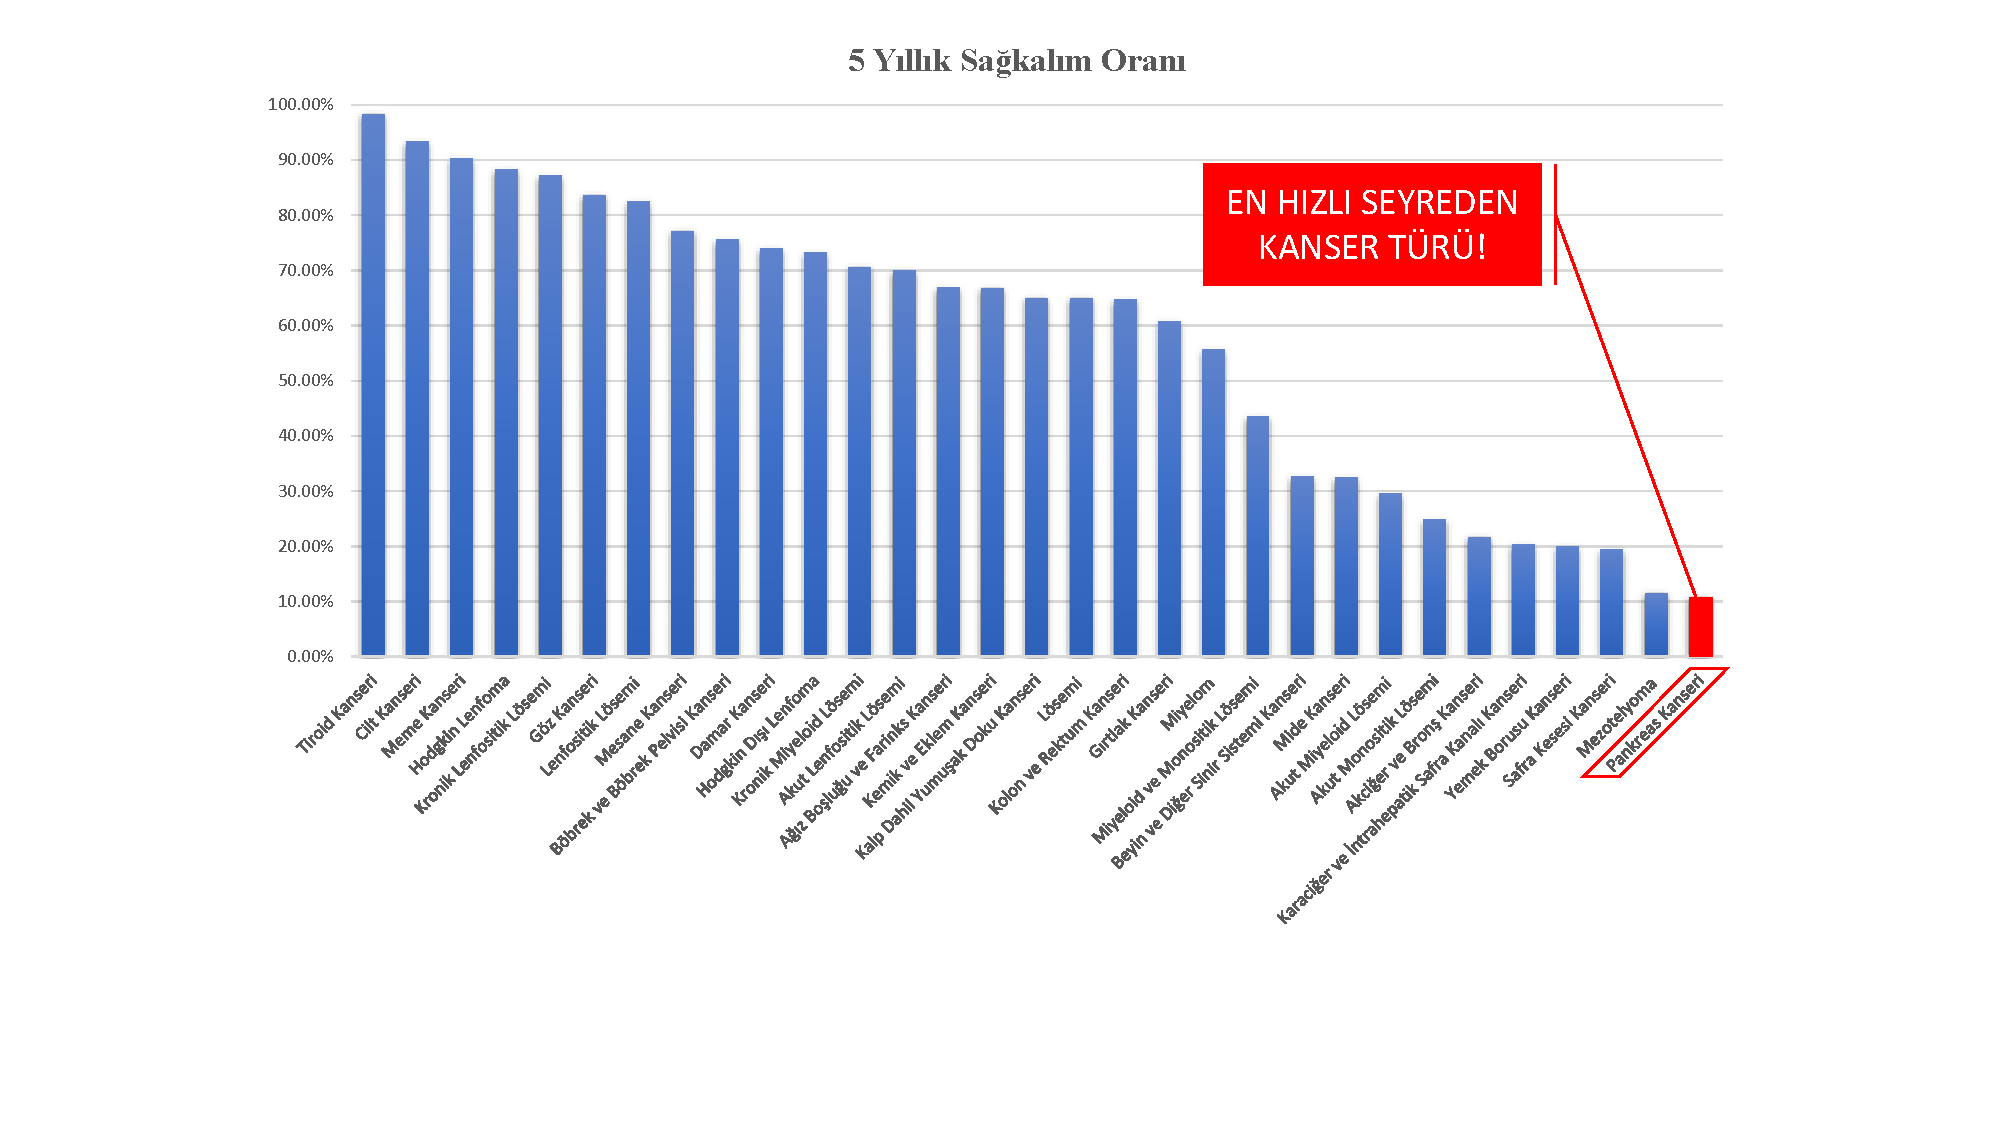
\includegraphics[scale=0.62]{Genel-Bilgiler/Figures/seer_statistic.pdf}
		}
	\end{center}
\end{figure}

Pankreas kanseri sürecinde hastalığa yakalanma ve hastalığa bağlı ölüm arasında geçen süreye bakıldığında, bu sürenin oldukça kısa sürdüğü gözlemlenmektedir. The Surveillance, Epidemiology, and End Results (SEER) Programı Amerika'daki bazı eyaletlerdeki kanser istatistiklerini raporlayan bir kuruluştur \cite{pancreasistatisticseer}. 1973 yılından beri istatistiksel bilgiler bu kuruluş tarafından toplanmakta ve kanser hastalarının istatistiksel verilerinin yorumlanmasına dair en geniş katılımlı ve en güvenilir verileri sağlamaktadır. Şekil \ref{fig:seer_stat}'de verilen SEER 18, (2011-2017) yılları arasında karşılaşılan kanser hastalarının 5 yıllık sağkalım oranlarına bakıldığında en hızlı seyreden kanser türünün pankreas kanseri olduğu görülmektedir. 

Pankreas kanserli hastalarda 5 yıllık sağkalım oranı Amerika Birleşik Devletleri'nde \%10’a kadar düşmektedir. Bu oran diğer kanser türlerine göre oldukça düşüktür. Bu düşük sağkalım oranının en önemli sebebi hastalığın teşhisinin geç konmasıdır. Pankreas kanseri ile mücadele eden hastaların çoğu, hastalık ileri bir aşamaya gelinceye kadar asemptomatiktir.

Pankreas kanseri 5 yıllık sağ kalım oranının bu kadar yüksek olmasının başlıca sebebi erken teşhisinin oldukça zor olmasıdır. Bu sebeple pankreasın konumsal ve şekilsel zorluğu düşünüldüğünde doktorlara yardımcı bir bilgisayar destekli teşhis sisteminin önemi ortaya çıkmaktadır. Pankreas kanserinde ön teşhis genellikle Bilgisayarlı Tomografi (BT), Magnetik Rezonans (MR) gibi volümetrik veri üreten ve doktor tarafından işlenerek çıkarımda bulunulması zahmetli görüntüleme teknikleri ile gerçekleştirilmektedir. Bilgisayar destekli sistemler bu tür verilerin işlenerek doktorların daha kolay çıkarımda bulunabilmelerine imkan tanıyabilmektedir.

\section{Pankreas Organı Konumu ve Görevi}
Pankreas organı salgıladığı enzimler ile sindirim sistemi ve kan şekeri seviyelerinin kritik kontrolünde önemli rol oynayan iki işlevli uzun yassı hormonal bir bezdir \cite{bockman1993anatomy}. Hem iç hem de dış salgı bezi olarak görev yapmaktadır. Bu yüzden karma bez olarak da adlandırılmaktadır. Pankreas organı ortalama olarak 15-25 cm uzunluğuna sahip olup erkeklerde ortalama 75 gr kadınlarda ise ortalama 55 gr ağırlığına sahiptir. Pankreasın düzensiz biçimi önden arkaya doğru yassılaşmakta ve bir çengele benzetilebilmektedir. Pankreas organının anatomik yapısı Şekil \ref{fig:pank_anat}'de verilmektedir. Şekilde görüldüğü gibi pankreas anatomik yapı olarak pankreas adacıkları, safra kanalı, pankreas hormonları ve asiner hücrelerinden oluşmaktadır. İnsülin, glukagon ve somatostanin pankreas hormonlarındandır. Pankreas adacıkları ise alfa, beta ve delta hücrelerinden oluşmaktadır. Yapısal olarak baş, boyun, gövde ve kuyruk olmak üzere temelde 4 ayrı bölgeye ayrılabilmektedir. 

\captionsetup[figure]{margin={0.3cm,0cm}}
\begin{figure}[h!]
	\begin{center}
		\vspace{0.4cm}
		\captionbox{Pankreas organının anatomik yapısı\cite{pancreasimage}
		\label{fig:pank_anat}}
		{
			\vspace{0.4cm}
			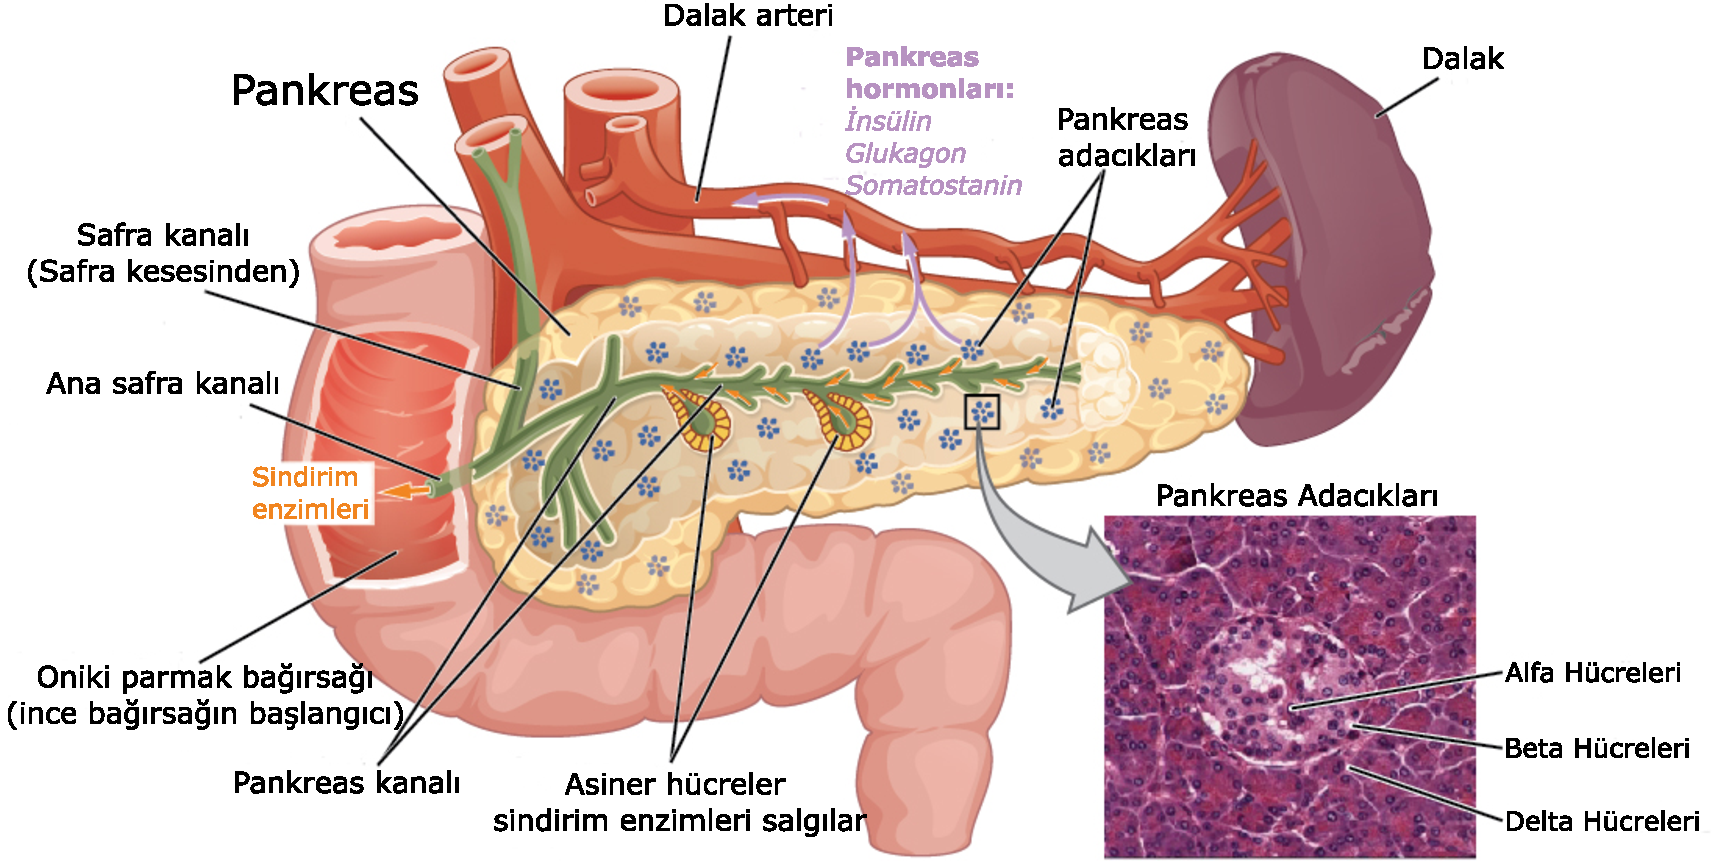
\includegraphics[scale=0.52]{Genel-Bilgiler/Figures/pankreas.pdf}
		}
	\end{center}
\end{figure}

Pankreas organı konumsal olarak bazı önemli ana taşıyıcı damarlara da oldukça yakın pozisyonda bulunmaktadır. Vücudumuzdaki en büyük atardamar olan Aort damarı ve alt ana toplar damar pankreasın baş bölgesinin hemen arkasında kalmaktadır. Ana atar ve toplar damarların geçtiği kodumda yer almasından dolayı yine birçok önemli damar ile birebir ilişki içerisindedir. Bu sebeple pankreas organında ortaya çıkan kitleler aşırı büyüdüğünde önemli damarların daralmasına ve buna bağlı olarak sarılık, damar tıkanıklığı gibi oldukça ölümcül hastalıklara sebebiyet verebilmektedir.

Şekil \ref{fig:pank_konum}’ de görüldüğü gibi pankreas organı konum olarak abdominal (karın, göbek) bölgede yer almaktadır.  Pankreas organı karnın arka bölümünün ortasında olup, sağ kısmı mide ile omurga arasında yer alırken, kuyruk kısmı soldan on iki parmak bağırsağının kıvrımına (ince bağırsağın ilk kısmı) kadar uzanmaktadır \cite{bockman1993anatomy,skandalakis1993surgical}.

\captionsetup[figure]{margin={0.9cm,0cm}}
\begin{figure}[h!]
	\begin{center}
		\vspace{0.4cm}
		\captionbox{Pankreas organının vücuttaki konumu \cite{pancreaslocationimage}
		\label{fig:pank_konum}}
		{
		    \vspace{0.1cm}
			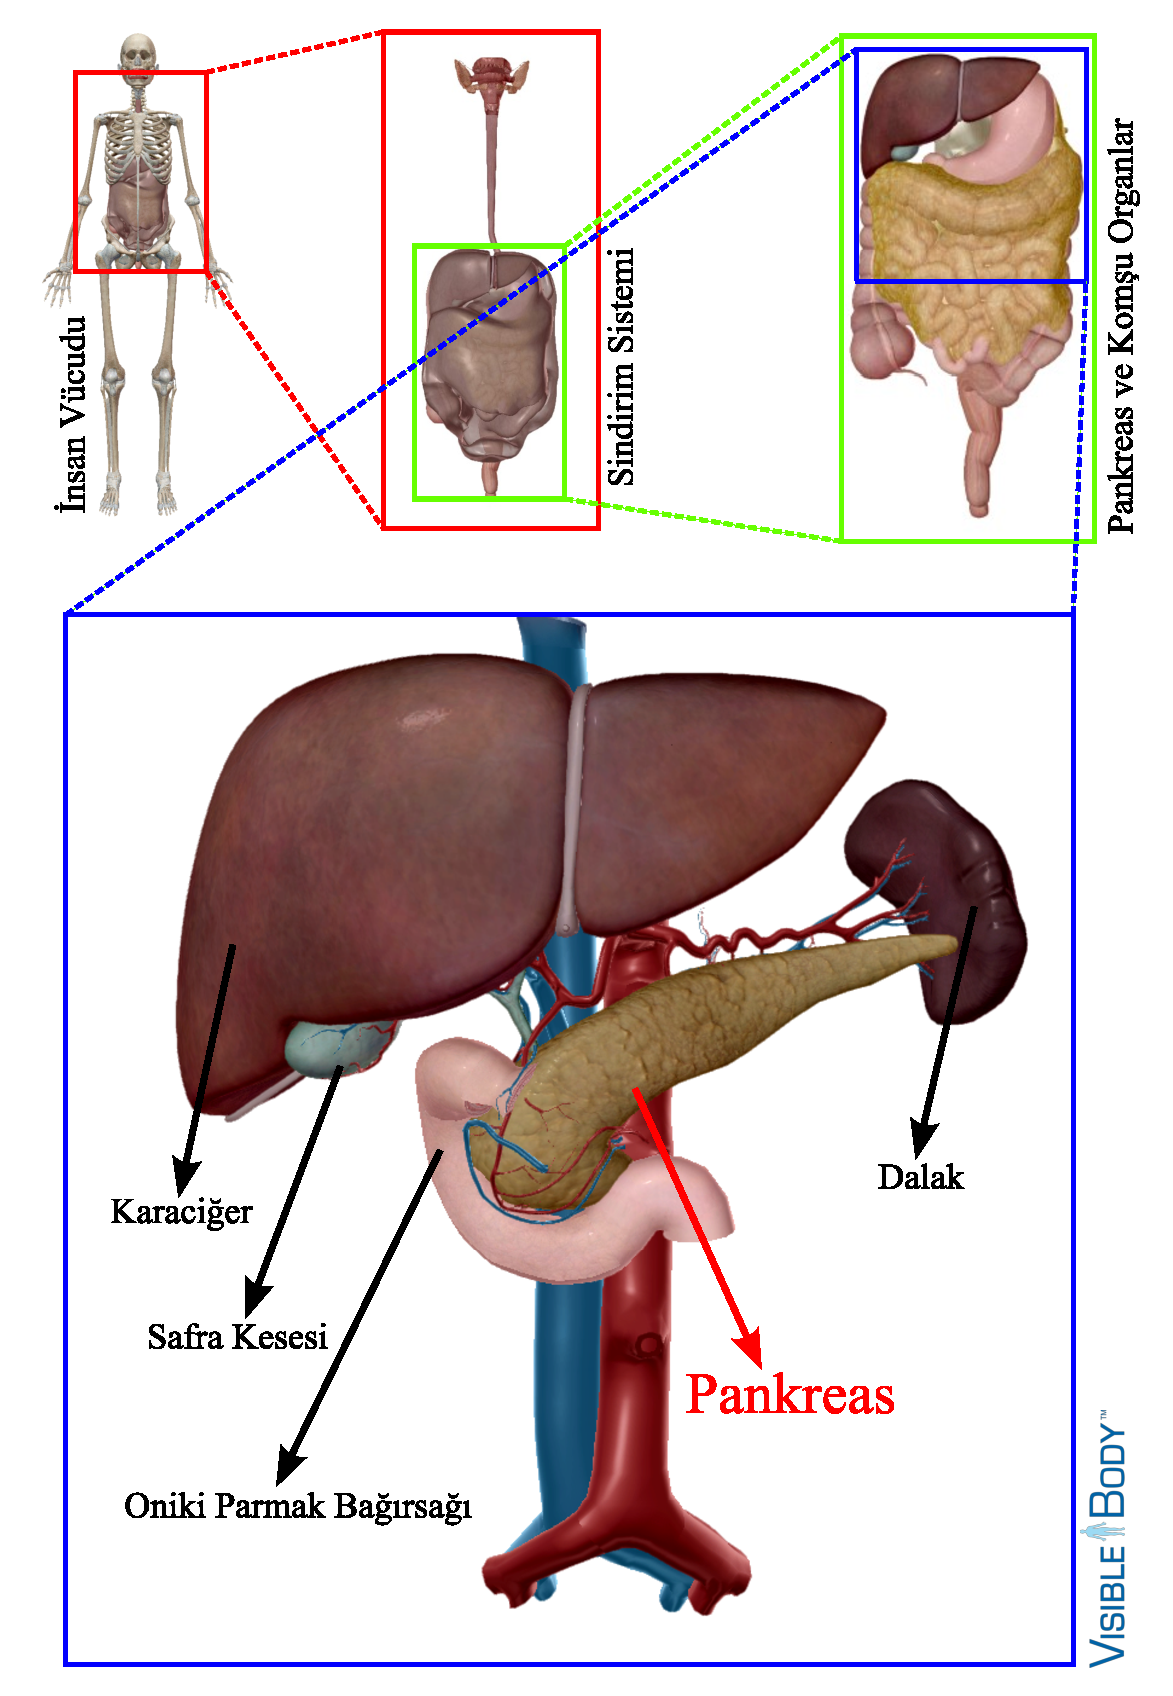
\includegraphics[scale=0.66]{Genel-Bilgiler/Figures/pankreas_location.pdf}
		}
	\end{center}
\end{figure}

Pankreas organının vücudumuzda oldukça önemli iki ana işlevi bulunmaktadır. Bunlar sindirime yardımcı olan sindirim enzimlerinin üretilmesinde rol alan ekzokrin işlevi ve kan şekerini düzenleyen insülin, glukagon gibi hormonların salgılanmasını sağlayan endokrin işlevidir [3-5]. Ekzokrin ve endokrin işlevleri şu şekilde açıklanabilmektedir:

-  Ekzokrin İşlevi:

Şekil \ref{fig:pank_ekzokrin}’te görüldüğü gibi pankreas organı, sindirim için önemli enzimler üreten ekzokrin bezleri içermektedir. Bu enzimlerin görevi ve isimleri sırasıyla şu şekildedir: protein sindirmek için tripsin ve kimotripsin; karbonhidratların sindirimi için amilaz; ve yağları parçalamak için lipaz. Yiyecek mideye ulaştığı zaman, pankreas özsuları ana pankreas kanalına ulaşan kanal sistemine salınmaktadır. Pankreas kanalı, duodenum adı verilen ince bağırsağın ilk kısmında yer alan Vater ampullasını oluşturmak için ortak safra kanalına katılmaktadır. Ortak safra kanalı, karaciğer ve safra kesesinden oluşmakta olup safra adı verilen bir başka önemli sindirim suyu üretmektedir. Oniki parmak bağırsağına salınan pankreas özsuları ve safra, vücudun yağları, karbonhidratları ve proteinleri sindirmesine yardımcı olmaktadır.

\captionsetup[figure]{margin={0.3cm,0cm}}
\begin{figure}[h!]
	\begin{center}
		\vspace{0.4cm}
		\captionbox{Pankreas organının Ekzokrin işlevi \cite{pancreaslocationimage}.
			\label{fig:pank_ekzokrin}}
		{
			\vspace{0.4cm}
			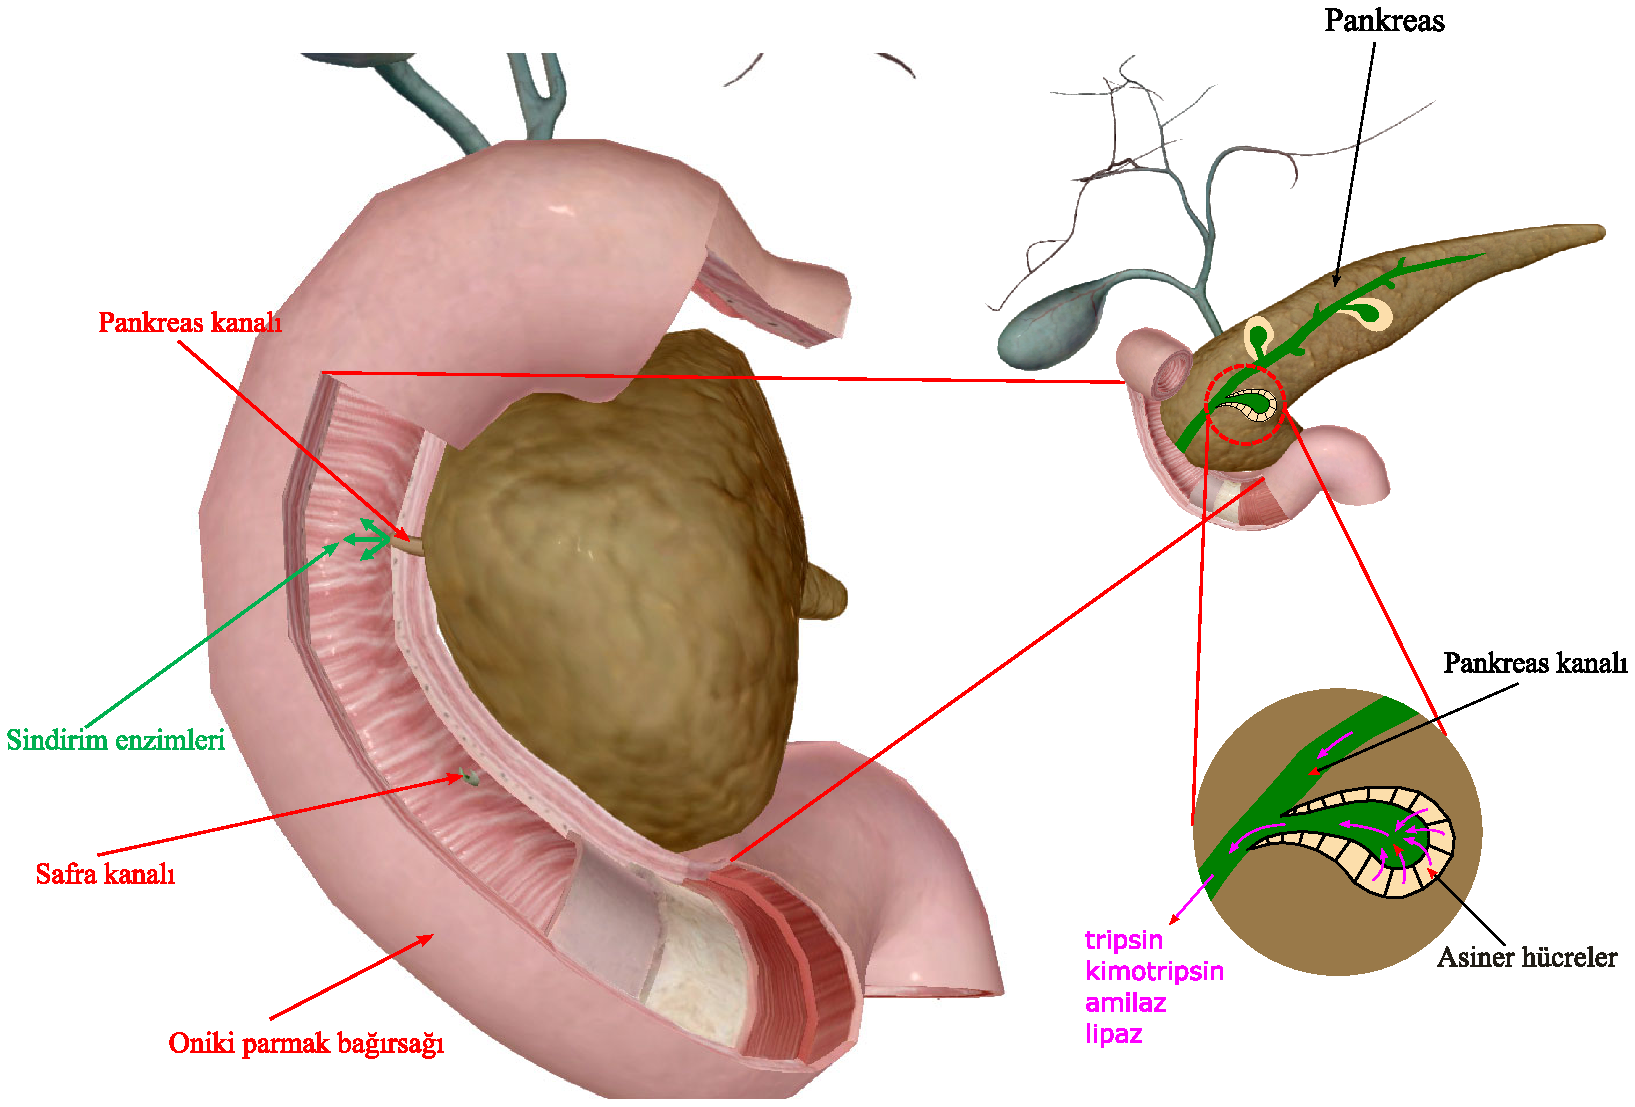
\includegraphics[scale=0.55]{Genel-Bilgiler/Figures/ekzokrin_function.pdf}
		}
	\end{center}
\end{figure}

- Endokrin İşlevi:

Pankreasın endokrin bileşeni, Şekil \ref{fig:pank_endokrin}’te görüldüğü gibi önemli hormonları oluşturan ve doğrudan kan dolaşımına salan adacık hücrelerinden oluşmaktadır. Adacık hücrelerinin yaklaşık \%70'i beta hücrelerinden, \%20'si alfa hücrelerinden ve \%10'u delta hücrelerinden oluşmaktadır. Bu hücrelerden beta hücreleri insülin, amilin hormonlarını, alfa hücreleri glukagon hormonunu, Delta hücreleri ise somatostatin hormonunu üreterek damarlar vasıtası ile kana iletilmektedir \cite{krahl1974endocrine}. Bu hormonların en önemli görevi kan şekerini dengelemektir.  Uygun kan şekeri seviyelerini korumak, beyin, karaciğer ve böbrekler dahil olmak üzere kilit organların işleyişi için çok önemlidir.


\captionsetup[figure]{margin={0.4cm,0cm}}
\begin{figure}[h!]
	\begin{center}
		\vspace{0.4cm}
		\captionbox{Pankreas organının Endokrin işlevi \cite{pancreaslocationimage}.
			\label{fig:pank_endokrin}}
		{
			\vspace{0.4cm}
			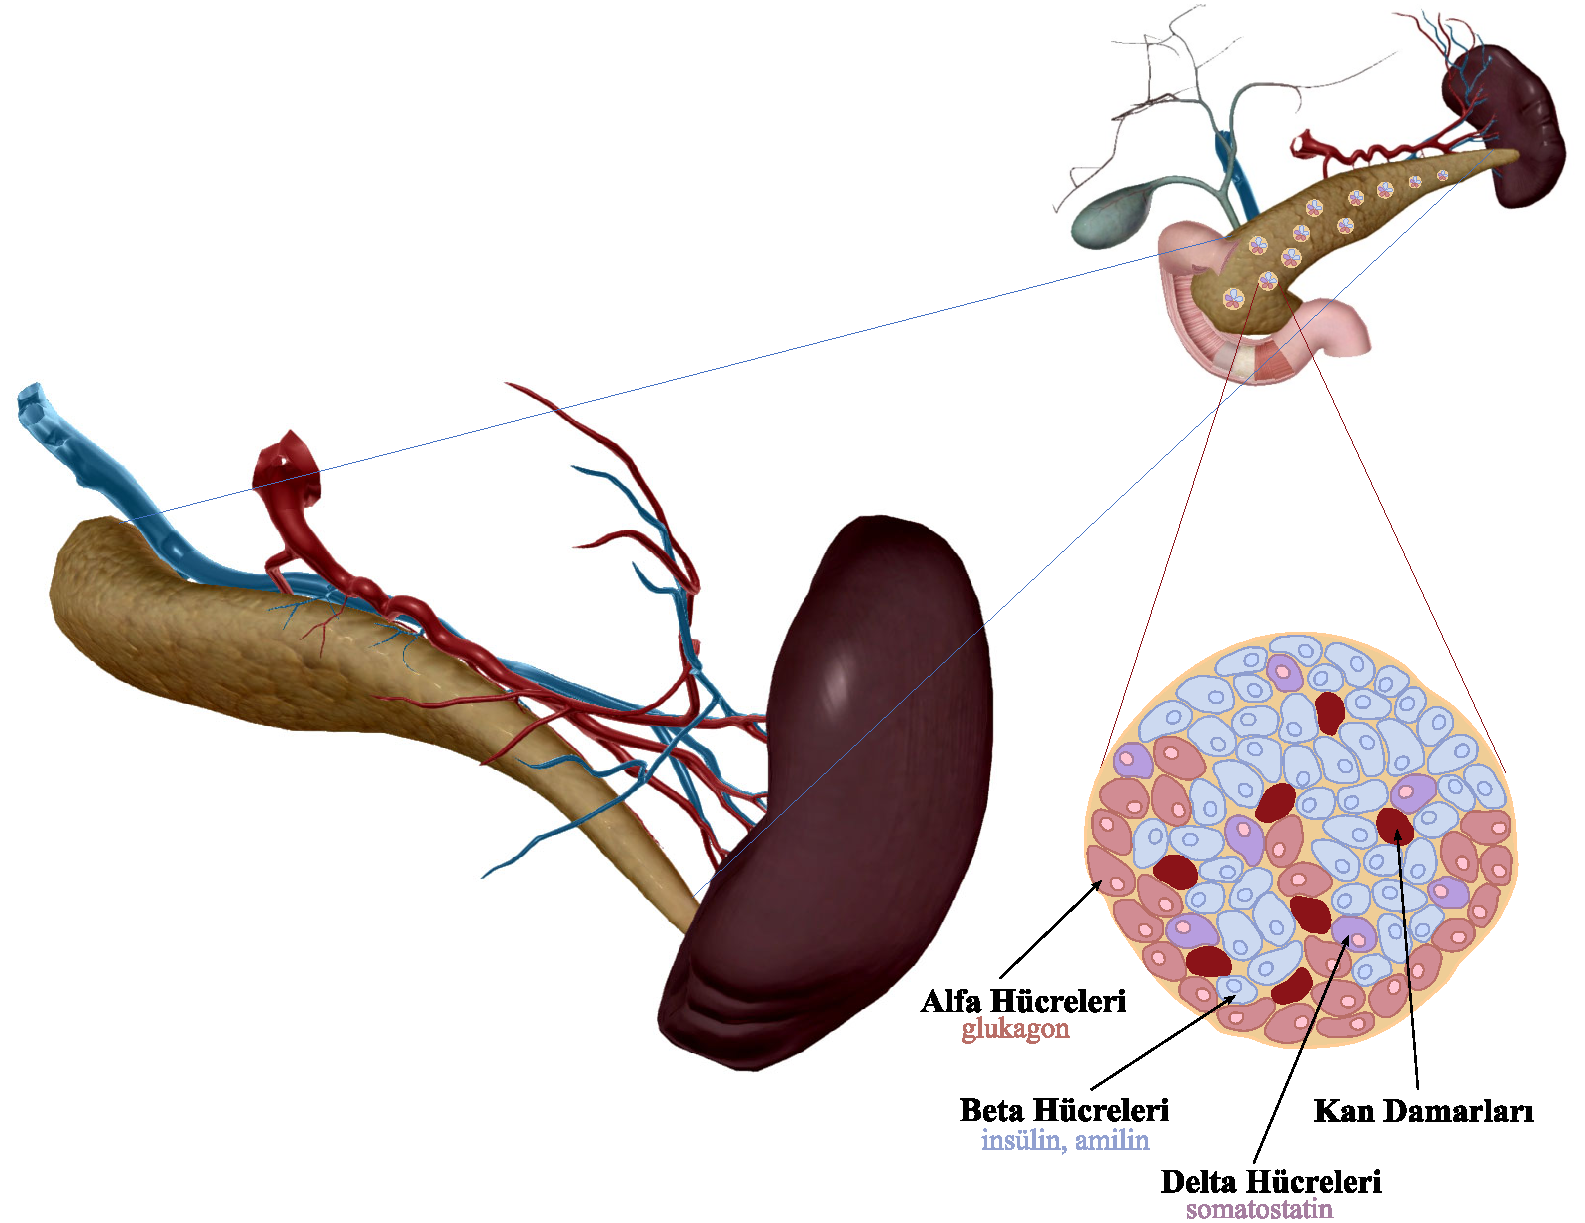
\includegraphics[scale=0.57]{Genel-Bilgiler/Figures/endokrin_function.pdf}
		}
	\end{center}
\end{figure}

\section{Pankreas ve Pankreas Kanseri Görüntüleme Teknikleri}

Günümüzde pankreas kanseri tanısı, tümörlü dokuların konumunun tespiti ve hastalığın evrelendirilebilmesi gibi amaçlar için Ultrason, Endoskopik Ultrason (EUS), Bilgisayarlı Tomografi (BT), Manyetik Rezonans (MR), Endoskopik Retrograd Kolanjiopankreatografi (ERCP), İnce İğne Aspirasyonu gibi teknikler ön plana çıkmaktadır \cite{goral2014pankreas,freelove2006pancreatic,cameron2001pancreatic,chu2017diagnosis}.

Görüntüleme tekniğinin hasta bireylerin tanılanmasında gösterdiği başarı Duyarlılık olarak adlandırılmaktadır. Yine ilgili görüntüleme tekniğinin sağlıklı bireylere tanı koymada gösterdiği başarıya da Özgüllük denilmektedir. Görüntüleme tekniklerinin bir hastalığa tanı konmasında kullanılabilmesi için ilgili testin Özgüllük (\%) ve Duyarlılık (\%) değerlerinin toplamının 170 değerinden büyük olması beklenmektedir. Ayrıca pankreas kanseri gibi kanser dokularının oluşturduğu tümörlü bölgenin ebatları ve konumu hastalığın evrelenmesinde önemli rol oynamaktadır. Bu sebeple pankreas kanserine tanı konmasında kullanılacak görüntüleme tekniğinin Duyarlılık ve Özgüllük metriklerinin dışında hastalığın evrelendirilmesindeki başarısı da önem arz etmektedir.

\begin{table}[h!]	
	\caption{Pankreas kanseri tanı ve evrelendirmesinde kullanılan başlıca görüntüleme yöntemleri.\cite{goral2014pankreas}}
	\begin{tabular}{m{6cm}m{2.5cm}m{2.5cm}m{3cm}}
		& \textbf{Özgüllük} & \textbf{Duyarlılık} & \textbf{Evrelemede Fayda} \\ \hline
		Ultrason                                              & 80\%     & 90\%       & YOK                   \\ \hline
		Endoskopik Ultrason (EUS)                             & 90\%     & 90\%       & VAR                   \\ \hline
		Endoskopik Retrograd Kolanjiopankreotografi (ERCP) & 90\%     & 90\%       & YOK                   \\ \hline		
		İnce İğne Aspirasyonu                                 & 90\%     & 98\%       & YOK 
		\\ \hline
		Magnetik Rezonans (MR)                                & 90\%     & 90\%       & YOK                   \\ \hline
		\rowcolor{Gray}
		Bilgisayarlı Tomografi (BT)                           & 90\%     & 95\%       & VAR                                    
	\end{tabular}
	\label{tab:goruntulemeteknikleri}
\end{table} 

Tablo \ref{tab:goruntulemeteknikleri}'de görüldüğü gibi BT görüntüleme pankreas kanserini evreleme aşamasında en fayda sağlayan görüntüleme tekniğidir. Bu teknik en yüksek Özgüllük ve Duyarlılık seviyelerine sahip olan görüntüleme tekniği olarak ön plana çıkmaktadır. Dolayısıyla pankreas kanserine tanı konması ve evrelendirilmesi için çoğunlukla BT görüntüleme tekniği tercih edilmektedir.

\subsection{Ultrason}

Ultrason pankreas kanseri belirtilerinden olan karın ağrısı ve sarılık gibi durumlarla karşılaşıldığında daha uygun maliyetli olması ve insan sağlığına daha az zararlı olması gibi sebeplerden dolayı öncelikle tercih edilen görüntüleme tekniği olarak karşımıza çıkmaktadır \cite{wells2006ultrasound,chan2011basics,sofuni2005differential}. Ultrasonun çalışma prensibi yüksek frekanslı ses dalgalarının farklı dokulardan farklı miktarlarda yansıma yapmasına dayalıdır. Ultrason cihazını kullanan operatörün yetenekleri ve bağırsak gazlarının pankreas dokusunu maskelemesi gibi durumlar bu görüntüleme tekniğinin Özgüllük ve Duyarlılığını fazlasıyla etkilemektedir. Bu sebeple genellikle ilk teşhisin koyulmasında kullanılmakta sonrasında ise daha gelişmiş görüntüleme tekniklerine ihtiyaç duyulmaktadır.

\subsection{Endoskopik Ultrason (EUS)}

Bu görüntüleme tekniği, endoskopik yoldan sindirim sistemini oluşturan yemek borusu, mide, pankreas, karaciğer, safra kesesi ve bağırsaklar gibi organlarda ortaya çıkabilen kitle ve lezyonların tanı, teşhis ve evrelendirilmesinde sıklıkla kullanılmaktadır. Endoskopik yoldan salınan esnek kablo ucundan yüksek frekanslı ses dalgaları gönderilerek endoskopik yol etrafındaki farklı yoğunluklu organlardan yansıyan ses dalgaları kullanılması prensibine dayalı bir görüntüleme tekniğidir. Ultrasona göre çok daha hassas bir görüntüleme sağlayabilmektedir. Pankreas kanserinin ve tümörlü dokuların ilk teşhisinde sıklıkla tercih edilmektedir\cite{rosch1991endoscopic,anderson2000endoscopic}. Ultrasonda olduğu gibi cihazı kullanan operatörün yetenekleri ve ilgili bölgedeki bağırsak gazı yoğunluğu bu görüntüleme tekniğinin Özgüllük ve Duyarlılığını fazlasıyla etkilemektedir.

\subsection{Endoskopik Retrograd Kolanjiopankreatografi (ERCP)}	

Bu görüntüleme tekniğinde endoskopik yoldan ucunda ışıklı kamera bulunan özel bir endoskopi cihazı ile yemek borusu üzerinden mideye ve mideden de oniki parmak bağırsağına ulaşılmaktadır. Oniki parmak bağırsağına bağlanan milimetrik boyutlardaki safra kanalı üzerinden de ince uçlu kateter denilen cihazlarla safra kanalına yada pankreas kanalına kontrast madde enjekte edilmektedir. Daha sonra x ışınları kullanan bir cihaz ile enjekte edilen kontrast maddenin ilgili dokularda görüntülenmesi sağlanarak taş ve tümör gibi anormalliklerin teşhisi sağlanmaktadır \cite{oi1998ercp,hanada2019roles}. Kontrast maddenin direk hedef bölgeye uygulanmasından dolayı daha kullanışlı sonuçlar elde edilebilmektedir. Bu işlem genel olarak güvenli olmakla beraber bazı istenmeyen yan etkilerle karşılaşılabilmektedir \cite{mallery2003complications}. Özellikle pankreas tümörlerinin tespitinde kullanıldığında pankreas bezlerinin iltihaplanması (pankreatik) durumu ile karşılaşılabilmekte ve tümör evrelemede yeterli görülmemektedir.

\subsection{İnce İğne Aspirasyonu}

Bu teknikte ince uçlu bir iğne ile kanser şüphesi bulunan kitlelere genellikle endoskopik ultrason rehberliği ile ulaşılarak doku örneği alınmaktadır \cite{robins1995fine,harewood2002endosonography,frossard2003performance}. Öncelikle vücudun dışından iğne ile giriş yapılacak bölge lokal olarak uyuşturulmaktadır. Daha sonra lokal uyuşturulan bu bölgeden girilerek hedef kitleye ulaşılmaktadır. Bu teknikle elde edilen doku örnekleri incelenelerek kitlenin türüne göre tanı ve tedavi prosedürleri uygulanabilmektedir. Genellikle işlem bir sitopatalog eşliğinde yapılmaktadır. Sitapatoloğun mesleki deneyimi alınan doku örneklerine tanı konmasında yeterli olması oldukça önemlidir. Bu yöntemde kitle bütünlüğü ve pankreasa komşu organlarla ilişkisi görüntülenemediği için hastalığı evrelemede fayda sağlamamaktadır. 

\subsection{Manyetik Rezonans (MR)}

İnsan vücudundaki organ ve dokuların, radyo dalgaları ve manyetik alanların kullanılmasıyla detaylı ve yüksek çözünürlüklü görüntülenebilmesi için kullanılan bir görüntüleme tekniğidir \cite{reimer2010clinical,semelka1993mr,tirkes2012mr}. Bilgisayarlı Tomografi görüntüleme tekniğinin aksine x-ray ışınları ve iyonize radyasyon içermediği için insan sağlığına çok daha az zararlıdır. MR genellikle beyin omurilik hastalıkları, kas yaralanmaları ve nörolojik hastalıkların teşhisinde tercih edilmektedir. Bazı özel durumlarda pankreas tümörü tespitinde başarılı sonuçlar verebilmektedir. Fakat genellikle pankreas kanseri evreleme aşamasında yeterli görülmemektedir. Kalbinde pil yada stent takılı, dişlerinde tel takılı yada vücudunda herhangi çelik içerikli protez bulunan hastalarda manyetik çekim gücünün sebep verebileceği hasarlardan dolayı kullanılamamaktadır.

\subsection{Bilgisayarlı Tomografi (BT)} 

Bilgisayarlı tomografi (BT) insan vücudunun, organlarının, iskelet sisteminin ve diğer dokuların detaylı volumetrik görüntülerinin oluşturulması için x-ışınlarının kullanıldığı radyolojik bir görüntüleme tekniğidir. Bilgisayarlı tomografi cihazları temelde hastanın üzerinde uzandığı yatay eksende hareketli tabya, tabya etrafında dairesel dönen x-ışını üretici ve yine tabya etrafında dönen ve x-ışını üreticinin karşısına konumlandırılmış x-ışını dedektöründen oluşmaktadır \cite{kalender2011computed,seeram2015computed}. X-ışını üreticisinden üretilen ışınlar hasta vücudundaki farklı yoğunluklu dokulardan geçerken farklı miktarda zayıflamaya maruz kalarak x-ışını dedektörü tarafından yakalanmaktadırlar. Şekil \ref{fig:ct_block}'da bilgisayarlı tomografi (BT) cihazının çalışma prensibi görselleştirilmektedir. Burada da görüldüğü gibi x-ışını dedektörü tarafından algılanan farklı miktarlarda zayıflamaya uğramış x-ışınları işlenerek yatay vücut kesit görüntüleri elde edilmektedir. 

\captionsetup[figure]{margin={0.4cm,0cm}}
\begin{figure}[h!]
	\begin{center}
		\vspace{0.4cm}
		\captionbox{Bilgisayarlı tomografi (BT) cihazının çalışma prensibi.
			\label{fig:ct_block}}
		{
			\vspace{0.4cm}
			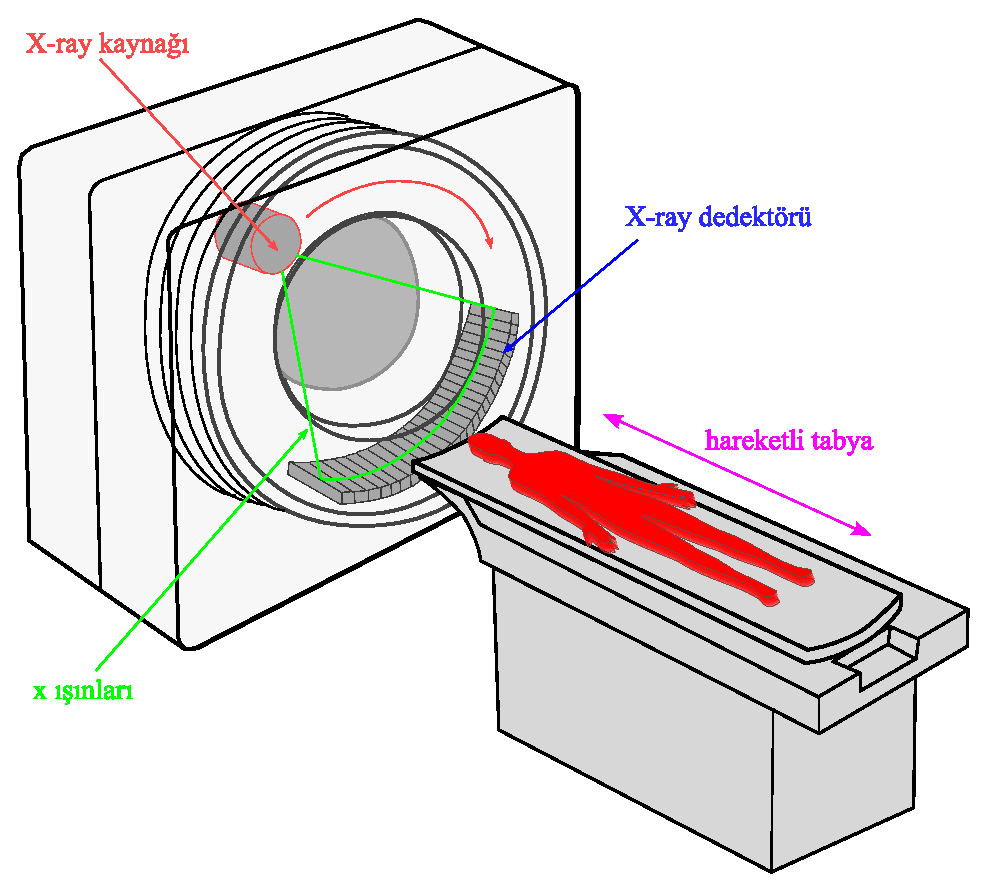
\includegraphics[scale=0.68]{Genel-Bilgiler/Figures/ct_block.pdf}
		}
	\end{center}
\end{figure}

Sıralı elde edilen bu kesit görüntüleri birleştirilerek volumetrik vücut verisi üretilmektedir. Bu volumetrik verideki her 3B piksel voksel olarak adlandırılmaktadır. Piksel ifadesi matris boyutu ve görüş alanına bağlı iki boyutlu bir birimken, BT diliminin kalınlığı da dikkate alındığında bilgisayarlı tomografi görüntüleme tekniğindeki üç boyutlu bir birim olan voksel terimi tercih edilmektedir. Volumetrik BT taramasındaki her bir dilimin üretilmesinde Şekil \ref{fig:ct_hounsfield}'de gösterilen ve Hounsfield ölçeği denilen bir ölçeklendirme tekniği kullanılmaktadır. Hounsfield ölçeğinde x-ışınlarında en çok zayıflamaya sebep veren dokuların voksel değeri +3071 ile temsil edilirken en az zayıflamaya sebep olan dokuların voksel değeri ise -1024 ile temsil edilmektedir \cite{hounsfield1973computerized}.

\captionsetup[figure]{margin={0.5cm,0cm}}
\begin{figure}[h!]
	\begin{center}
		\vspace{0.4cm}
		\captionbox{Bilgisayarlı tomografi (BT) Hounsfield ölçeği ile volumetrik veri elde edilmesi.
			\label{fig:ct_hounsfield}}
		{
			\vspace{0.4cm}
			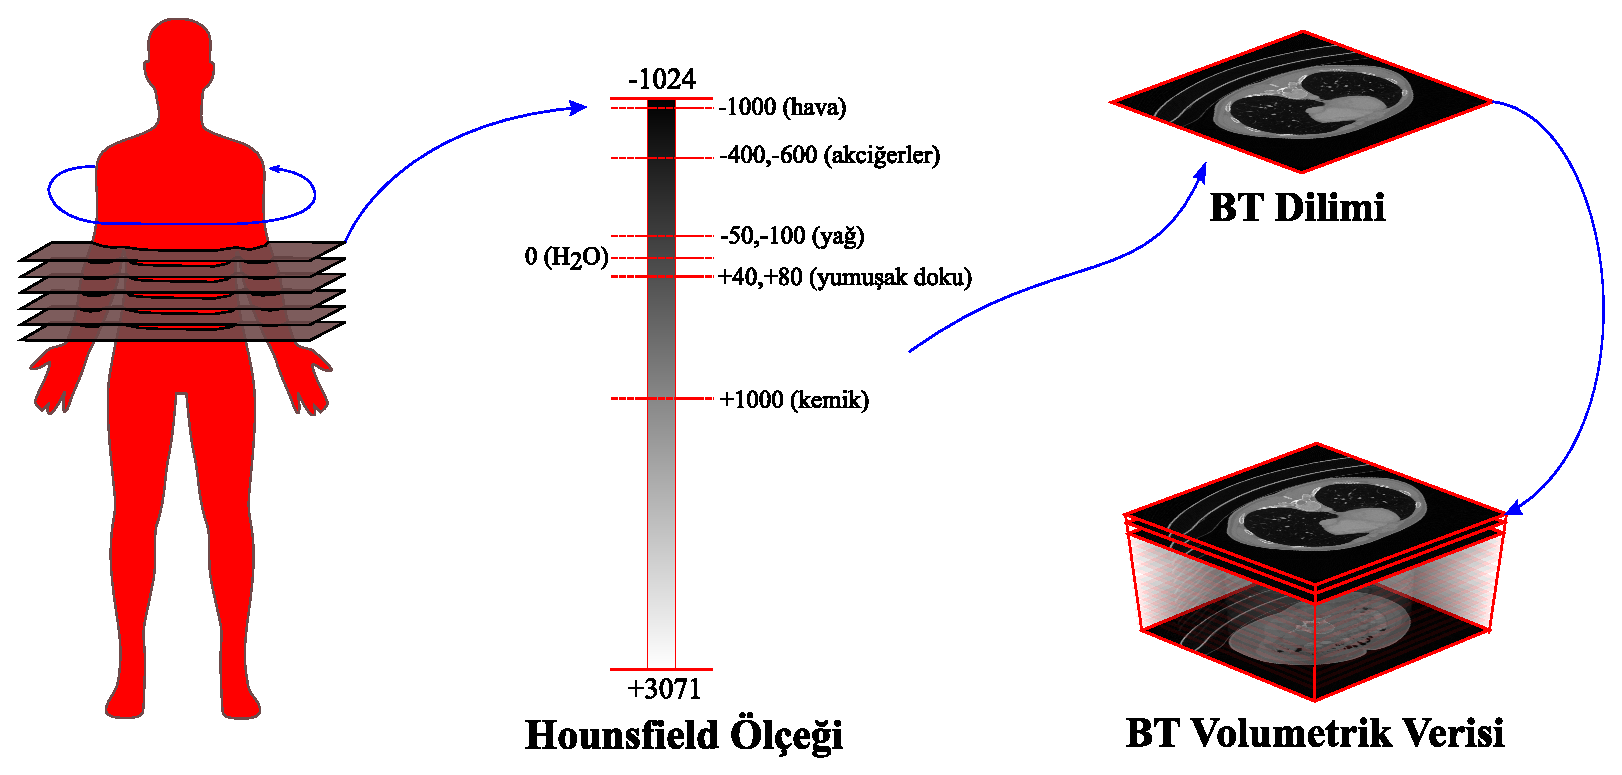
\includegraphics[scale=0.55]{Genel-Bilgiler/Figures/ct_hounsfield.pdf}
		}
	\end{center}
\end{figure}

Bilgisayarlı tomografi görüntüleme tekniği yaralanma, kalp hastalıkları, kemik, eklem ve doku zedelenmesi, organlar ve organlarda ortaya çıkan kitleler gibi anomalilerin tespiti, zatürre gibi akciğer hastalıklarının tespiti gibi çok çeşitli alanlarda doktorlara müdahale öncesinde önemli ön bilgiler sunabilmektedir. Özellikle pankreas hastalıkları ve pankreas kitlelerinin detaylı incelemelerinde sıklıkla tercih edilmektedir. Tablo \ref{tab:goruntulemeteknikleri}'de görüldüğü gibi diğer görüntüleme tekniklerine göre daha üstün tanılama bilgileri sağlamaktadır. Bu sebeple pankreas organının zor konumu ve fizyolojik yapısı düşünüldüğünde bilgisayarlı tomografi oldukça kritik bir görüntüleme tekniği olarak karşımıza çıkmaktadır. 

İnsan vücudu anatomik olarak incelendiğinde pankreas organı head, thorax, abdomen ve pelvis gibi bölgelerden abdomen bölgesinde yer almaktadır. Bu sebeple pankreas hastalıkları için bilgisayarlı tomografi görüntüleme tekniği kullanıldığında abdomen bölgesi için tarama gerçekleştirilmektedir. Pankreastaki kitlelerin bilgisayar destekli tanılama sistemlerince işlenebilmesi amacıyla abdomen bölgeden volumetrik görüntüler alınmaktadır. Volumetrik bilgisayarlı tomografi görüntülerinin her biri uzman kişilerce pankreas ve tümör dokularının bulunduğu bölgelerin işaretlenmesi için incelenmektedir. Bu sayede Şekil \ref{fig:pancreas_abdomen}'deki gibi veri setleri üretilebilmektedir. 

\captionsetup[figure]{margin={0.3cm,-1cm}}
\begin{figure}[h!]
	\begin{center}
		\vspace{0.4cm}
		\captionbox{Abdomen bölgeden elde edilen volumetrik BT verisinin manuel olarak işaretlenmesi ile oluşturulan pankreas bölgesi \cite{pancreaslocationimage}.
			\label{fig:pancreas_abdomen}}
		{
			\vspace{0.4cm}
			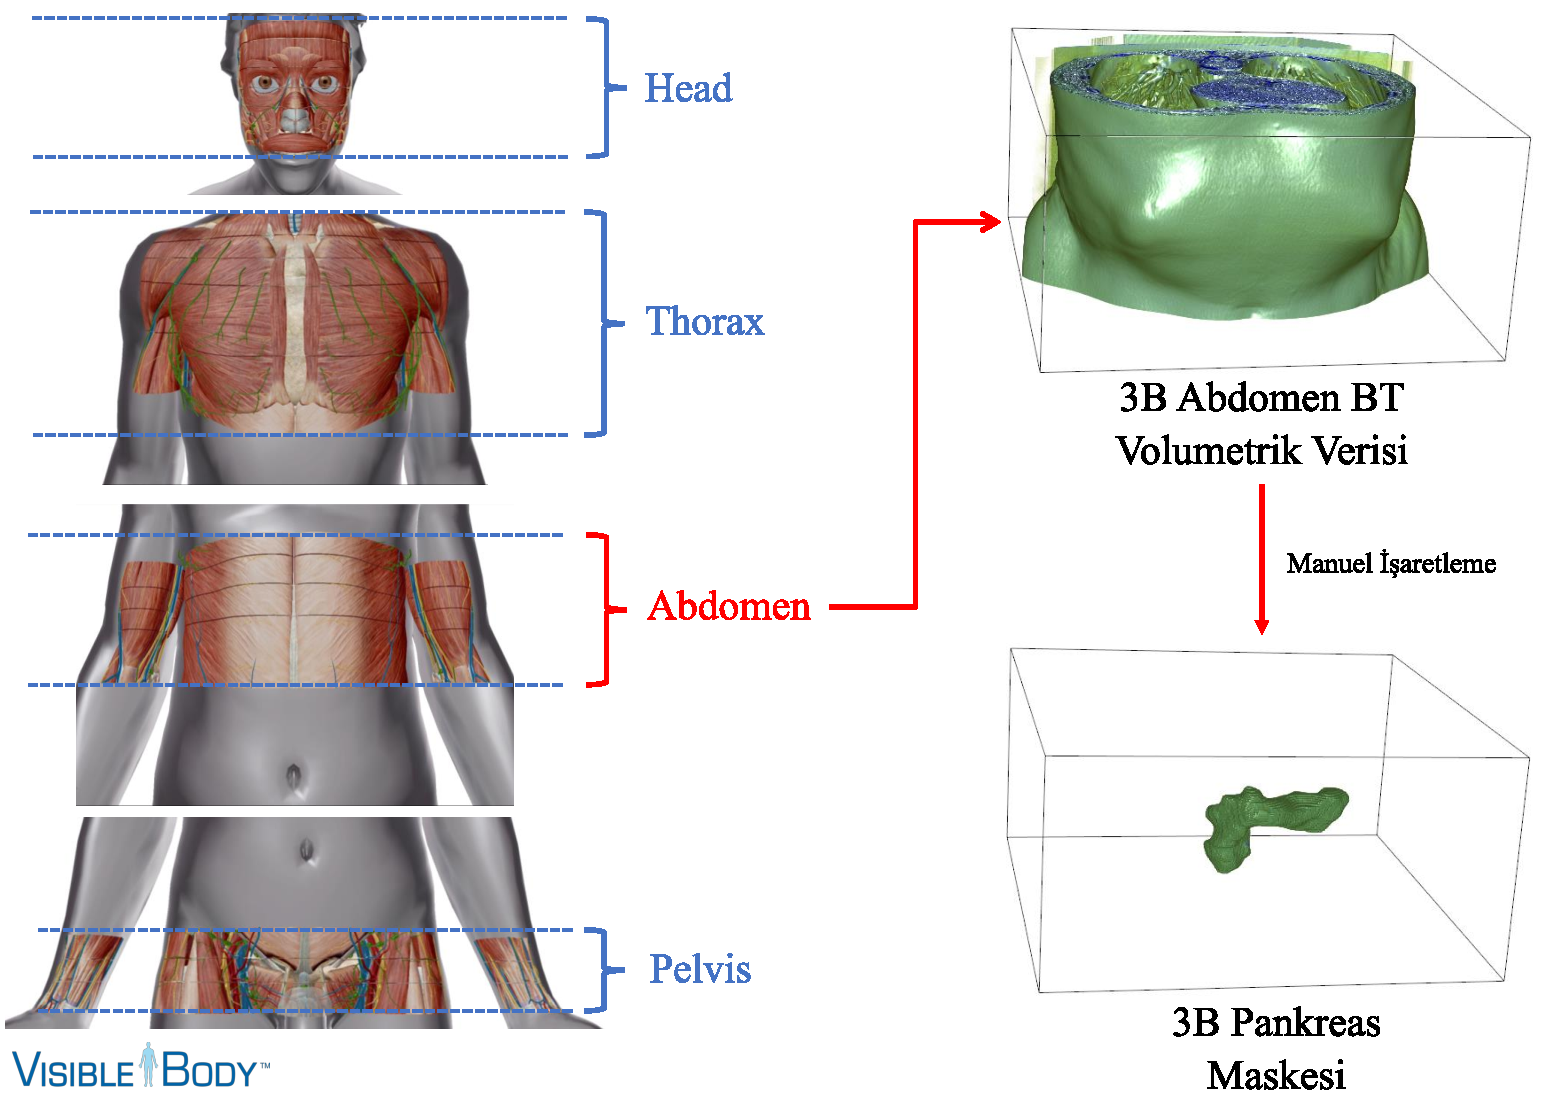
\includegraphics[scale=0.5]{Genel-Bilgiler/Figures/pancreas_abdomen.pdf}
		}
	\end{center}
\end{figure}

\section{Tez Çalışmasında Kullanılan Veri Setleri}
Tez çalışmamızda literatürdeki çalışmalara göre BT görüntülemede daha yüksek doğrululuğa sahip otomatik pankreas ve pankreas tümörü segmentasyonu sağlamak amaçlanmaktadır. Bu kapsamda pankreas ve pankreas tümör segmentasyonu için CNN tabanlı yaklaşımlar geliştirilmektedir. 

Tez çalışmasının ilk kısmında pankreas segmentasyonu için ilgi bölgesi belirlenerek bölge küçültme tekniği ile çalışan bir yöntem önerilmektedir. Önerilen yöntemde veri setinin iki sınıflı (pankreas, diğer dokular) olması, kanser dokularının segmentasyonunu içermemesi ve daha basit işlenebilir olmasından dolayı Ulusal Sağlık Enstitüleri Pankreas BT Veri Seti (National Institutes of Health Clinical Center Pancreas CT - NIH Pancreas CT) kullanılmaktadır.

Tez çalışmasının ikinci kısmında pankreas ve pankreas tümörü segmentasyonu için CNN tabanlı yaklaşımlar önerilmektedir. İkinci kısımda pankreas kanser dokularının da işaretli olduğu üç sınıflı (pankreas, pankreas tümörü, diğer dokular) bir veri setinde önerilen yöntemin farklı segmentasyon teknikleri ile performansının incelenmesi hedeflenmektedir. Bu amaçla tezin ikinci kısmında Tıbbi Segmentasyon Dekatlon Veri Seti (Medical Segmentation Decathlon - MSD) kullanılmaktadır.

\subsection{Ulusal Sağlık Enstitüleri Pankreas BT Veri Seti (National Institutes of Health Clinical Center Pancreas CT - NIH Pancreas CT)}

Pankreas segmentasyonu için Konvolüsyonel Sinir Ağlarına dayanan ilk çalışma Roth tarafından geliştirilmiş ve bu çalışmada NIH pankreas veri seti oluşturulmuştur \cite{roth2015deep}. Yapılan tez çalışmasının ilk kısmı olan pankreas segmentasyonu için önerilen iki aşamalı yaklaşımı değerlendirmek için NIH pankreas veri seti kullanılmaktadır. Bu veri setindeki BT görüntüleri DICOM formatında kaydedilmiştir.

\captionsetup[figure]{margin={0.2cm,0cm}}
\begin{figure}[h!]
	\begin{center}
		\vspace{0.4cm}
		\captionbox{NIH pankreas veri setine ait örnek 2B BT dilimleri ile 2B BT dilimlerinin manuel olarak etiketlenmiş ikili maskeleri.\label{fig:nih_2dslices}}
		{
			\vspace{0.4cm}
			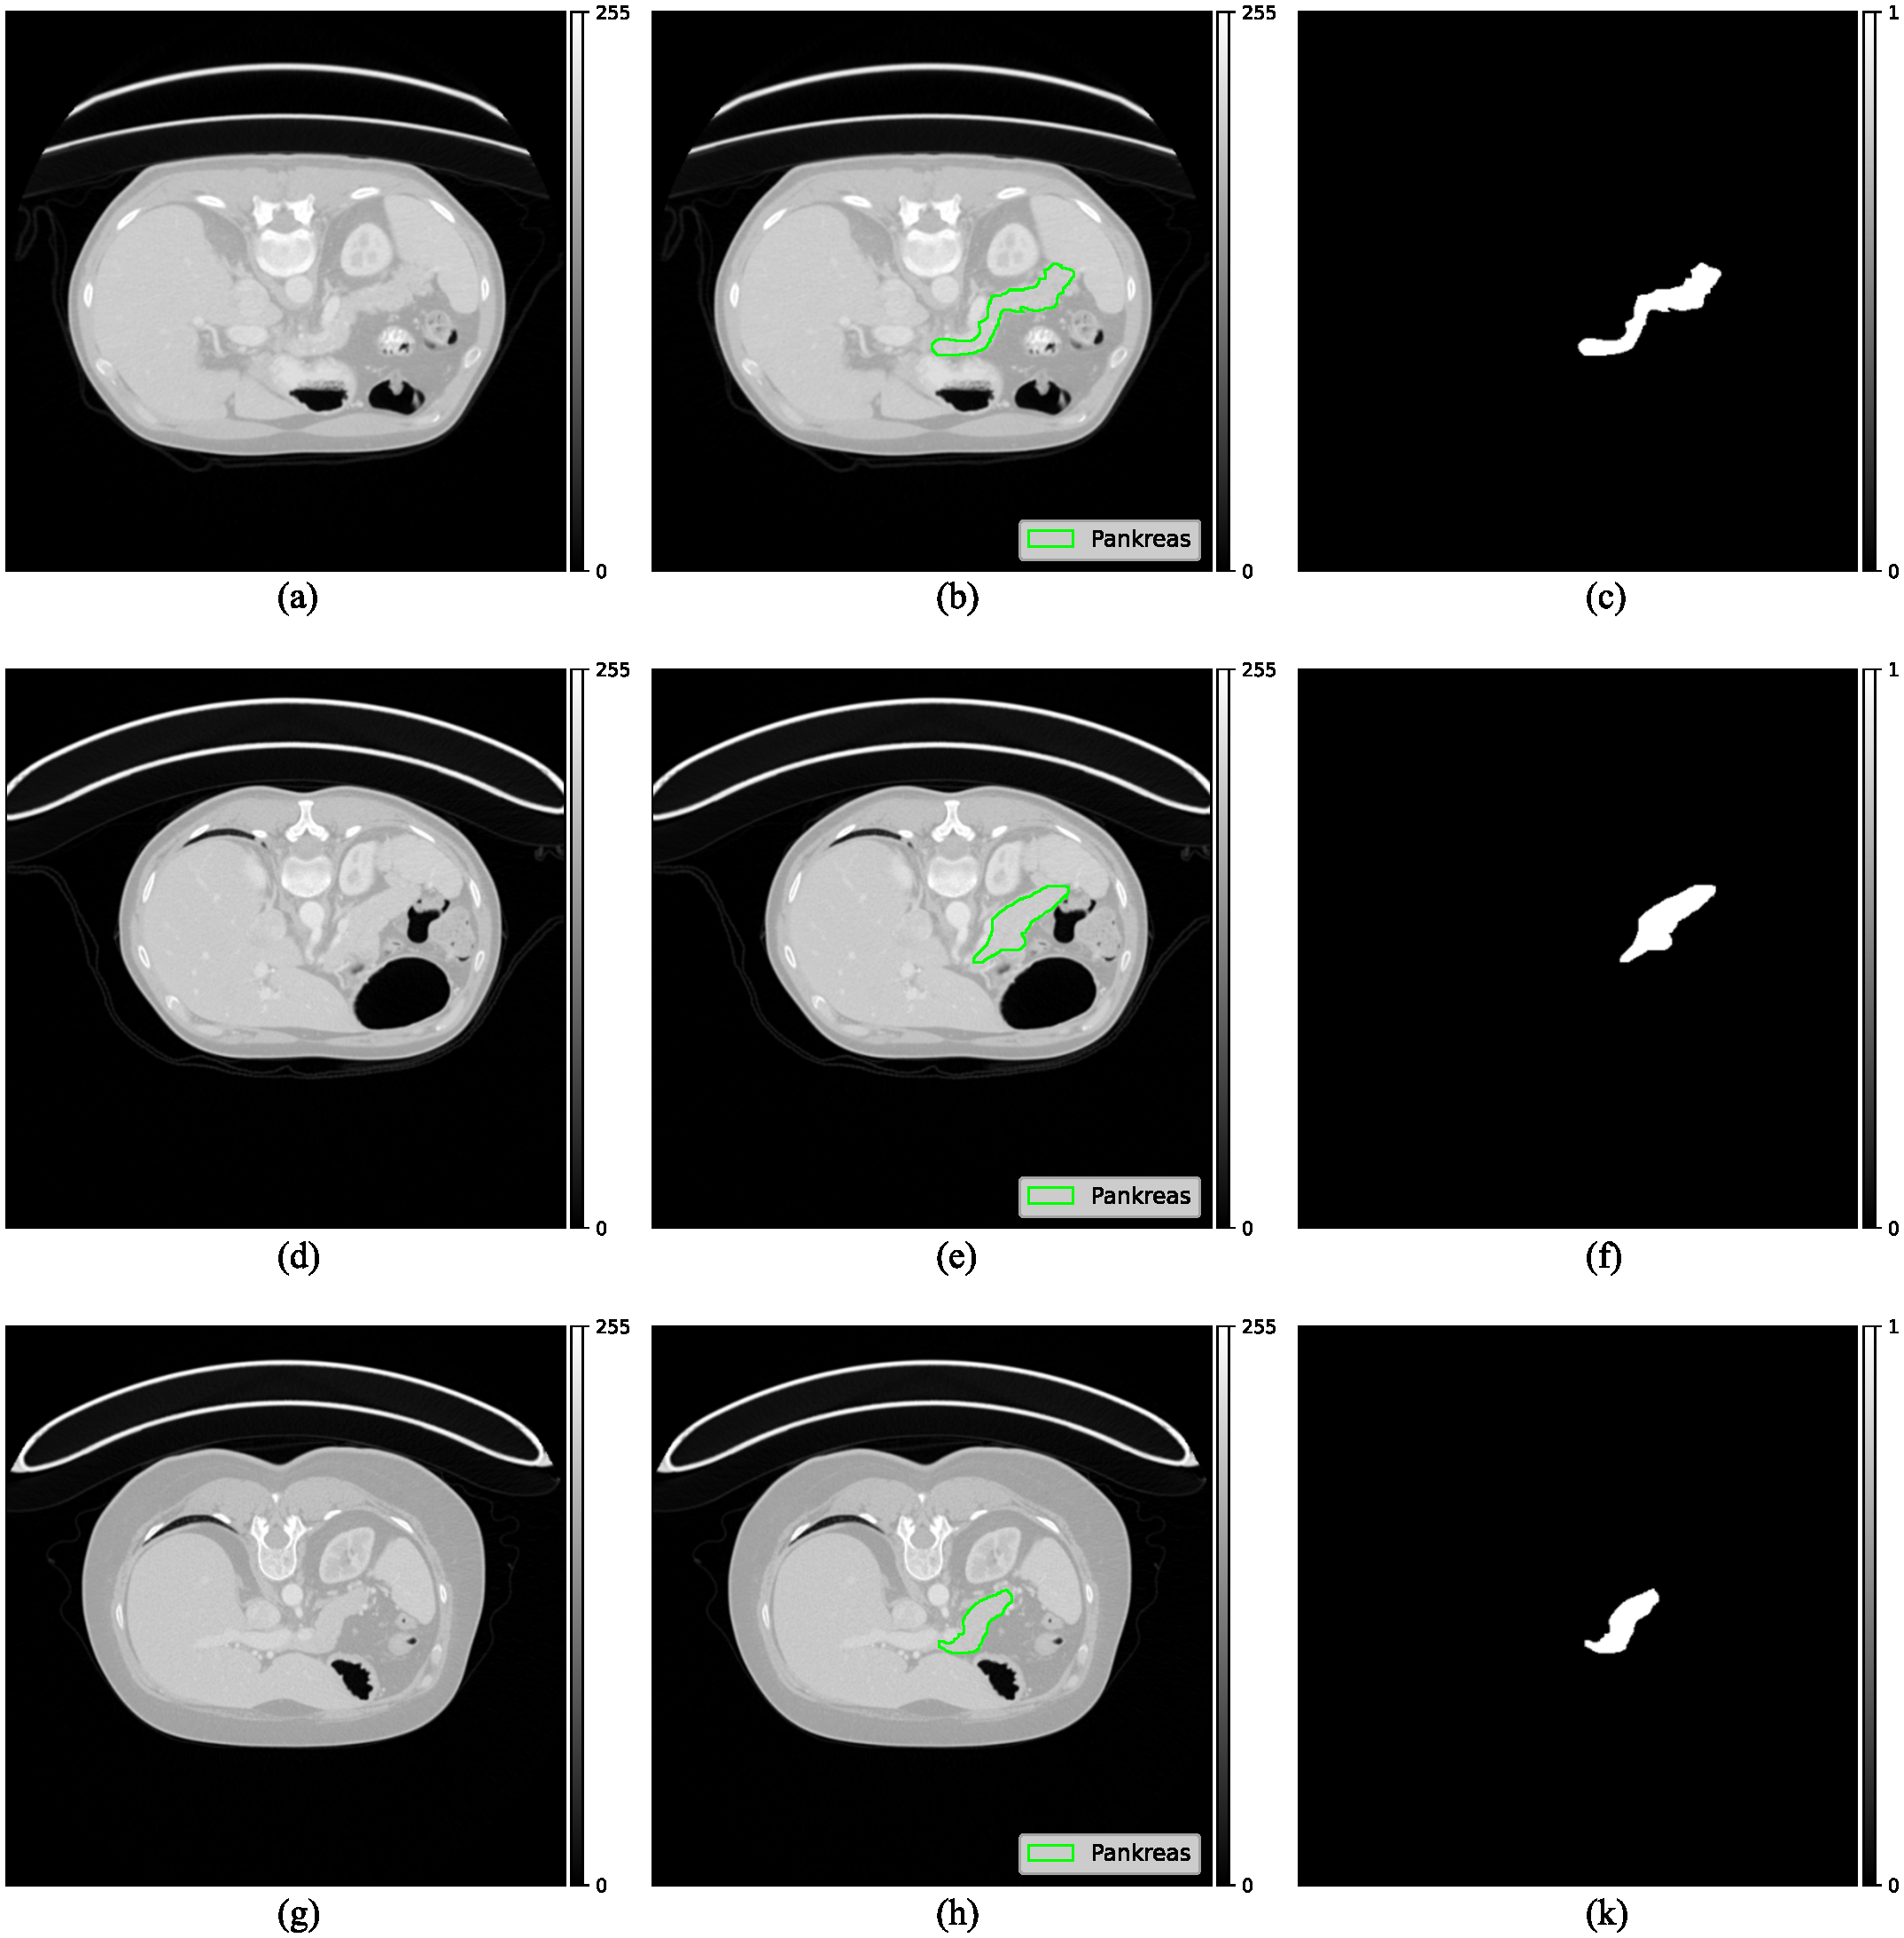
\includegraphics[scale=0.42]{Yapilan-Calismalar/Figures/nih_2dslices.pdf}
		}
	\end{center}
\end{figure} 

NIH veri setinde $82$ abdominal kontrastlı BT taraması ve ilgili taramalara ait BT dilimlerinin ayrı ayrı manuel olarak pankreas bölgeleri işaretlenmiş ikili (pankreas, diğer dokular) maskeleri bulunmaktadır. Her BT taramasındaki görüntülerin boyutu $512 \times 512 \times N$’dir. Burada $N$, BT taramalarındaki dilim sayısını ifade etmektedir. Veri setinde $N$ sayısı $181$ ile $466$ arasında değişmektedir. Veri seti oluşturulurken seçilen dilim kalınlığı $1,5$ mm ile $2,5$ mm arasında değişmektedir. Şekil \ref{fig:nih_2dslices}’da NIH pankreas veri setine ait bazı 2B görüntüler ile bu görüntülerin manuel olarak etiketlenmiş ikili maskeleri gösterilmektedir. BT taramalarındaki pankreas sınırları uzman doktorlar tarafından işaretlenmiştir. 

Tez çalışmasının ilk kısmında Pankreas İlgi Bölgesinin Belirlenmesi ve Pankreas Segmentasyonu fazlarının test ve eğitimi için NIH veri seti \%80 eğitim ve \%20 test olmak üzere iki parçaya ayrılmaktadır. Ayrıca, eğitim seti 4 rastgele gruba ayrılmakta ve 4-kat çapraz doğrulama gerçekleştirilmektedir. Üç set alt eğitim için, bir set ise validasyon için kullanılmaktadır. Alt eğitim ve validasyon seti, derin ağlarda parametre ayarlaması yapmak için kullanılmaktadır. En iyi ağ, sinir ağının eğitimi sırasında gerçekleştirilen validasyon ile elde edilen doğruluk ve hataya bağlı olarak belirlenmektedir. Ardından, önerilen ağının performansı test seti üzerinde ölçülmektedir.

\subsection{Tıbbi Bölütleme Dekatlon Veri Seti (Medical Segmentation Decathlon - MSD)}

Yapılan tez çalışmasının ikinci kısmında ilk kısımda önerilen iki aşamalı yöntemin 3 sınıflı (pankreas, pankreas tümörü, diğer dokular) kanser dokularının bulunduğu daha kompleks bir veri setinde performansı incelenmektedir. Bu kapsamda tez çalışmasının ikinci kısmında Tıbbi Bölümleme Decathlon Veri Seti (Medical Segmentation Decathlon - MSD) kullanılmaktadır. Bu veri seti  2018 yılında İspanya, Granada'daki Tıbbi Görüntü Hesaplama ve Bilgisayar Destekli Müdahaleler Konferansı (Medical Image Computing and Computer Aided Interventions Conference - MICCAI) sırasında kullanılmıştır \cite{simpson2019large}. 

BT taramalarındaki görüntüler Memorial Sloan Kettering Kanser Merkezi (New York, NY, ABD) tarafından sağlanmış ve daha önce radyomik uygulamalarda kullanılmıştır \cite{attiyeh2018survival,attiyeh2019preoperative,chakraborty2018ct}. Bu veri setindeki BT dilimleri DICOM formatında kaydedilmiştir. Bu veri setinde, kanserli organ segmentasyonu için kullanılabilecek $10$ farklı abdominal organdan çekilmiş BT taramaları mevcuttur. Bu organlar sırasıyla kalp, akciğer, hipokampus, prostat, akciğer, damar, dalak ve kolondur. Tez çalışması kapsamında gerçekleştirilen yaklaşımların değerlendirilmesi için MSD veri setinin pankreas ve pankreas tümörünü kapsayan alt veri seti kullanılmıştır. 

Pankreas veri seti, pankreas kitlelerinin (intraduktal müsinöz neoplazmalar, pankreas nöroendokrin tümörleri veya pankreas duktal adenokarsinomu) rezeksiyonu uygulanan hastalardan elde edilen BT taramalarından oluşmaktadır. Veri setinde $281$ abdominal kontrastlı BT taraması ve ilgili taramalara ait etiketler ile oluşturulmuş ikili maskeler bulunmaktadır. Her BT taramasındaki görüntülerin boyutu $512 \times 512 \times N$’dir. Burada $N$, BT taramalarındaki dilim sayısını ifade etmektedir. Veri seti oluşturulurken dilim kalınlığı $2,5$ mm olarak alınmaktadır. Şekil \ref{fig:msd_2dslices}’da Tıbbi Bölümleme Decathlon veri setine ait bazı 2B görüntüler ile bu görüntülerin manuel olarak etiketlenmiş ikili maskeleri gösterilmektedir. BT taramalarındaki pankreas sınırları uzman doktorlar tarafından işaretlenmiştir. Pankreas parankimi ve pankreas kitlesi (kist veya tümör), Scout uygulaması kullanılarak uzman bir abdominal radyolog tarafından her dilimde manuel olarak segmentlere ayrılmıştır \cite{hulovatyy2016scout}.

\captionsetup[figure]{margin={0.2cm,0cm}}
\begin{figure}[h!]
	\begin{center}
		\vspace{0.4cm}
		\captionbox{MSD pankreas veri setine ait örnek 2B BT dilimleri ile bu 2B dilimlerin manuel olarak etiketlenmiş ikili maskeleri.\label{fig:msd_2dslices}}
		{
			\vspace{0.4cm}
			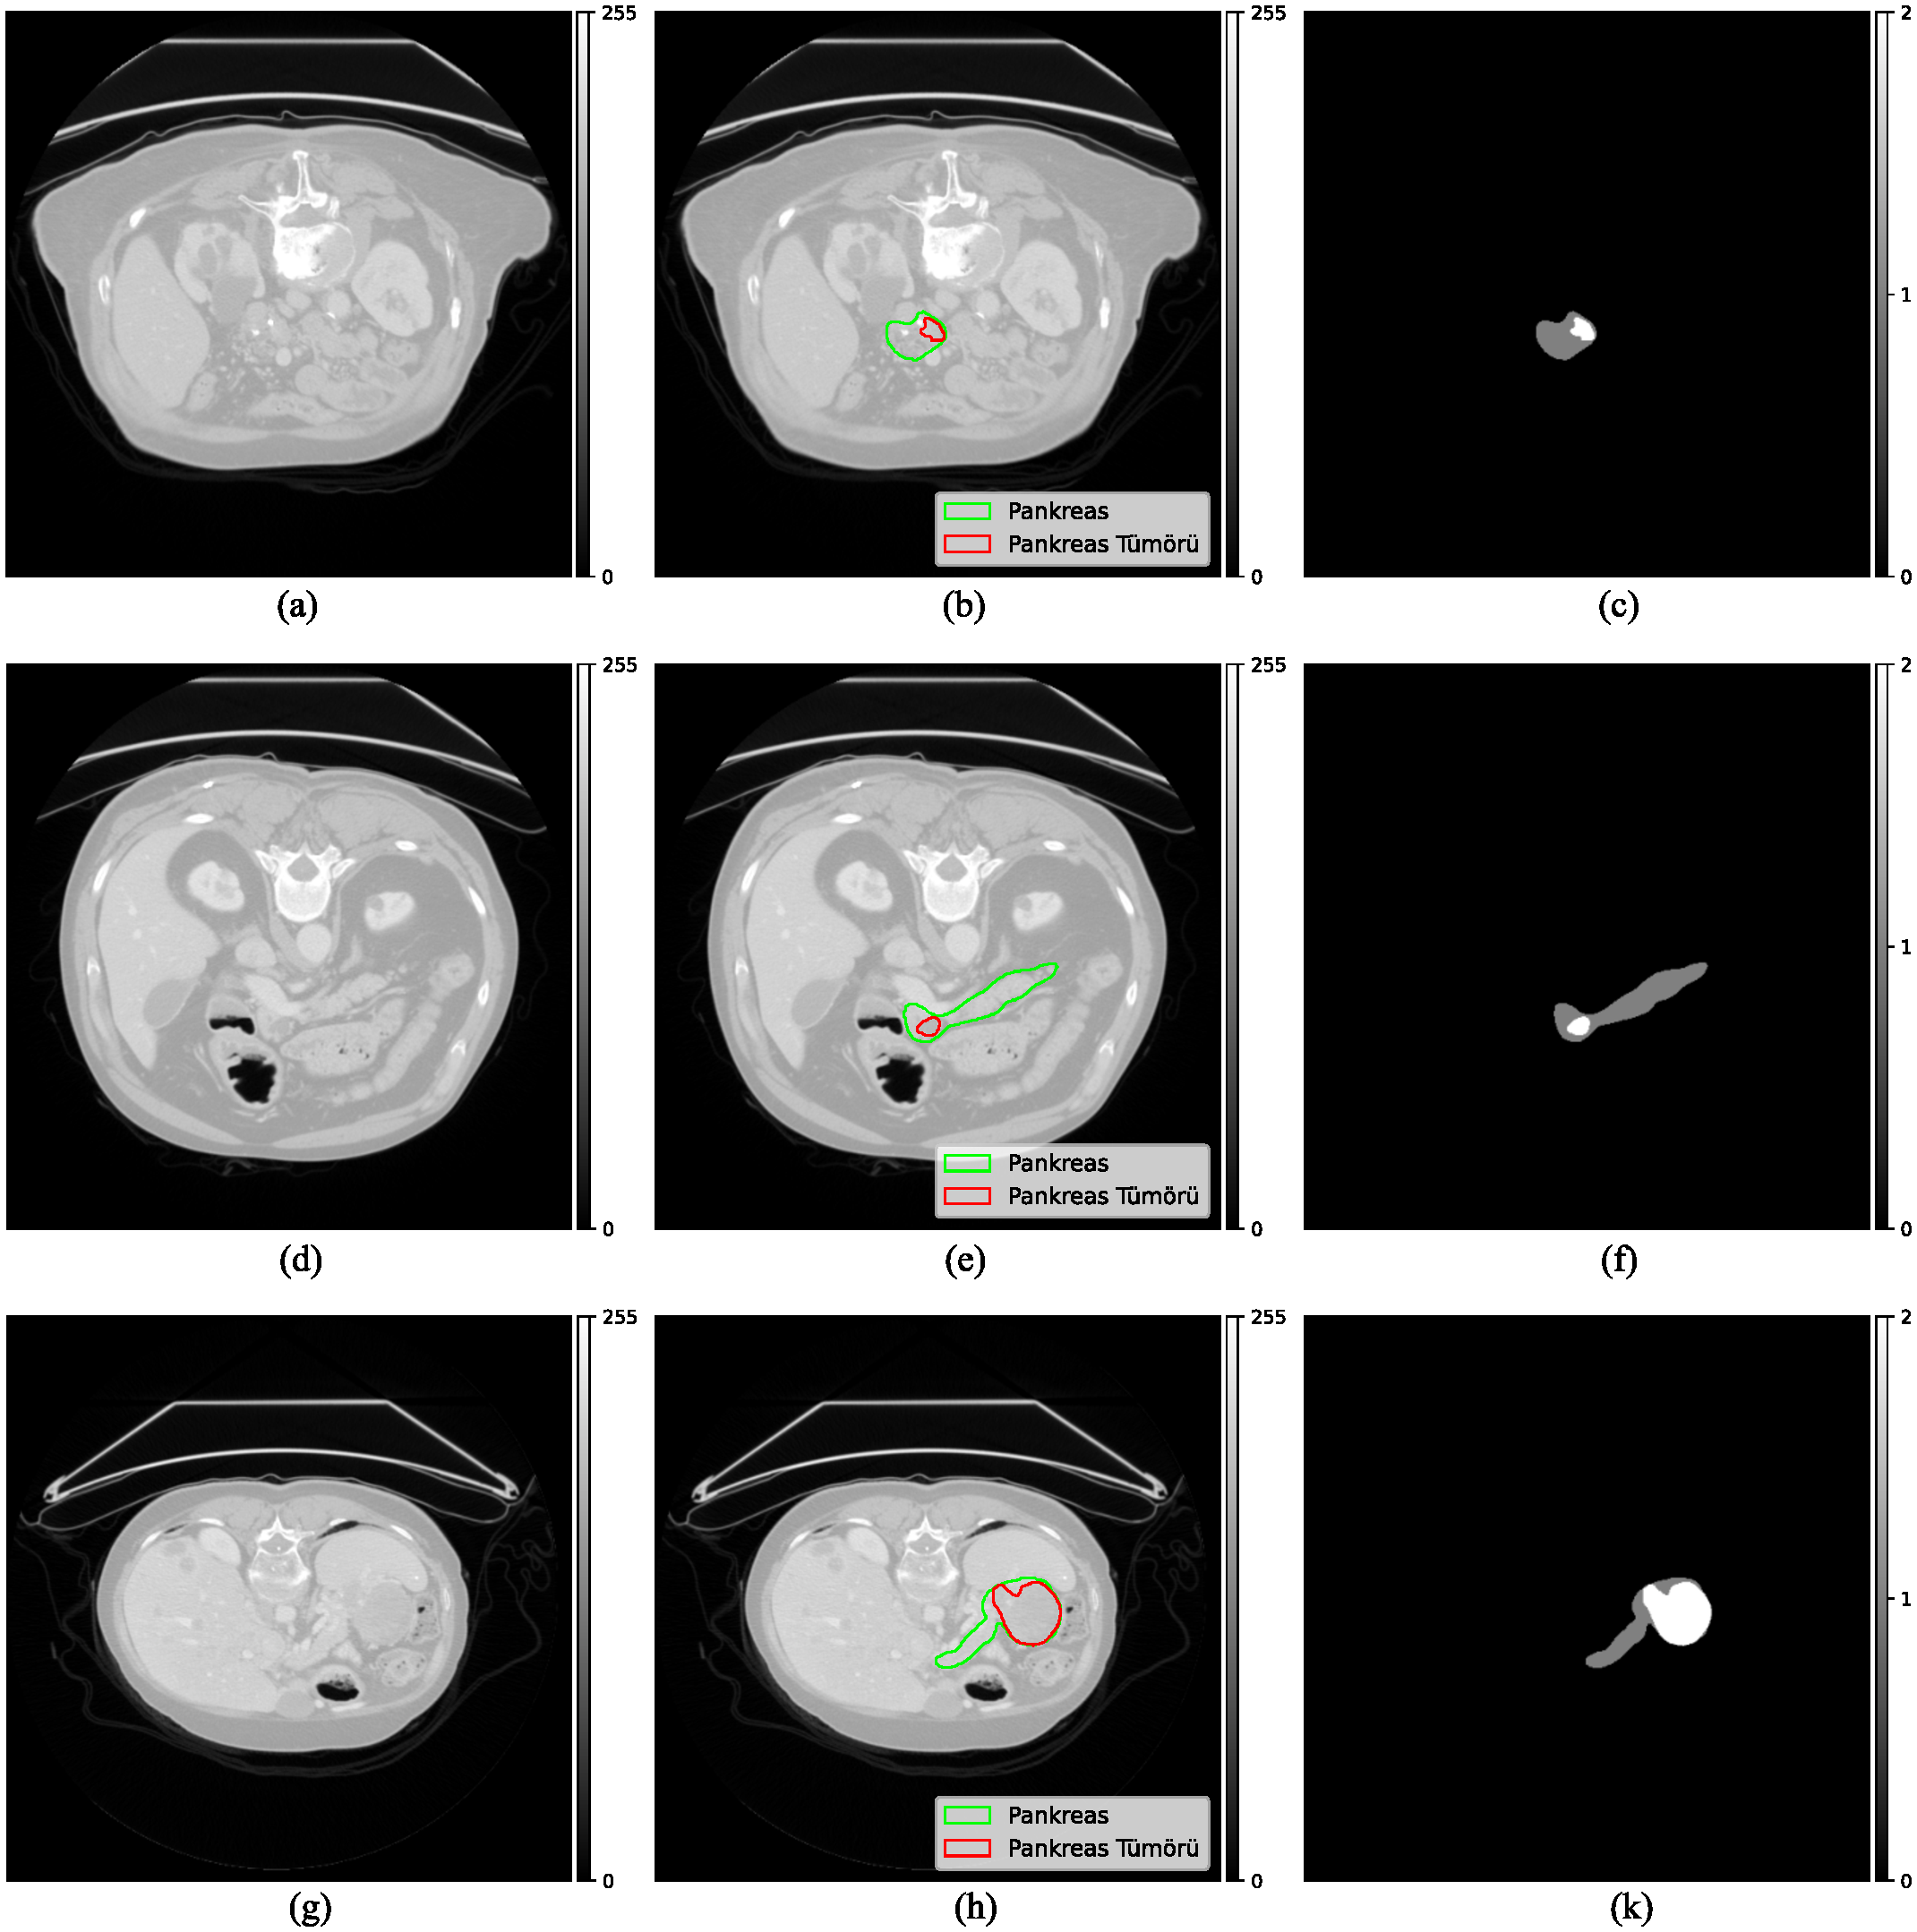
\includegraphics[scale=0.42]{Yapilan-Calismalar/Figures/msd_2dslices.pdf}
		}
	\end{center}
\end{figure} 

Tez çalışmasının ikinci kısmında Pankreas İlgi Bölgesinin Belirlenmesi ve Pankreas ve Pankreas Tümör Segmentasyonu fazlarının test ve eğitimi için Tıbbi Bölümleme Decathlon veri seti \%80 eğitim ve \%20 test olmak üzere iki parçaya ayrılmaktadır. Ayrıca, eğitim seti 4 rastgele gruba ayrılmakta ve 4-kat çapraz doğrulama gerçekleştirilmektedir. Üç set alt eğitim için, bir set ise validasyon için kullanılmaktadır. Alt eğitim ve validasyon seti, derin ağlarda parametre ayarlaması yapmak için kullanılmaktadır. En iyi ağ, sinir ağının eğitimi sırasında gerçekleştirilen validasyon ile elde edilen doğruluk ve hataya bağlı olarak belirlenmektedir. Ardından, çok katmanlı derin ağ mimarilerinin performansı test seti üzerinde ölçülmektedir.

\section{Performans Değerlendirme Metrikleri}
Tez çalışması kapsamında önerilen yaklaşımların değerlendirilmeleri için bilgisayarlı tomografi görüntülerinden oluşan ve farklı özelliklere sahip veri setleri kullanılmaktadır. Önerilen yaklaşımların performans analizleri elde edilen veri tabanları üzerinde gerçekleştirilen deneyler ile irdelenmekte ve literatürde var olan çalışmalara ait sonuçlarla kıyaslamaları gerçekleştirilmektedir. 

Çalışmada kullanılan performans değerlendirme metrikleri şu şekilde açıklanabilmektedir:

\begin{itemize}
	\item Dice Benzerlik Katsayısı (Dice Similarity Coefficient - DSC): Dice benzerlik katsayısı, el ile uzman kişi tarafından işaretlenmiş kesin referans bölgeler ile segment edilen bölgeler arasındaki benzerliği ölçmektedir \cite{dice1945measures}. Bu ölçüt Eşitlik \ref{eq:dsc_metric}’deki gibi hesaplanmaktadır.
	{\setlength{\mathindent}{0cm}
	\begin{equation}    
		\label{eq:dsc_metric}
		DSC=\frac{2 DP}{2 DP+YP+YN}
	\end{equation}}
	Eşitlik \ref{eq:dsc_metric}’de DP, YP ve YN sırasıyla, doğru pozitif, yanlış pozitif ve yanlış negatif sayılarını ifade etmektedir.
	
	\item Jaccard İndeksi (Jaccard Index - JI): Jaccard indeksi, uzman kişi tarafından manuel olarak tespit edilmiş kesin referans bölgelerle yaklaşım tarafından segment edilen bölgeler arasındaki benzerliği ölçmek için kullanılmaktadır \cite{jaccard1912distribution}. Bu değerlendirme prosedürü Eşitlik \ref{eq:ji_metric} kullanılarak temsil edilmektedir. 
	{\setlength{\mathindent}{0cm}
	\begin{equation}
		\label{eq:ji_metric}
		JI=\frac{DP}{DP+YP+YN}
	\end{equation}}
	Eşitlikte DP, YP ve YN sırasıyla, doğru pozitif, yanlış pozitif ve yanlış negatif sayısını temsil etmektedir. 
	
	\item Duyarlılık (Sensivity, Recall - REC): Duyarlılık performans değerlendirme metriği, segmentasyon yaklaşımı tarafından çıkarılan bölgenin piksel sayısının toplam piksel sayısına oranını göstermektedir \cite{altman1994diagnostic}. Bu değerlendirme metriği Eşitlik \ref{eq:rec_metric} kullanılarak elde edilmektedir.
	{\setlength{\mathindent}{0cm}
	\begin{equation}
		\label{eq:rec_metric}
		REC=\frac{DP}{DP+YN}
	\end{equation}}
	Eşitlikte DP ve YN sırasıyla, doğru pozitif ve yanlış negatif değerlerini temsil etmektedir.
	
	\item Özgüllük (Specificity - SPE): Özgüllük performans değerlendirme metriği, arka plan olarak segment edilen bölgenin piksel sayısının bölgenin toplam piksel sayısına oranını bulmak için kullanılmaktadır \cite{altman1994diagnostic}. Bu değerlendirme metriği Eşitlik \ref{eq:spe_metric} kullanılarak elde edilmektedir.
	{\setlength{\mathindent}{0cm}
	\begin{equation}
		\label{eq:spe_metric}
		SPE=\frac{DN}{DN+YP}
	\end{equation}}
	Eşitlikte DN ve YP sırasıyla, doğru negatif ve yanlış pozitif sayısını ifade etmektedir.
	
	\item Kesinlik (Precision - PRE): Kesinlik performans değerlendirme metriği, segmentasyon yaklaşımı tarafından çıkarılan bölgenin gerçekte ne kadar doğru olduğunu göstermekte kullanılmaktadır \cite{altman1994statistics}. Bu değerlendirme metriği Eşitlik \ref{eq:pre_metric} kullanılarak hesaplanmaktadır. 
	{\setlength{\mathindent}{0cm}
	\begin{equation}
		\label{eq:pre_metric}
		PRE=\frac{DP}{DP+YP}
	\end{equation}}
	Eşitlikte DP ve YP sırasıyla, doğru pozitif ve yanlış pozitif değerlerini temsil etmektedir.
	
	\item Doğruluk (Accuracy - ACC): Doğruluk performans değerlendirme metriği, segmentasyon yaklaşımı tarafından çıkarılan bölgenin piksel sayısının toplam piksel sayısına oranını göstermektedir \cite{metz1978basic}. Bu değerlendirme metriği Eşitlik \ref{eq:acc_metric} kullanılarak elde edilmektedir.
	{\setlength{\mathindent}{0cm}
	\begin{equation}
		\label{eq:acc_metric}
		ACC=\frac{DP+DN}{DP+DN+YP+YN}
	\end{equation}}
	Eşitlikte DP, DN, YP ve YN sırasıyla, doğru pozitif, doğru negatif, yanlış pozitif ve yanlış negatif sayısını temsil etmektedir.
	
	Yukarıdaki eşitliklerde DP (Doğru Pozitif) doğru olarak segmentlere ayrılmış bölgeyi, YP (Yanlış Pozitif) yanlış segmentlere ayrılmış bölgeyi ve YN (Yanlış Negatif) eksik olarak segmentlere ayrılmış bölgeyi temsil etmektedir.
	
	\item Alıcı Çalışma Karakteristikleri (Receiver Operating Characteristics - ROC) Eğrisi: ROC eğrisi performans değerlendirme metriği, uzman kişi tarafından manuel olarak tespit edilmiş kesin referans bölgelerle yaklaşım tarafından segment edilen bölgeler arasındaki benzerliği ölçmek için kullanılmaktadır \cite{metz1978basic,fawcett2006introduction}. Segmentasyon yaklaşımının ROC eğrisini çizmek için Spesifiklik (Yanlış Pozitif oranı) ve Duyarlılık (doğru pozitif oranı) olmak üzere iki metrik gerekmektedir.
	
	\item ROC Eğrisinin Alt Alanı (Area under the ROC Curve – AUC): AUC, ROC eğrisinin üzerindeki alanlar ile ROC eğrisinin altındaki alanlar arasındaki farkı ifade etmektedir \cite{hanley1982meaning}. Bu değerlendirme metriği Eşitlik \ref{eq:auc_metric} kullanılarak elde edilmektedir.
	{\setlength{\mathindent}{0cm}
	\begin{equation}
		\label{eq:auc_metric}
		AUC=\int_{x}^{y} f(i) d_{i}
	\end{equation}}
	Eşitlik \ref{eq:auc_metric}'de $f(i)$ ROC eğrisinin üstünde ve altındaki alanları temsil eden bir fonksiyondur. '$x$' ve '$y$', ROC eğrisindeki minimum ve maksimum eksen noktalarını ifade etmektedir.	
\end{itemize}

İdeal pankreas ve pankreas tümör segmentasyonu yaklaşımı ile elde edilen DSC, JI, PRE, REC, ACC, SPE ve AUC değerlerinin diğer yaklaşımlardan daha yüksek olması beklenmektedir.

\section{Literatür Çalışmaları}

Bu tez çalışmasında öncelikle sadece pankreas verilerinin manuel işaretli olduğu NIH veri seti kullanılarak pankreas segmentasyonunun gerçekleştirilmesine yönelik bir yöntem önerilmektedir. Daha sonra pankreas ve pankreas tümör dokularının ayrı ayrı işaretli olduğu MSD veri seti üzerinde farklı derin öğrenme modelleri kullanılarak önerilen yöntemin performansında iyileştirmeler gerçekleştirilmektedir.

Yapılan tez çalışmasının ilk kısmı olan otomatik pankreas segmentasyonu yıllardır aktif olarak çalışılan alanlardan biridir. Bu alan için literatürde birçok çalışma geliştirilmiştir. Bu çalışmalar kronolojik sıraya göre bölge temelli, atlas temelli, model temelli ve derin öğrenme temelli olmak üzere 4 ana grupta ele alınmaktadır. Günümüzde pankreas ve pankreas tümör dokularının segmentasyonuna yönelik çalışmalar derin öğrenme temelli yöntemlerin güçlü segmentasyon sonuçları üretebilmesinden dolayı genellikle derin öğrenme ile gerçekleştirilmektedir.

\subsection{Pankreas Segmentasyonu İçin Kullanılan Bölge Temelli Çalışmalar}

Bölge temelli segmentasyon yaklaşımı en popüler algoritmalardan biridir. Bu çalışmalarda tüm piksellerin anlamlı bölgeleri çıkarılmaktadır. Bölge temelli çalışmalar dört kategoriye ayrılabilmektedirler: 

\begin{enumerate}
    \item Bölge Büyütme Yöntemi: Bu yöntem basitliği ve iyi performansı nedeniyle segmentasyon için en popüler tekniklerden biridir. Çalışma prensibi, bir noktadan başlayarak, komşu piksellerin homojenliği temelinde bir bölge büyütmek, homojen ve bağlantılı bir bölge elde edilene kadar tüm süreci yinelemektir. 2015 yılında Tam ve Nguyen, pankreası BT görüntülerinden segmentlere ayırmak için bölge büyütme ve histogram eşitleme tekniklerini kullanmakta ve Jaccard indeksini 86.87 ile oldukça yüksek sonuçlar elde etmektedirler \cite{tam2014efficient}.

Avantajları: Bağlantılı bölgeler garanti edilmektedir. 

Dezavantajları: Başlangıç noktasını elde etmek için manuel etkileşim gerektirmekte ve aşırı segmentasyona neden olan gürültüye duyarlıdır. 

    \item Böl ve Birleştir Yöntemi: Bu yöntem görüntünün tamamı üzerinde çalışmakta ve homojenliği ayırt etmek için dörtlü ağaç verilerini kullanmaktadır. İşlem süreci, görüntünün tamamının rastgele bağlantısız alt bölgelere bölünmesi ve ardından bu alt bölgelerin makul görüntü bölümlendirme koşulu temelinde birleştirilmesidir. Pankreas segmentasyonu için, bölge ayırma ve birleştirmeye dayalı yöntem tatmin edici segmentasyon sonuçları elde edememektedir \cite{farag2017automatic}. 

    Avantajları: Bağlantılı bölgeler garanti edilmektedir. 

    Dezavantajları: Görüntünün konumu ve yönü, bloklu son segmentasyona yol açmaktadır.
    
    \item Kümeleme Yöntemi: Bu yöntem daha klasik ve yaygın olarak kullanılmaktadır. Temel amacı, aynı özelliklere sahip piksellere benzemektir. K-ortalama kümeleme, nokta değeri ile bu kümenin ortalama değeri arasındaki farkın en küçük olduğu kümeye p noktası ekleyerek tüm görüntüyü k kümeye veya gruba bölmektedir.

    Avantajları: Basit ve kullanışlıdır, genellikle tıbbi görüntüleme ve güvenlik sistemleri için geçerlidir.

    Dezavantajları: K-ortalama kümeleme gibi bazı kümeleme algoritmaları, sürekli bölgeyi garanti edememektedir. 

    \item Eşikleme Yöntemi: Bu yöntem bölütlenecek nesneyi (ön planı) arka plandan ayırmak için görüntünün histogram gibi global bilgilerini kullanmaktadır. 
    
    Avantajları: Basit ve kullanışlıdır.

    Dezavantajları: Eşiği tam olarak belirlemek zordur. 

\end{enumerate}


\subsection{Pankreas Segmentasyonu İçin Kullanılan Atlas Temelli Çalışmalar}
Bu teknikler görüntülerde pankreas varlığı hakkında ön fikir veren bir harita oluşturmaktadır. Araştırmacılar bu çalışmalarda pankreasın bölge ve boyutunu kestirmek için regresyon ormanı yöntemi \cite{oda2016regression}, ağırlıklı alt uzaysal olasılık atlasları \cite{karasawa2015pancreas}, yapıya özel atlas üretimi \cite{karasawa2015pancreas},  pankreas dokusu çevresindeki damar yapısına dayanan atlas seçim stratejisi \cite{karasawa2017multi}, atlas seçimi ve grafik kesime dayalı yöntem \cite{oda2011organ}, mekansal olarak bölünmüş olasılık atlaslarına dayanan otomatik yöntem \cite{chu2013multi}, hiyerarşik atlas kaydı ve ağırlıklandırma şemasına dayanan yöntem \cite{wolz2013automated}, segmentasyon doğruluğuna ve etkileşim maliyetlerine dayalı yöntem \cite{takizawa2017interactive}, hastaya özel olasılık atlas rehberli segmentasyon yöntemi \cite{shimizu2010automated}, koşullu şekil -- konum ve denetimsiz yoğunluk öncelikleri temelli yöntem \cite{okada2015abdominal} geliştirmişlerdir. Bu tekniklerin en kritik dezavantajlarından biri hesaplama maliyetinin oldukça yüksek olmasıdır.

\subsection{Pankreas Segmentasyonu İçin Kullanılan Model Temelli Çalışmalar}
Bu teknikler pankreasın segmentasyonu için pankreas istatistiksel şekil modelini uyarlamaktadırlar \cite{hammon2013model}.  Pankreasın farklı anatomik yapısı nedeniyle, bu teknikler tatmin edici sonuçlar verememektedirler.

\subsection{Pankreas Segmentasyonu İçin Kullanılan Derin Öğrenme Temelli Çalışmalar}
Derin Sinir Ağları (Deep Neural Network - DNN) tabanlı tekniklerde pankreastaki etkin özellikler doğrudan görüntü verilerinden elde edilmektedir. Derin sinir ağlarının hızla gelişmesi ile sınıflandırma \cite{roth2015deep,roth2015deeporgan}, lokalizasyon \cite{roth2016spatial,roth2018spatial}, tanıma \cite{zhou2016pancreas,cai2017improving}, segmentasyon \cite{yu2018recurrent,ma2018novel,zhu20183d} ve hizalama \cite{roth2015deeporgan,chen2019harnessing} gibi birçok tıbbi görüntü işleme ve bilgisayarla görme uygulamalarında tatmin edici performanslar elde edilmektedir. Bunun üzerine araştırmacılar derin öğrenme (DÖ) yöntemlerini kullanarak pankreas segmentasyonu için daha yüksek doğruluklu sonuçlar elde etmeye başlamışlardır. Otomatik pankreas segmentasyonu için DÖ yöntemlerini kullanan literatür çalışmaları pankreas segmentasyonu başarısını önemli ölçüde artırmıştır. Son yıllarda pankreas segmentasyon başarısının artması ile derin öğrenme temelli yaklaşımlar pankreas tümör segmentasyonunda da kullanılmaya başlanmıştır. Bu amaçla 3 sınıflı (Pankreas, Pankreas Tümörü, Diğer dokular) MSD gibi veri setleri araştırmacıların açık erişimine açılmıştır.

\subsubsection{Sadece Pankreas Organının Segmentasyonuna Yönelik Gerçekleştirilen Derin Öğrenme Temelli Akademik Çalışmalar}
Bu tez çalışmasında pankreas segmentasyonu için iki aşamalı derin öğrenme esaslı bir yöntem önerilmiştir. Bu çalışmada kullanılan derin öğrenme tekniklerini kullanarak pankreas segmentasyonu gerçekleştiren benzer çalışmalar ve bu çalışmaların başarıları Tablo \ref{tab:lit1}'deki gibi özetlenebilmektedir.

\begin{table}[h!]
	\centering
	\caption{Otomatik pankreas segmentasyonu için derin öğrenme yöntemlerini kullanan literatür çalışmaları}
	\label{tab:lit1}
	\begin{tabular}{cccccc}
		\toprule
		Metot                           &  Veri Seti   &  Model              & Başarı (DSC\%)  \\ 
		\midrule 
		Roth 2015 - 1 \cite{roth2015deep}  &  NIH-82    &  Hierarchical Coarse-to-Fine          & 68$\pm$10   \\ 
		Roth 2015 - 2 \cite{roth2015deeporgan}  &  NIH-82    &  ConvNets                             & 71,8$\pm$10,7 \\
		Roth 2016     \cite{roth2016spatial}    &  NIH-82    &  Holistically Nested Network          & 78,01$\pm$8,2 \\
		Roth 2018     \cite{roth2018spatial}    &  NIH-82    &  Holistically Nested Network          & 81,27$\pm$6,27\\
		Zhou 2016     \cite{zhou2016pancreas}    &  NIH-82    &  Coarse-to-Fine                       & 82,37$\pm$5,68\\
		Cai 2017      \cite{cai2017improving}     &  NIH-82    &  Recurrent Neural Contextual Learning & 82,4$\pm$6,7 \\
		Yu  2017      \cite{yu2018recurrent}      &  NIH-82    &  Saliency Transformation Network      & 84,5$\pm$4,97 \\
		Ma 2018       \cite{ma2018novel}      &  NIH-82    &  Bayesian Model                      & 85,32$\pm$4,19 \\
		Zhu 2018      \cite{zhu20183d}     &  NIH-82    &  3D Coarse-to-Fine                   & 84,59$\pm$4,86 \\
		Zhao 2019     \cite{zhao2019fully}    &  NIH-82    &  3D U-Net                             & 85,99$\pm$4,51 \\
		Chen 2019     \cite{chen2019harnessing}    &  NIH-82    &  3D Coarse-to-Fine                   & 85,22$\pm$4,07 \\
		Khosravan 2019\cite{khosravan2019pan}& NIH-82    &  Projective Adversial Network        & 85,53$\pm$1,23 \\
		Li 2019       \cite{li2020model}       &  NIH-82    &  Model Driven Stack - based FCN      & 83,5$\pm$6,2  \\
		Xue 2019       \cite{xue2019cascaded}     &  NIH-82    &  Cascaded 3D FCN      & 85,9$\pm$5,1  \\	
		Liu 2019       \cite{liu2019automatic}     &  NIH-82    &  Ensemble-based FCN  & 84,10$\pm$4,91  \\		 
		Zheng 2020     \cite{zheng2020deep}  &  NIH-82    &  2D U-Net      & 84,37 \\	 
		Zhou 2017    \cite{zhou2017deep}     &  JHMI      &  Deep Supervision  & 79,23$\pm$27,71   \\
		Zhu 2018      \cite{zhu20183d}      &  JHMI      &  3D Coarse-to-Fine & 80,56$\pm$13,36   \\
		\bottomrule
	\end{tabular}
\end{table}

Pankreas segmentasyonu için popüler derin öğrenme ağ modellerinde sıklıkla kullanılan konvolüsyon katmanlarını kullanan ilk çalışma Roth tarafından geliştirilmiştir \cite{roth2015deep}. Bu çalışmada NIH pankreas veri seti oluşturulmuş ve yerel görüntü bölgeleri (pankreas) Hiyerarşik Kabadan İnce (Hierarchical Coarse-to-Fine) modele dayanan bir yöntem kullanılarak sınıflandırılmıştır. Daha sonra Roth, 2B görüntü dizilerindeki pikselleri piksel başına maskeleme aracılığıyla bağımsız olarak işleyen Holistik İç İçe Evrişimsel Sinir Ağları (Holistically-Nested Convolutional Neural Networks) ile pankreas segmentasyon performansını geliştirmiştir \cite{roth2016spatial,roth2018spatial}. Zhou, Kabadan İnceye (Coarse-to-Fine) yaklaşımıyla pankreas segmentasyonu gerçekleştiren bir çalışma geliştirmiştir \cite{zhou2016pancreas}. Bu yaklaşımda öncelikle kaba ölçekli faz ile kaba olarak pankreas bölgesi çıkarılmaktadır. Daha sonra ince ölçekli fazda bu kaba bölgeler tekrar sınıflandırılarak detaylı pankreas bölgesi elde edilmektedir. Performans bakımından yeterli olsa da, kaba ve ince ölçekli fazların ayrı ayrı eğitimi ve test edilmesi nedeniyle daha yüksek hesaplama maliyeti gibi bazı dezavantajları mevcuttur. Bağlamsal öğrenme ve segmentasyonun tutarlılık sorununu çözmek için Cai, Bağlamsal Tekrarlayan Sinir Ağları (Contextual Recurrent Neural Networks: CRNN) yaklaşımını önermiştir \cite{cai2017improving}. Yu, kaba ve ince ölçekli fazları Belirgin Dönüşüm Ağı (Saliency Transformation Network) aracılığıyla birbirine bağlayarak Zhou tarafından önerilen \cite{zhou2016pancreas} önceki yaklaşımın performansını geliştirmiştir \cite{yu2018recurrent}. Ma, derin sinir ağı ve istatistiksel şekil modelinin segmentasyon sonuçlarının birleştirildiği Bayes modeline dayanan hibrit bir yaklaşım önermiştir \cite{ma2018novel}. 

Literatür çalışmalarında, 2B CNN’ye dayalı tekniklerin BT’nin üçüncü boyuttaki bilgilerinin elde edilmesinde kısıtlamalara sahip olduğu bildirilmektedir. Bu nedenle, 2B ağlara göre önemli ölçüde daha yüksek hesaplama gücü ve bellek gerektiren 3B ağlar kullanılarak (3B U-Net \cite{zhao2019fully}, 3B Kabadan İnceye (3D Coarse-to-Fine) \cite{zhu20183d,chen2019harnessing}, 3B Tamamen Konvolüsyonel Ağlar (Fully Convolutional Networks : FCN) \cite{roth2018application}, Projektif Çekişmeli Ağlar (Projective Adversarial Networks : PAN) \cite{khosravan2019pan}, Kaskat 3B FCN (Cascaded 3D FCN) \cite{xue2019cascaded}) daha yüksek başarıya sahip pankreas segmentasyon sonuçları elde edilmiştir. 

Pankreas segmentasyonu ile ilgili literatür çalışmalarını test etmek için kullanılan bir başka veri seti JHMI patolojik kist veri setidir \cite{zhu20183d,zhou2017deep}. Fakat bu veri seti ilgili araştırmacılar tarafından serbest kullanım için henüz paylaşılmamıştır. Tablo \ref{tab:lit1}’de gösterilen literatür çalışmalarının başarılarına göre, NIH ve JHMI veri setleri için maksimum Dice Benzerlik Katsayısı (Dice Similarity Coefficient - DSC) değerleri 3B U-Net \cite{roth2015deep, farag2016bottom} ve 3B Kabadan İnceye (3D Coarse-to-Fine) \cite{zhu20183d}'de elde edilen \%85.99 ve \%80.56 değerleridir. Bu çalışmalar önceki çalışmalara göre \%17.99 ve \%1.33 iyileştirme sağlamışlardır.

\subsubsection{Pankreas ve Pankreas Tümörü Segmentasyonu İçin Gerçekleştirilen Derin Öğrenme Temelli Akademik Çalışmalar}

Tez çalışmasının ikinci kısmı otomatik pankreas ve pankreas tümör segmentasyonudur. Pankreas ve pankreas tümörünün değişken büyüklüğü, şekli ve konumu nedeniyle literatürde bu alanla ilgili çok çalışma bulunmamaktadır. Yapılan çalışmalar da belirli bir başarı yüzdesine kadar ulaşabilmektedirler. Otomatik pankreas ve pankreas tümörü segmentasyonu için DÖ yöntemlerini kullanan literatür çalışmaları Tablo \ref{tab:lit2}’te listelenmektedir. Bu çalışmalar şu şekilde özetlenebilmektedir: 

\begin{table}[h!]
	\centering
	\caption{Otomatik pankreas ve pankreas tümör segmentasyonu için derin öğrenme yöntemlerini kullanan literatür çalışmaları}
	\label{tab:lit2}
	\begin{adjustbox}{width=\textwidth}
	\begin{tabular}{ccm{5cm}cccc}
		\toprule
		Metot                           &  Veri Seti   &  Model  & Pankreas (DSC\%)  & Tümör (DSC\%) \\ 
		\midrule 
		Isense 2018 \cite{isensee2018nnu}  &  MSD    &  nnU-Net (no-new-Net)  & 79,53 & 52,27  \\ 
		Cai 2019 \cite{cai2019end}  &  MSD   &  Adversarial Shape Learning & 74,3$\pm$12,2 & - \\
		Xia 2020 \cite{xia2020uncertainty}    &  MSD    &  Uncertainty-awere Multi-view Co-training (UMCT)   & 74,93 & - \\
		Yu 2020 \cite{yu2020c2fnas}    &  MSD    & Corse-to-Fine Neural Architecture Search (C2FNAS)   & 80,76 & 54,41\\
		Yu 2021 \cite{yu2020cakes}    &  MSD    & Channel-wise Automatic Kernel Shirinking (CAKES) & 80,12 & 48,72\\
		Zhu 2019 \cite{zhu2019v}     &  MSD    &  V-NAS & 79,94$\pm$8,85 & 37,78$\pm$32,12 \\
		Tureckova 2020 \cite{tureckova2020improving}      &  MSD    &  Deep Supervision and Atentional Gates      & 81,81$\pm$0,98 & 52,68$\pm$1,89 \\
		Xia 2020       \cite{xia20203d}      &  MSD    &  3D Semi Supervised Learning                      & 78,42 & 38,48 \\
		\bottomrule
	\end{tabular}
	\end{adjustbox}
\end{table}

2015 yılında sunulan U-Net, sade ve başarılı yapısı ile tıbbi görüntü segmentasyonunda hızla yaygın olarak kullanılan bir mimari haline gelmiştir. Bununla birlikte, U-Net'in yeni problemlere uyarlanması, kesin mimari, ön işleme, eğitim ve çıkarımla ilgili birkaç serbestlik derecesini içermektedir. Bu seçenekler birbirinden bağımsız olmayıp genel performansı önemli ölçüde etkilemektedir. Isensee çalışmasında U-Net’in bu eksikliklerini minimize etmek amacıyla nnU-Net (no-new-Net)’i önermiştir \cite{isensee2018nnu}. Bu modelde 2B ve 3B U-Net modellerinin temel yapıları birleştirilmektedir. Önerilen bu model, pankreas ve pankreas tümör BT dilimlerini içeren Decathlon veri seti kullanılarak değerlendirilmiştir. 

Karın (abdomel) organlarının genelde şekil ve topolojilerinin farklı olmasından dolayı geleneksel CNN tabanlı segmentasyon modellerini eğitmek zor olmaktadır. Cai çalışmasında bu dezavantajı minimize etmek için Uçtan Uca ve Şekil öğrenme (Adversarial Shape Learning) mimarili yeni bir model önermiştir \cite{cai2019end}. Model girdi olarak derin öğrenme özelliklerini almakta ve organ yüzeyinde bulunan noktalar olarak organ şekli temsillerini üretmektedir. Ek olarak bu çalışmada şekil bilgilerini daha iyi yakalamak ve nokta ağını optimize etmek için yeni bir çekişmeli şekil öğrenme amaç fonksiyonu sunulmaktadır.

Segmentasyon uygulamalarında performansı en üst düzeye çıkarmak için değişen model topolojileri, optimizasyon parametreleri, ön işleme adımları ve model topolojileri geliştirmek standart uygulamalardandır. Fakat bu standart uygulamaların farklı görevlere nasıl aktarıldığı genellikle net değildir. Bu durumu ortadan kaldırmak amacıyla, Perslev çalışmasında tıbbi görüntülerin segmentasyonu için basit ve kapsamlı derin öğrenme modeli önermiştir \cite{perslev2019one}. 

Tıbbi görüntü segmentasyonunda büyük başarı elde etmiş olsa da, derin öğrenmeye dayalı yaklaşımlar genellikle tıbbi görüntü analizi alanında son derece pahalı olabilen, büyük miktarda ve iyi açıklamalı veri gerektirmektedir. Öte yandan, etiketlenmemiş verilerin elde edilmesi çok daha kolaydır. Yarı denetimli öğrenme ve denetimsiz alan uyarlaması, birbirleriyle yakından ilişkili olup etiketlenmemiş verilerden yararlanmaktadır. Xia çalışmasında tıbbi görüntü segmentasyonu (pankreas segmentasyonu) için bu iki görevi ele alan ve birleşik çerçeve olan Belirsizliğe Duyarlı Çoklu Görüş Ortak Eğitimi (Uncertainty-aware Multi-view Co-training  - UMCT) önermiştir \cite{xia2020uncertainty}. Önerilen yöntem daha iyi performans için etiketlenmemiş verileri verimli bir şekilde kullanma yeteneğine sahiptir.

Literatürde 3B konvolüsyonel sinir ağlarının 3B tıbbi görüntülerde organları veya tümörleri ayrıştırmada çok başarılı olduğu kanıtlanmıştır. Ancak farklı görev bağlamları verilen uygun 3B ağları seçmek veya tasarlamak karmaşık ve zaman alıcı olmaya devam etmektedir. Son zamanlarda, en iyi ağ mimarisini otomatik olarak arayarak bu sorunu çözmek için Yapay Mimari Arama (Neural Architecture Search - NAS) algoritmaları önerilmektedir. Yu çalışmasında, ağ boyutu veya giriş boyutunda tutarsızlık olmadan 3B segmentasyon ağını sıfırdan otomatik olarak aramak için Kabadan İnceye Sinir Mimari Araması (Coarse-to-Fine Neural Architecture Search - C2FNAS) önermiştir \cite{yu2020c2fnas}.

3B CNN video analizi ve hacimsel görüntü tanıma gibi 3B sahne anlamada yaygın olarak uygulanmaktadır. Fakat, 3B ağlar pahalı hesaplama maliyetine neden olan aşırı parametrelendirmeye kolayca yol açabilmektedirler. Yu çalışmasında, standart 3B konvolüsyonları bir dizi operasyonla küçülterek verimli 3B öğrenmeyi mümkün kılmak için Kanal Otomatik Çekirdek Küçültmesini (Channel wise Automatic KErnel Shrinking - CAKES) önermiştir \cite{yu2020cakes}.

Derin Öğrenme sistemlerinin güvenilirliği doğruluklarına değil, aynı zamanda girdi verilerindeki olumsuz bozulmalara karşı sağlamlıklarına da bağlıdır. Daza çalışmasında doğal görüntü alanındaki olumsuz gürültü varlığında Derin Sinir Ağlarının performansını iyileştirmek için çeşitli saldırılar ve savunmalar önermiştir \cite{daza2021towards}. Bununla birlikte, bu çalışmada hacimsel veriler için bilgisayar destekli tanılamadaki sağlamlık, yalnızca belirli görevler için ve sınırlı saldırılarla araştırılmıştır.

Derin öğrenme algoritmaları, özellikle 2B ve 3B FCN'ler, hacimsel tıbbi görüntü segmentasyonu için hızla ana metodoloji haline gelmiştir. Fakat, 2B modeller üçüncü eksen boyunca zengin uzamsal bilgiden tam olarak yararlanamazken, 3B modeller zorlu hesaplama ve yüksek GPU bellek tüketiminden muzdariptir. Zhu çalışmasında hacimsel tıbbi görüntü segmentasyonu problemine göre ağ mimarisini otomatik olarak aramayı önermiştir \cite{zhu2019v}. Somut olarak, yapı öğrenimini türevlenebilir sinir mimarisi araştırması olarak formüle etmektedirler. 

BT görüntülerindeki organların segmentasyonu, hasta teşhisi için doktorlara ve radyologlara önemli bir katkı sağlamaktadır. Bir vücut bölgesinin BT taramaları genellikle farklı komşu iç vücut organlarını içermektedir. Derin öğrenme gibi tekniklerle başarılı bir segmentasyon gerçekleştirmek için ağın ilgilenilen organa ve çevreleyen yapılara odaklanmayı öğrenmesi gerekmektedir. Ayrıca ağın farklı büyüklükteki hedef bölgeleri tespit edebilmesi büyük önem taşımaktadır. Tureckova çalışmasında popüler bir derin öğrenme metodolojisi olan Konvolüsyonel Sinir Ağlarına derin denetim ve dikkat kapılarını dahil ederek genişletilmesini sağlamıştır \cite{tureckova2020improving}.

Derin sinir ağları, çeşitli alanlarda önemli bir etki yaratırken, eğitim için genellikle, özellikle tıbbi alanda, birçok uygulamada toplanması pahalı olan büyük miktarda etiketlenmiş veri gerektirmektedir.  Etiketlenmemiş veriler ise çok daha fazladır. Ortak eğitim gibi yarı denetimli öğrenme teknikleri, etiketlenmemiş verilerden yararlanmak için güçlü bir araç sağlayabilmektedirler. Xia çalışmasında, tıbbi görüntülemeden elde edilen hacimsel veriler gibi 3B veriler üzerinde yarı denetimli öğrenmeyi ele almak için Belirsizliğe Duyarlı Çok Görüşlü Ortak Eğitim (Uncertainty-aware Multi-view Co-training - UMCT) adlı yeni bir model önermiştir \cite{xia20203d}. Çalışmada, 3B verilerin çoklu bakış açısı tutarlılığından yararlanılarak ortak eğitim sağlanmaktadır. 

\section{Tezin Kapsamı ve Katkıları}

\subsection{Tezin Kapsamı}

Pankreas organı kalp, beyin, karaciğer veya böbrekler gibi diğer organlarla karşılaştırıldığında daha karmaşık bir anatomik yapıya sahiptir. Yaş, cinsiyet, vücuttaki yağlanma gibi kişisel özellikler pankreasın boyutunu, şeklini ve konumunu etkilemektedir. Pankreas kanseri ise dünya çapında en düşük beş yıllık sağ kalım oranına sahip bir hastalıktır. Pankreas vücudumuzdaki konumu nedeniyle gizli organ olarak adlandırılmaktadır. Pankreas tümörleri gizli konumu nedeniyle genellikle karın üzerinden elle tespit edilememektedir. Pankreas kanserli hastaların çoğu, hastalık ileri bir aşamaya ulaşana kadar asemptomatik kalmaktadır. Pankreas kanseri semptomları genellikle tümör mide, oniki parmak bağırsağı, karaciğer veya safra kesesi gibi diğer yakın organların işlevine müdahale etmeye başlayana kadar ortaya çıkmamaktadır. Bu durum pankreas kanserinin geç tanısına neden olmaktadır \cite{kamisawa2016pancreatic,mizrahi2020pancreatic}. 

\captionsetup[figure]{margin={0.5cm,0cm}}
\begin{figure}[h!]
	\begin{center}
		\vspace{0.4cm}
		\captionbox{Farklı boyut, şekil ve pozisyonda (anatomik yapılar) 2B dilim (a, b, c) ve 3B pankreas modelleri (d, e, f) örnekleri. Pankreasın manuel olarak uzman tarafından işaretlenmiş gerçek referans bölgeleri yeşil renkte gösterilmektedir.
			\label{fig:pancreas_types}}
		{
			\vspace{0.4cm}
			\begin{tabular}{ccc}
				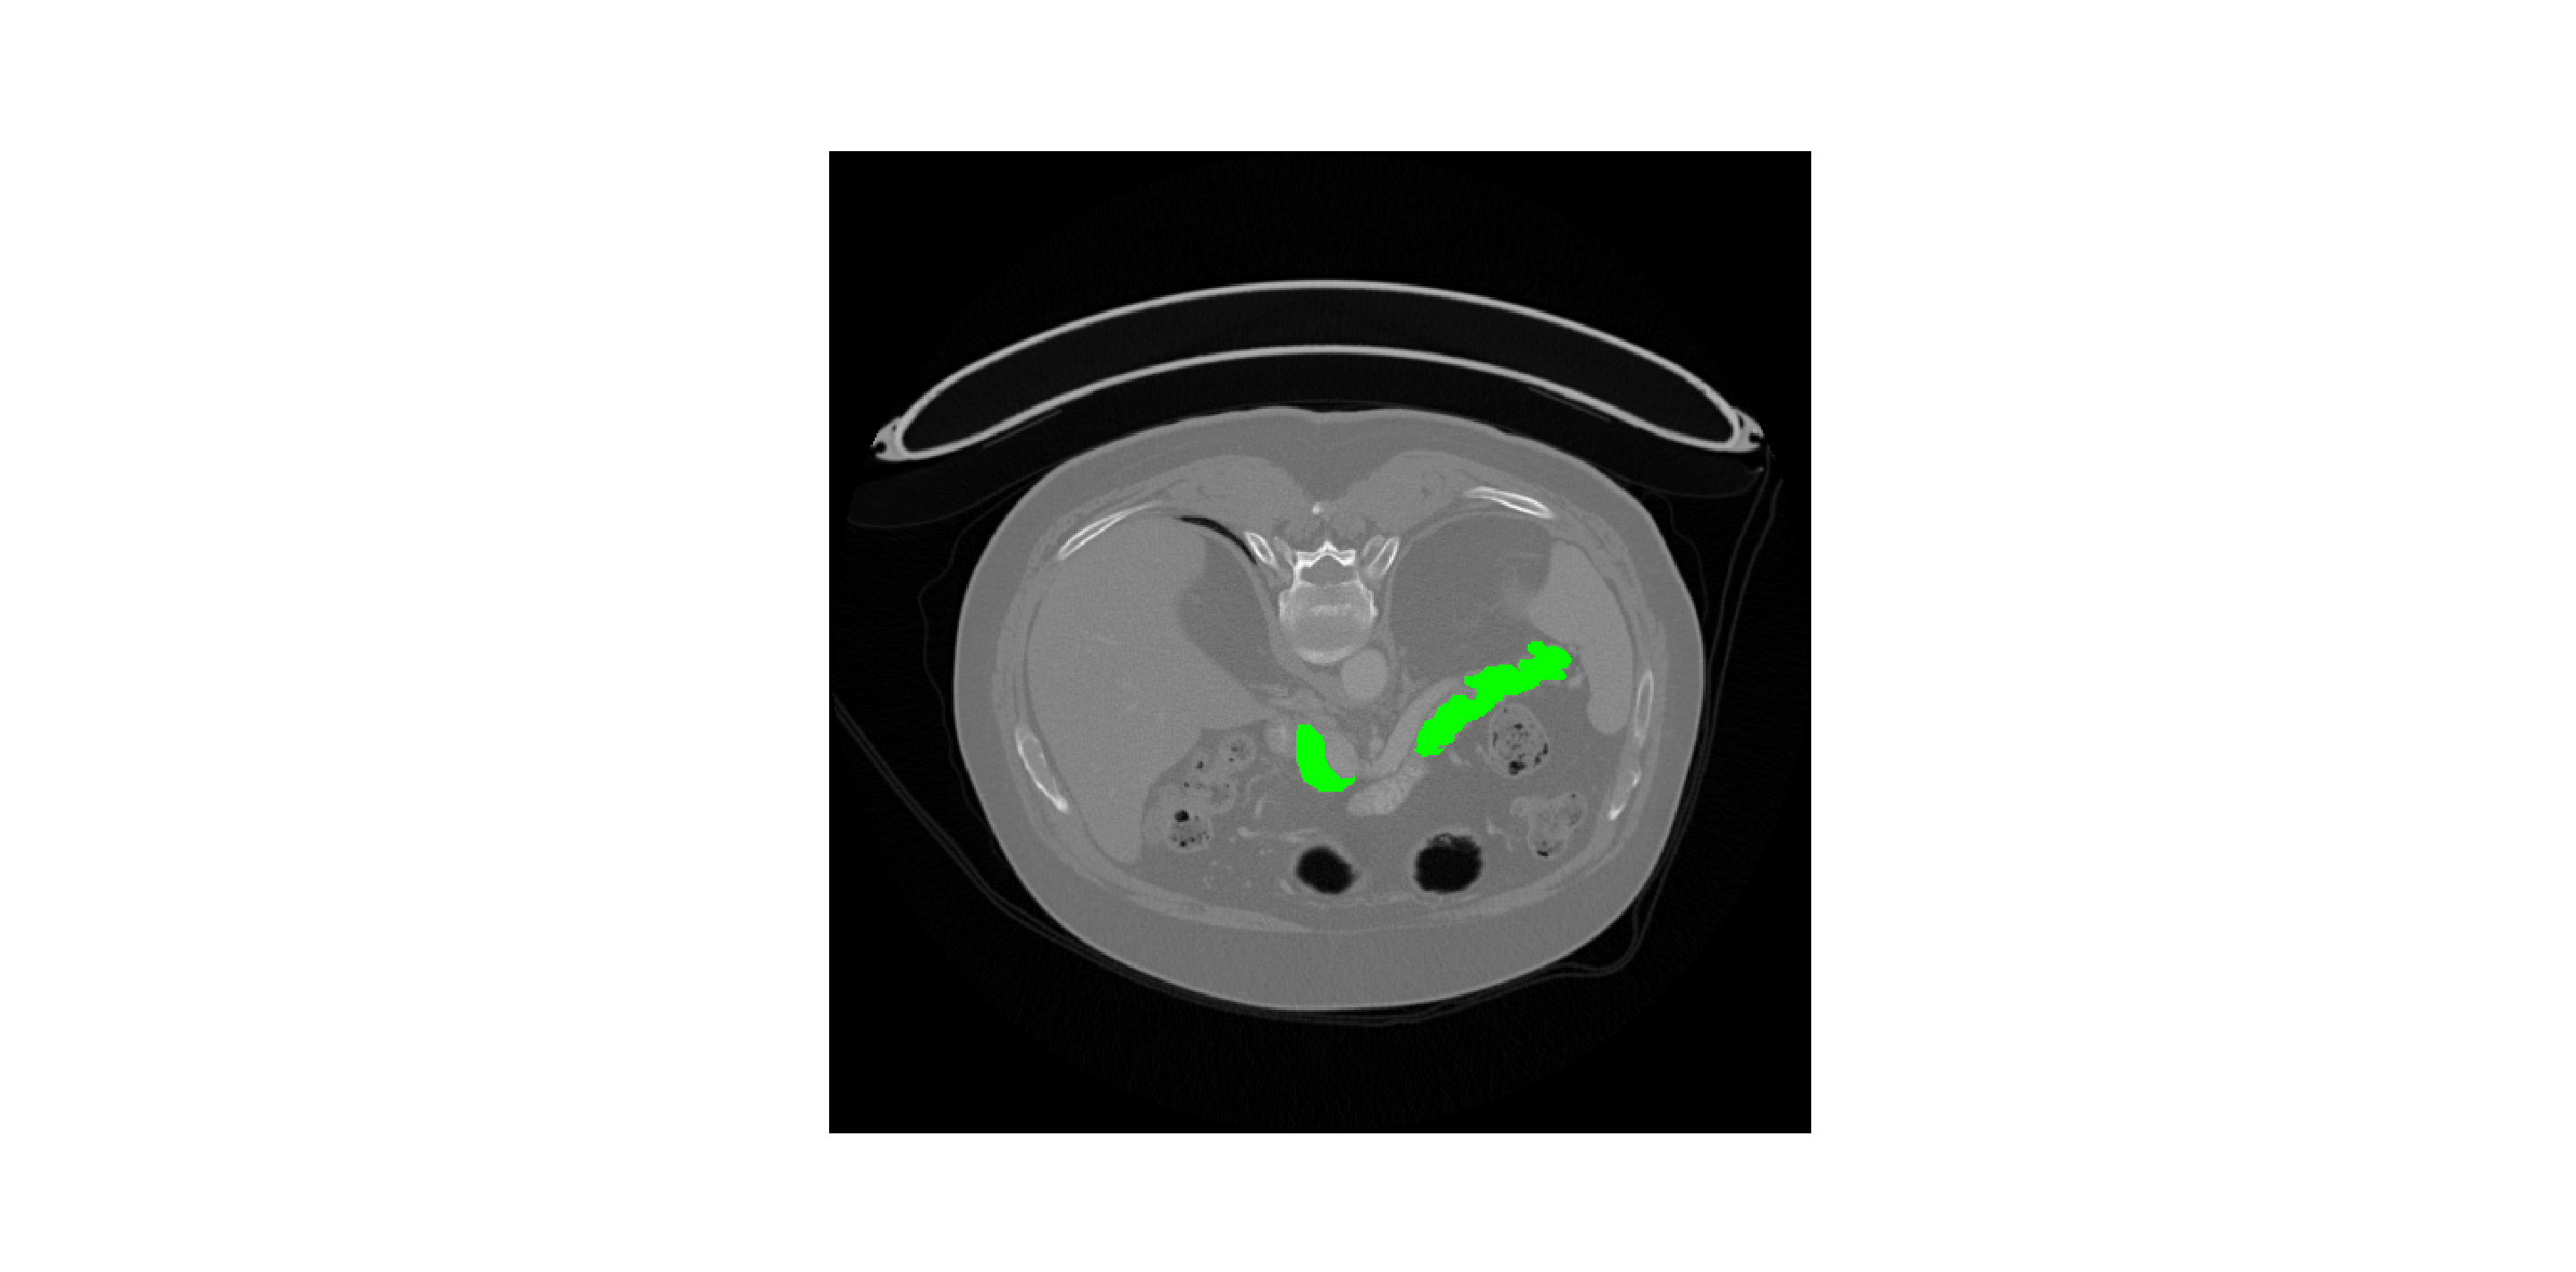
\includegraphics[scale=0.25]{Genel-Bilgiler/Figures/68gt2D.pdf} & 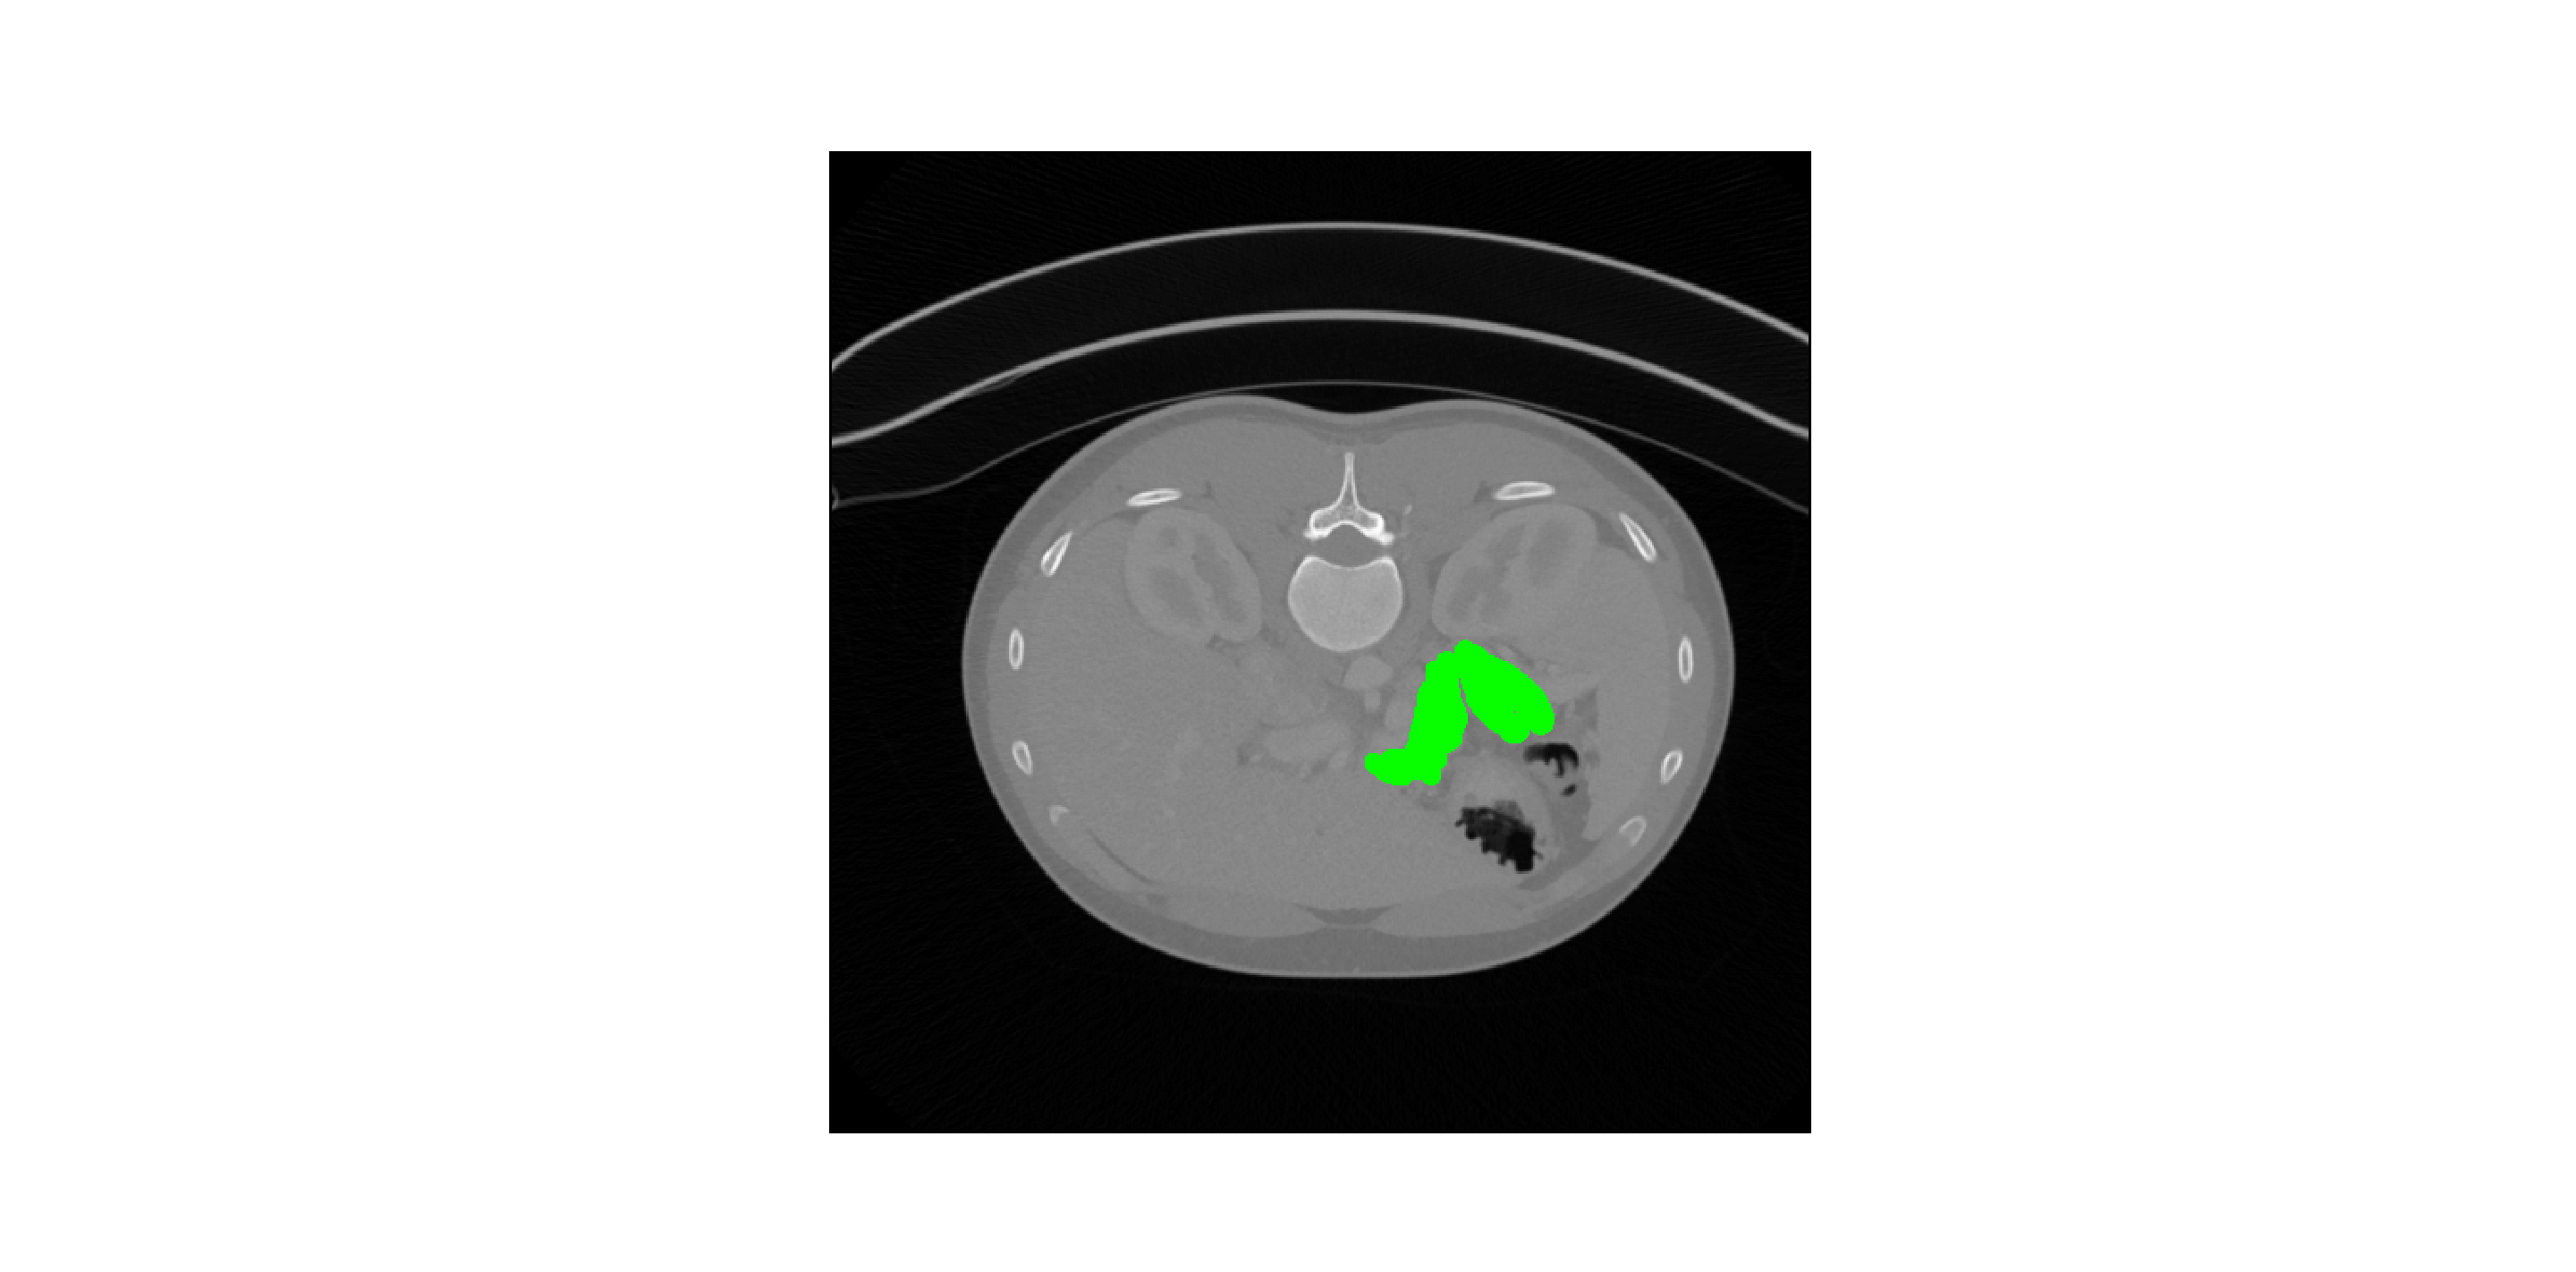
\includegraphics[scale=0.25]{Genel-Bilgiler/Figures/70gt2D.pdf} & 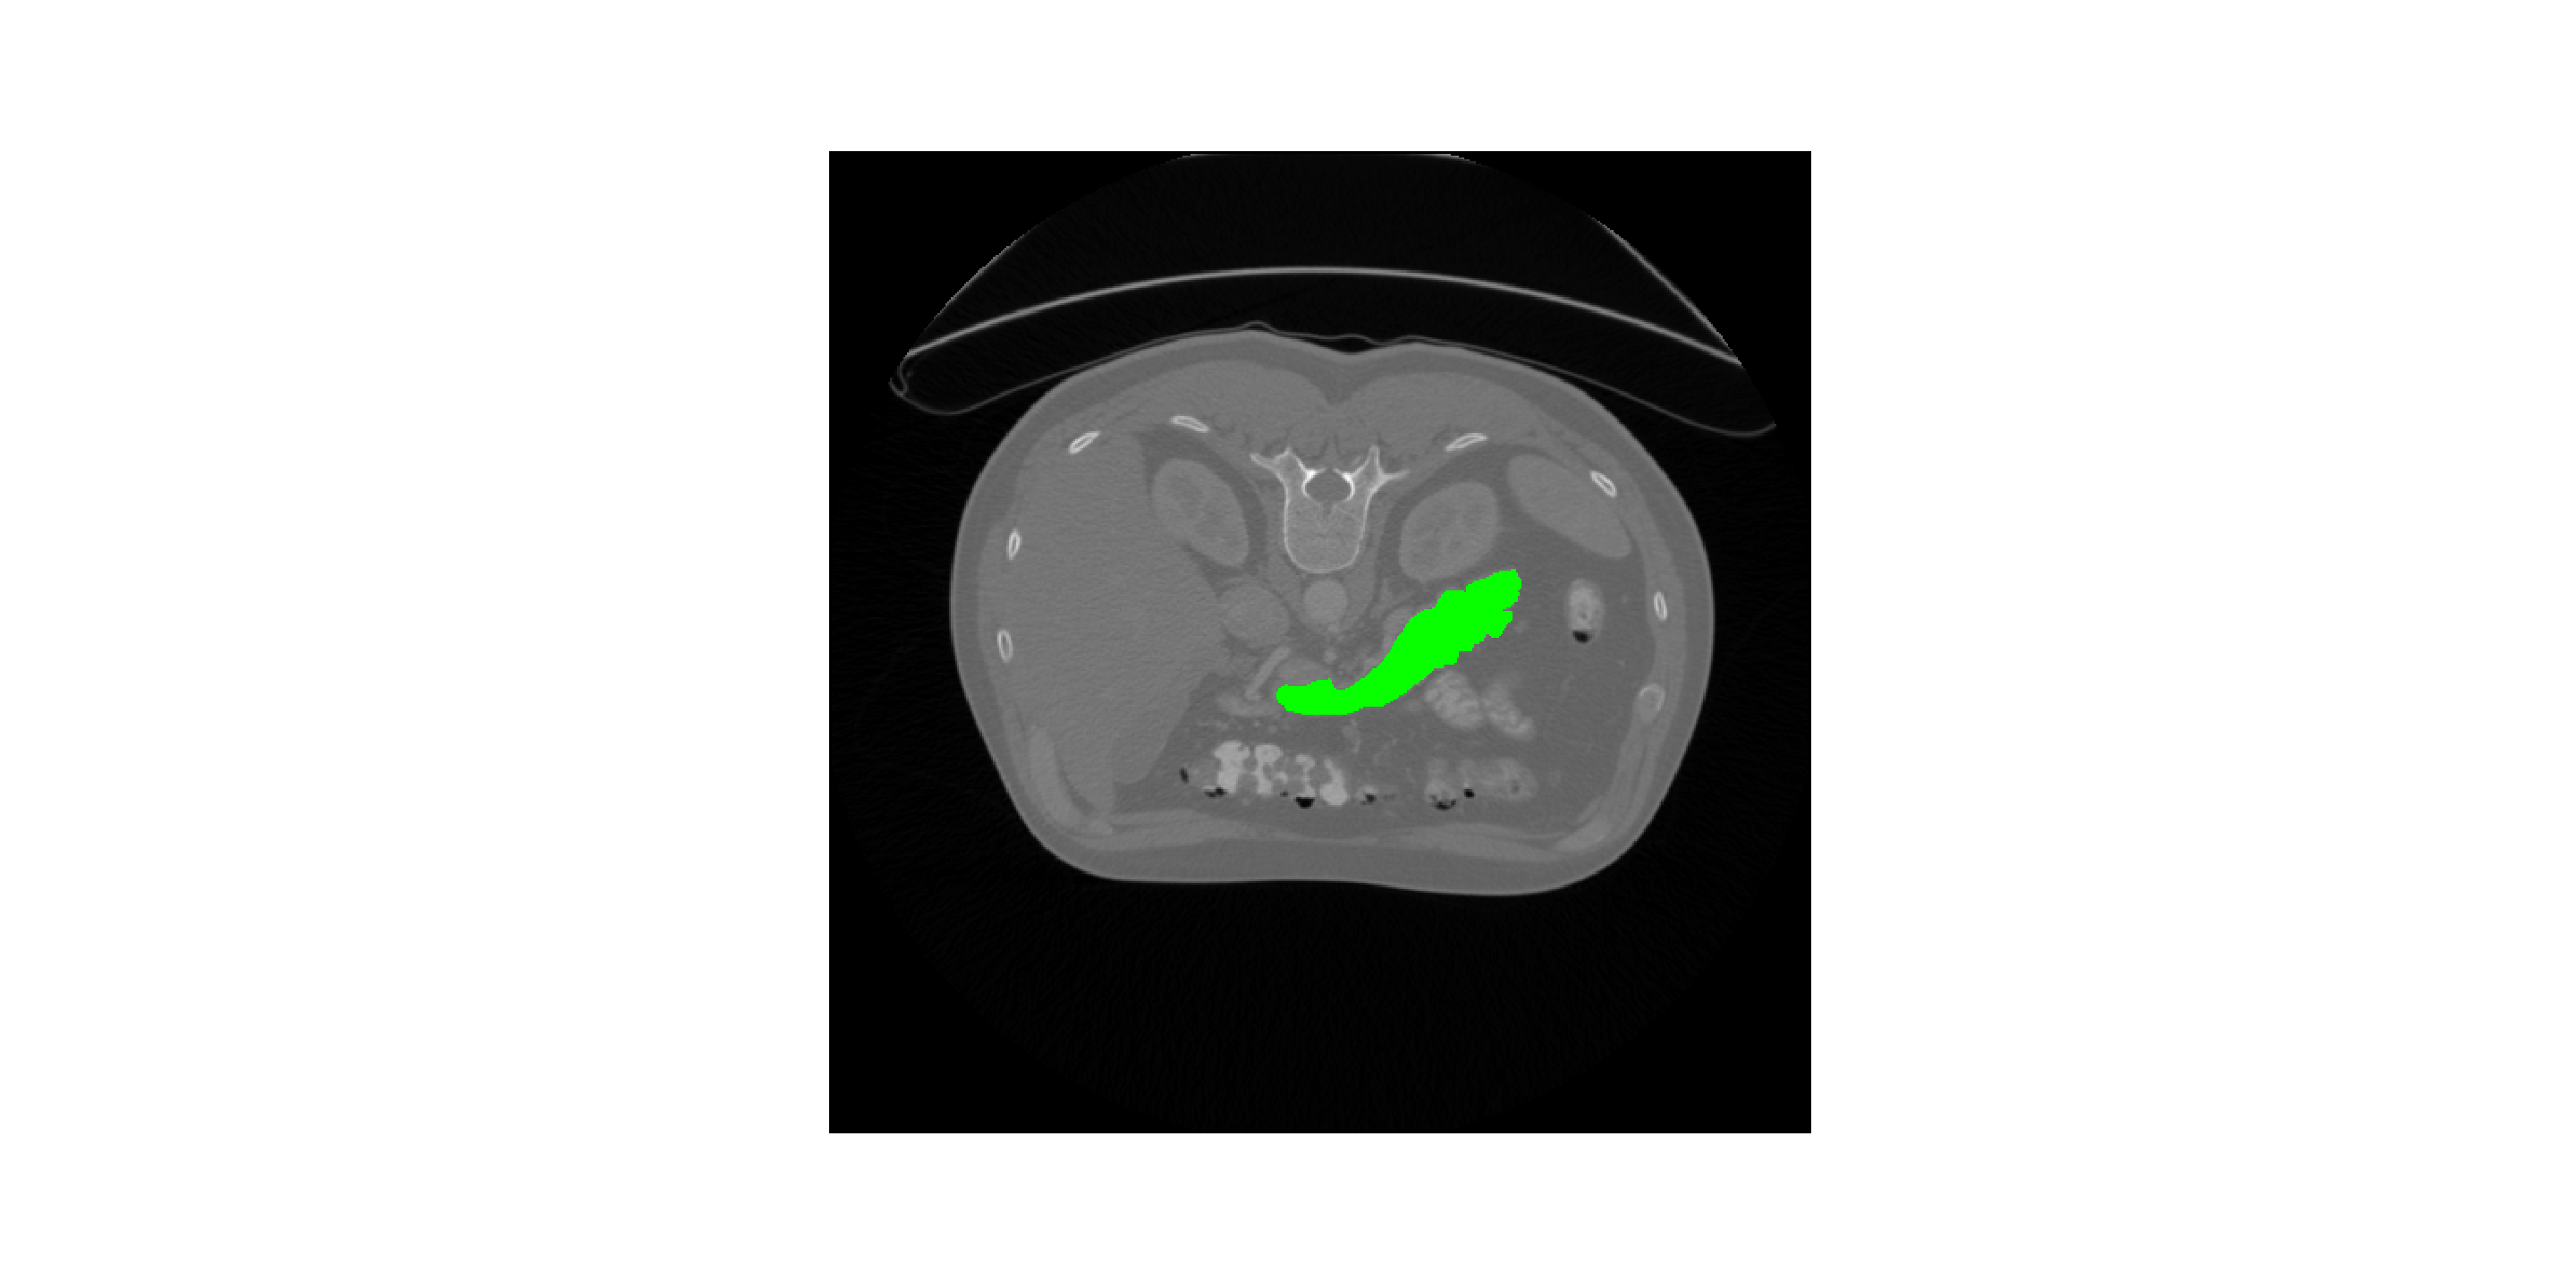
\includegraphics[scale=0.25]{Genel-Bilgiler/Figures/74gt2D.pdf} \\
				(a) &  (b)  & (c) \\
				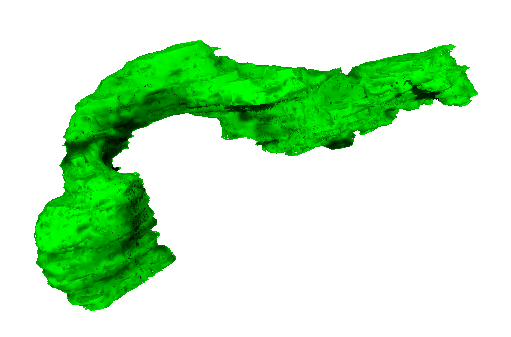
\includegraphics[scale=0.4]{Genel-Bilgiler/Figures/68gt3D.png} & 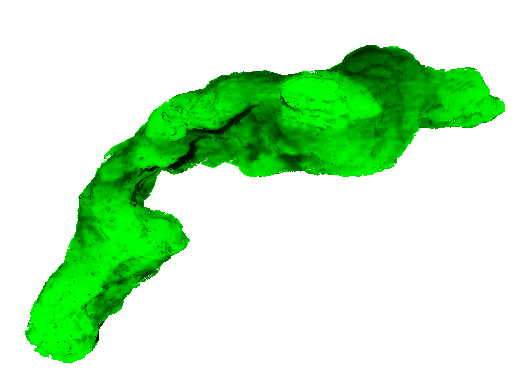
\includegraphics[scale=0.4]{Genel-Bilgiler/Figures/70gt3D.png} & 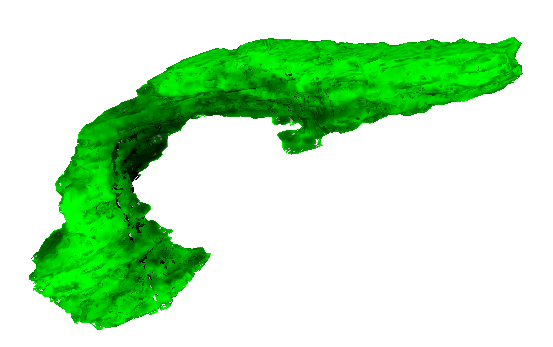
\includegraphics[scale=0.4]{Genel-Bilgiler/Figures/74gt3D.png} \\
				(d) &  (e)  & (f) 
			\end{tabular}
		}
	\end{center}
\end{figure}


Otomatik pankreas ve pankreas tümörü segmentasyonu pankreas hastalıklarına sahip kişilerin sağkalım oranını artırmak ve tanı, tedavi ve cerrahide tıp doktorlarına yardımcı olmak için kullanılmaktadır \cite{peery2019burden}. Literatür çalışmaları karaciğer, böbrek ve kalp gibi diğer abdominal organların segmentasyon başarılarının yüksek olduğunu ve tatmin edici performansların sağladığını göstermektedir \cite{peng2020method,wittenstein2019automatic,ahn2019comparative}. Oysaki Şekil \ref{fig:pancreas_types}'de görüldüğü gibi pankreasın ve pankreas tümörünün değişken büyüklükleri, şekilleri ve konumları nedeniyle, pankreas ve pankreas tümörü segmentasyonu ile ilgili çalışmalar belirli bir başarı yüzdesine kadar ulaşabilmektedirler \cite{zhao2019fully}. Tez çalışmamızın amacı literatürdeki çalışmalara göre BT görüntülemede daha yüksek doğrululuğa sahip otomatik pankreas ve pankreas tümörü segmentasyonu sağlamaktır. Bunun için bu çalışmada başarısı diğer alanlarda ispatlanmış Konvolüsyonel Sinir Ağı (Convolutional Neural Network - CNN) temelli yaklaşımlar geliştirilmektedir. Tez kapsamında gerçekleştirilen pankreas ve pankreas tümörü segmentasyonu çalışmalarının şematik temsili Şekil \ref{fig:tez_kapsami}'de gösterilmektedir. Şekil \ref{fig:tez_kapsami}'de görüldüğü gibi tez çalışması Pankreas Segmentasyonu, Pankreas ve Pankreas Tümörü Segmentasyonu olmak üzere iki ana kısımdan oluşmaktadır. 

\captionsetup[figure]{margin={0.5cm,0cm}}
\begin{figure}[h!]
	\begin{center}
		\vspace{0.4cm}
		\captionbox{Tez kapsamında gerçekleştirilen çalışmaların şematik temsili; (1) Pankreas Segmentasyonu, (2) Pankreas ve Pankreas Tümörü Segmentasyonu.
			\label{fig:tez_kapsami}}
		{
			\vspace{0.4cm}
			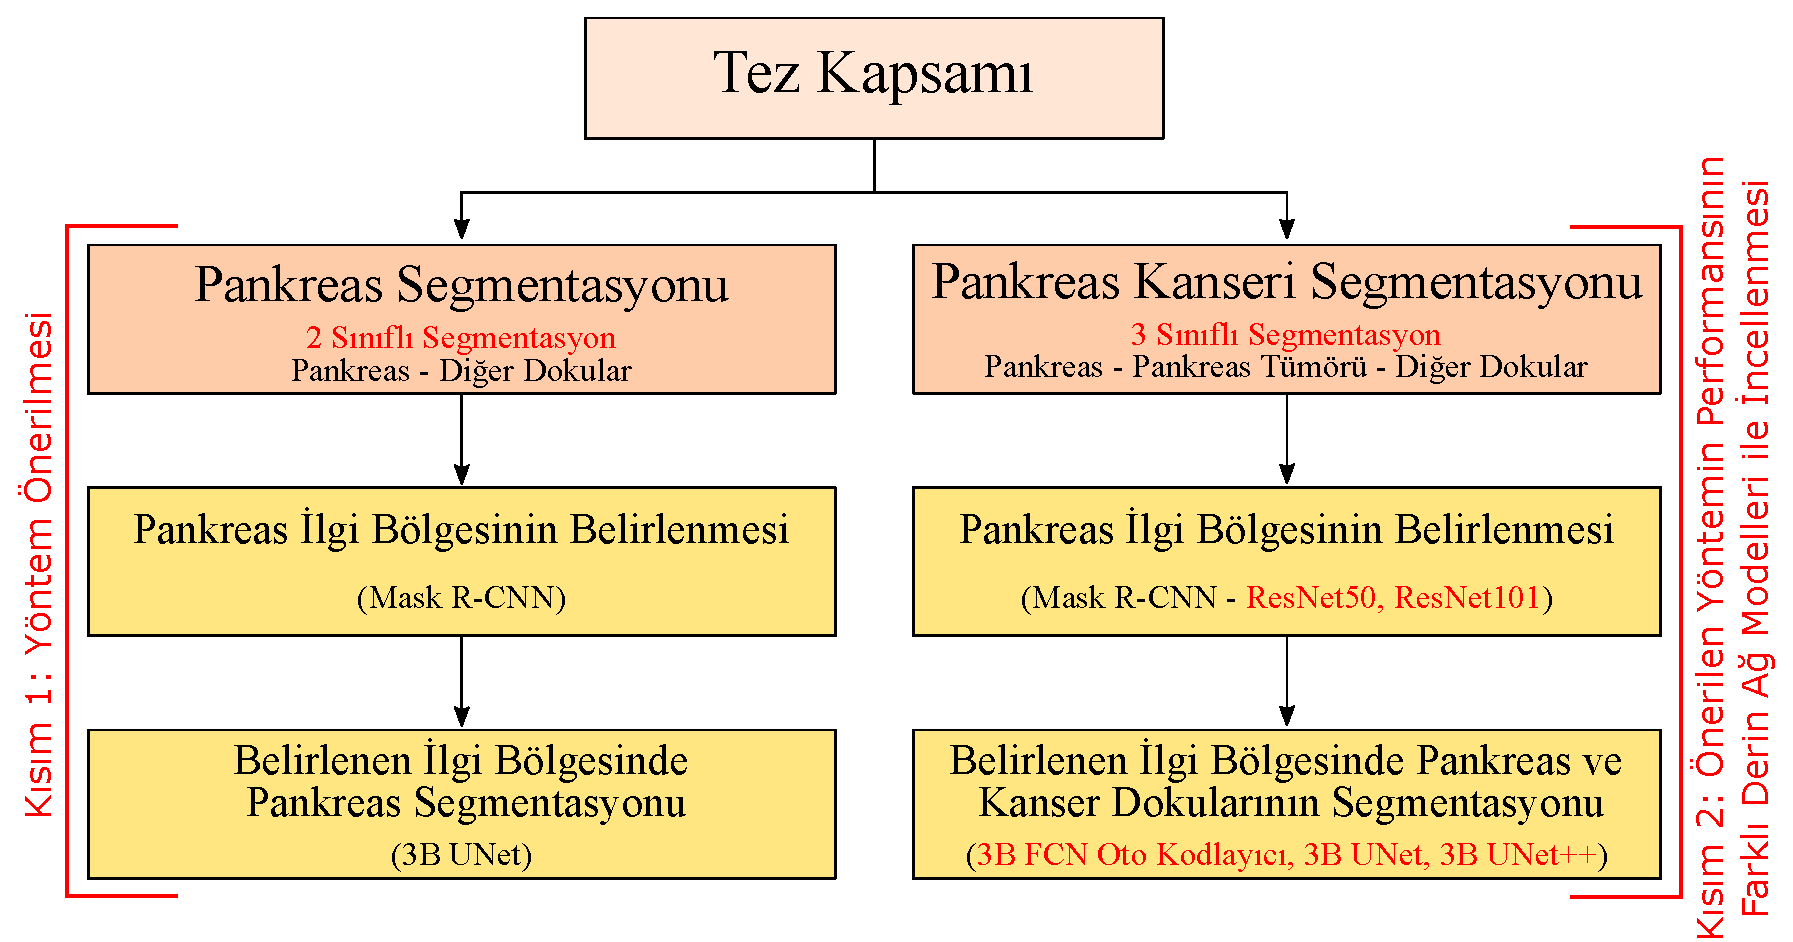
\includegraphics[scale=0.5]{Genel-Bilgiler/Figures/tezin_kapsami.pdf}
		}
	\end{center}
\end{figure}

Çalışmamızda gerçekleştirilen Pankreas Segmentasyonu kısmı Şekil \ref{fig:tez_kapsami}'de görüldüğü gibi iki ana aşamadan oluşmaktadır \cite{dogan2021two}; (i) Pankreas İlgi Bölgesinin Belirlenmesi ve (ii) Pankreas Segmentasyonu. İlk aşamada (Pankreas İlgi Bölgesinin Belirlenmesi) kaba olarak pankreas pozisyonunu tespit etmek için Maskelenmiş Bölge Esaslı Konvolüsyonel Sinir Ağı (Masked Region Proposal Convolutional Neural Network - Mask R-CNN) modeli kullanılmaktadır. Bu model tüm 2B BT dilimlerini girdi olarak almaktadır. Çıktı olarak segmente edilmiş ve maskelenmiş pankreasın aday bölgelerinin oluşturduğu 2B alt BT dilimlerini üretmektedir. İkinci aşamada (Pankreas Segmentasyonu) pankreas bölgesini daha detaylı çıkarabilmek için 3B U-Net modeli kullanılmaktadır. Bu modelde önceki aşamada üretilen 2B alt BT dilimleri girdi olarak alınmaktadır. Çıktı olarak segmente edilmiş pankreas bölgesi üretilmektedir. Pankreas segmentasyonu için önerilen yaklaşımın başarısı NIH veri setinde \cite{roth2015deep} değerlendirilmektedir. Önerilen yaklaşımın etkinliği ise performans değerlendirme metrikleri kullanılarak literatürde yüksek performans gösteren çalışmalarla karşılaştırılmaktadır. Performans değerlendirmelerinde önerilen yaklaşımın mevcut diğer yaklaşımlardan daha tatmin edici sonuçlar elde ettiği görülmektedir. 

Şekil \ref{fig:tez_kapsami}'de görüldüğü gibi tez çalışmamızın ikinci kısmı olan Pankreas ve Pankreas Tümör Segmentasyonudur. Çalışmanın Pankreas ve Pankreas Tümör Segmentasyonu kısmı da Pankreas İlgi Bölgesinin Belirlenmesi ve Pankreas ve Pankreas Tümör Segmentasyonu olmak üzere iki ana aşamadan oluşmaktadır. İlk aşamada (Pankreas İlgi Bölgesinin Belirlenmesi) kaba olarak pankreas pozisyonunu tespit etmek için Maskelenmiş Bölge Esaslı Konvolüsyonel Sinir Ağı (Masked Region Proposal Convolutional Neural Network - Mask R-CNN) modeli kullanılmaktadır. Bu model tüm 2B BT dilimlerini girdi olarak almaktadır. Çıktı olarak segmente edilmiş ve maskelenmiş pankreasın aday bölgelerinin oluşturduğu 2B alt BT dilimlerini üretmektedir. Bu modelde ResNet-50 ve Resnet-101 yapıları kullanılarak performans değerlendirmesi gerçekleştirilmektedir. İkinci aşamada (Pankreas ve Pankreas Tümör Segmentasyonu) pankreas ve pankreas tümörü bölgelerini daha detaylı çıkarabilmek için Standart Oto Kodlayıcı, 3B U-Net ve 3B U-Net++ modelleri kullanılmaktadır. Bu modellerde önceki aşamada üretilen 2B alt BT dilimleri girdi olarak alınmaktadır. Çıktı olarak segmente edilmiş pankreas ve pankreas tümör bölgeleri üretilmektedir. Pankreas ve pankreas tümör segmentasyonu için önerilen yaklaşımların başarısı Dekatlon (Medical Segmentation Decathlon - MSD) veri setinde \cite{simpson2019large} değerlendirilmektedir. Önerilen yaklaşımların etkinlikleri görmek için, çalışmamız performans değerlendirme metrikleri kullanılarak literatürde yüksek performans gösteren çalışmalarla karşılaştırılmaktadır. Performans değerlendirme metrikleri sonuçlarına göre önerilen yaklaşım mevcut diğer yaklaşımlardan daha tatmin edici segmentasyon sonuçları vermektedir. 

\subsection{Tezin Katkıları}
Tez çalışmamızın ilk kısmı olan Pankreas Segmentasyonu için önerilen yaklaşımın temel katkıları şu şekilde özetlenebilmektedir:

\begin{enumerate}
	\item Literatür çalışmaları farklı anatomik yapılara (boyut, şekil ve pozisyon) sahip pankreas gibi organların otomatik segmentasyonunun hala zorlu bir alan olduğunu göstermektedir. Bu zorluğu ortadan kaldırmak amacıyla önerilen yaklaşım bu görevi literatürdeki çalışmaların aksine, Pankreas İlgi Bölgesinin Belirlenmesi ve Pankreas Segmentasyonu olmak üzere iki ana aşamada formüle etmektedir.
	\item Daha doğru segmentasyon sonuçları üretmek, hesaplama karmaşıklığını ve maliyetini azaltmak için ilk aşamada (Pankreas İlgi Bölgesinin Belirlenmesi) obje tanıma tabanlı, gerçek zamanlı segmentasyon ve konumlandırma yapabilen Mask R-CNN modeli kullanılmaktadır.
	\item Önerilen yaklaşımın ikinci aşaması (Pankreas Segmentasyonu), önceki aşamada üretilen 2B alt BT dilimleri girdi olarak almaktadır. Bu nedenle, pankreas segmentasyonu için işlenen bölgelerin boyutu küçültülmektedir.
	\item Daha güçlü Grafik İşlemci Ünitesi (Graphics Processing Unit - GPU) kullanan literatür çalışmalarının aksine, daha düşük kapasiteli GPU kullanan tezdeki yaklaşım iki aşamadan oluşarak hem işlem belleğini azaltmakta hem de daha başarılı sonuçlar elde etmektedir.
	\item İki aşamalı yaklaşım otomatik pankreas segmentasyonu için tasarlanmış olsa da, pankreas organında görüldüğü gibi farklı yapılara sahip diğer organları segmente etmek için kolayca uyarlanabilmektedir.
	\item Önerilen yöntem pankreasın otomatik segmentasyonu için gerçek zamanlı ve tatmin edici performans sağlamaktadır.
\end{enumerate}

Tez çalışmamızın ikinci kısmı olan Pankreas ve Pankreas Tümör Segmentasyonu için önerilen yaklaşımın temel katkıları şu şekilde özetlenebilmektedir:

\begin{enumerate}
	\item Önerilen tez çalışması öncelikle Pankreas İlgi Bölgesinin Belirlenmesi aşamasında kaba pankreas bölgesini çıkarmaktadır. Daha sonra ikinci aşamada (Pankreas ve Pankreas Tümör Segmentasyonu) ilk aşamada kaba olarak bulunan pankreas bölgesinden pankreas tümör bölgesi segmente edilmektedir. Gerçekleştirilen literatür araştırmasına göre otomatik pankreas ve pankreas tümörü segmentasyonu için işlenen bölgeyi azaltarak başarıyı artıran ilk çalışmalardan biridir. 
	
	\item Otomatik pankreas tümör segmentasyonu literatürde hala zor bir alan olmasına rağmen, bu çalışmada iki aşamalı yöntem uygulanarak daha yüksek doğrulukta sonuçlar elde edilmektedir. 
	
	\item Literatür çalışmaları genellikle 2B BT görüntülerinin tüm bölgesi üzerinde otomatik pankreas tümörü segmentasyonu gerçekleştirmektedirler. Pankreas tümörlerinin farklı lokasyonları, farklı ve küçük yapıları nedeniyle tatmin edici performans sağlayamamaktadırlar. Otomatik pankreas tümörü segmentasyonu için tüm 2B BT görüntülerini işlemek yerine, önerilen yöntemimiz ilk aşamada (Pankreas İlgi Bölgesinin Belirlenmesi) kaba pankreas bölgesini tespit ederek bölgenin boyutunu küçültmektedir. 
	
	\item 2B BT görüntülerinin tüm bölgesini giriş olarak alan literatür çalışmalarından farklı olarak, bu çalışma otomatik pankreas tümörü segmentasyonu için ilk aşamada üretilen 2B alt BT görüntülerini giriş olarak almaktadır. Bu nedenle, bu çalışma daha yüksek doğruluklu pankreas tümörü segmentasyon sonuçları üretmekte, hesaplama maliyetini ve karmaşıklığını azaltmaktadır. 
	
	\item Tez çalışmasında otomatik pankreas tümörü segmentasyonu için ilk aşamada (Pankreas İlgi Bölgesinin Belirlenmesi) üretilen 2B alt BT görüntülerinin işlenmesi nedeniyle, GPU kapasitesi daha düşük olan çalışmamız, daha güçlü GPU kapasiteli diğer literatür çalışmalarına göre daha yüksek doğrulukta sonuçlar üretebilmektedir. 
	
\end{enumerate}

\chapter{YAPILAN ÇALIŞMALAR \label{sec:yapilancalismalar}}

Pankreas hastalıklarının tanı ve tedavisinde tıp doktorlarına yardımcı olmak için bu tez çalışmasında pankreas ve pankreas tümörü segmentasyonu gerçekleştirilmektedir. Bu kapsamda derin öğrenme tabanlı yaklaşımlar önerilmektedir. Tez çalışmamız iki farklı kısımdan oluşmaktadır. İlk kısımda pankreas segmentasyonunu gerçekleştirmeye yönelik iki fazlı bir yöntem önerilmektedir. İkinci kısımda ise pankreas ve pankreas tümör dokularını segmente etmek için ilk kısımda önerilen iki fazlı yöntem tekrar dizayn edilmekte ve her fazın performanslarında gerçekleştirilebilecek iyileştirmeler incelenmektedir. 

Tez çalışmasının bu bölümünde öncelikle tezde gerçekleştirilen derin öğrenme temelli yaklaşımlar için kullanılan temel derin öğrenme bilgilerine değinilmektedir. Daha sonra tezin ilk kısmı olan pankreas segmentasyonu için önerilen iki fazlı yöntem detayları ile açıklanmaktadır. Son olarak tezin ikinci fazı olan pankreas ve pankreas tümör segmentasyonu için önerilen iki fazlı yöntem farklı derin ağ modelleri ile incelenmekte ve kullanılan bu ağ modelleri detayları ile verilmektedir.

\section{Derin Öğrenmede Temel Kavramlar}
Günümüzde kullanılan modern derin öğrenme yaklaşımları temelde makine öğrenmesi yaklaşımlarının bir alt sınıfıdır. Makine öğrenmesi yaklaşımı da yapay zekanın bir alt koludur. Bu sebeple derin öğrenme, makine öğrenmesi ve yapay zeka kavramları birbiriyle direk ilişkili kronolojik sıra ile ortaya çıkmış terimler olarak görülmelidir.

Yapay zeka kavramı ilk olarak 1950'li yıllarda karşımıza çıkmaktadır. Bu alanda gerçekleştirilen ilk çalışma sinirsel aktivitelerin matematiksel yaklaşımını ortaya koymaktadır \cite{mcculloch1943logical}. Bu yıllarda yapılan başka bir çalışma ise Turing Test'tir. Bu yöntemle insan elinden çıkmış bir makinenin insan gibi düşünüp düşünemeyeceğini belirlemeye yönelik çalışılmıştır \cite{turing2009computing}. 1957 yılında yapılan bir çalışmada ilk defa Algılayıcı (Perceptron) ifadesi yer almaktadır. Ek olarak bu yıllarda ikili sınıflandırma (binary classification) yapabilen bir çalışma ortaya koyulmuştur \cite{rosenblatt1957perceptron}. 1960 yılında günümüz yapay sinir ağları ve derin çok katmanlı ileri beslemeli sinir ağları öğrenme mimarisinin temelinde yer alan Geri Yayılım Algoritması (Backpropagation) modeli ortaya atılmıştır \cite{kelley1960gradient}. Bu yöntem geliştirilerek 1962 yılında geri yayılım algoritmasında zincir kuralının yer aldığı bir çalışma gerçekleştirilmiştir \cite{dreyfus1962numerical}. 1965-1971 yılları arasında günümüz çok katmanlı sinir ağları mimarilerinin temeli niteliğinde olan çalışmalar gerçekleştirilmiştir. Bu alanda önemli ilerlemeler katedilerek Algılayıcı (Perceptron) kavramı sağlamlaştırılmıştır  \cite{ivakhnenko1971polynomial,minsky2017perceptrons}.

Makine öğrenmesi kavramı 1980'li yılların başlarından itibaren literatürde kendisine yer bulmaya başlamıştır. 1982 yılında ilk kez \textit CNN yöntemini kullanan ve el yazısı sınıflandırması yapan bir çalışma gerçekleştirilmiştir \cite{fukushima1982neocognitron}. Yine 1982 yılında Özyineli Sinir Ağları (Recurrent Neural Networks - RNN) mantığını kullanan ilk çalışma ortaya çıkarılmıştır \cite{hopfield1982neural}. 1989 yılında geri yayılım algoritması ile eğitilebilen LeNet isimli ilk CNN mimarisi gerçekleştirilmiştir \cite{lecun1989backpropagation}. 1997 yılında RNN mimarisi geliştirilerek Uzun-Kısa Vadeli Bellek (Long Short Term Memory - LSTM) mimarisi ortaya atılmıştır \cite{hochreiter1997long}. Aynı ekip tarafından 1998 yılında RNN mimarilerinde katman sayısı arttıkça ileri katmanlarda türevin çok küçüldüğü tespit edilmiştir. Bu sebeple geri yayılım algoritmasında zincir kuralıyla bu küçülen türevin ilk katmanlara etkisinin anlamsızlaştığı görülmüştür. Aynı çalışmada Kaybolan Eğim (Vanishing Gradient) adı verilen bu problem için bir çözüm önerilmiştir \cite{hochreiter1998vanishing}.

2000'li yıllarla birlikte katman sayılarının fazlasıyla artması sonucu vektörel hesaplama yeteneği yüksek olması sayesinde hesaplama maliyetini oldukça düşüren Grafik İşlemciler (Graphical Processing Unit - GPU) kullanılmaya başlanmıştır \cite{raina2009large,cirecsan2010deep,sanders2010cuda}. Yine bu yıllarda derin öğrenme algoritmalarının GPU üzerinde yüksek performans ile çalıştırılabilmesi için Torch, Theano, Tensorflow gibi kütüphaneler geliştirilmiştir \cite{collobert2002torch,bergstra2010theano,abadi2016tensorflow,paszke2019pytorch}. Ayrıca görsel nesne tanıma üzerine yarışmalar düzenlenmeye başlanmıştır. Bu amaç için 2009 yılında ImageNet isimli veri tabanı ortaya çıkarılmıştır \cite{deng2009imagenet}. ImageNet günümüzde güncellenmiş hali ile 1000 farklı sınıftan 14 milyon işaretlenmiş görüntüden oluşmaktadır. 2010-2017 yılları arasında ImageNet Büyük Ölçekli Görsel Tanıma Yarışması (ImageNet Large Scale Visual Recognition Challenge - ILSVRC) adı altında etkinlikler düzenlenmiştir. Bu yarışmalar derin öğrenme algoritmalarının gelişmesine öncülük etmiştir. 2011 yılında Doğrultulmuş Doğrusal Ünite (Rectified Linear Unit-ReLU) aktivasyon fonksiyonu kullanımının CNN mimarilerinde Kaybolan Eğim problemini ortadan kaldırabildiği görülmüştür \cite{glorot2011deep}. 2012 yılında ImageNet yarışmasında ortaya çıkan AlexNet derin öğrenme modeli sınıflandırma doğruluğunu \%75'lerden \%84'e çıkararak derin öğrenme mimarilerinin önemini ortaya koymuştur \cite{krizhevsky2012imagenet}. Derin öğrenmenin ILSVRC gibi yarışmalarda göstermiş olduğu üstün başarı bu alanda öncü Çok Derin Konvolüsyonel Ağlar (Very Deep Convolutional Networks - VGG) \cite{simonyan2014very}, Google Inception \cite{szegedy2015going}, Derin Artık Ağlar (Deep Residual  Networks - ResNet) \cite{he2016deep}, MobileNet \cite{howard2017mobilenets}, EfficientNet \cite{tan2019efficientnet} v.b.  çalışmaların ortaya çıkmalarını sağlamıştır. Yine bu yıllarda görüntü içerisinde nesnenin pozisyonunu bulmaya yönelik Bölge Tabanlı Evrişimli Sinir Ağı (Region-based Convolutional Neural Network - R-CNN) \cite{girshick2014rich}, Hızlı R-CNN (Fast R-CNN)  \cite{girshick2015fast}, Daha Hızlı R-CNN (Faster R-CNN) \cite{ren2015faster}, YOLO (You only look once) \cite{redmon2016you}, Tek Atış Dedektörü (Single-shot Detector - SSD) \cite{liu2016ssd} gibi yöntemler geliştirilmiştir. Oto kodlayıcıların ortaya çıkması ile GAN \cite{goodfellow2020generative} gibi resim çizebilen derin ağ mimarileri geliştirilmiştir. Oto kodlayıcı tekniğini kullanarak aranan nesnenin görüntü içerisinde segmentasyonuna yönelik FCN \cite{long2015fully}, U-Net \cite{ronneberger2015u} ve temelinde FCN kullanan Mask-RCNN \cite{he2017mask} gibi çalışmalar gerçekleştirilmiştir.

Günümüzde derin öğrenme ham veri girdi alarak kendi özellik haritalarını oluşturabilen ve bu özellik haritaları kullanılarak tam otomatik sınıflandırma, konumlandırma, bölütleme gibi çok farklı amaçlar için özelleştirilebilen bir yöntemdir. Geleneksel yöntemlerle çözülmesi zor problemler derin öğrenme temelli yaklaşımlarla gerçekleştirilebilmekte ve oldukca tatmin edici sonuçlar elde edilebilmektedir.

\subsection{Derin Sinir Ağları}
Derin sinir ağları (Deep Neural Network-DNN) Yapay sinir ağlarının(Artifical Neural Network-ANN) katman sayılarının artırıldığı ve eğitim aşamasında kullanılan optimizasyon tekniklerinin daha zenginleştirilerek kullanıldığı geliştirilmiş versiyonlarıdır. Çok katmanlı mimariye uygun şekilde derin sinir ağları tam bağlantılı katmanlardan oluşmaktadır. Oluşturulan bir modelde katman sayısının artması modelin daha karmaşık özellik vektörlerini öğrenebilmesini sağlamaktadır ve bir katmandaki hücre sayısının artması öğrenilebilecek sınıf sayısını artırmaktadır \cite{bengio2009learning,schmidhuber2015deep}. DNN mimarisini kullanan modellerde katman sayısının fazla olmasından dolayı ANN modellerinden farklı olarak girişinden uygulanan verilerde özellik çıkarma işlemine gerek kalmadan eğitim gerçekleştirilebilmektedir. DNN'ler tipik olarak verilerin giriş katmanından çıkış katmanına doğru geri dönmeden aktığı ileri beslemeli ağlardır. İlk başta, DNN bir sanal nöron haritası oluşturur ve aralarındaki bağlantılara (ağırlıklar) rastgele sayısal değerler atar. Ağırlıklar ve girdiler çarpılır ve 0 ile 1 arasında bir çıktı döndürür. Ağ istenen modeli doğru olarak tanımıyorsa geri yayılım algoritması ile ağırlıklar beklenen çıkışa göre belirlenen hataya göre güncellenir. Bu şekilde algoritma, verileri istenen doğrulukta işlemek için gerekli matematiksel modeli belirleyene kadar ağırlıklar güncellenmeye devam edilir.

\subsection{Konvolüsyonel Sinir Ağları}
Konvolüsyonel sinir ağları (Convolutional Neural Network - CNN) otomatik özellik çıkarmak için konvolüsyon katmanlarını kullanan derin öğrenme ağ mimarilerindendir. CNN nöronlar arasındaki bağlantı modelinin hayvan görsel korteksinin organizasyonuna benzemesi bakımından biyolojik süreçlerden esinlenerek geliştirilmiştir \cite{hubel1968receptive,fukushima1983neocognitron,matsugu2003subject}. Şekil \ref{fig:cnn}'de gösterildiği gibi özellik çıkarma ve sınıflandırma kısımlarından oluşmaktadırlar. Geri yayılım algoritması ile eğitilebilen ilk CNN modeli elle yazılan zip kodu tanıma için geliştirilmiş ve oldukça yüksek başarı ile çalıştığı görülmüştür \cite{lecun1989backpropagation}. Konvolüsyon katmanlarının güçlü özellik çıkarma yeteneği sayesinde oldukça başarılı sınıflandırma gerçekleştirebilmektedirler. Temel bir CNN mimarisi özellik haritalarını hesaplayan konvolüsyon katmanlarını takip eden havuzlama katmanlarının kaskat bağlı tekrarlarından ve bu katmanları takip eden düzleştirme katmanlarından oluşmaktadır. Düzleştirme katmanında 1B vektörlere dönüştürülen özellik haritaları tam bağlantılı katmanlara giriş olarak uygulanmakta ve sınıflandırma işlemi gerçekleştirilmektedir. 

\captionsetup[figure]{margin={0.2cm,0cm}}
\begin{figure}[h!]
	\begin{center}
		\vspace{0.4cm}
		\captionbox{CNN mimarisinde özellik çıkarma ve sınıflandırma kısımları \cite{strauch2019evolving}.\label{fig:cnn}}
		{
			\vspace{0.4cm}
			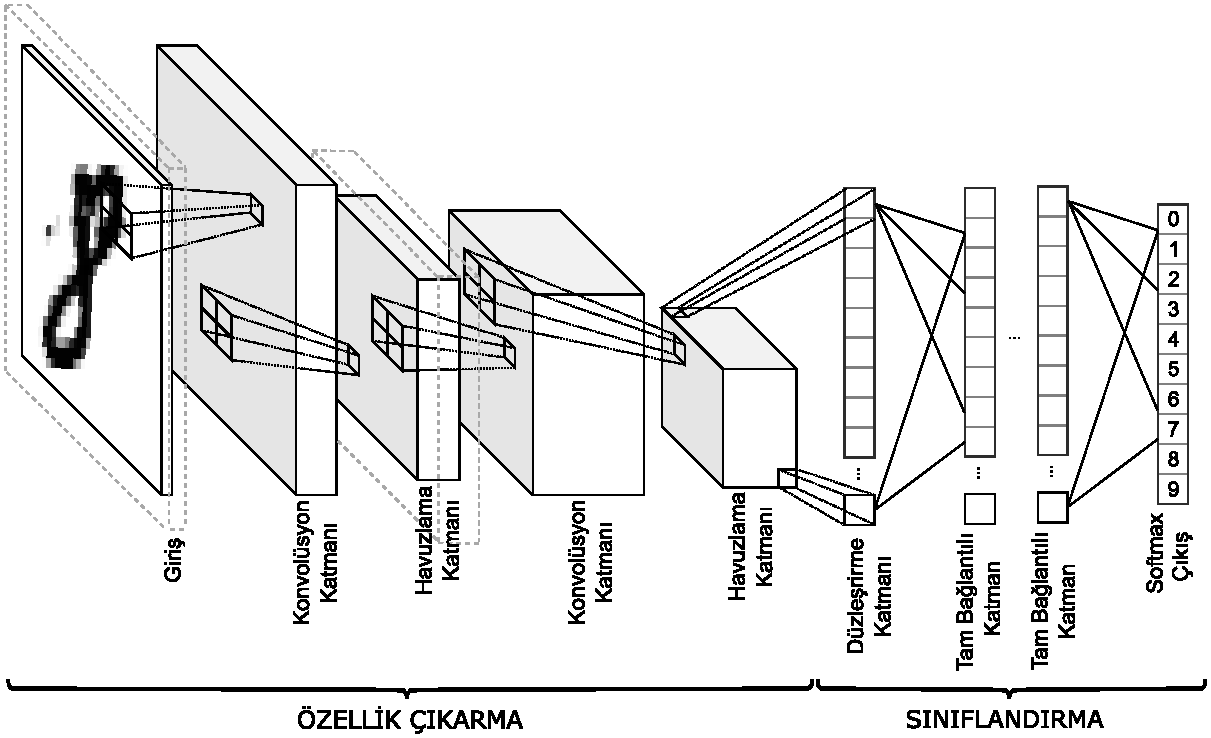
\includegraphics[scale=0.75]{Yapilan-Calismalar/Figures/cnn.pdf}
		}
	\end{center}
\end{figure}

\subsubsection{Konvolüsyonel Sinir Ağlarında Transfer Öğrenme}
Derin öğrenme sistemleri için gereken eğitim süresi ve veri miktarı geleneksel makine öğrenme sistemlerinden çok daha fazladır. Bilgisayarla görme ve doğal dil işleme gibi alanlarda geliştirilmiş ve test edilmiş, yüksek performansa sahip AlexNet \cite{krizhevsky2012imagenet}, VGG \cite{simonyan2014very}, GoogleNet \cite{szegedy2015going}, ResNet \cite{he2016deep}, MobileNet \cite{howard2017mobilenets}, EfficientNet \cite{tan2019efficientnet} gibi çeşitli derin öğrenme ağları mevcuttur. Bu modeller ImageNet \cite{deng2009imagenet} gibi oldukça fazla görüntü içeren veri tabanları ile yüksek güçlü GPU'lar kullanılarak eğitilmiş modellerdir.

\captionsetup[figure]{margin={0.2cm,0cm}}
\begin{figure}[h!]
	\begin{center}
		\vspace{0.4cm}
		\captionbox{AlexNet mimarisinden transfer öğrenme yapılarak el yazısı rakam sınıflandırma modeli.\label{fig:transfer_learning}}
		{
			\vspace{0.4cm}
			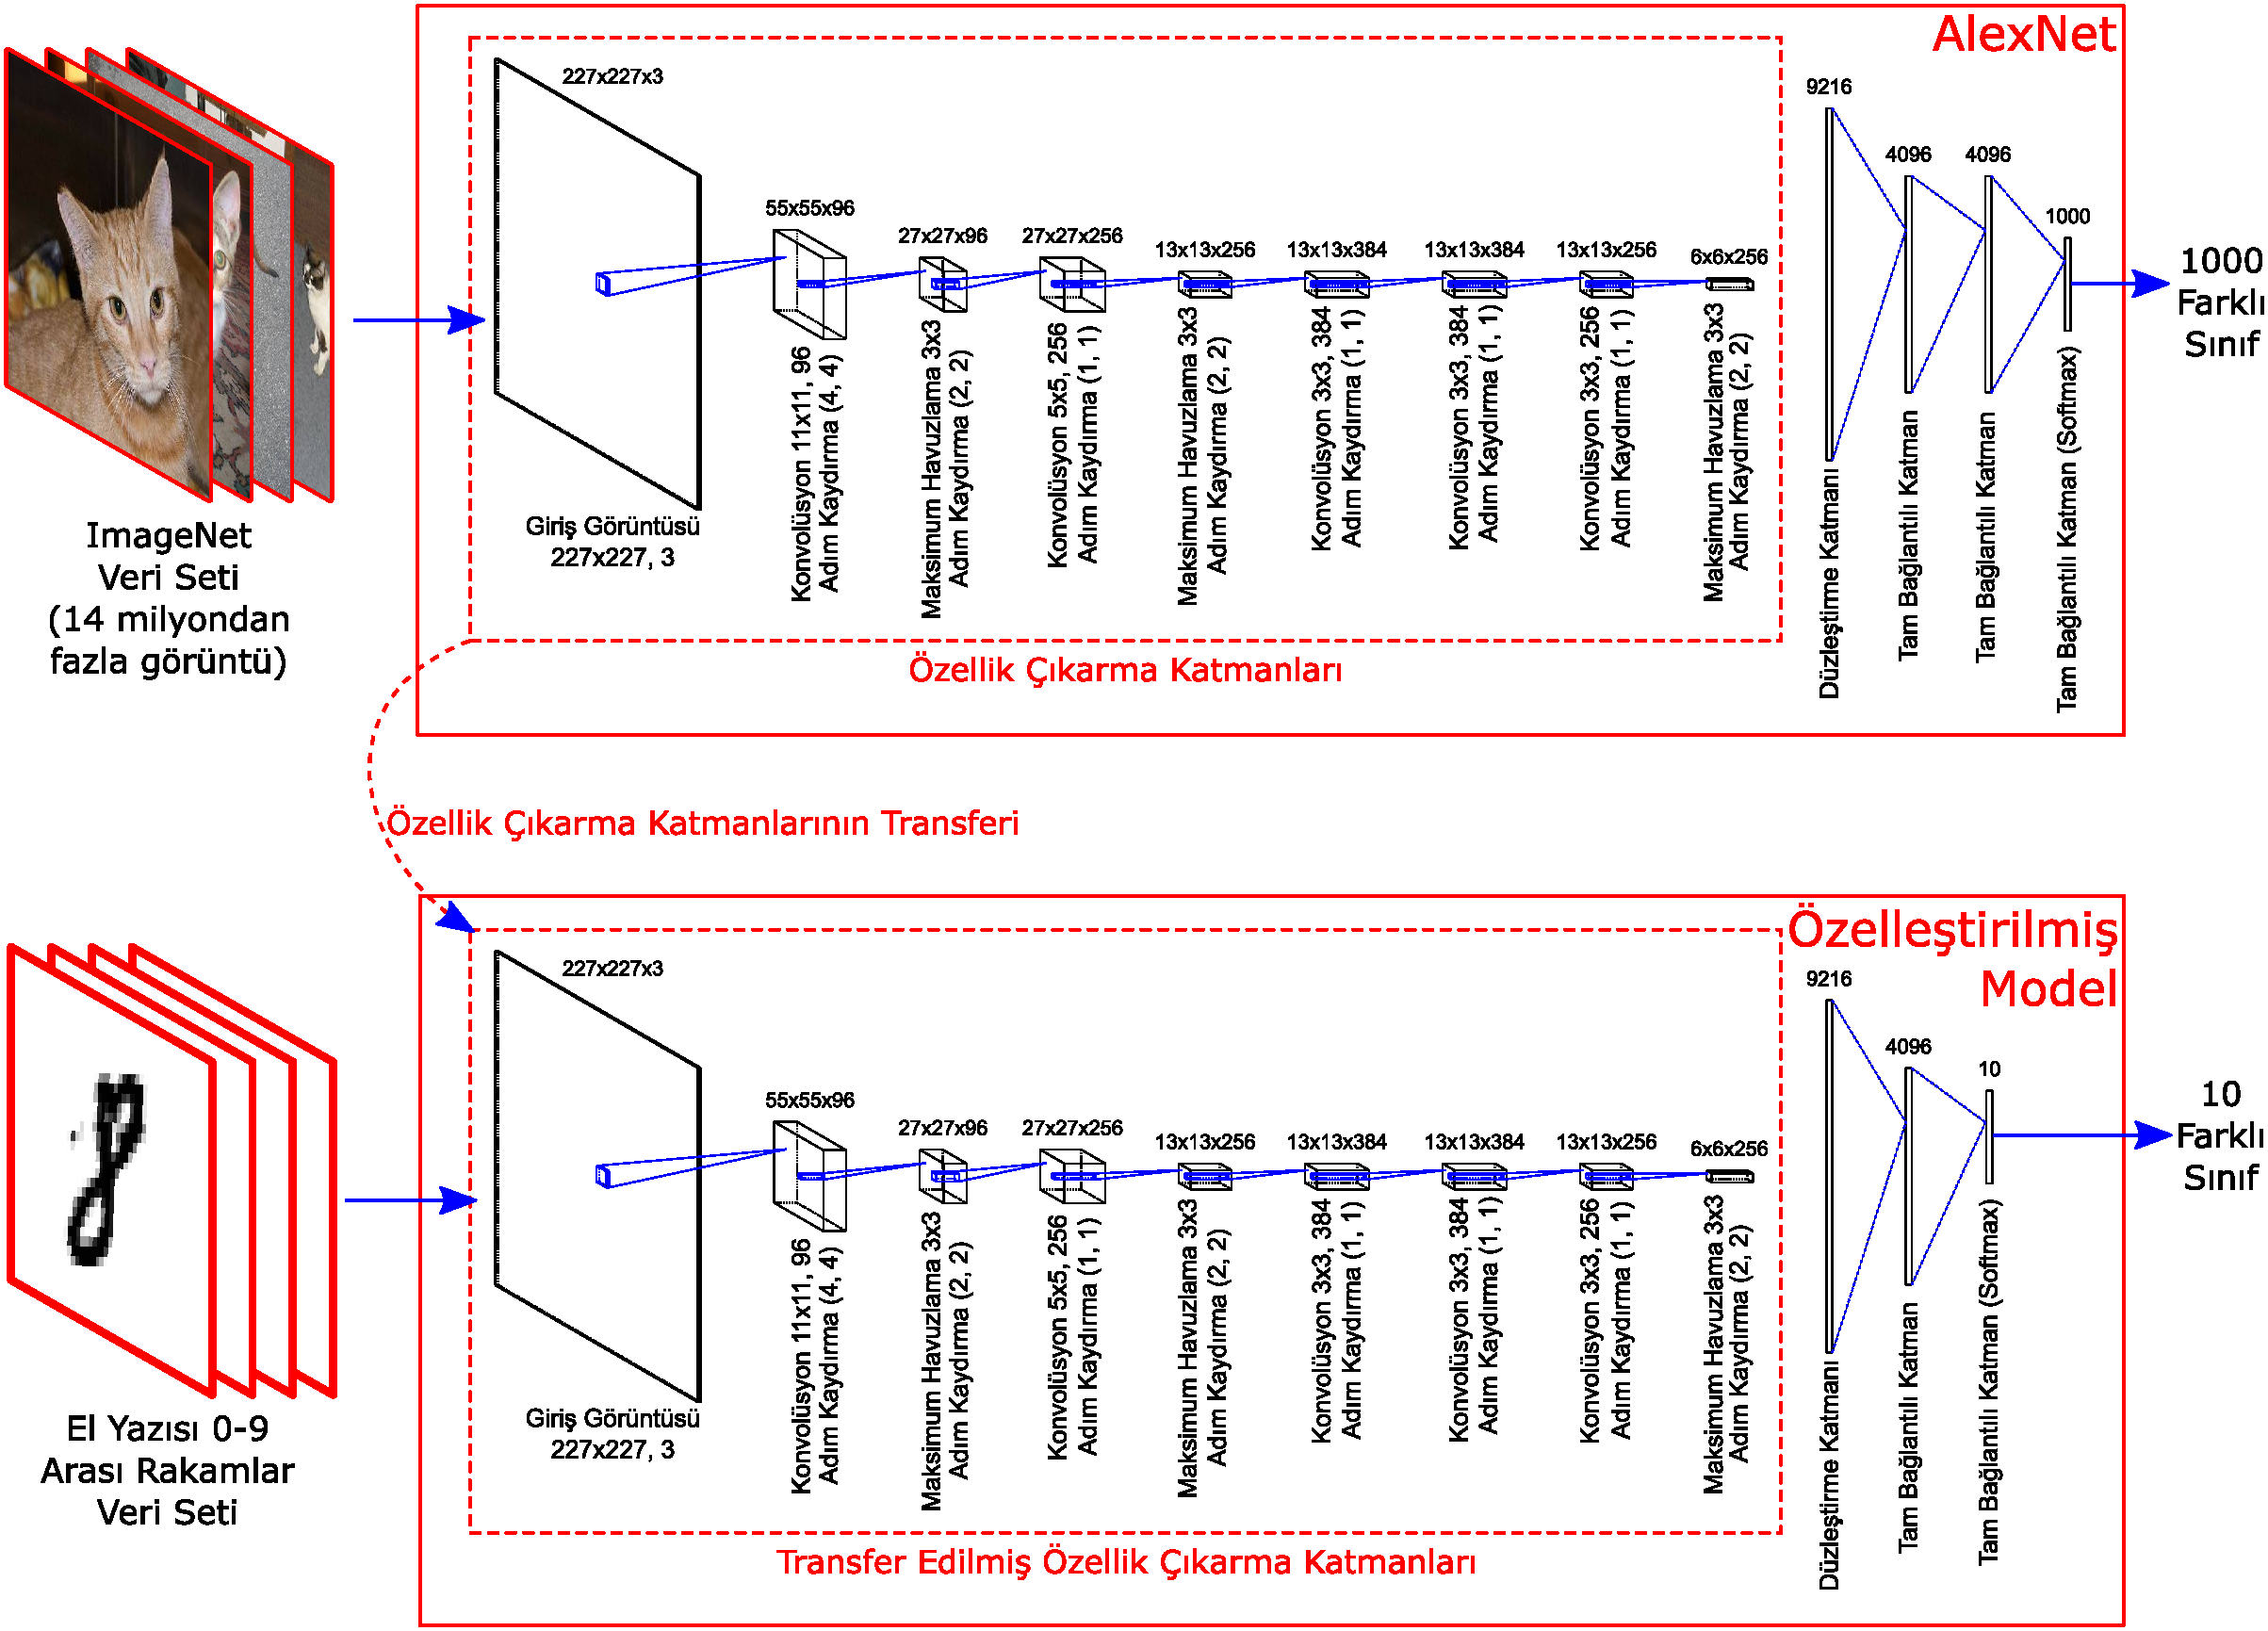
\includegraphics[scale=0.37]{Yapilan-Calismalar/Figures/transfer_learning.pdf}
		}
	\end{center}
\end{figure}

Model tabanlı transfer öğrenmedeki temel prensip daha önceden güçlü sistemler kullanılarak örnek sayısı bakımından zengin veri tabanları ile eğitilmiş yüksek performanslı modellerin özellik çıkarma katmanlarının alınarak başka sınıflandırıcı model ile birleştirilmesidir. Yeni birleştirilmiş modelde bambaşka bir veri seti kullanılarak sadece sınıflandırıcı katmanlarda eğitim gerçekleştirilmektedir. Böylece zamandan ve işlem gücünden tasarruf edilebilmektedir. Transfer edilen modelin yeni veri seti ile daha ileri seviye uyum sağlayabilmesi amaçlanmaktadır. Bu yüzden transfer edilen özellik çıkarma katmanlarının son birkaç katmanı eğitime tabi tutularak ince ayar (fine tunning) denilen eğitim gerçekleştirilmektedir. Derin özellik çıkarıcı katmanların ilk katmanları genellikle kenar doku bilgisi gibi daha genel özellik haritaları çıkarmak için özelleşirken daha derin ileri katmanları genellikle veri setine özgü özelliklerin öğrenilmesinde uzmanlaşmaktadır. Bu sebeple ince ayar ile birlikte veri setine özgü özelliklerin öğrenildiği özellik çıkarıcı katmanlar eğitime tabi tutulmakta ve veri setinin daha uygun özellik haritalarının elde edilmesi sağlanmaktadır.

Örneğin Şekil \ref{fig:transfer_learning}'de ImageNet veri tabanında eğitilmiş AlexNet mimarisi görülmektedir. Imagenet veri seti toplamda 14 milyondan fazla görüntüye sahip 1000 farklı sınıftan oluşmaktadır. ImageNet veri setinde eğitimi gerçekleştirilmiş AlexNet modelinin eğitilmiş özellik çıkarma katmanları Şekil \ref{fig:transfer_learning}'de gösterildiği gibi alınmıştır. 0 - 9 arasında el yazısı görüntülerinden oluşan bambaşka bir veri setine uygun sınıflandırma katmanları eklenmiştir. Bu modelde sadece sınıflandırma katmanlarının eğitimi gerçekleştirilebilmektedir. Bu eğitimde daha özel özellik haritaları üretebilmek için transfer öğrenme ile gelmiş özellik çıkarma katmanları istenen sayıda dahil edilerek eğitim gerçekleştirilebilmektedir. 

\subsection{Oto Kodlayıcılar}
Oto kodlayıcılar (Auto - encoders) girişinden verilen veriyi işleyerek çıkışından yine girişinden uygulanan veri ile aynı boyutlarda veri üreten derin ağlardır. Gürültü azaltma, veri sıkıştırma, veri bölütleme gibi çeşitli alanlarda kullanılmaktadır. Bu tez çalışmasında oto kodlayıcılar görüntü bölütleme amacıyla kullanılmıştır.

\captionsetup[figure]{margin={0.3cm,0.2cm}}
\begin{figure}[h!]
	\begin{center}
		\vspace{0.4cm}
		\captionbox{Oto-kodlayıcı kodlama ve kod çözme katmanları.\label{fig:autoencoder}}
		{
			\vspace{0.4cm}
			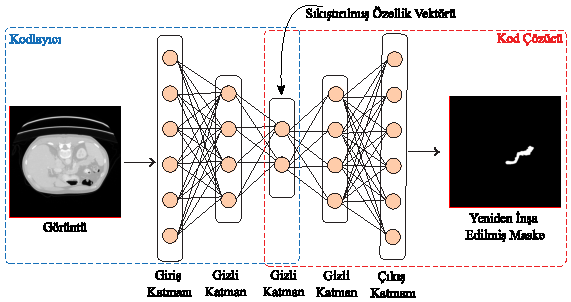
\includegraphics[scale=1.6]{Yapilan-Calismalar/Figures/autoencoder.pdf}
		}
	\end{center}
\end{figure}

Oto kodlayıcılar Şekil \ref{fig:autoencoder}'te gösterildiği gibi kodlama ve kod çözme katmanlarından oluşmaktadır. Oto kodlayıcılarla görüntü bölütleme gerçekleştirirken giriş görüntüsüne $x$, çıkışta inşa edilecek maske görüntüsü $r$, giriş $x$ görüntüsünün $f$ fonksiyonu ile kodlaması sonucu üretilecek sıkıştırılmış özellik vektörü $h$ ve sıkıştırılmış özellik vektöründen $r$ çıkış görüntüsünü elde etmek için gerekli kod çözücü fonksiyon $g$ olmak üzere, oto kodlayıcı kodlama denklemi Eşitlik \ref{eq:encode}, kod çözme denklemi ise Eşitlik \ref{eq:decode} ile temsil edilmektedir. Oto kodlayıcılarda öğrenilen bilgi $f(x)$ ve $g(h)$ fonksiyonları olmaktadır.
\begin{equation}
	\label{eq:encode}
	f(x)=h
\end{equation}
\vspace{-1.5cm}
\begin{equation}
	\label{eq:decode}
	g(h)=r
\end{equation}

\subsection{Derin Ağlarda Kullanılan Katmanlar}
Derin öğrenme çok fazla sayıda farklı türlerdeki katmanları birleştirerek çalıştırmayı gerektirmektedir. Örneğin ham veriden, veriye özgü özellik çıkarımı için konvolüsyon (evrişim) katmanları kullanılmaktadır. Ayrıca bu çıkarılan özelliklerin doğrusal olmamasını sağlayabilmek için doğrusal olmayan aktivasyon fonksiyonlarının kullanıldığı aktivasyon katmanları kullanılmaktadır. Konvolüsyon katmanlarından sonra ortaya çıkan yeni büyük ölçekli özellik haritalarının hesaplama maliyetinin azaltılması için mevcut verinin tekrar ölçeklenebilmesini sağlayan havuzlama katmanları kullanılmaktadır. Ayrıca sınıflandırma problemlerinde özellik çıkarma katmanlarından elde edilen özellik haritalarından sınıf tahmini yapabilen sınıflandırma katmanları bulunmaktadır. Derin öğrenme modelleri bunların dışında birçok farklı eğitilebilir ya da eğitilemeyen katmanlardan oluşabilmektedirler. Katmanlar birbirleri ile bir zincirin halkaları gibi bağlı olduğu için modelin eğitiminde genellikle gradyan öğrenme teknikleri tercih edilmektedir. Eğitilebilir bütün katmanlarda bir sonraki katmandan gelen türev bilgisi kullanılarak eğitim optimizasyonu gerçekleştirilmektedir. Eğitilemeyen havuzlama, düzleştirme gibi katmanlar eğitim aşamasında sadece türevin bir önceki katmana taşınmasını sağlamaktadırlar.

%\iffalse
%\begin{table}[h!]
%	\begin{tabular}{lll}
%		Konvolüsyon Katmanı      & Conv1D, Conv2D, Conv3D                            &  \\
%		Ters Konvolüsyon Katmanı & Conv1DTranspose, Conv2DTranspose, Conv3DTranspose &  \\
%		Sık Örnekleme Katmanı    & UpSampling1D, UpSampling2D, UpSampling3D          &  \\
%		Aktivasyon Katmanları    & Sigmoid,Tanh, ReLU,PReLU,ELU                      &  \\
%		Normalizasyon Katmanları & Normalization, BatchNormalization          &  \\
%		Birleştirme Katmanları   & Add, Concatenate          &  \\
%		Havuzlama Katmanları   & Add, Concatenate          &  \\
%	\end{tabular}
%\end{table} 
%\fi

\subsubsection{Tam Bağlantılı Katmanlar}
Tam Bağlantılı (Fully Connected - FC) katmanlar aslında derin öğrenme mimarilerinin sınıflandırıcı katmanlarını temsil etmektedir. Yoğun (Dense) katman olarak da adlandırılmaktadırlar. Temelde derin öğrenme çalışmaları için İleri Beslemeli Sinir Ağları (Feed Forward Neural Network - FNN) mimarilerinden biri olan Çok Katmanlı Algılayıcılar (Multi Layer Perceptron - MLP) mimarisi tercih edilmekte ve derin öğrenmeyi anlayabilmek için MLP mimarisinin matematiksel modelini anlamak gerekmektedir.

\captionsetup[figure]{margin={0.4cm,-3cm}}
\begin{figure}[h!]
	\begin{center}
		\vspace{0.4cm}
		\captionbox{MLP mimarisinin temelini oluşturan algılayıcı blok diyagramı\label{fig:perceptron}}
		{
			\vspace{0.4cm}
			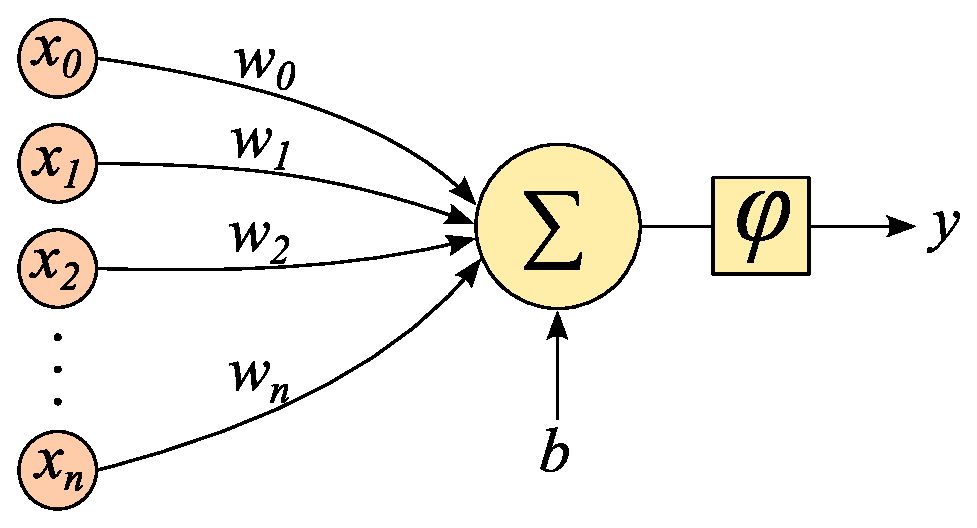
\includegraphics[scale=0.55]{Yapilan-Calismalar/Figures/perceptron.pdf}
		}
	\end{center}
\end{figure}

İlk Algılayıcı (Perceptron) matematiksel modeli 1958 yılında ortaya atılmıştır \cite{rosenblatt1957perceptron}. Başlangıçta hiperdüzlem üzerindeki doğrusal problemin çözümüne yönelik geliştirilen algılayıcılar, doğrusal olmayan aktivasyon fonksiyonlarını kullanan MLP mimarisine geçilerek hiper düzlem üzerinde doğrusal dağılmamış verilerin sınıflandırılması içinde kullanılabilir hale getirilmiştir. Algılayıcılar insan sinir hücresinin basit bir modelli gibi çalışmaktadır. Algılayıcı modeli girişinden $x_{0}, x_{1},..., x_{n}$ şeklinde  $n$ adet elemana sahip bir vektör almaktadır. Giriş vektörünün her bir elemanı kendisine karşılık gelen $w_{0}, w_{1},..., w_{n}$ ağırlıkları ile çarpılarak ana düğümde toplanmaktadır. Bu yaklaşımda girişten gelen $x$ değerlerinin hepsinin sıfır olması durumunda $w$ ağırlık değerlerinin anlamsızlaşabileceği için genel toplama bir yanlılık (bias - $b$) değeri eklenmektedir. Genel toplam doğrusal olmayan ve öğrenme aşamasında kullanım kolaylığı sağlaması amacıyla türevi hesaplanabilir bir aktivasyondan ($\varphi$ ) geçirilmekte ve Şekil \ref{fig:perceptron}'te gösterildiği gibi bir $y$ çıkışı elde edilmektedir. 

Algılayıcının girişinden uygulanan $x$ değerleri ile $y$ çıkışının hesaplanması Eşitlik \ref{eq:perceptron}'te verildiği gibi gerçekleştirilmektedir.
\begin{equation}
	\label{eq:perceptron}
	y = \varphi(\sum_{i}w_{i}x_{i} + b)
\end{equation}

\captionsetup[figure]{margin={0.4cm,-3cm}}
\begin{figure}[h!]
	\begin{center}
		\vspace{0.2cm}
		\captionbox{Tam bağlantılı katmanın blok diyagramı\label{fig:ithlayer}}
		{
			\vspace{0.2cm}
			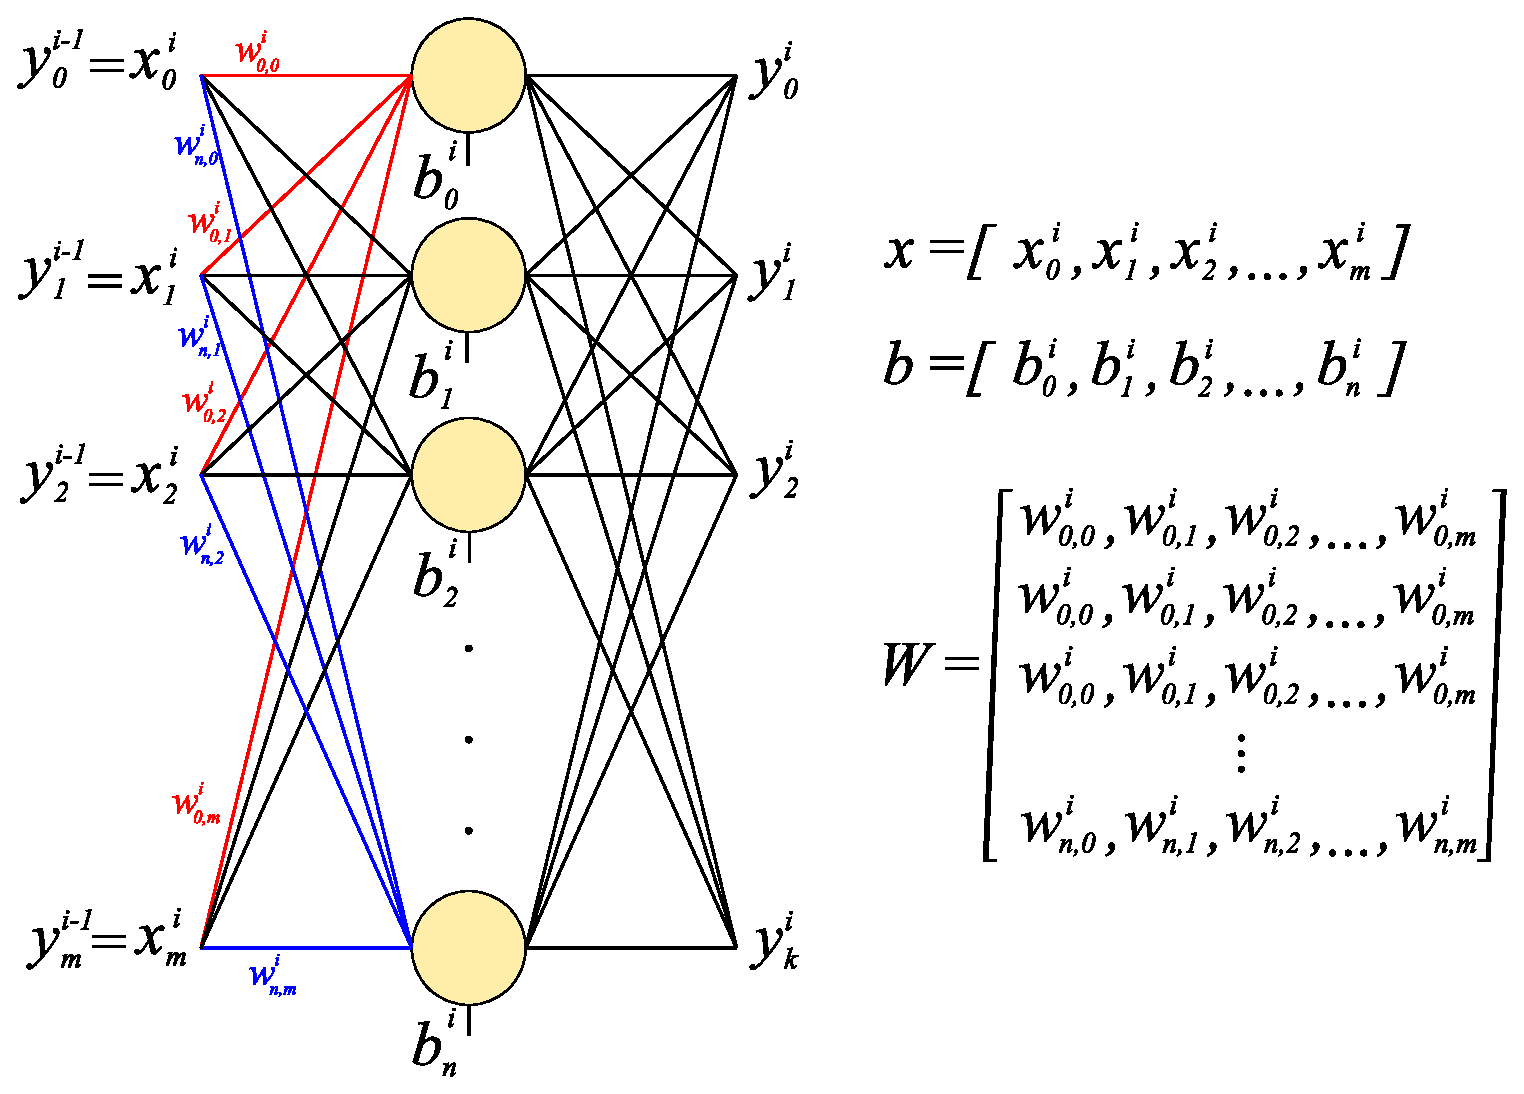
\includegraphics[scale=0.55]{Yapilan-Calismalar/Figures/ithlayer.pdf}
		}
	\end{center}
\end{figure}

Çok katmanlı ve her bir katmanında farklı sayılarda algılayıcılardan oluşan bir mimari düşünüldüğünde herbir algılayıcı çıkışının ayrı ayrı hesaplanması gerekmektedir. Bu tip yapılarda $m$ bir önceki $i-1$ inci katmandan gelen giriş değerlerinin adetini göstermek üzere $i$ inci katmandaki $x$ giriş ifadelerini $\overset{\rightarrow}{x} = \left[ x_{0}^{i}, x_{1}^{i}, x_{2}^{i},..., x_{m}^{i} \right]$ şeklinde bir vektör olarak düşünürsek. Yine ilgili $i$ inci katmandaki $n$ adet algılayıcının yanlılık $b$ değerlerini de $\overset{\rightarrow}{b} = \left[ b_{0}^{i}, b_{1}^{i}, b_{2}^{i},..., b_{n}^{i} \right]$ şeklinde bir vektör olarak düşünmek gerekmektedir. Bu doğrultuda $i-1$ inci katmandan gelen her bir girişin tam bağlantılı olarak $i$ inci katmandaki algılayıcılara giden ağırlıkları Şekil \ref{fig:ithlayer}'te gösterildiği gibi $W$ şeklinde bir matris ile temsil etmek gerekmektedir.  

Çok algılayıcılı katman mimarisi için gerekli vektör, matris dönüşümleri gerçekleştirildikten sonra tam bağlantılı katmanın ileri yönde hesaplaması Eşitlik \ref{eq:fclayer}'teki gibi gerçekleştirilerek $\overset{\rightarrow}{y}$ çıkış vektörü hesaplanabilmektedir. 
\begin{equation}
	\label{eq:fclayer}
	y = \varphi(Wx + b)
\end{equation} 

Eşitlik \ref{eq:fclayer}'te $\varphi$ aktivasyon fonksiyonunu temsil etmektedir. Varsayılan aktivasyon fonksiyonu $f(x) = x$ şeklindeki Doğrusal Aktivasyon fonksiyonudur. Bu katmanda aktivasyon fonksiyonu belirtilebileceği gibi tamamen farklı bir katmanmış gibi bu katmanın ardından aktivasyon katmanı eklenerek de kurulacak çok katmanlı mimarinin doğrusal olmayan çıkışlar üretmesi sağlanabilmektedir.

Tam bağlantılı katman ardından yine bir katman eklenebileceği gibi direk çıkış katmanı olarak da kullanılabilmektedir. Tam bağlantılı katman çıkış katmanı olarak kullanıldığında bu katmanda kullanılan aktivasyon fonksiyonu modelin eğitiminde kullanılacak optimizasyon tekniğini de belirleyen etken olarak karşımıza çıkmaktadır. Aynı zamanda verinin eğitim etiketlerinin hangi aralıkta olması gerektiğini de belirleyen faktör aktivasyon fonksiyonunun karakteristiğidir. 

\captionsetup[figure]{margin={0.3cm,-2.5cm}}
\begin{figure}[h!]
	\begin{center}
		\vspace{0.4cm}
		\captionbox{Tam bağlantılı katmanda bir sonraki katmandan gelen hata bilgisine göre zincir kuralı kullanılarak kısmi türevlerin hesaplanması\label{fig:perceptronDerivative}}
		{
			\vspace{0.4cm}
			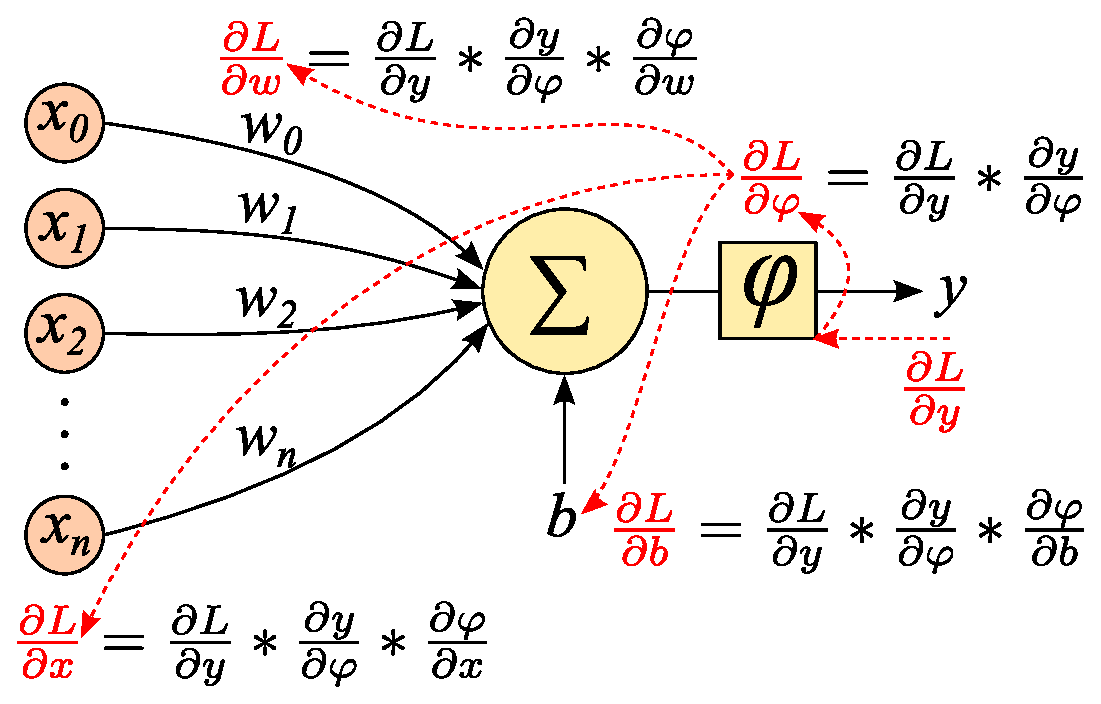
\includegraphics[scale=0.55]{Yapilan-Calismalar/Figures/perceptronDerivative.pdf}
		}
	\end{center}
\end{figure}

Tam bağlantılı katmanlarda eğitim, ağırlık ($W$) ve yanlılık ($b$) parametrelerinde gerçekleştirilmektedir. Çok katmanlı mimarilerin tüm katmanlarında olduğu gibi tam bağlantılı katmanlarda da eğitim ağın genel kayıp fonksiyonunun gradyanı kullanılarak gerçekleştirilmektedir. Bu sebeple güncellenecek tüm eğitilebilir parametrelerde bir sonraki katmandan gelen hata bilgisine $\frac{\partial L}{\partial  y}$ göre zincir kuralı kullanılarak kısmi türevlerin hesaplanması gerekmektedir. Şekil \ref{fig:perceptronDerivative}'da bir sinir hücresinin bir sonraki katmandan gelen $\frac{\partial L}{\partial  y}$ hata bilgisine göre ağırlık ($W$) ve  yanlılık ($b$) bilgilerini eğitim için güncelleştirilmesinde kullanılacak kısmi türev hesabı gösterilmektedir. $x$ giriş ifadelerindeki kısmi türev hesabı ilgili katmanın ara katman olması durumunda hatanın ilk katmanlara iletiminde kullanılması olmaktadır. Eğer kısmi türevi hesaplanan katman giriş katmanı ise $x$ değerleri için hesaplanan değerler kullanılmamaktadır.

Sinir hücresi çıkışı $y$'nin bir sonraki katmandan gelen hataya göre kısmi türevi $\frac{\partial L}{\partial  y}$ olmak üzere $W$ ve $b$ değerlerini eğitebilmek için gerekli kısmi türev bilgisi sırasıyla Eşitlik \ref{eq:wderivative}, \ref{eq:bderivative} ve \ref{eq:xderivative}'de verilmektedir. Ayrıca $x$ girişleri için ilgili katmandan bir önceki katmana iletilecek hatanın kısmi türevi de Eşitlik \ref{eq:xderivative} kullanılarak hesaplanabilmektedir.
\begin{equation}
	\label{eq:wderivative}
	\frac{\partial L}{\partial  w} = \frac{\partial L}{\partial  y}* \frac{\partial y}{\partial  \varphi} * \frac{\partial  \varphi}{\partial  w}
\end{equation}
\vspace{-1cm} 
\begin{equation}
	\label{eq:bderivative}
	\frac{\partial L}{\partial  b} = \frac{\partial L}{\partial  y}* \frac{\partial y}{\partial  \varphi} * \frac{\partial  \varphi}{\partial  b}
\end{equation} 
\vspace{-1cm}
\begin{equation}
	\label{eq:xderivative}
	\frac{\partial L}{\partial  x} = \frac{\partial L}{\partial  y}* \frac{\partial y}{\partial  \varphi} * \frac{\partial  \varphi}{\partial  x}
\end{equation} 

\subsubsection{Konvolüsyon Katmanları}

Konvolüsyonel Sinir Ağları (CNN) en önemli derin öğrenme ağlarından biridir. Bu sinir ağı modelinde konvolüsyon katmanları, girdi olarak verilen sinyal, görüntü ya da 3B volümetrik veriden otomatik özellik çıkarma işlemini gerçekleştirmektedir. Konvolüsyon katmanları el yazısı ile yazılmış zip kodlarını tanımaya yönelik geliştirilen bir çalışmada ilk kez kullanılmıştır \cite{lecun1989backpropagation}.

Konvolüsyon katmanları CNN mimarisinin yapı taşlarıdır. Özellik çıkarımı yapılacak verinin boyutlarına göre yapılandırılabilmektedir. Bu sayede ham veri 1B bir sinyal ise 1B konvolüsyon filtreleri kullanılarak 1B uzayda özellik çıkarma işlemi yapılabilmektedir. Aynı şekilde veri 2B bir görüntü ise 2B konvolüsyon filtreleri kullanılarak 2B uzayda özellik çıkarma işlemi gerçekleştirilebilmektedir. Verinin 3B volümetrik bir veri olması durumunda ise 3B konvolüsyon filtreleri kullanılarak 3B özellik çıkarma işlemi gerçekleştirilebilmektedir. Konvolüsyonel katmanlarda öğrenilen bilgi ham veriye uygulanan konvolüsyon filtrelerinin değerleri olmaktadır. Bu tez çalışmasında tek kanallı laboratuvar görüntüleri kullanıldığı için konvolüsyon işlemi tek kanallı gri seviye görüntüler üzerinde gerçekleştirilmektedir.

$G$ konvolüsyonu hesaplanacak görüntü, $F$ konvolüsyon filtresi, $i$ değeri görüntünün $x$ yatay eksendeki indeksi, $j$ değeri görüntünün $y$ dikey eksendeki indeksi olmak üzere $O$ konvolüsyon işlemi sonucu ortaya çıkacak özellik haritası Eşitlik \ref{eq:konvolusyon}'deki gibi hesaplanmaktadır.
\begin{equation}
	\label{eq:konvolusyon}
	O(i, j)=(F * G)(i, j)=\sum_{m} \sum_{n} G(i-m, j-n) F(m, n)
\end{equation}

Konvolüsyon işlemi 1B, 2B ve 3B filtreler kullanılarak mevcut işlenecek veriye göre özelleştirilebilmektedir. Konvolüsyon katmanı ile istenen sayıda ve ebatlarda konvolüsyon filtreleri seçilebilmektedir. Ayrıca konvolüsyon filtrelerinin görüntüye uygulanma sırasında Adım Kaydırma (Stride) miktarı da özelleştirilebilmektedir. Konvolüsyon işlemi sonucunda ortaya çıkan özellik haritalarının ebatları herhangi bir Dolgulama (Padding) işlemi gerçekleştirilmediğinde konvolüsyon filtresinin ebatlarına bağlı olarak küçülmektedir. Şekil \ref{fig:conv2d}'de örnek bir 2B görüntü için filtre sayısı 1 ve dolgulama miktarı 0 seçildiğinde konvolüsyon işleminin ilk üç adımı sırasıyla yeşil, mavi ve kırmızı renklerde gösterilmektedir. Adım kaydırma miktarının konvolüsyon işlemi üzerindeki etkisi de yine bu görselde vurgulanmaktadır. Şekil \ref{fig:conv2d}'de görüldüğü gibi adım kaydırma miktarının değişimi elde edilen özellik haritasının ebatlarını direkt belirleyen faktörlerden biridir. 

\captionsetup[figure]{margin={0.3cm,0cm}}
\begin{figure}[h!]
	\begin{center}
		\vspace{0.4cm}
		\captionbox{Filtre sayısı 1 ve dolgulama miktarı 0 seçildiğinde 2B konvolüsyon ve adım kaydırma işlemleri. \label{fig:conv2d}}
		{
			\vspace{0.4cm}
			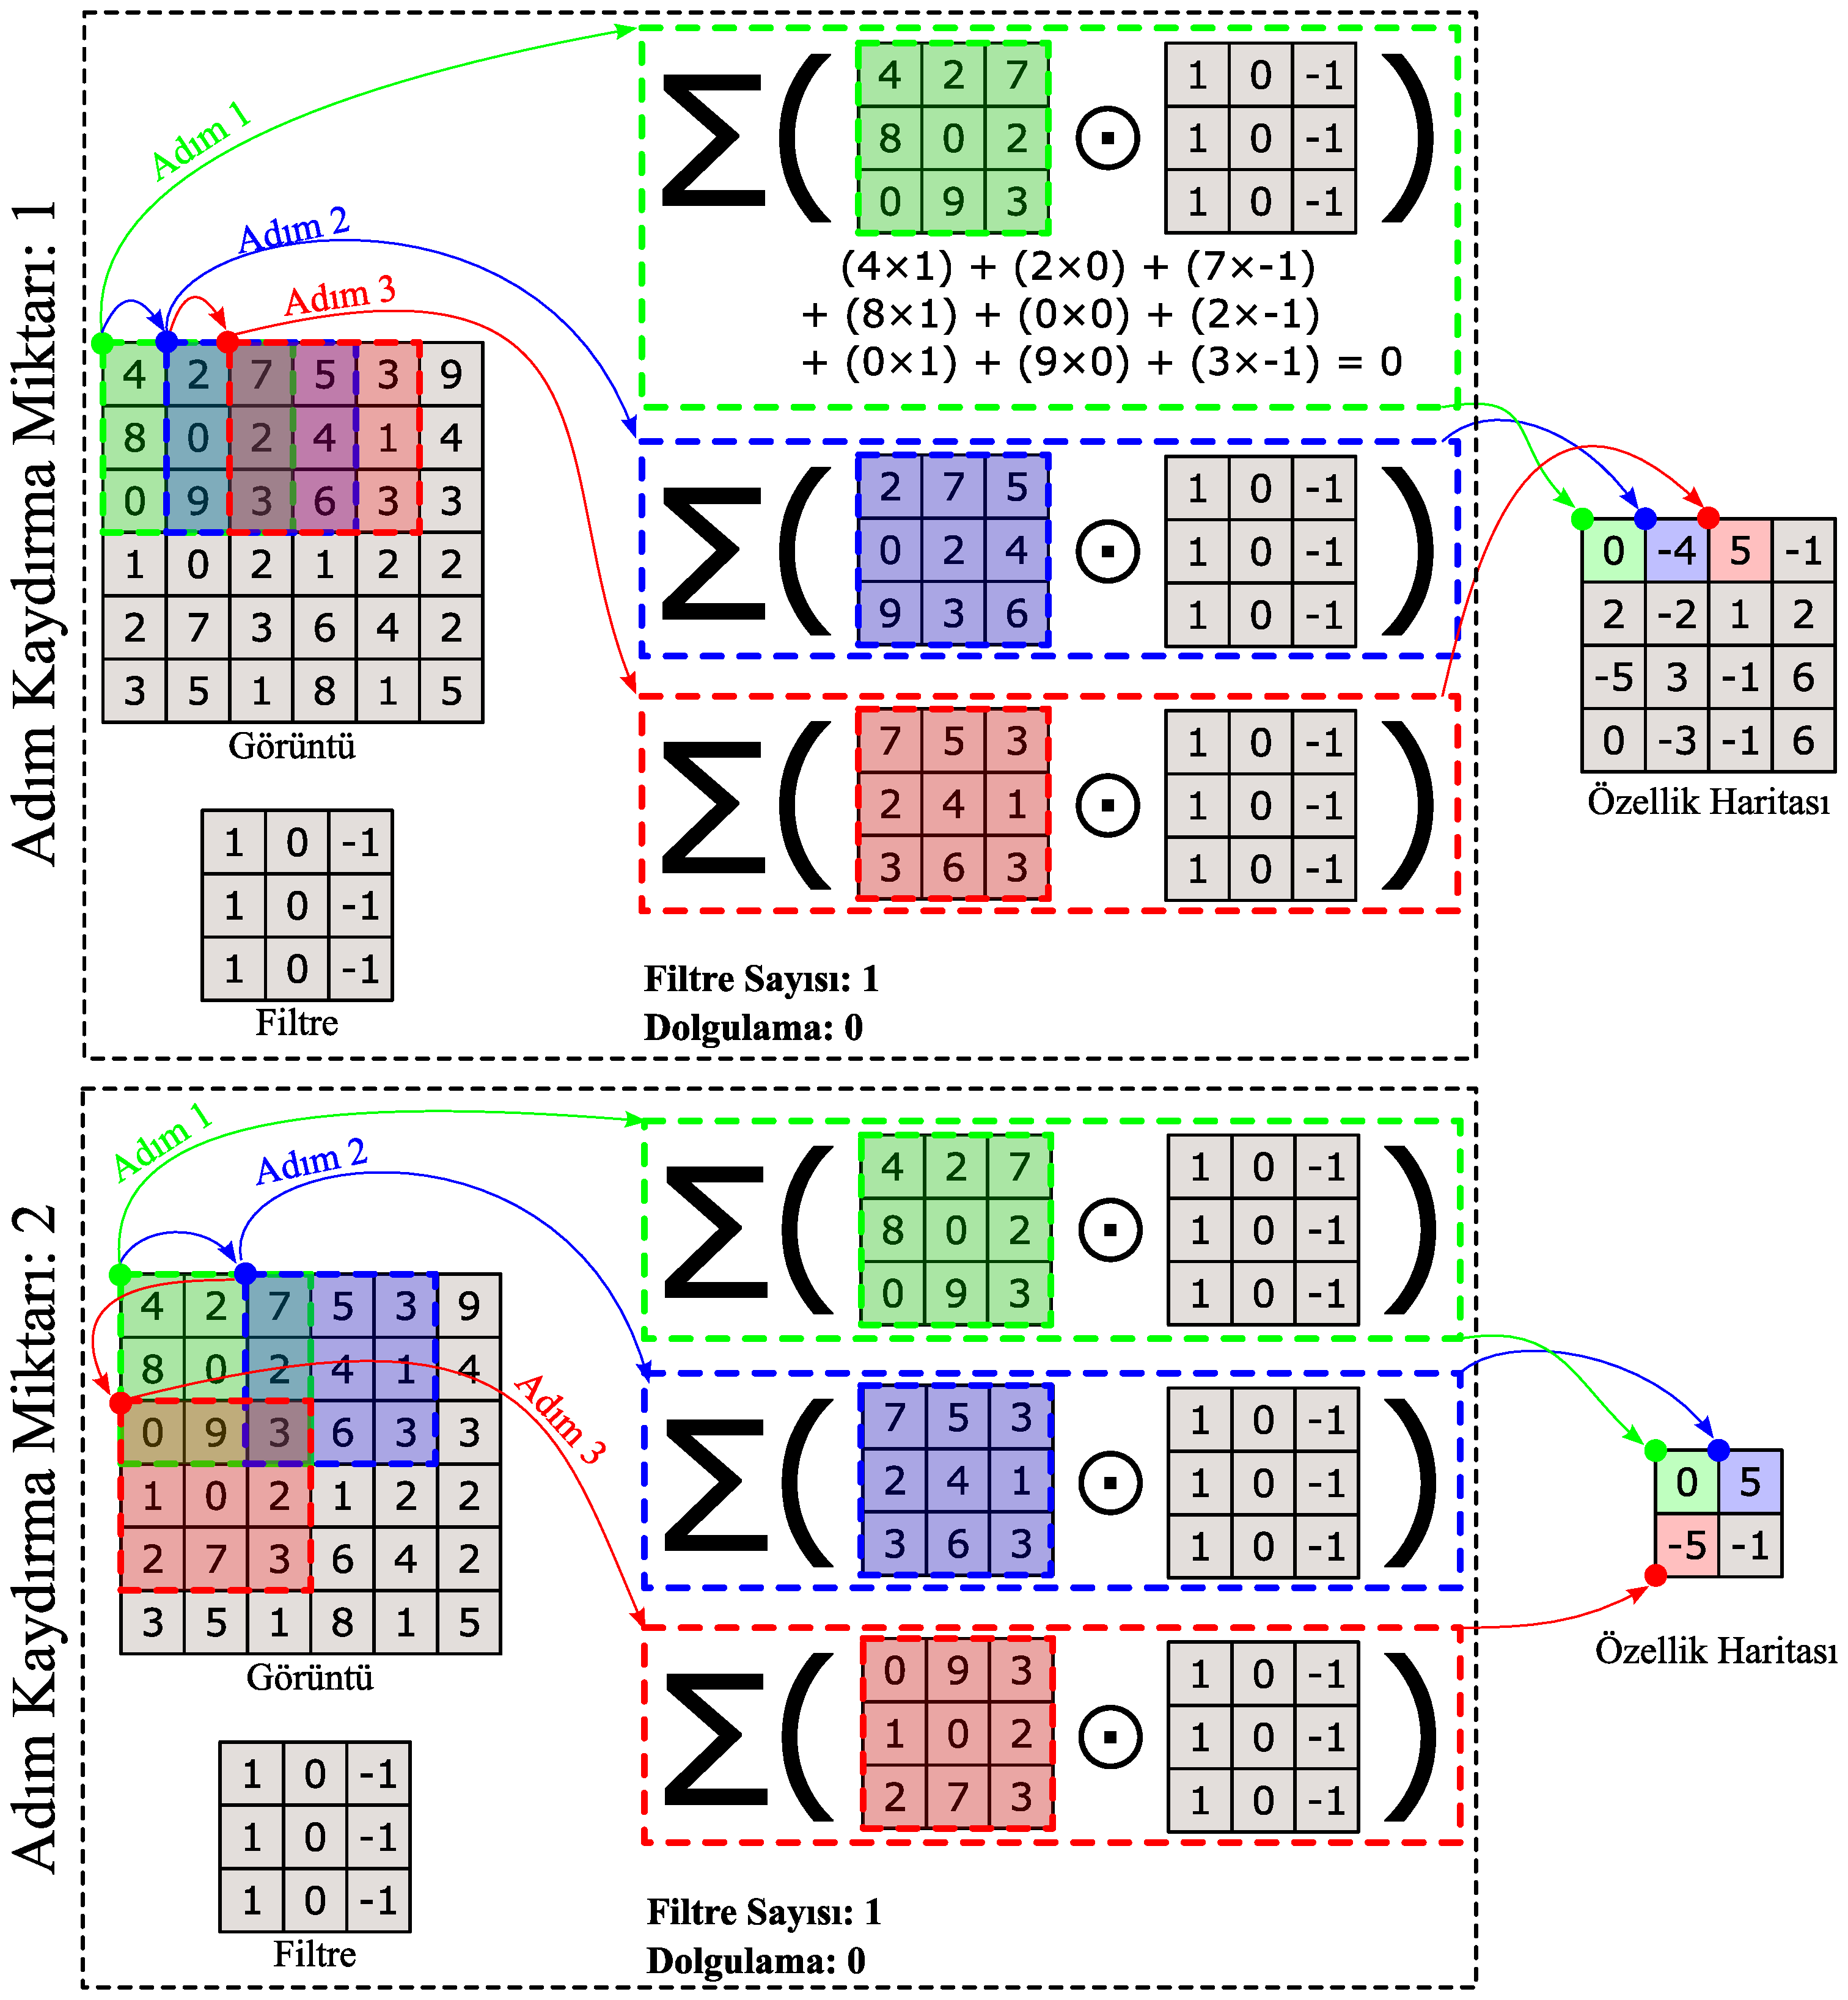
\includegraphics[scale=0.3]{Yapilan-Calismalar/Figures/conv2D2.pdf}
		}
	\end{center}
\end{figure}

Konvolüsyon filtrelerinin sayısı Şekil \ref{fig:conv_sizes}'de gösterildiği gibi konvolüsyon işlemi sonucu ortaya çıkacak özellik haritalarının sayısı ile eşit olmaktadır. Bunun sebebi giriş görüntüsüne konvolüsyon filtrelerinin birbirinden bağımsız uygulanması ve her konvolüsyon filtresinin yeni bir özellik haritası çıkarmasıdır. Ayrıca herhangi bir dolgulama işlemi gerçekleştirilmediğinde konvolüsyon filtrelerinin ebatlarına bağlı olarak hesaplanan özellik haritalarının ebatları giriş görüntüsünden farklı olmaktadır. 

\captionsetup[figure]{margin={0.3cm,-0.2cm}}
\begin{figure}[h!]
	\begin{center}
		\vspace{0.4cm}
		\captionbox{Konvolüsyon işlemi sonrası filtre sayısına bağlı olarak ortaya çıkan özellik haritaları. \label{fig:conv_sizes}}
		{
			\vspace{0.4cm}
			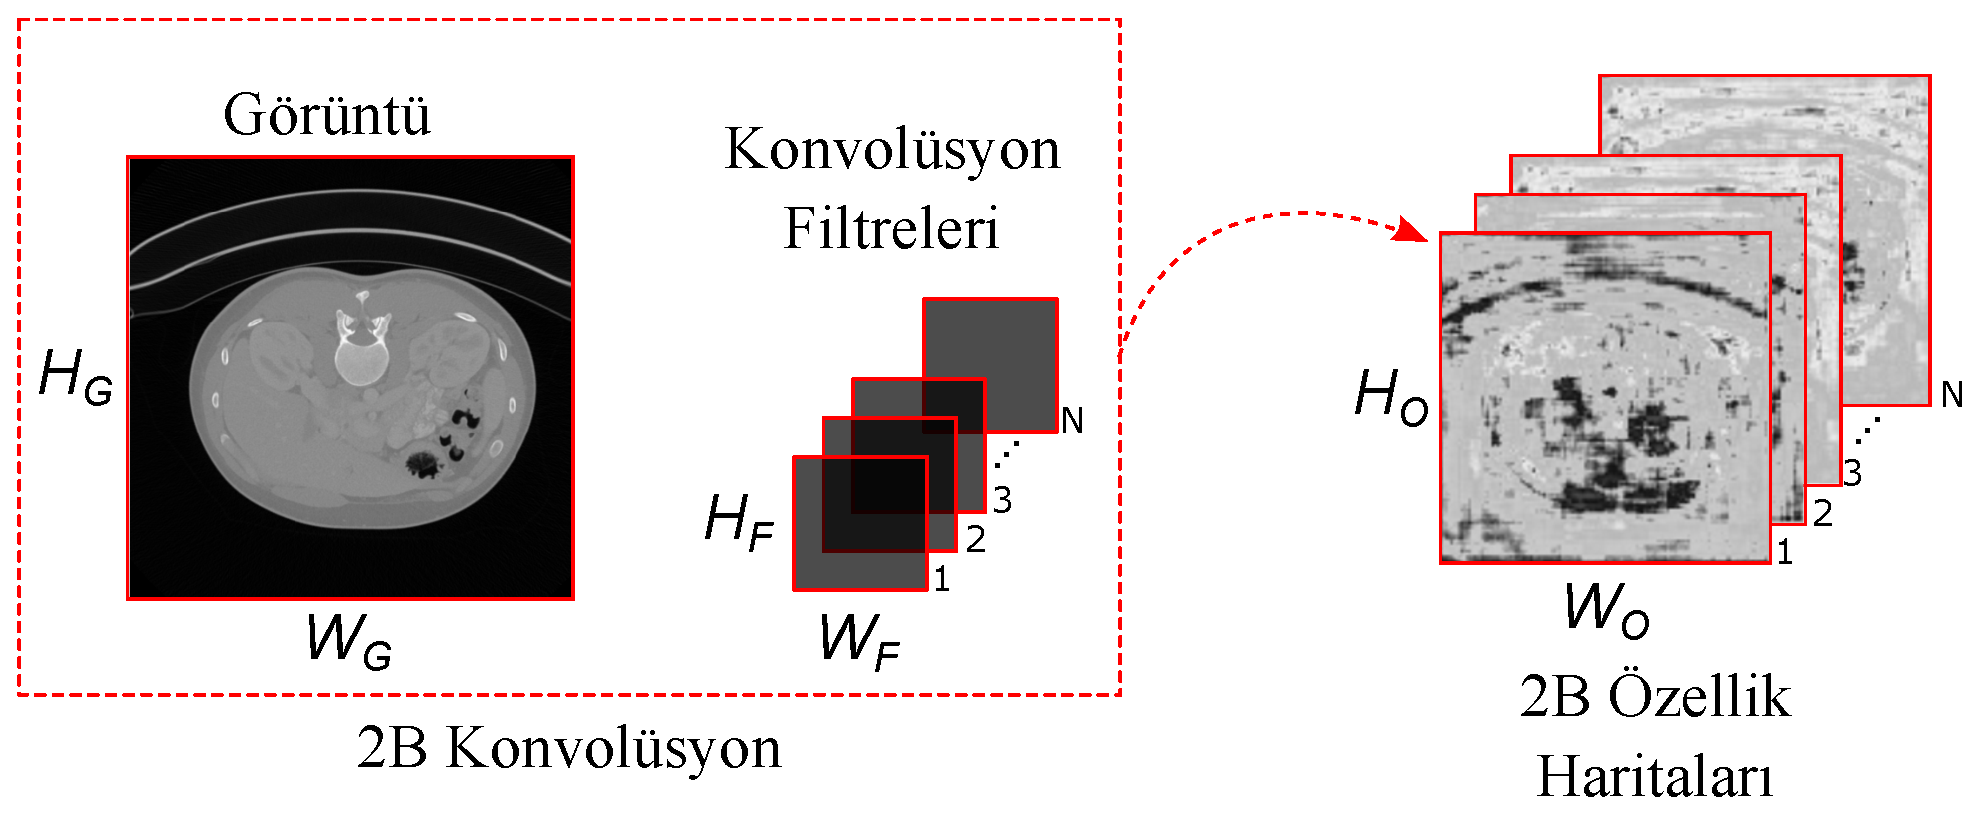
\includegraphics[scale=0.44]{Yapilan-Calismalar/Figures/conv_sizes.pdf}
		}
	\end{center}
\end{figure}

Konvolüsyon işleminde giriş görüntüsünün genişliği $W_{G}$, yüksekliği $H_{G}$, konvolüsyon filtrelerinin genişliği $W_{F}$, yüksekliği $H_{F}$, konvolüsyon işlemi sırasında konvolüsyon filtresinin adım kaydırma miktarı $s$ ve dolgulama miktarı $p$, hesaplanacak özellik haritalarının genişliği $W_{O}$, yüksekliği $H_{O}$ olmak üzere, bu tez çalışmasında kullanılan veri setlerinde giriş verisinin genişlik ve yükseklik değerlerinin eşit uzunlukta olması ve eşit uzunluklu filtreler tercih edildiğinden dolayı giriş verisi ebatları $W_{G}=H_{G}=G$, konvolüsyon filtresi ebatları $W_{F}=H_{F}=F$ olarak kabul edilirse çıkış özellik haritasının ebatları $W_{O}=H_{O}=O$ Eşitlik \ref{eq:featuremapsize}'daki gibi hesaplanabilmektedir.
\begin{equation}
	\label{eq:featuremapsize}
	O=\left\lfloor \frac{G-F+2p}{s}+1 \right\rfloor
\end{equation}

Bu çalışmada 2B konvolüsyon işlemleri gerçekleştirildiği gibi 3B konvolüsyon işlemleri de gerçekleştirilmektedir. 3B konvolüsyon işleminde giriş görüntüleri 3B volümetrik verilerden oluşmaktadır. Bu volümetrik verilere konvolüsyon işlemi 3B konvolüsyon filtreleri ile 2B konvolüsyon işleminde olduğu gibi adım kaydırma ve dolgulama işlemleri ile uygulanabilmektedir. 3B volümetrik görüntülerde 3B konvolüsyon filtrelerinin gezdirilmesine yönelik görsel Şekil \ref{fig:conv3d}'da gösterilmektedir.

\captionsetup[figure]{margin={0.5cm,-2.2cm}}
\begin{figure}[h!]
	\begin{center}
		\vspace{0.4cm}
		\captionbox{3B volümetrik görüntülerde 3B konvolüsyon filtrelerinin gezdirilmesi.\label{fig:conv3d}}
		{
			\vspace{0.4cm}
			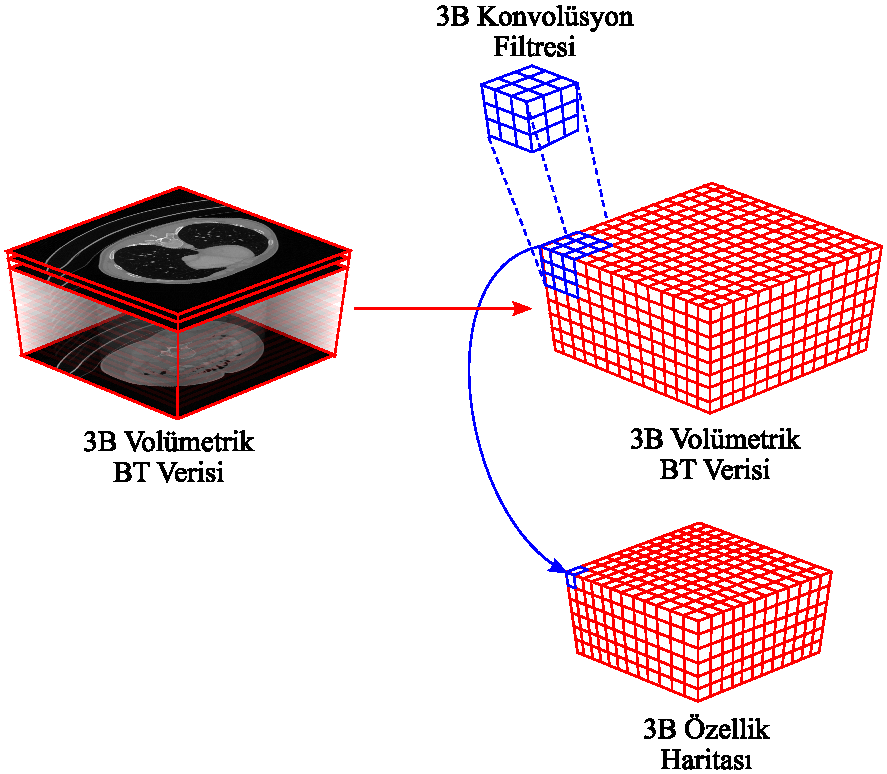
\includegraphics[scale=0.7]{Yapilan-Calismalar/Figures/conv3D.pdf}
		}
	\end{center}
\end{figure}

Konvolüsyon işleminde hesaplanan özellik haritalarının ebatlarının giriş görüntü ebatları ile aynı olmasının istenildiği durumlarda dolgulama işlemi gerçekleştirilmektedir. 2B görüntüde dolgulama işlemi gerçekleştirerek konvolüsyon özellik haritası hesaplama işlemi Şekil \ref{fig:conv2Dpadding}'da gösterilmektedir. Görüldüğü gibi giriş görüntüsü $0$ değerli bir çerçeve içerisine alınarak konvolüsyon işlemi gerçekleştirilmektedir. Özellikle konvolüsyon filtrelerinin ebatları büyüdüğünde görüntüden hesaplanan özellik haritalarının ebatları oldukça düşmektedir. Dolgulama işlemi ile bu problem büyük ölçüde ortadan kaldırılabilmektedir.

\captionsetup[figure]{margin={0.2cm,-3cm}}
\begin{figure}[h!]
	\begin{center}
		\vspace{0.4cm}
		\captionbox{2B konvolüsyon işleminde dolgulama işlemi.\label{fig:conv2Dpadding}}
		{
			\vspace{0.4cm}
			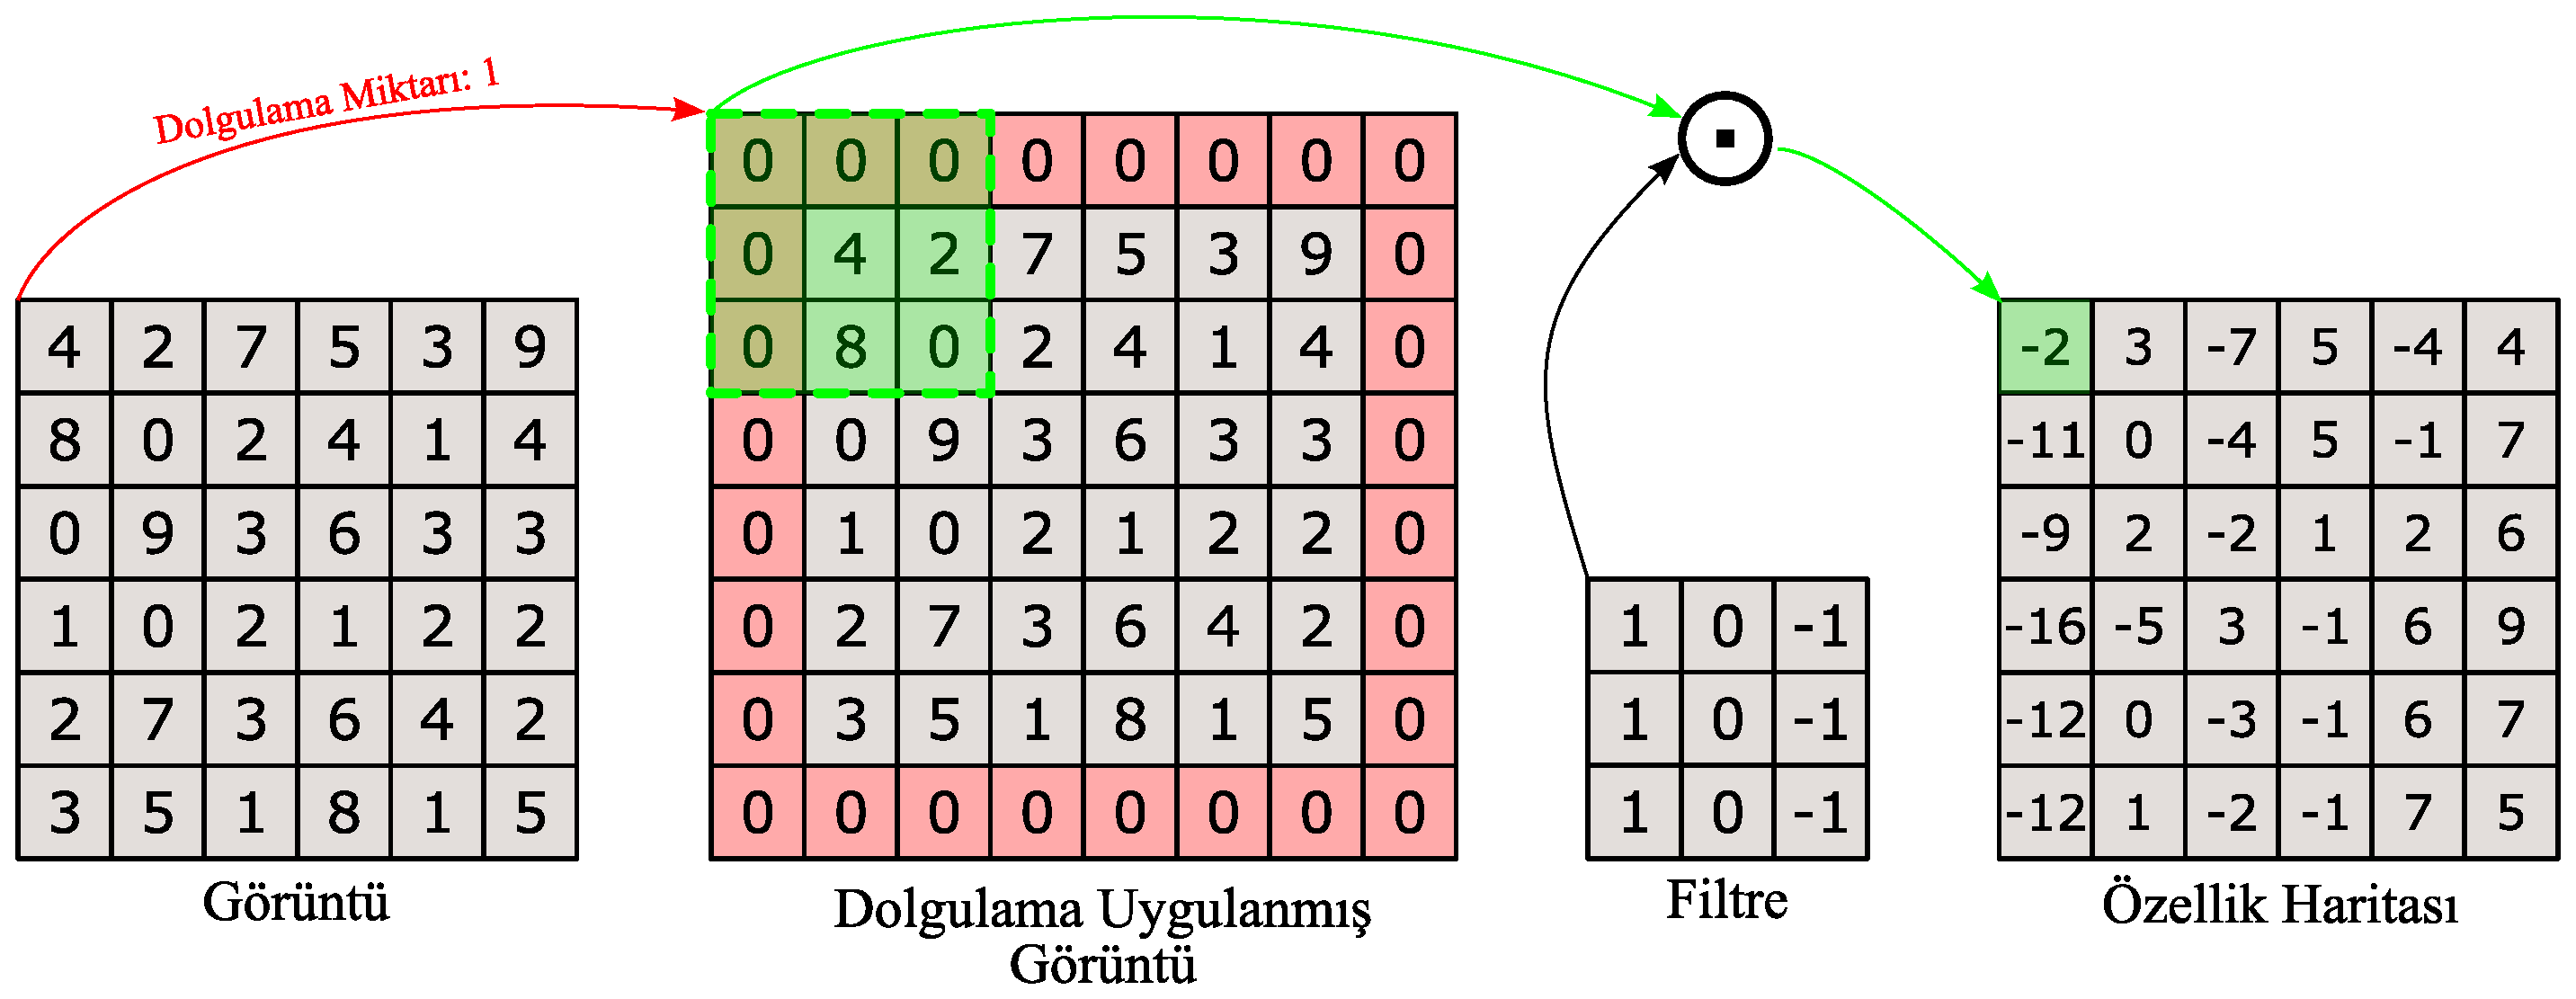
\includegraphics[scale=0.32]{Yapilan-Calismalar/Figures/conv2Dpadding.pdf}
		}
	\end{center}
\end{figure}

Konvolüsyon işleminde dolgulama miktarı $p$, filtre ebatları $F$ olmak üzere dolgulama miktarı Eşitlik \ref{eq:padding}'daki gibi hesaplanabilmektedir.
\begin{equation}
	\label{eq:padding}
	p=\frac{F-1}{2}
\end{equation}

Konvolüsyon katmanlarında eğitim $F$ filtre parametreleri üzerinde gerçekleştirilmektedir. Tüm diğer katmanlarda olduğu gibi konvolüsyon katmanında da eğitim gerçekleştirebilmek için modelin genel hatasının zincir kuralına göre gradyanının hesaplanılması gerekmektedir. Konvolüsyon katmanına uygulanan giriş verisi $G$ ve konvolüsyon katmanının çıkışı $O$ olmak üzere bir sonraki katmandan gelen hatanın kısmi türevi $\frac{\partial L}{\partial  O}$ ile $F$ filtre parametrelerini güncellemek için hesaplanılması gereken $\frac{\partial L}{\partial  F}$ kısmi türevinin zincir kuralına göre geri yayılımı Şekil \ref{fig:convDerivative}'de gösterilmektedir. Bu kısmi türev Eşitlik \ref{eq:convFderivative} kullanılarak hesaplanmaktadır.
\begin{equation}
	\label{eq:convFderivative}
	\frac{\partial L}{\partial  F} = \frac{\partial L}{\partial  O}* \frac{\partial O}{\partial  F}
\end{equation}

\captionsetup[figure]{margin={0.2cm,-3cm}}
\begin{figure}[h!]
	\begin{center}
		\vspace{0.4cm}
		\captionbox{Hatanın geri yayılımı ile konvolüsyon katmanının kısmi türevleri.\label{fig:convDerivative}}
		{
			\vspace{0.4cm}
			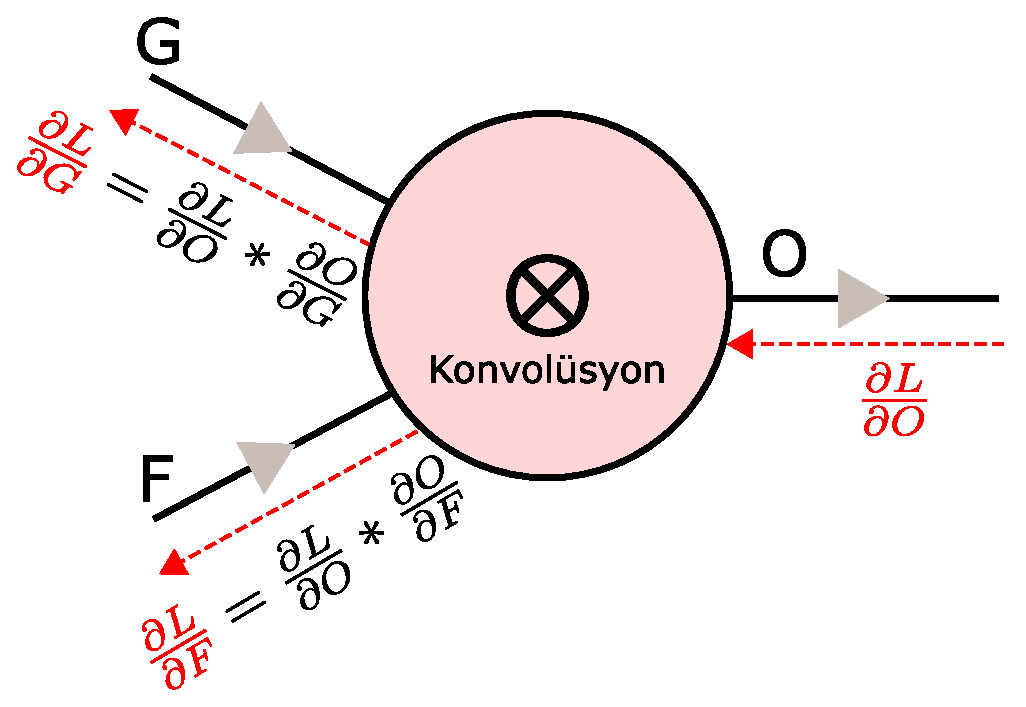
\includegraphics[scale=0.6]{Yapilan-Calismalar/Figures/convDerivative.pdf}
		}
	\end{center}
\end{figure}

İlgili konvolüsyon katmanından önceki katmanlara hatanın yayılımı $G$ görüntü girişi yönündeki $\frac{\partial L}{\partial  G}$ kısmi türevi Eşitlik \ref{eq:convGderivative} kullanılarak hesaplanmaktadır. Önceki katmanlardaki zincir kuralına benzer şekilde uygulanarak eğitilebilir parametrelerin güncellenmesi sağlanmaktadır.
\begin{equation}
	\label{eq:convGderivative}
	\frac{\partial L}{\partial  G} = \frac{\partial L}{\partial  O}* \frac{\partial O}{\partial  G}
\end{equation}


\subsubsection{Ters Konvolüsyon Katmanları}

Konvolüsyon katmanları dolgulama yapılmadığı taktirde girişlerinden uygulanan verilerden özellik çıkarırlarken giriş verisi boyutları küçültülmektedir. Özellikle oto-kodlayıcılarda bu boyut küçültme işlemi kodlama işlemi olarak adlandırılmaktadır. Oto-kodlayıcıların girişinden uygulanan verilerde gürültü azaltma, görüntü bölütleme v.b. işlemler gerçekleştirebilmektedir. Oto-kodlayıcılarda hiyerarşik olarak giriş verisi boyutları küçültülerek kodlama işlemi yapılmakta ve girişten uygulanan verinin kompleks özellik haritaları elde edilmektedir. Bu özellik haritalarından ters yönde hiyerarşik olarak boyut artırarak giriş verisiyle eşit boyutlarda görüntüler elde edebilmek için ters konvolüsyon katmanları kullanılabilmektedir. Dolayısıyla ters konvolüsyon katmanları genellikle konvolüsyon katmanlarından sonra hesaplanan özellik haritalarının eski boyutlarına getirilmesinde kullanılmaktadır.

\captionsetup[figure]{margin={0.5cm,-0.5cm}}
\begin{figure}[h!]
	\begin{center}
		\vspace{0.4cm}
		\captionbox{Adım kaydırma miktarı 1, Filtre sayısı 1 ve dolgulama miktarı 0 seçildiğinde 2B Ters Konvolüsyon işlemi.\label{fig:conv2Dtranspose1}}
		{
			\vspace{0.4cm}
			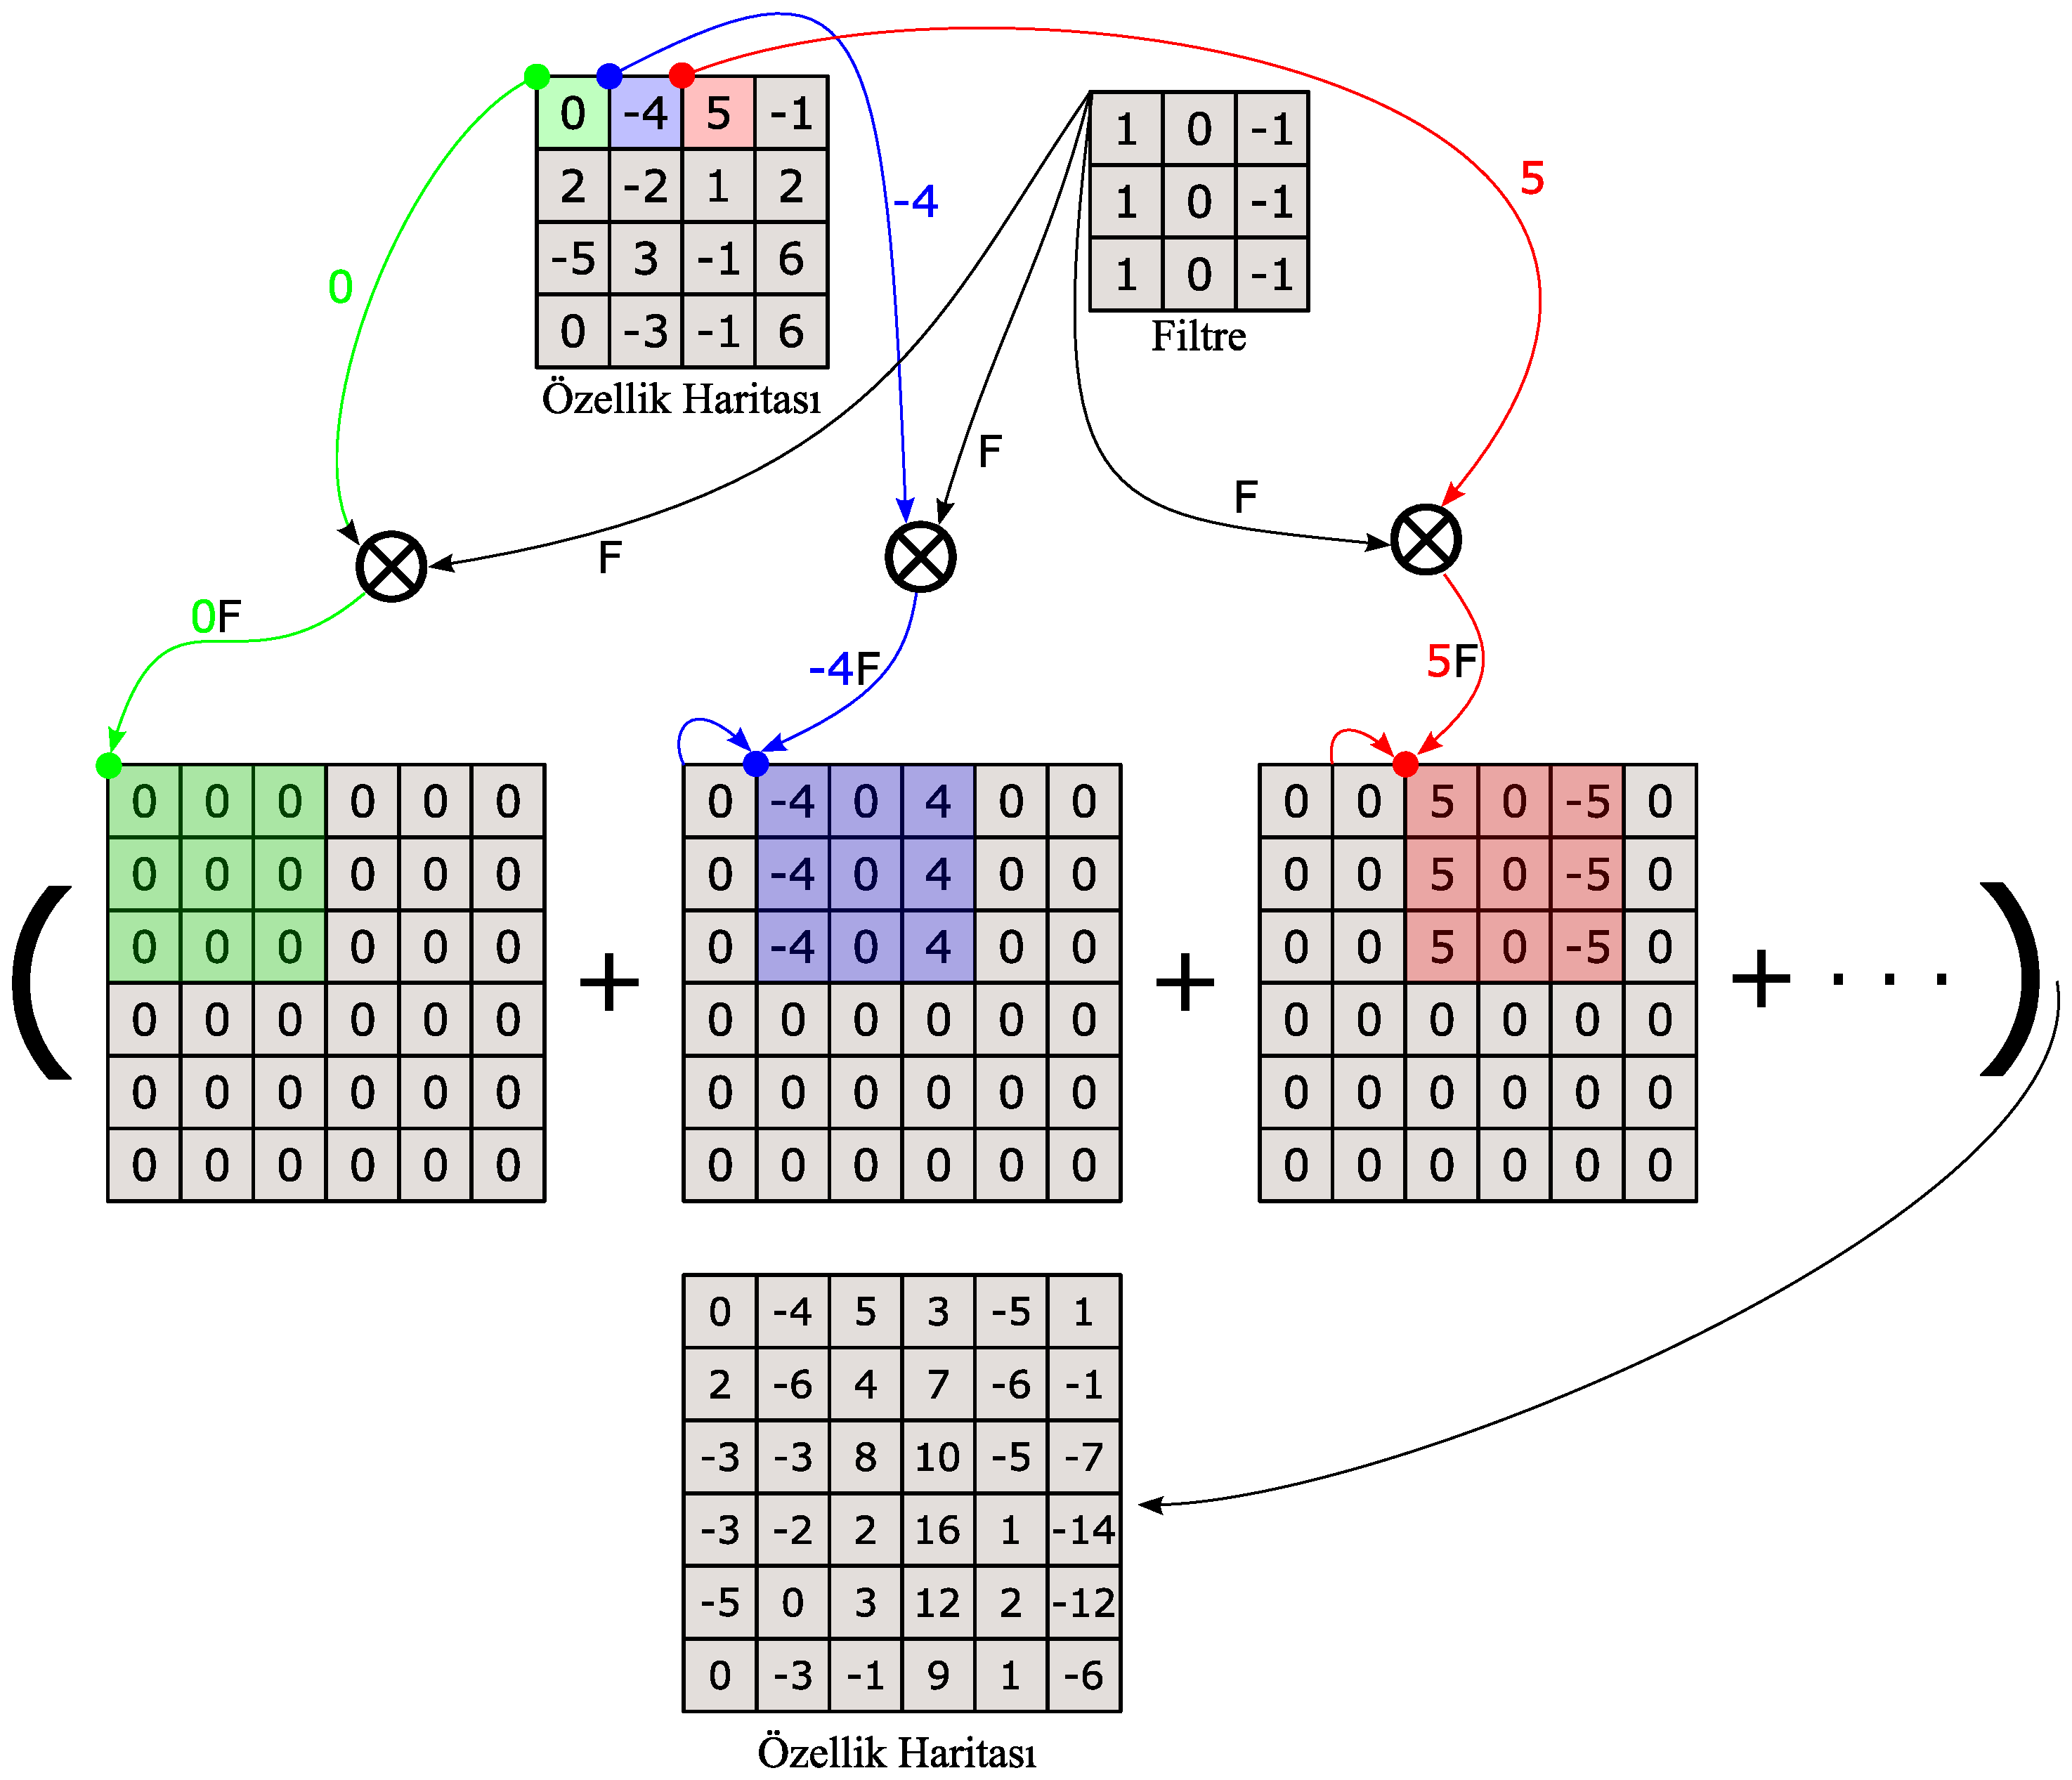
\includegraphics[scale=0.28]{Yapilan-Calismalar/Figures/conv2Dtranspose1.pdf}
		}
	\end{center}
\end{figure}

Ters konvolüsyon işleminde öncelikle ters konvolüsyon sonrası ortaya çıkacak özellik haritasının boyutlarını belirlemek gerekmektedir. Konvolüsyon işlemi sonucunda girişten uygulanan verinin boyutları küçültülürken, ters konvolüsyon işleminde girişten uygulanan verinin boyutları büyütülmektedir. Ters konvülüsyon işleminde giriş özellik haritasının ebatları $G$, filtre ebatları $F$, dolgulama miktarı $p$, adım kaydırma miktarı $s$ olmak üzere çıkış $O$ özellik haritasının ebatları Eşitlik \ref{eq:convtrans} kullanılarak hesaplanabilmektedir. Bu eşitlikte $\alpha$ katsayısı ters konvolüsyon işleminde görüntü ebatlarının istenen ebatlara ölçeklenebilmesi için kullanıcı tanımlı hiper parametredir. $\alpha$ parametresine adım kaydırma miktarı $s=1$ değerinden farklı olduğunda ihtiyaç duyulmaktadır.
\begin{equation}
	\label{eq:convtrans}
	O=s(G-1)+\alpha+k-2p \text{ , } \alpha\in\left\{ 0,...,s-1 \right\}
\end{equation}

\captionsetup[figure]{margin={0.4cm,-0.8cm}}
\begin{figure}[h!]
	\begin{center}
		\vspace{0.4cm}
		\captionbox{Adım kaydırma miktarı 2, Filtre sayısı 1 ve dolgulama miktarı 0 seçildiğinde 2B Ters Konvolüsyon işlemi.\label{fig:conv2Dtranspose2}}
		{
			\vspace{0.4cm}
			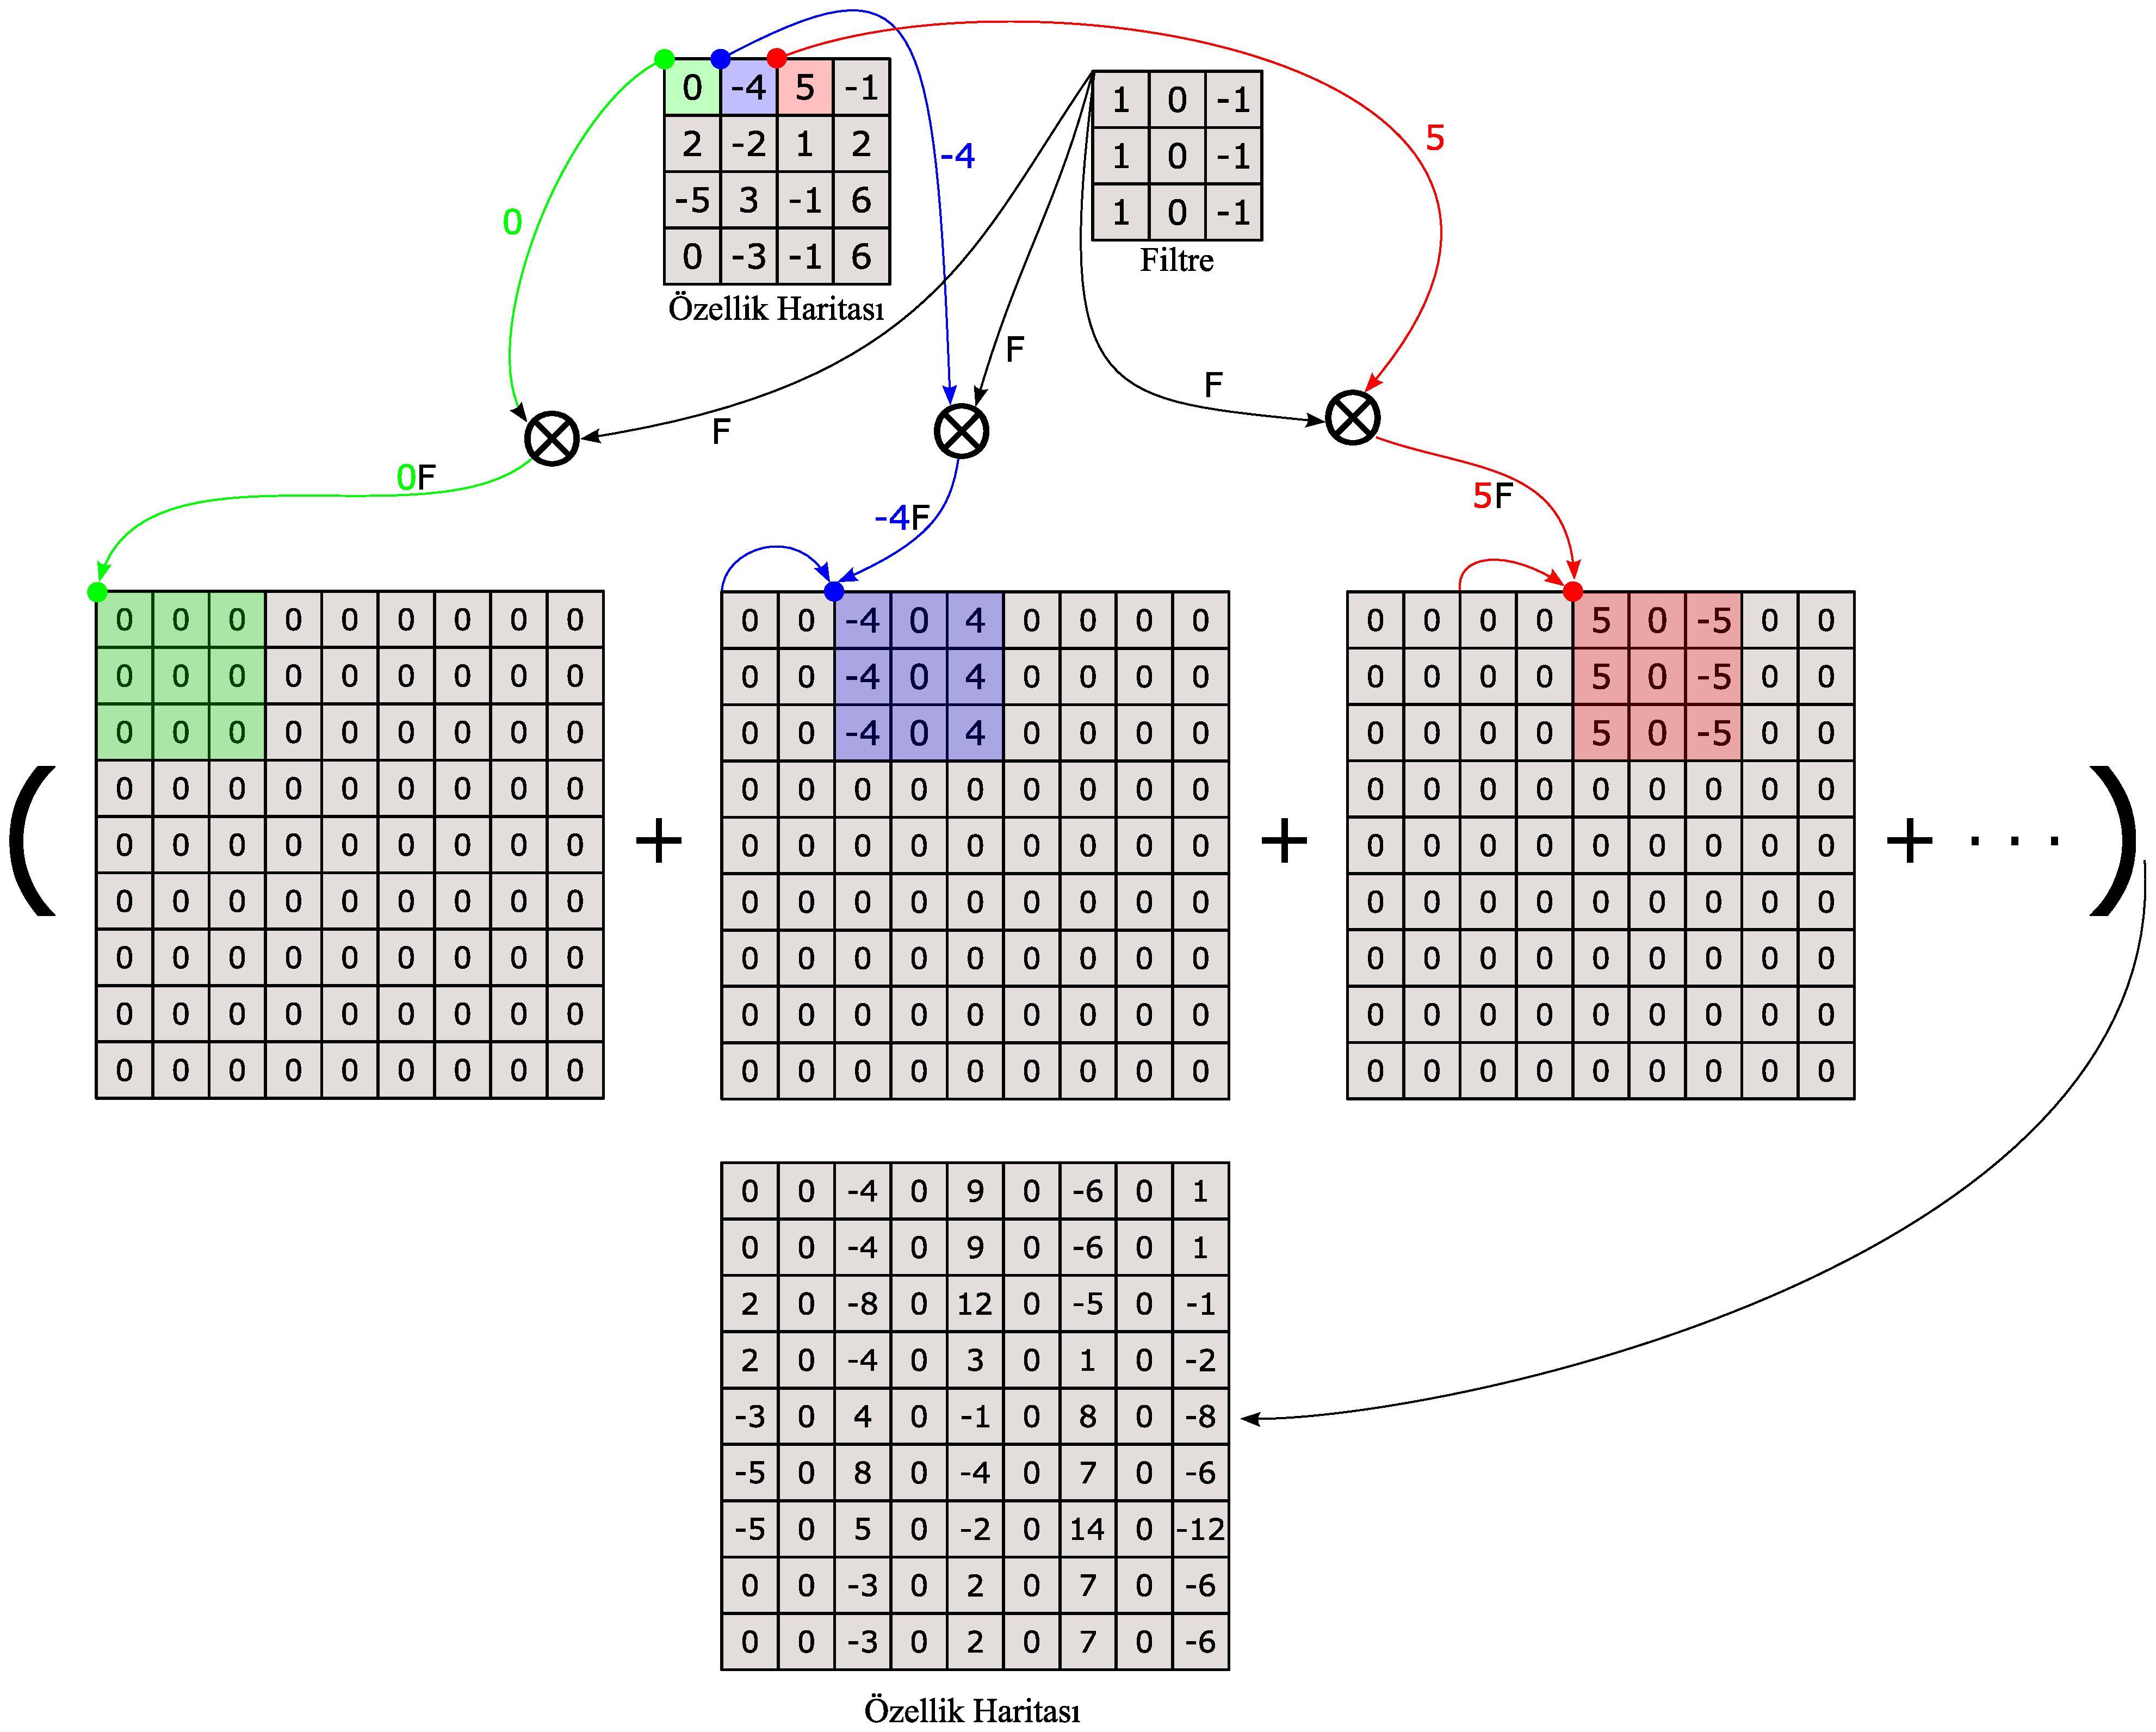
\includegraphics[scale=0.2]{Yapilan-Calismalar/Figures/conv2Dtranspose2.pdf}
		}
	\end{center}
\end{figure}

Ters konvolüsyon işleminde dolgulama konvolüsyon işleminin tersi mantığında çalışmaktadır. Eğer dolgulama miktarı $0$ olarak seçilirse Şekil \ref{fig:conv2Dtranspose1}'de görüldüğü gibi giriş görüntüsüne boyut artırma işlemi gerçekleştirilmektedir. Görüldüğü gibi boyut artırma miktarı Şekil \ref{fig:conv2d}'deki konvolüsyon işlemi öncesindeki giriş verisinin boyutlarına eşit olmaktadır. Bu özellik segmentasyon aşamasında ardışık özellik çıkarma aşamalarından sonra segmente edilmiş ve giriş görüntüsüyle eşit boyutlarda özellik haritaları elde etmemizi sağlamaktadır.

Ters konvolüsyon işleminde adım miktarının artırılması ise yine konvolüsyon işleminin ters yönünde boyutu artırmaktadır. Ters konvolüsyon işleminde adım miktarı konvolüsyon işleminde uygulanan adım miktarı ile eşdeğer seçilerek konvolüsyon işlemi ile kaybedilen özellik haritası ebatlarının geri kazanılmasını sağlayabilmektedir. Şekil \ref{fig:conv2Dtranspose2}'te görüldüğü gibi adım sayısının artırılması ters konvolüsyon işlemi sonrasında elde edilen özellik haritalarının ebatlarının büyümesini sağlamaktadır.

Dolgulama miktarı ise yine konvolüsyon işlemindeki dolgulamanın aksine kırpma işlemi gerçekleştirmektedir. Dolgulama miktarı konvolüsyon işleminde olduğu gibi Eşitlik \ref{eq:padding} kullanılarak hesaplanmaktadır. Hesaplanan dolgulama miktarı kadar pikseller Şekil \ref{fig:conv2Dtrpadding}'te gösterildiği gibi nihai ters konvolüsyon özellik haritasından kırpılmaktadır.

\captionsetup[figure]{margin={0.4cm,-0.2cm}}
\begin{figure}[h!]
	\begin{center}
		\vspace{0.4cm}
		\captionbox{2B konvolüsyon işleminde dolgulama.\label{fig:conv2Dtrpadding}}
		{
			\vspace{0.4cm}
			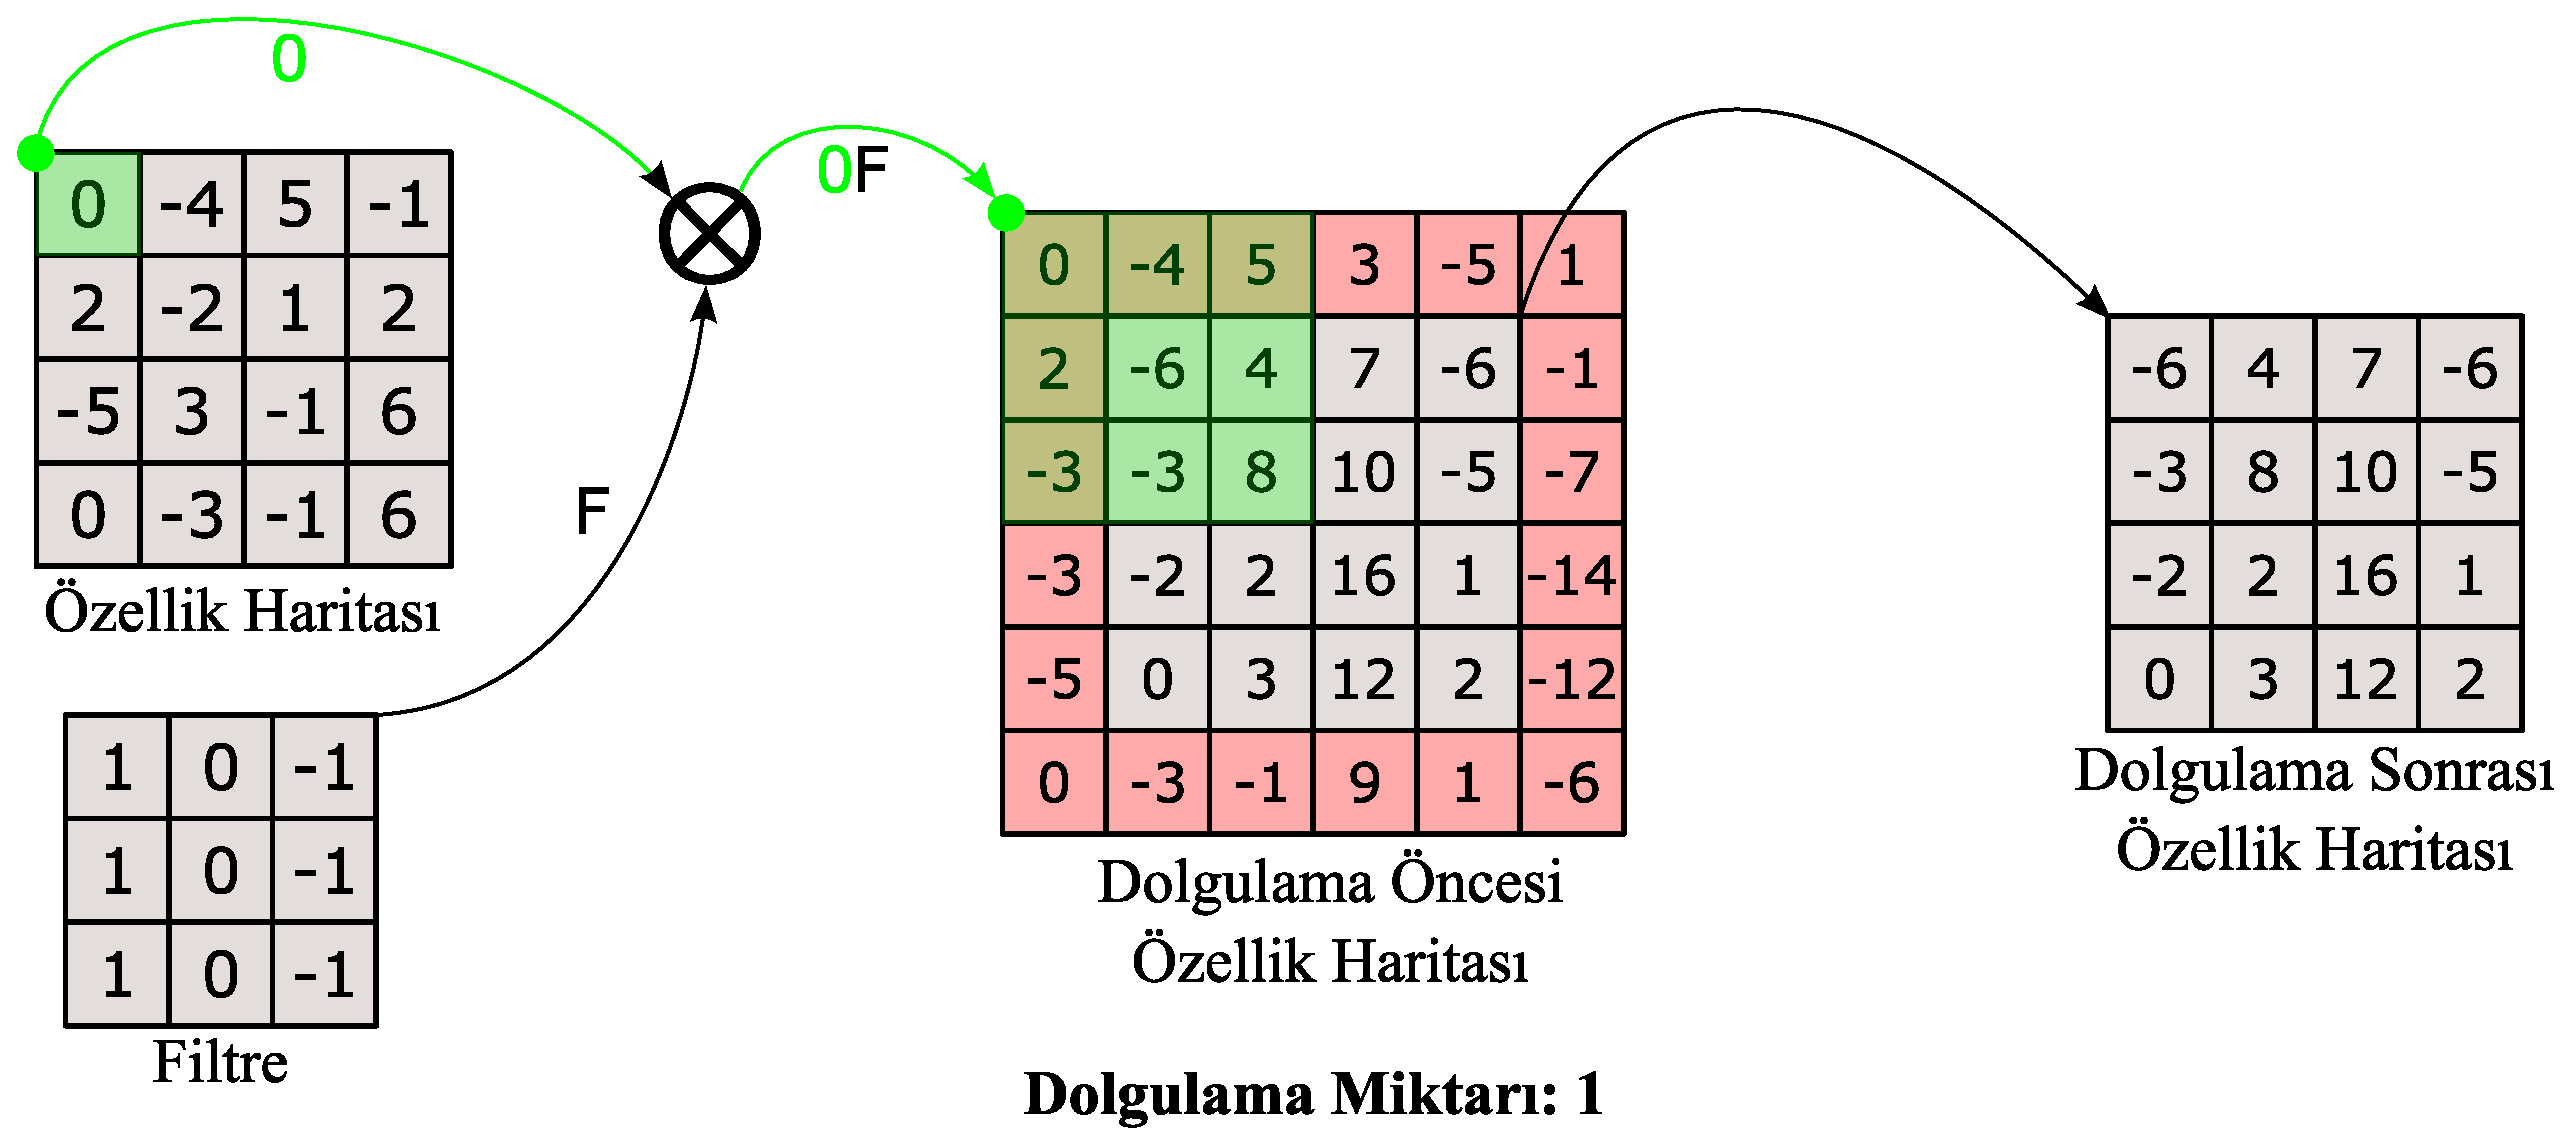
\includegraphics[scale=0.3]{Yapilan-Calismalar/Figures/conv2Dtrpadding.pdf}
		}
	\end{center}
\end{figure}

Ters konvolüsyon katmanlarının eğitimi konvolüsyon katmanlarına benzer şekilde gerçekleştirilmektedir. Konvolüsyon katmanında olduğu gibi girişine $G$ giriş verisi uygulanan $F$ eğitilebilir filtre parametrelerine sahip ters konvolüsyon katmanının çıkışı $O$ olmak üzere, $F$ filtre parametrelerini güncellemek için gerekli ağın genel hatasının gradyanının geri yayılım algoritmasının zincir kuralına göre Eşitlik \ref{eq:convFderivative}'den elde edilen kısmi türev ile gerçekleştirilmektedir. Ters konvolüsyon katmanından önceki katmanlara ise bu gradyan bilgisi Eşitlik \ref{eq:convGderivative} ile aktarılmaktadır.
 
\subsubsection{Aktivasyon Katmanları}
Aktivasyon katmanları eğitilebilir katmanların hemen ardından eklenerek peşine eklendiği katmanın doğrusallıktan kurtulmasını sağlamaktadır. Doğrusal bir öğrenme 2B hiperdüzlemde birinci dereceden bir eğri çizmeyi sağlayabilmektedir. Oysaki gerçek hayat problemlerini sınıflandırabilmek için doğrusal ayıraçlar kullanmak Şekil \ref{fig:lineer_nonlineer}'te görüldüğü gibi veriyi verimsiz sınıflandırmaya sebep olmaktadır.

\captionsetup[figure]{margin={0.4cm,-3cm}}
\begin{figure}[h!]
	\begin{center}
		\vspace{0.4cm}
		\captionbox{Doğrusal ve doğrusal olmayan aktivasyon fonksiyonları ile verinin sınıflandırılması.\label{fig:lineer_nonlineer}}
		{
			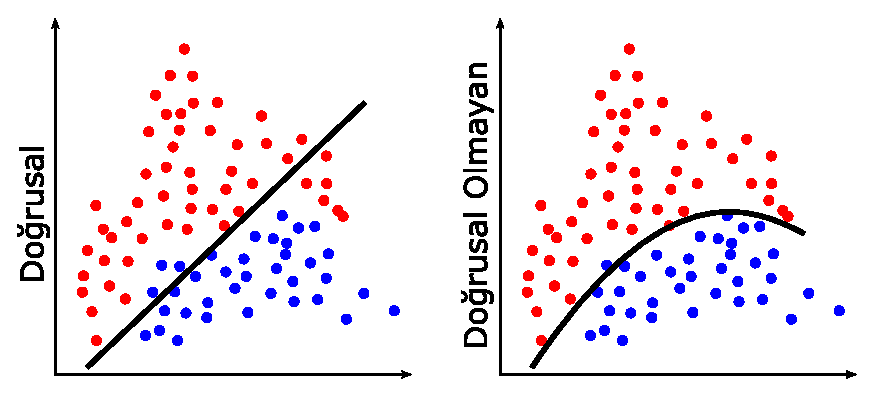
\includegraphics[scale=0.64]{Yapilan-Calismalar/Figures/lineer_nonlineer.pdf}
		}
	\end{center}
\end{figure}

Derin öğrenme modellerinde geri yayılım algoritması için gradyan tabanlı optimizasyon teknikleri kullanıldığından eğitim aşamasında zincir kuralına göre türevi kolay hesaplanabilen bir aktivasyon fonksiyonu tercih etmek hesaplama kolaylığı sağlamaktadır.
\vspace{0.2cm}

\begin{itemize}
    \item Doğrusal Aktivasyon Fonksiyonu:
    
    Doğrusal aktivasyon fonksiyonu ileri yönde hesaplama yapıldığında bir önceki katmandan gelen çıkış ifadesinin Eşitlik \ref{eq:lineer_activ}'te gösterildiği gibi değiştirilmeden kullanıldığı aktivasyon fonksiyonudur.
    {\setlength{\mathindent}{0cm}
    \begin{equation}
    	\label{eq:lineer_activ}
    	f(x)=O=x
    \end{equation}
    \vspace{-1.5cm}
    \begin{equation}
    	\label{eq:dlineer_activ}
    	f^{\prime}(x)=\frac{\partial L}{\partial  O}=1
    \end{equation}}    
    Doğrusal aktivasyon fonksiyonu Eşitlik \ref{eq:dlineer_activ}'te gösterildiği gibi türevi sabit (1 değerine eşit) bir aktivasyon fonksiyonudur. Doğrusal aktivasyon fonksiyonu ve doğrusal aktivasyon fonksiyonunun türevi Şekil \ref{fig:lineer_comb}'da gösterildiği gibidir.    
    \captionsetup[figure]{margin={0.3cm,-1cm}}
    \begin{figure}[h!]
    	\begin{center}
    		\vspace{0.4cm}
    		\captionbox{Doğrusal aktivasyon fonksiyonu ve türevi.\label{fig:lineer_comb}}
    		{
    			\vspace{0.4cm}
    			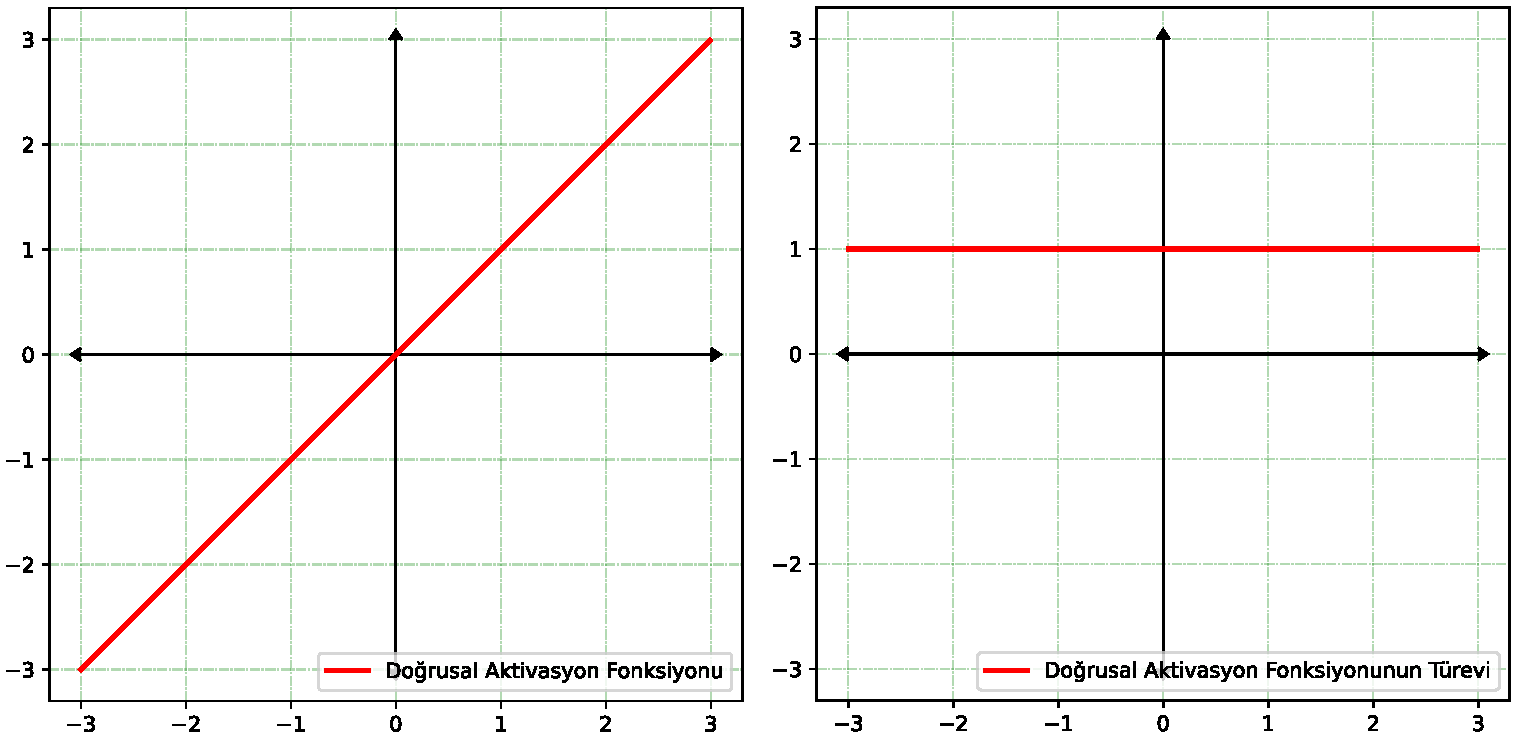
\includegraphics[scale=0.5]{Yapilan-Calismalar/Figures/lineer_comb.pdf}
    		}
    	\end{center}
    \end{figure}    
    Bu fonksiyonun türevinin sabit olması geri yayılım tekniği ile eğitim aşamasında çıkış ile giriş arasında bir ilişki kurulmasını mümkün kılmamaktadır. Ayrıca doğrusal aktivasyon fonksiyonu kullanıldığında doğrusal aktivasyon fonksiyonlarının kombinasyonları da doğrusal bir fonksiyon olduğundan katman sayısının da önemi ortadan kalkmaktadır. Bu durumda doğrusal aktivasyon fonksiyonları ile kurulan ardışıl katmanlar sanki tek bir katmanmış gibi davranmaktadırlar. Doğrusal aktivasyon fonksiyonu doğrusal kestirim modelleri kurmak için tercih edilen bir aktivasyon fonksiyonudur.
    
    \item Sigmoid Aktivasyon Fonksiyonu:
    
    Sigmoid aktivasyon fonksiyonu en tercih edilen aktivasyon fonksiyonlarından biridir. Türevinin kolay hesaplanabilir olması, monoton bir fonksiyon olması, yumuşak bir türevleme sunması gibi avantajları mevcuttur. Sigmoid aktivasyon fonksiyonu Eşitlik \ref{eq:sigmoid}, sigmoid aktivasyon fonksiyonunun türevi ise  Eşitlik \ref{eq:dsigmoid} kullanılarak hesaplanmaktadır.
    {\setlength{\mathindent}{0cm}
    \begin{equation}
    	\label{eq:sigmoid}
    	f(x)=O = \frac{1}{1+e^{-x}}
    \end{equation}
    \vspace{-1cm}
    \begin{equation}
    	\label{eq:dsigmoid}
    	f^{\prime}(x)= \frac{\partial L}{\partial  O}=O(1-O)
    \end{equation}}   
    Sigmoid aktivasyon fonksiyonu ve sigmoid aktivasyon fonksiyonunun türevi Şekil \ref{fig:sigmoid_comb}'de gösterilmektedir. Sigmoid aktivasyon fonksiyonu $[0 - 1]$ aralığında değer üretmektedir. Giriş $x$ değeri büyüdükçe yada küçüldükçe ani bir şekilde $0$ yada $1$'e yakınsadığı için sonucun net üretilebilmesini sağlamaktadır.
    
    \captionsetup[figure]{margin={0.3cm,-1cm}}
    \begin{figure}[h!]
    	\begin{center}
    		\vspace{0.4cm}
    		\captionbox{Sigmoid aktivasyon fonksiyonu ve türevi.\label{fig:sigmoid_comb}}
    		{
    			\vspace{0.4cm}
    			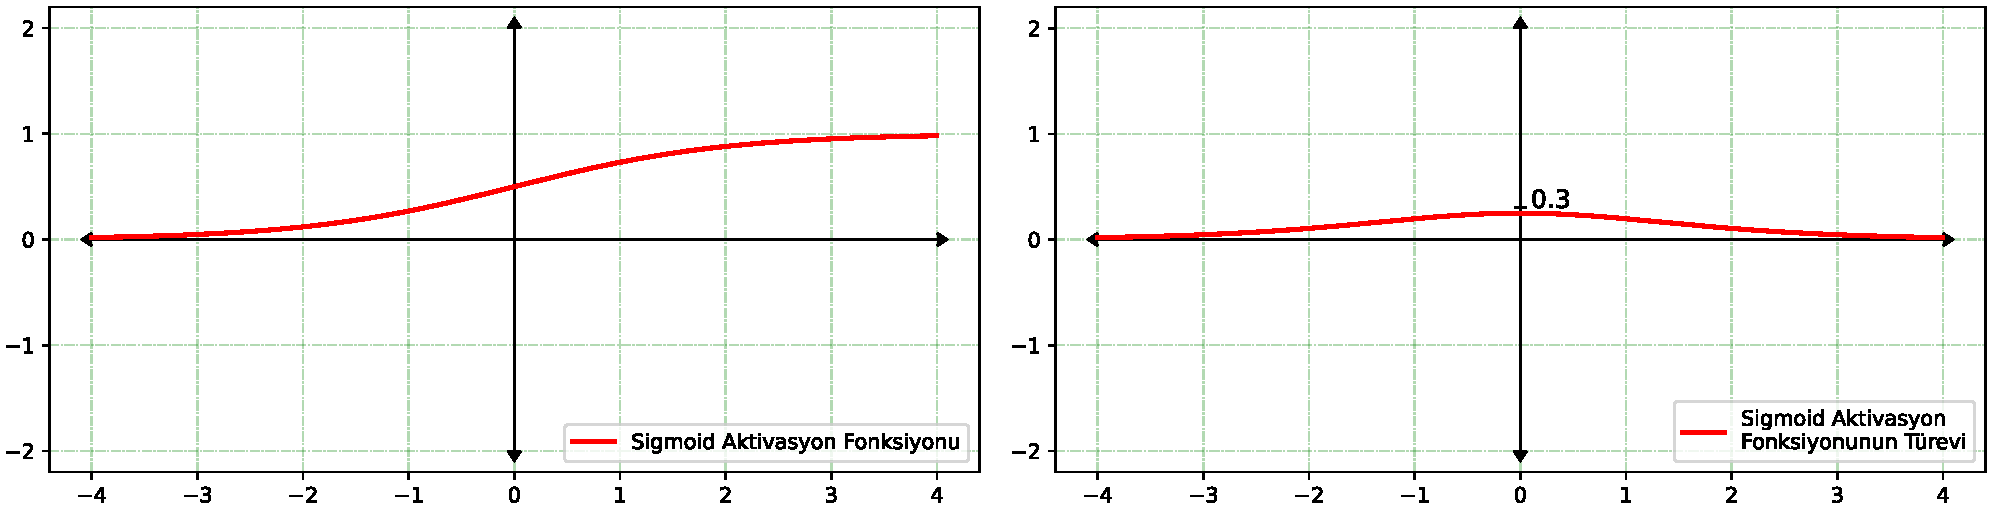
\includegraphics[scale=0.45]{Yapilan-Calismalar/Figures/sigmoid_comb.pdf}
    		}
    	\end{center}
    \end{figure}
    
    Katman sayısı arttıkça eğitim aşamasında sıfıra çok yakın türevler elde edilmekte ve dolayısıyla Kaybolan Eğim (Vanishing Gradient) problemi ile karşılaşılmaktadır \cite{hochreiter1998vanishing}. Tahmin merkezi sıfırın üzerinde olmaması ve katman sayısı arttıkça hesaplama maliyetinin artması sigmoid aktivasyon fonksiyonunun popülerliğini düşürmektedir. Genellikle çıkış katman aktivasyon fonksiyonu olarak tercih edilmektedir. Çıkış katmanı olarak Sigmoid aktivasyon fonksiyonu tercih edildiğinde eğitim veri seti $[0-1]$ aralığına uygun şekilde hazırlanmalıdır.
    
    \item Hiperbolik Tanjant Aktivasyon Fonksiyonu:
    
    Sigmoid aktivasyon fonksiyonuna oldukça benzer bir aktivasyon fonksiyonudur. Sigmoid aktivasyon fonksiyonundan en temel farklılığı $[-1,+1]$ aralığında değer üretmesinden dolayı sıfır merkezcil bir aktivasyon fonksiyonu oluşudur. Ayrıca sigmoid aktivasyon fonksiyonuna göre hiperbolik tanjant aktivasyon fonksiyonunun türevi Şekil \ref{fig:tanh_comb}'de gösterildiği gibi daha geniş aralıkta değerler alabilmektedir. Hiperbolik tanjant aktivasyon fonksiyonu Eşitlik \ref{eq:tanh}'de, hiperbolik tanjant aktivasyon fonksiyonunun türevi ise  Eşitlik \ref{eq:dtanh}'da verildiği gibi hesaplanmaktadır.
    {\setlength{\mathindent}{0cm}
    \begin{equation}
    	\label{eq:tanh}
    	f(x)=O=\frac{(e^{x} - e^{-x})}{(e^{x} - e^{-x})}
    \end{equation}
    \vspace{-1cm}
    \begin{equation}
    	\label{eq:dtanh}
    	f^{\prime}(x)= \frac{\partial L}{\partial  O} =1-O^{2}
    \end{equation}}    
    \captionsetup[figure]{margin={0.3cm,-1cm}}
    \begin{figure}[h!]
    	\begin{center}
    		\vspace{-0.6cm}
    		\captionbox{Hiperbolik tanjant aktivasyon fonksiyonu ve türevi.\label{fig:tanh_comb}}
    		{
    			\vspace{0.4cm}
    			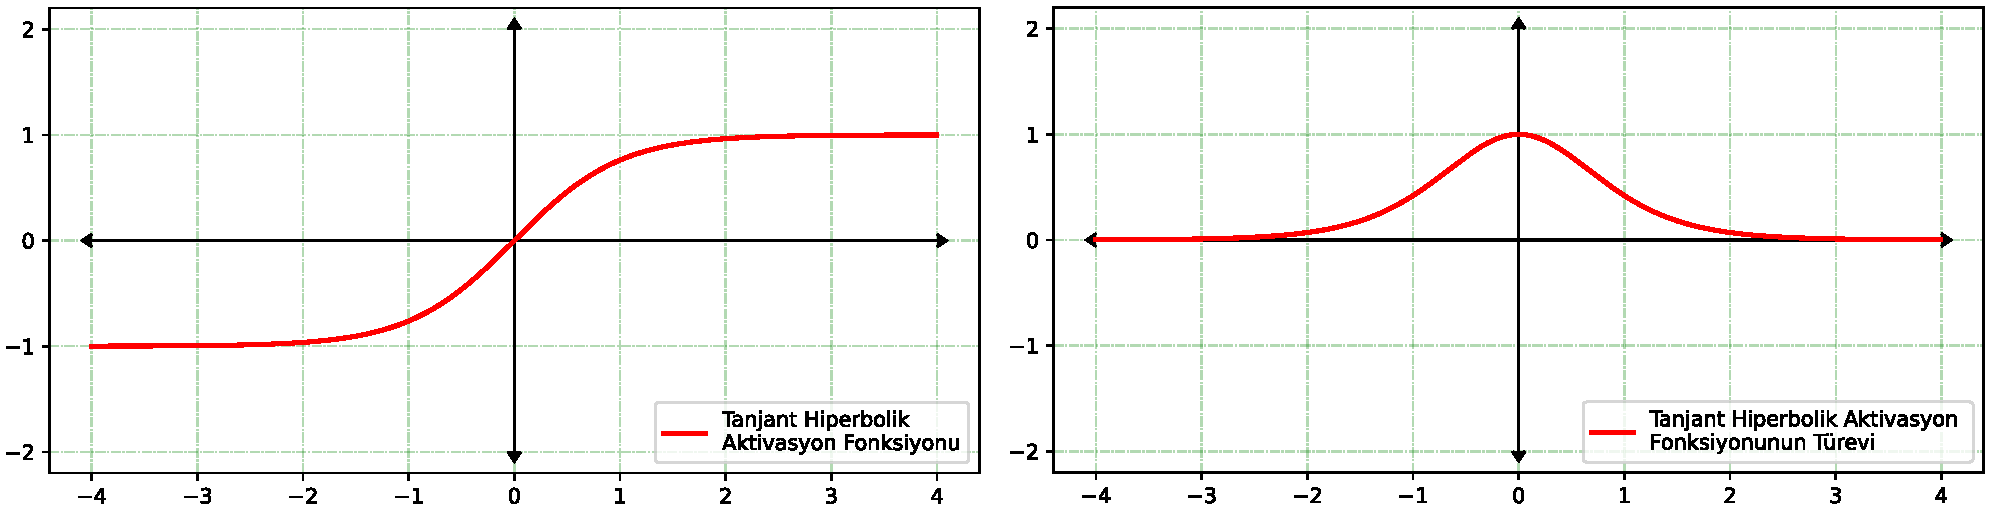
\includegraphics[scale=0.45]{Yapilan-Calismalar/Figures/tanh_comb.pdf}
    		}
    	\end{center}
    \end{figure}  
    
    \vspace{-0.6cm}
    Hiperbolik tanjant aktivasyon fonksiyonu, sigmoid aktivasyon fonksiyonunda olduğu gibi kaybolan eğim ve hesaplama maliyetinin yüksek olması gibi dezavantajlara sahiptir. Bu sebeplerden dolayı genellikle son katman aktivasyon fonksiyonu olarak tercih edilmektedir.
    
    \item ReLU Benzeri Aktivasyon Fonksiyonları:
    
    Doğrultulmuş Doğrusal Birim (Rectified Linear Unit - ReLU) aktivasyon fonksiyonu çok katmanlı mimarilerde kaybolan eğim (vanishing gradient) problemine çözüm olarak kullanılmaya başlanan bir aktivasyon fonksiyonudur \cite{hochreiter1998vanishing}. ReLU aktivasyon fonksiyonu Eşitlik \ref{eq:relu}, ReLU aktivasyon fonksiyonunun türevi ise  Eşitlik \ref{eq:drelu} kullanılarak hesaplanmaktadır.
    {\setlength{\mathindent}{0cm}
    \begin{equation}
    	\label{eq:relu}
    	f(x)= O = \left\{\begin{array}{ll}
    		0 & \text { for } x<0 \\
    		x & \text { for } x \geq 0
    	\end{array}\right.
    \end{equation}
    \vspace{-1cm}
    \begin{equation}
    	\label{eq:drelu}
    	f^{\prime}(x)= \frac{\partial L}{\partial  O} = \left\{\begin{array}{ll}
    		0 & \text { for } x<0 \\
    		1 & \text { for } x \geq 0
    	\end{array}\right.
    \end{equation}}    
    Şekil \ref{fig:relu_comb}'da gösterildiği gibi ReLU aktivasyon fonksiyonu $[0,+\infty]$ aralığında çıkış değeri üretebilmekte ve negatif değerler için $0$, pozitif değerler için $1$ türevini sağlamaktadır. ReLU aktivasyon fonksiyonu sigmoid ve hiperbolik tanjant aktivasyonunun aksine negatif eksende $0$ değerini üretmesinden ve ileri yönlü hesaplamada $0$ çıkışlı algılayıcıların tetiklenmemesinden dolayı çok daha düşük hesaplama maliyetine sahiptir. Doğrusal bir aktivasyon fonksiyonuna ne kadar benzese de aslında doğrusal olmayan bir aktivasyon fonksiyonudur. Bu fonksiyon farklı aktivasyon fonksiyonları ile birlikte birleştirilerek kullanılabilmektedir.
    
    \captionsetup[figure]{margin={0.3cm,-1cm}}
    \begin{figure}[h!]
    	\begin{center}
    		\vspace{0.4cm}
    		\captionbox{ReLU benzeri aktivasyon fonksiyonları ve bu  fonksiyonların türevleri.\label{fig:relu_comb}}
    		{
    			\vspace{0.4cm}
    			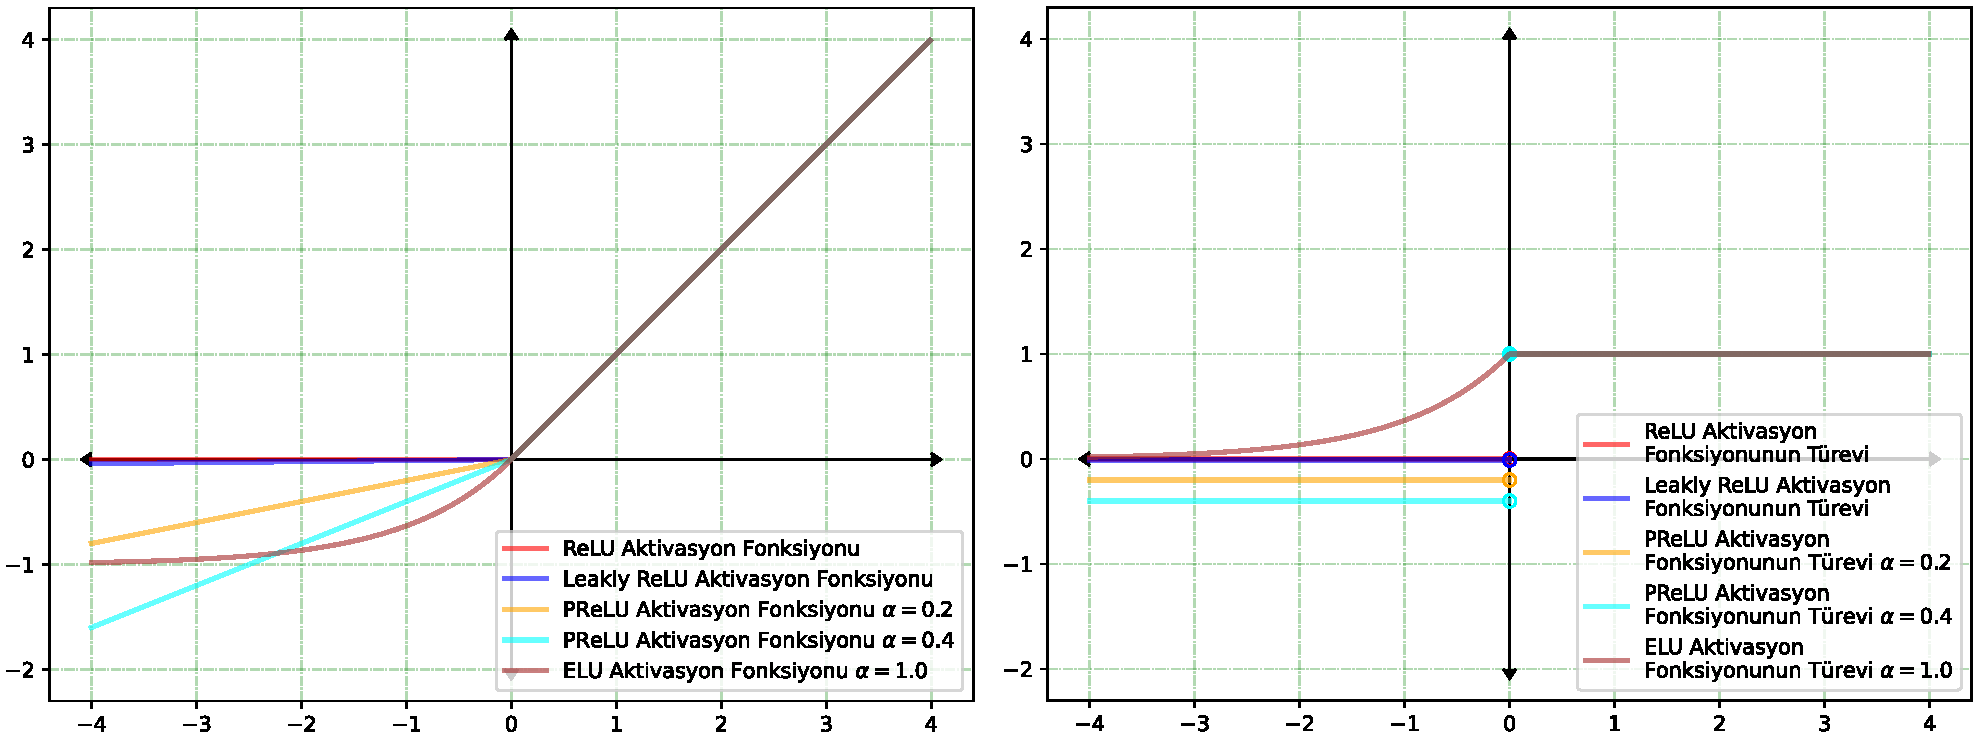
\includegraphics[scale=0.45]{Yapilan-Calismalar/Figures/relu_comb.pdf}
    		}
    	\end{center}
    \end{figure}
    
    ReLU aktivasyon fonksiyonu girişinden $0$ yada sıfırın altında değer geldiğinde sürekli $0$ çıkışını üretmektedir. Bu durum Ölen ReLU Problemi (The Dying ReLU Problem) adı verilen, eğitimin gerçekleşmediği katmanların ortaya çıkmasına sebebiyet vermektedir. Bundan dolayı ReLU aktivasyon fonksiyonu güncellenerek Sızan ReLU (Leaky ReLU), Parametrik ReLU (Parametric ReLU - PReLU), Eksponansiyel Doğrusal Birim (Exponential Linear Unit - ELU) gibi aktivasyon fonksiyonları ortaya çıkarılmıştır.
    
    \begin{itemize}
    	\item Leaky ReLU aktivasyon fonksiyonu ReLU aktivasyon fonksiyonundan farklı olarak $0$'dan küçük değerler için de değerler üretilebilmesini sağlamaktadır. Leaky ReLU aktivasyon fonksiyonu Eşitlik \ref{eq:lrelu}, ReLU aktivasyon fonksiyonunun türevi ise  Eşitlik \ref{eq:dlrelu}'teki gibi hesaplanmaktadır. 
    	{\setlength{\mathindent}{-1cm}
    	\begin{equation}
    		\label{eq:lrelu}
    		f(x)= O = \left\{\begin{array}{ll}
    			0.01x & \text { for } x<0 \\
    			x & \text { for } x \geq 0
    		\end{array}\right.
    	\end{equation}
    	\vspace{-1cm}
    	\begin{equation}
    		\label{eq:dlrelu}
    		f^{\prime}(x)= \frac{\partial L}{\partial  O} =\left\{\begin{array}{ll}
    			0.01 & \text { for } x<0 \\
    			1 & \text { for } x \geq 0
    		\end{array}\right.
    	\end{equation}}
    	\item PReLU aktivasyon fonksiyonu Leaky ReLU aktivasyon fonksiyonunun geliştirilmiş versiyonudur. Leaky ReLU aktivasyon fonksiyonunda $0$'dan küçük değerler $0.01$ sabit katsayısı ile çarpılırken, PReLU aktivasyon fonksiyonunda bu değerin $\alpha$ parametresi ile değiştirilebilir olması sağlanmaktadır. PReLU aktivasyon fonksiyonu Eşitlik \ref{eq:prelu}, ReLU aktivasyon fonksiyonunun türevi ise Eşitlik \ref{eq:dprelu}'te verildiği gibi hesaplanmaktadır.
    	{\setlength{\mathindent}{-1cm}
    	\begin{equation}
    		\label{eq:prelu}
    		f(x)= O =\left\{\begin{array}{ll}
    			\alpha x & \text { for } x<0 \\
    			x & \text { for } x \geq 0
    		\end{array}\right.
    	\end{equation}
    	\vspace{-1cm}
    	\begin{equation}
    		\label{eq:dprelu}
    		f^{\prime}(x)= \frac{\partial L}{\partial  O} = \left\{\begin{array}{ll}
    			\alpha & \text { for } x<0 \\
    			1 & \text { for } x \geq 0
    		\end{array}\right.
    	\end{equation}}
    	\item ELU aktivasyon fonksiyonu $0$'dan küçük değerler için $\alpha$ parametre değerine göre doğrusal olmayan değerler üretilebilmesini sağlamaktadır. ELU aktivasyon fonksiyonu Eşitlik \ref{eq:elu}, ReLU aktivasyon fonksiyonunun türevi ise Eşitlik \ref{eq:delu}'de gösterildiği gibi hesaplanmaktadır.
    	{\setlength{\mathindent}{-1cm}
    	\begin{equation}
    		\label{eq:elu}
    		f(x)= O = \left\{\begin{array}{ll}
    			\alpha(e^{x}-1) & \text { for } x<0 \\
    			x & \text { for } x \geq 0
    		\end{array}\right.
    	\end{equation}
    	\vspace{-1cm}
    	\begin{equation}
    		\label{eq:delu}
    		f^{\prime}(x)= \frac{\partial L}{\partial  O} =\left\{\begin{array}{ll}
    			\alpha e^{x} & \text { for } x<0 \\
    			O+\alpha & \text { for } x \geq 0
    		\end{array}\right.
    	\end{equation}}
    \end{itemize}
    
    \item Softmax Aktivasyon Fonksiyonu:
    
    Çok sınıflı sınıflandırma ihtiyacı doğrultusunda ortaya çıkarılmış bir aktivasyon fonksiyonudur. Softmax aktivasyon fonksiyonu haricindeki diğer tüm aktivasyon fonksiyonları iki sınıflı sınıflandırma aktivasyon fonksiyonlarıdır. Bu aktivasyon fonksiyonunun çıkış katmanındaki herbir algılayıcı çıkışı için sınıf sayısı uzunluğunda vektör oluşturulmaktadır. İleri yönde hesaplamada bu vektörün maksimum değerli indisleri girişten gelen verinin hangi sınıfa dahil olduğunu göstermektedir. Bu vektörün uzunluğu $n$ olarak kabul edilirse, $i$ inci indeksteki çıkış değeri $i$ sınıfı temsil etmek üzere Eşitlik \ref{eq:softmax}'deki gibi hesaplanmaktadır. Softmax fonksiyonunun türevi hesaplanırken, aslında tüm birinci dereceden kısmi türevlerin matrisi olan Jacobian matrisinin hesaplanması gerekmektedir. Eşitlik \ref{eq:dsoftmax}'da softmax aktivasyon fonksiyonunun türevi gösterilmektedir.
    {\setlength{\mathindent}{0cm}
    \begin{equation}
    	\label{eq:softmax}
    	f_{i}(\vec{x})= O_{i} =\frac{e^{x_{i}}}{\sum_{j=1}^{n} e^{x_{j}}} \quad \text { , } \quad \forall i=1, \ldots, n
    \end{equation}
    \vspace{-1cm}
    \begin{equation}
    	\label{eq:dsoftmax}
    	f^{\prime}_{i}(\vec{x})= \frac{\partial L}{\partial  O_{i}} = O_{i}(1\left\{i=j\right\}-O_{j}) \quad \text { , } \quad \forall i=1, \ldots, n \quad \text { , } \quad \forall j=1, \ldots, n
    \end{equation}}
    Softmax aktivasyon fonksiyonu sadece çıkış katmanında tercih edilen bir aktivasyon fonksiyonudur. 
\end{itemize}

\subsubsection{Yukarı Örnekleme Katmanları}
Yukarı örnekleme (Up Sampling) katmanları ters konvolüsyon katmanları gibi boyut artırma işlemi için tercih edilebilecek katmanlardandır. Yukarı örnekleme katmanları girişten uygulanan $G$ özellik haritasına interpolasyon teknikleri uygulayarak daha büyük ebatlarda çıkış $O$ özellik haritaları elde edilmesini sağlamaktadır. Yukarı örnekleme katmanlarında ters konvolüsyon katmanlarının aksine eğitilebilir parametre bulunmamaktadır. Bu sebeple yukarı örnekleme katmanları ardından dolgulama gerçekleştirilmiş konvolüsyon katmanları eklenerek eğitilebilir bloklar üretilebilmektedir \cite{dumoulin2016guide}. Yukarı örnekleme katmanları ardından konvolüsyon katmanları kullanılmaması durumunda eğitim olumsuz etkilenmektedir.

\subsubsection{Havuzlama Katmanları}
Havuzlama katmanı eğitilebilir parametresi bulunmayan katmanlardandır. Genellikle hesaplama maliyetini düşürmek ve konvolüsyon katmanlarından sonra boyut azaltma işlemi için tercih edilmektedirler. Bir anlamda konvolüsyon katmanlarından elde edilen özellik haritalarının özetlenmesi işlemini gerçekleştirmektedirler. Böylece çıkarılan özellikler konumsal değişimlere daha dayanıklı hale getirilmiş olmaktadırlar. Havuzlama uygulanacak özellik haritasının havuzlama bölgesi $P$ ve $P$'nin alt havuzlama bölgesi $E$ Eşitlik \ref{eq:pooling1}'da gösterildiği gibi temsil edilmektedir.
\begin{equation}
	\label{eq:pooling1}
	E_{P} = \left\{ e_{k} \mid k \in P \right\}
\end{equation}
    
Literatürde birçok havuzlama tekniği olmakla birlikte genellikle maksimum havuzlama ve ortalama havuzlama yöntemleri tercih edilmektedir. Maksimum havuzlamada $P$ havuzlama bölgesinin $E_{P}$ alt havuzlama bölgesinde Eşitlik \ref{eq:maxpooling}'deki gibi maksimum değerli değeri seçilirken, ortalama havuzlamada $E_{P}$ alt bölgesinin Eşitlik \ref{eq:meanpooling}'deki gibi değerlerinin ortalaması hesaplanarak bu ortalama değerleri kullanılmaktadır.
\begin{equation}
	\label{eq:maxpooling}
	P_{maksimum} = maksimum(E_{P})
\end{equation}
\vspace{-1cm}
\begin{equation}
	\label{eq:meanpooling}
	P_{ortalama} = \frac{\sum E_{P}}{\left| E_{P} \right|}
\end{equation}

\captionsetup[figure]{margin={0.3cm,-3.2cm}}
\begin{figure}[h!]
	\begin{center}
		\vspace{0.4cm}
		\captionbox{Maksimum ve Ortalama havuzlama tekniklerinin $4 \times 4$ boyutuna sahip özellik haritasına uygulanması.\label{fig:pooling}}
		{
			\vspace{0.4cm}
			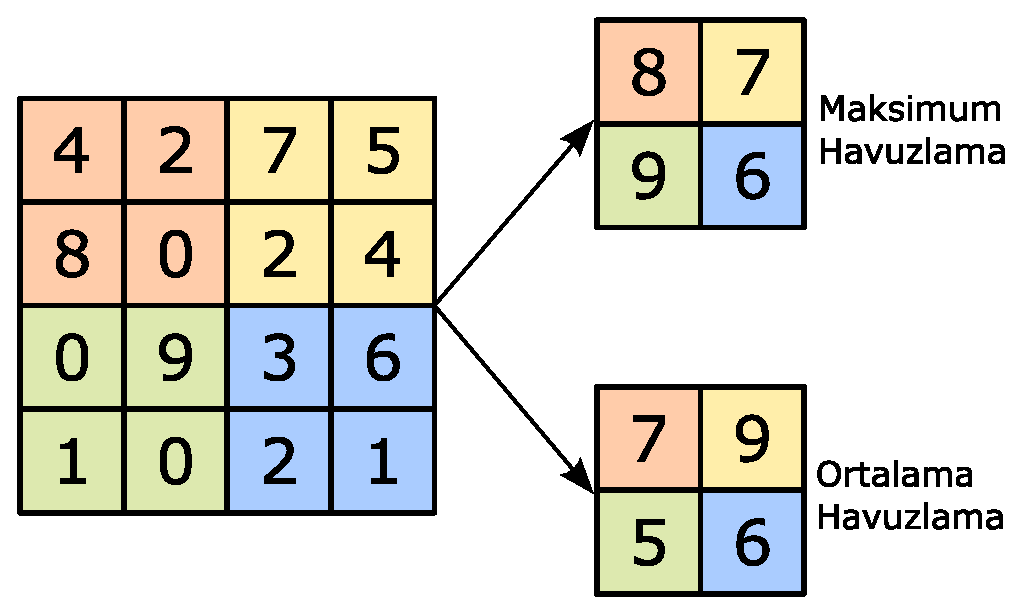
\includegraphics[scale=0.5]{Yapilan-Calismalar/Figures/pooling.pdf}
		}
	\end{center}
\end{figure}

Maksimum ve ortalama havuzlama tekniklerinde havuzlama miktarı $p=2 \times 2$, adım kaydırma miktarı $s=2$ seçildiğinde, bu havuzlama tekniklerinin $4 \times 4$ boyutuna sahip özellik haritasına uygulanması Şekil \ref{fig:pooling}'de gösterildiği gibi olmaktadır.

Havuzlama katmanı girişine uygulanan $G$ özellik haritasının havuzlama işlemi sonrası elde edilen çıkış özellik haritasının $O$ ebatları Eşitlik \ref{eq:poolingsize}'teki gibi hesaplanabilmektedir. 
\begin{equation}
	\label{eq:poolingsize}
	O=\left\lfloor \frac{G-p}{s} \right\rfloor+1
\end{equation}

\subsubsection{Birleştirme Katmanları}
Birleştirme katmanı, iki farklı katmanın çıkışı olan özellik haritalarının birleştirilmesinde kullanılmaktadır. İki farklı katmanın çıkışı olan özellik haritalarının birleştirilebilmesi için özellik haritalarının ebatlarının aynı olması gerekmektedir. Birleştirilecek özellik haritası sayısının farklı ve aynı sayıda olması durumları için iki farklı birleştirme yöntemi mevcuttur.

\captionsetup[figure]{margin={0.4cm,-1cm}}
\begin{figure}[h!]
	\begin{center}
		\vspace{0.4cm}
		\captionbox{Derinlik birleştirme işlemi (Concatenate).\label{fig:concatenate}}
		{
			\vspace{0.4cm}
			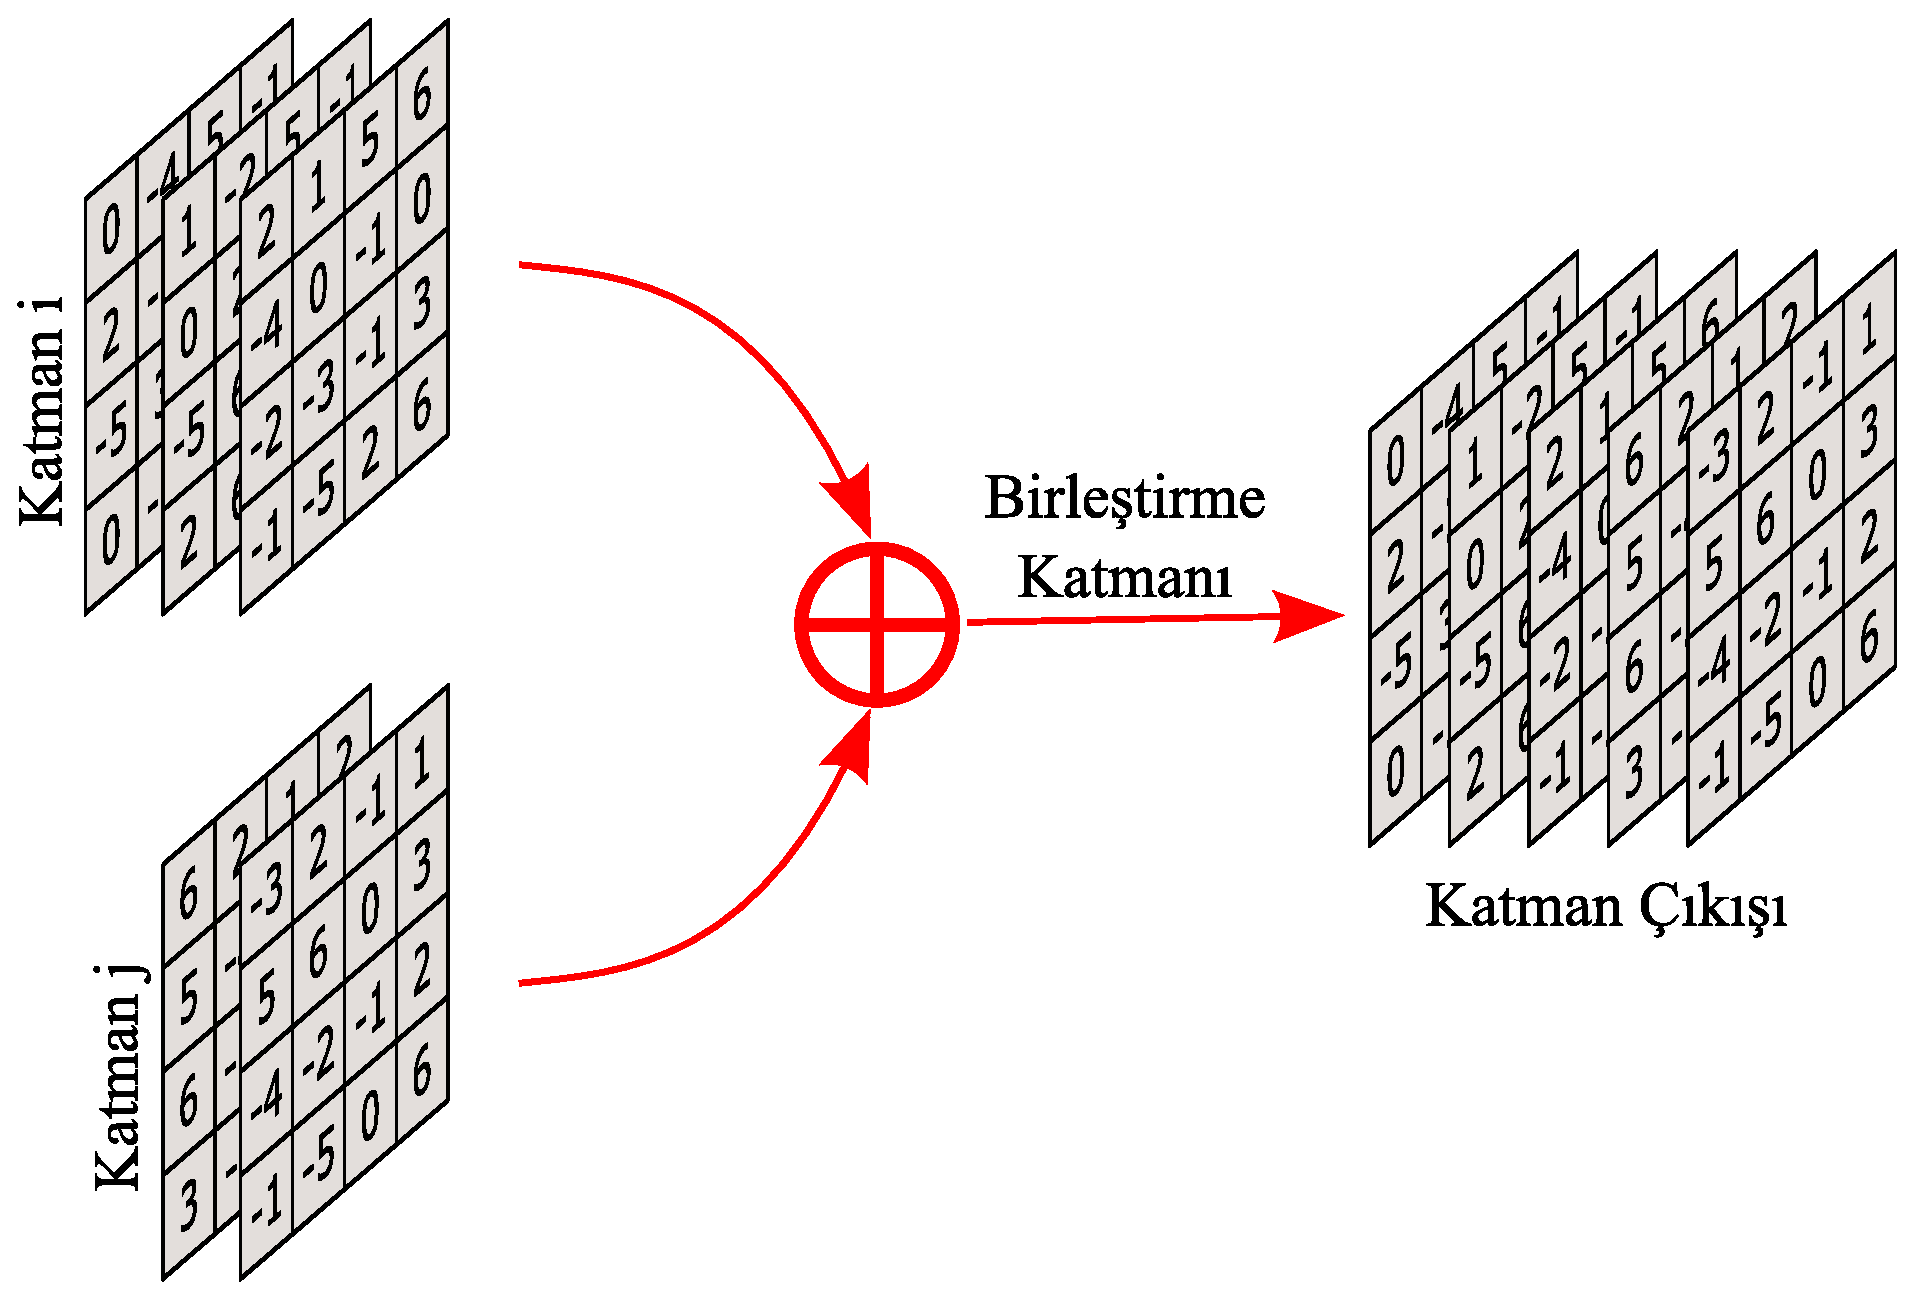
\includegraphics[scale=0.43]{Yapilan-Calismalar/Figures/concatenate.pdf}
		}
	\end{center}
\end{figure}

İki farklı katmanın özellik haritası sayılarının farklı olması durumunda derinlik birleştirme işlemi gerçekleştirilebilmektedir. Derinlik birleştirme katmanında iki farklı katman çıkışındaki özellik haritaları Şekil \ref{fig:concatenate}'de gösterildiği gibi birleştirilmektedir. Derinlik birleştirme katmanları genellikle oto-kodlayıcılarda karşımıza çıkmaktadır. Çok tercih edilen U-Net oto kodlayıcılarılarında \cite{ronneberger2015u} atlama bağlantıları ile konvolüsyon ve ters konvolüsyon katmanlarının çıktıları derinlik birleştirme işlemi ile birleştirilmektedir.

İki farklı katmanın özellik haritalarının aynı sayıda olması durumunda ise derinlik birleştirme işlemi gerçekleştirilebildiği gibi ekleme işlemi de gerçekleştirilebilmektedir. Ekleme katmanı iki katmandaki aynı indisli özellik haritalarını birleştirerek Şekil \ref{fig:add}'de gösterildiği gibi aynı sayıda özellik haritası üretmektedir. Özellik haritaları için ekleme işlemi literatürde ilk kez ResNet mimarisinde \cite{he2016deep} rastlanmaktadır. Derin ağlarda ilk katmanlardaki özellik haritalarında bulunan bilgiler katman sayısı arttıkça kaybolmaya başlamaktadır. Bu sebeple ekleme katmanı kullanılarak önceki katmanlardaki bilgi ileri katmanlarla birleştirilmekte ve böylece önemli bilgi kaybının önüne geçilebilmektedir.

\captionsetup[figure]{margin={0.3cm,-1cm}}
\begin{figure}[h!]
	\begin{center}
		\vspace{0.4cm}
		\captionbox{Derinlik ekleme işlemi (Add).\label{fig:add}}
		{
			\vspace{0.4cm}
			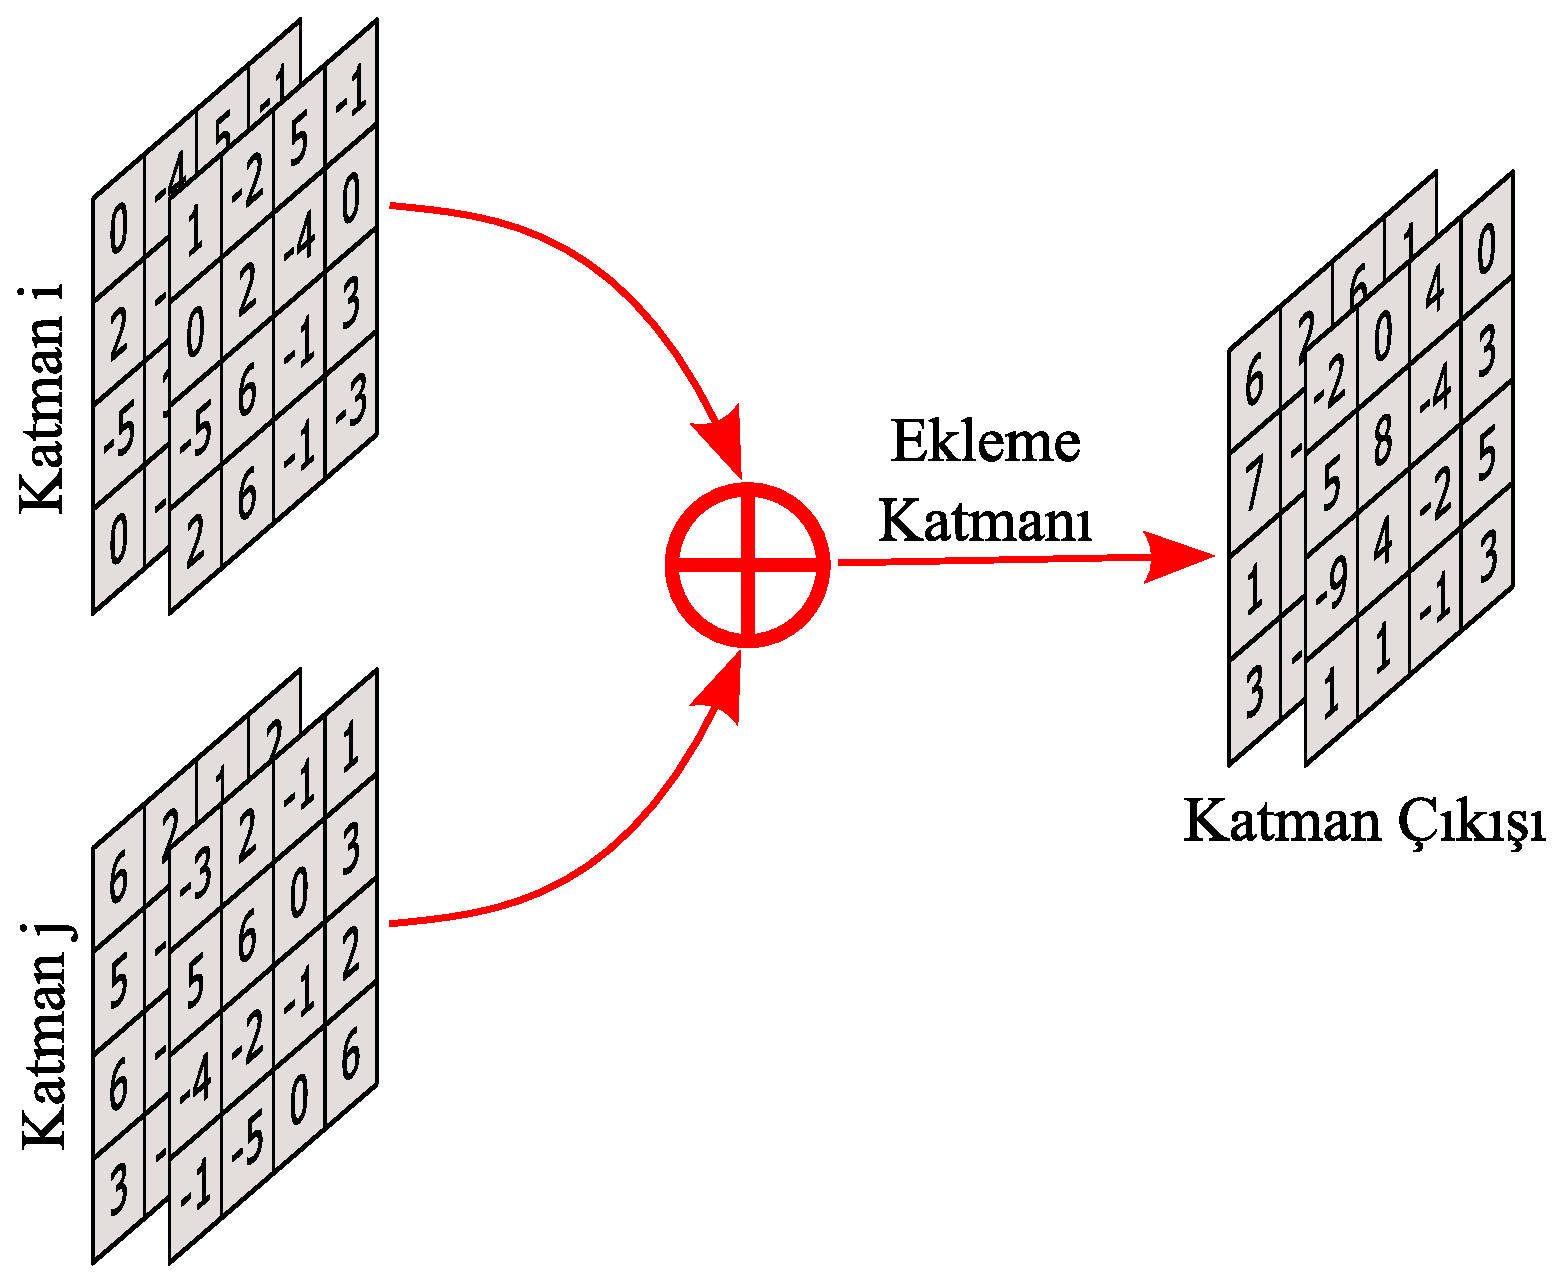
\includegraphics[scale=0.43]{Yapilan-Calismalar/Figures/add.pdf}
		}
	\end{center}
\end{figure}

\subsubsection{Düzleştirme Katmanları}
Düzleştirme (Flatten) katmanları girişinden $n$ boyutlu veri alıp çıkışından $n$ boyutlu veri üretebilen konvolüsyon gibi katmanların çıkışının sınıflandırma katmanlarına uydurulmasında kullanılan katmanlardır. Tam bağlantılı katmanlar giriş verisi olarak bir boyutlu $x$ vektörlerini kabul etmektedirler. Bu sebeple konvolüsyon katmanı gibi $n$ boyutlu çıkış üretebilen katmanların çıkışlarının sınıflandırıcı katmanlara aktarılmadan önce düzleştirilmesi gerekmektedir. Düzleştirme katmanlarının eğitilebilir parametresi bulunmamaktadır. Şekil \ref{fig:flattening}'te gösterildiği gibi düzleştirme katmanı girişinden uygulanan $n$ boyutlu veriyi bir boyutlu vektöre dönüştürmektedir. Düzleştirme katmanı girişinden birden çok özellik haritası uygulandığında birleştirme katmanlarında olduğu gibi verileri birleştirip bir boyutlu tek bir vektöre dönüştürmektedir.

\captionsetup[figure]{margin={0.3cm,-2cm}}
\begin{figure}[h!]
	\begin{center}
		\vspace{0.4cm}
		\captionbox{2B özellik haritasının düzleştirilmesi. \label{fig:flattening}}
		{
			\vspace{0.4cm}
			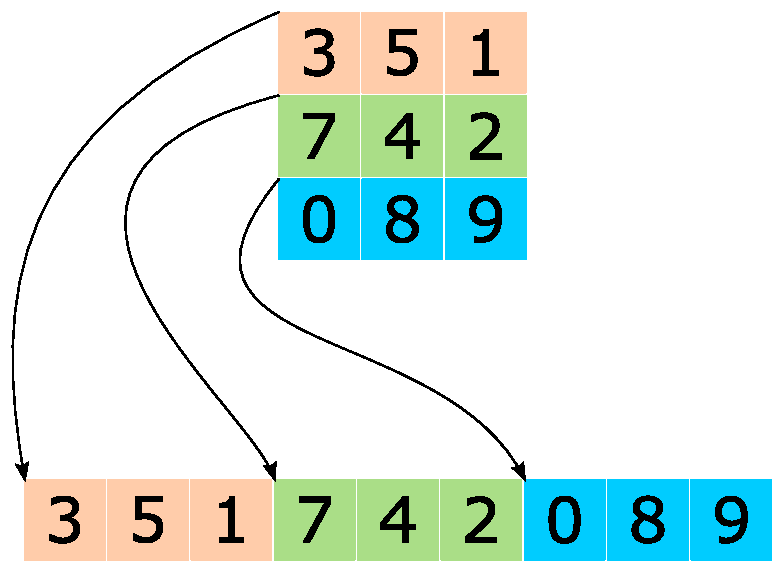
\includegraphics[scale=0.6]{Yapilan-Calismalar/Figures/flattening.pdf}
		}
	\end{center}
\end{figure}

\subsubsection{Seyreltme Katmanları \label{lyr:dropout}}
Seyreltme katmanları aslında bir düzenleştirme katmanıdır. Tam bağlantılı katmanlardan sonra kullanılarak ağın aşırı öğrenme (over fitting) problemi ile karşılaşmasını engelleme fikri ile ortaya atılmıştır \cite{srivastava2014dropout}. Kendisinden önce gelen tam bağlantılı katmandaki belirtilen oranda sinir hücresini rasgele olarak kapatarak eğitim aşamasında eğitim verisinin sürekli aynı yollar üzerinden akmasını engellemektedir. Bu katman sinir hücresi ağırlıklarının dengeli bir şekilde eğitilmesini sağlamaktadır. Rasgele sinir hücrelerinin kapatılmasındaki amaç tam bağlantılı katmanın herhangi bir sinir hücresine bağımlılığının azalmasıdır. Birlikte çalışan fazla sayıda sinir hücresi, modelin daha karmaşık işlevleri öğrenmesine de sebep verebildiği için seyreltme katmanlarının kullanılması modelin eğitim verilerindeki gürültü ve diğer bozulmalara daha dayanıklı olmasını sağlamaktadır.

Seyreltme katmanlarında kapatılan sinir hücreleri modelden çıkarılmış olmamaktadır. Sadece kapatılan sinir hücrelerinin çıkışları sıfırlanmaktadır. Bu sebeple modeldeki sinir hücresi sayısı değişmediğinden bu katmanın eğitim süresi üzerine hızlandırma etkisi bulunmamaktadır.

\captionsetup[figure]{margin={0.3cm,0cm}}
\begin{figure}[h!]
	\begin{center}
		\vspace{0.4cm}
		\captionbox{Tam bağlantılı katmana 0.5 oranında seyreltme gerçekleştiren seyreltme katmanı.\label{fig:dropout}}
		{
			\vspace{0.4cm}
			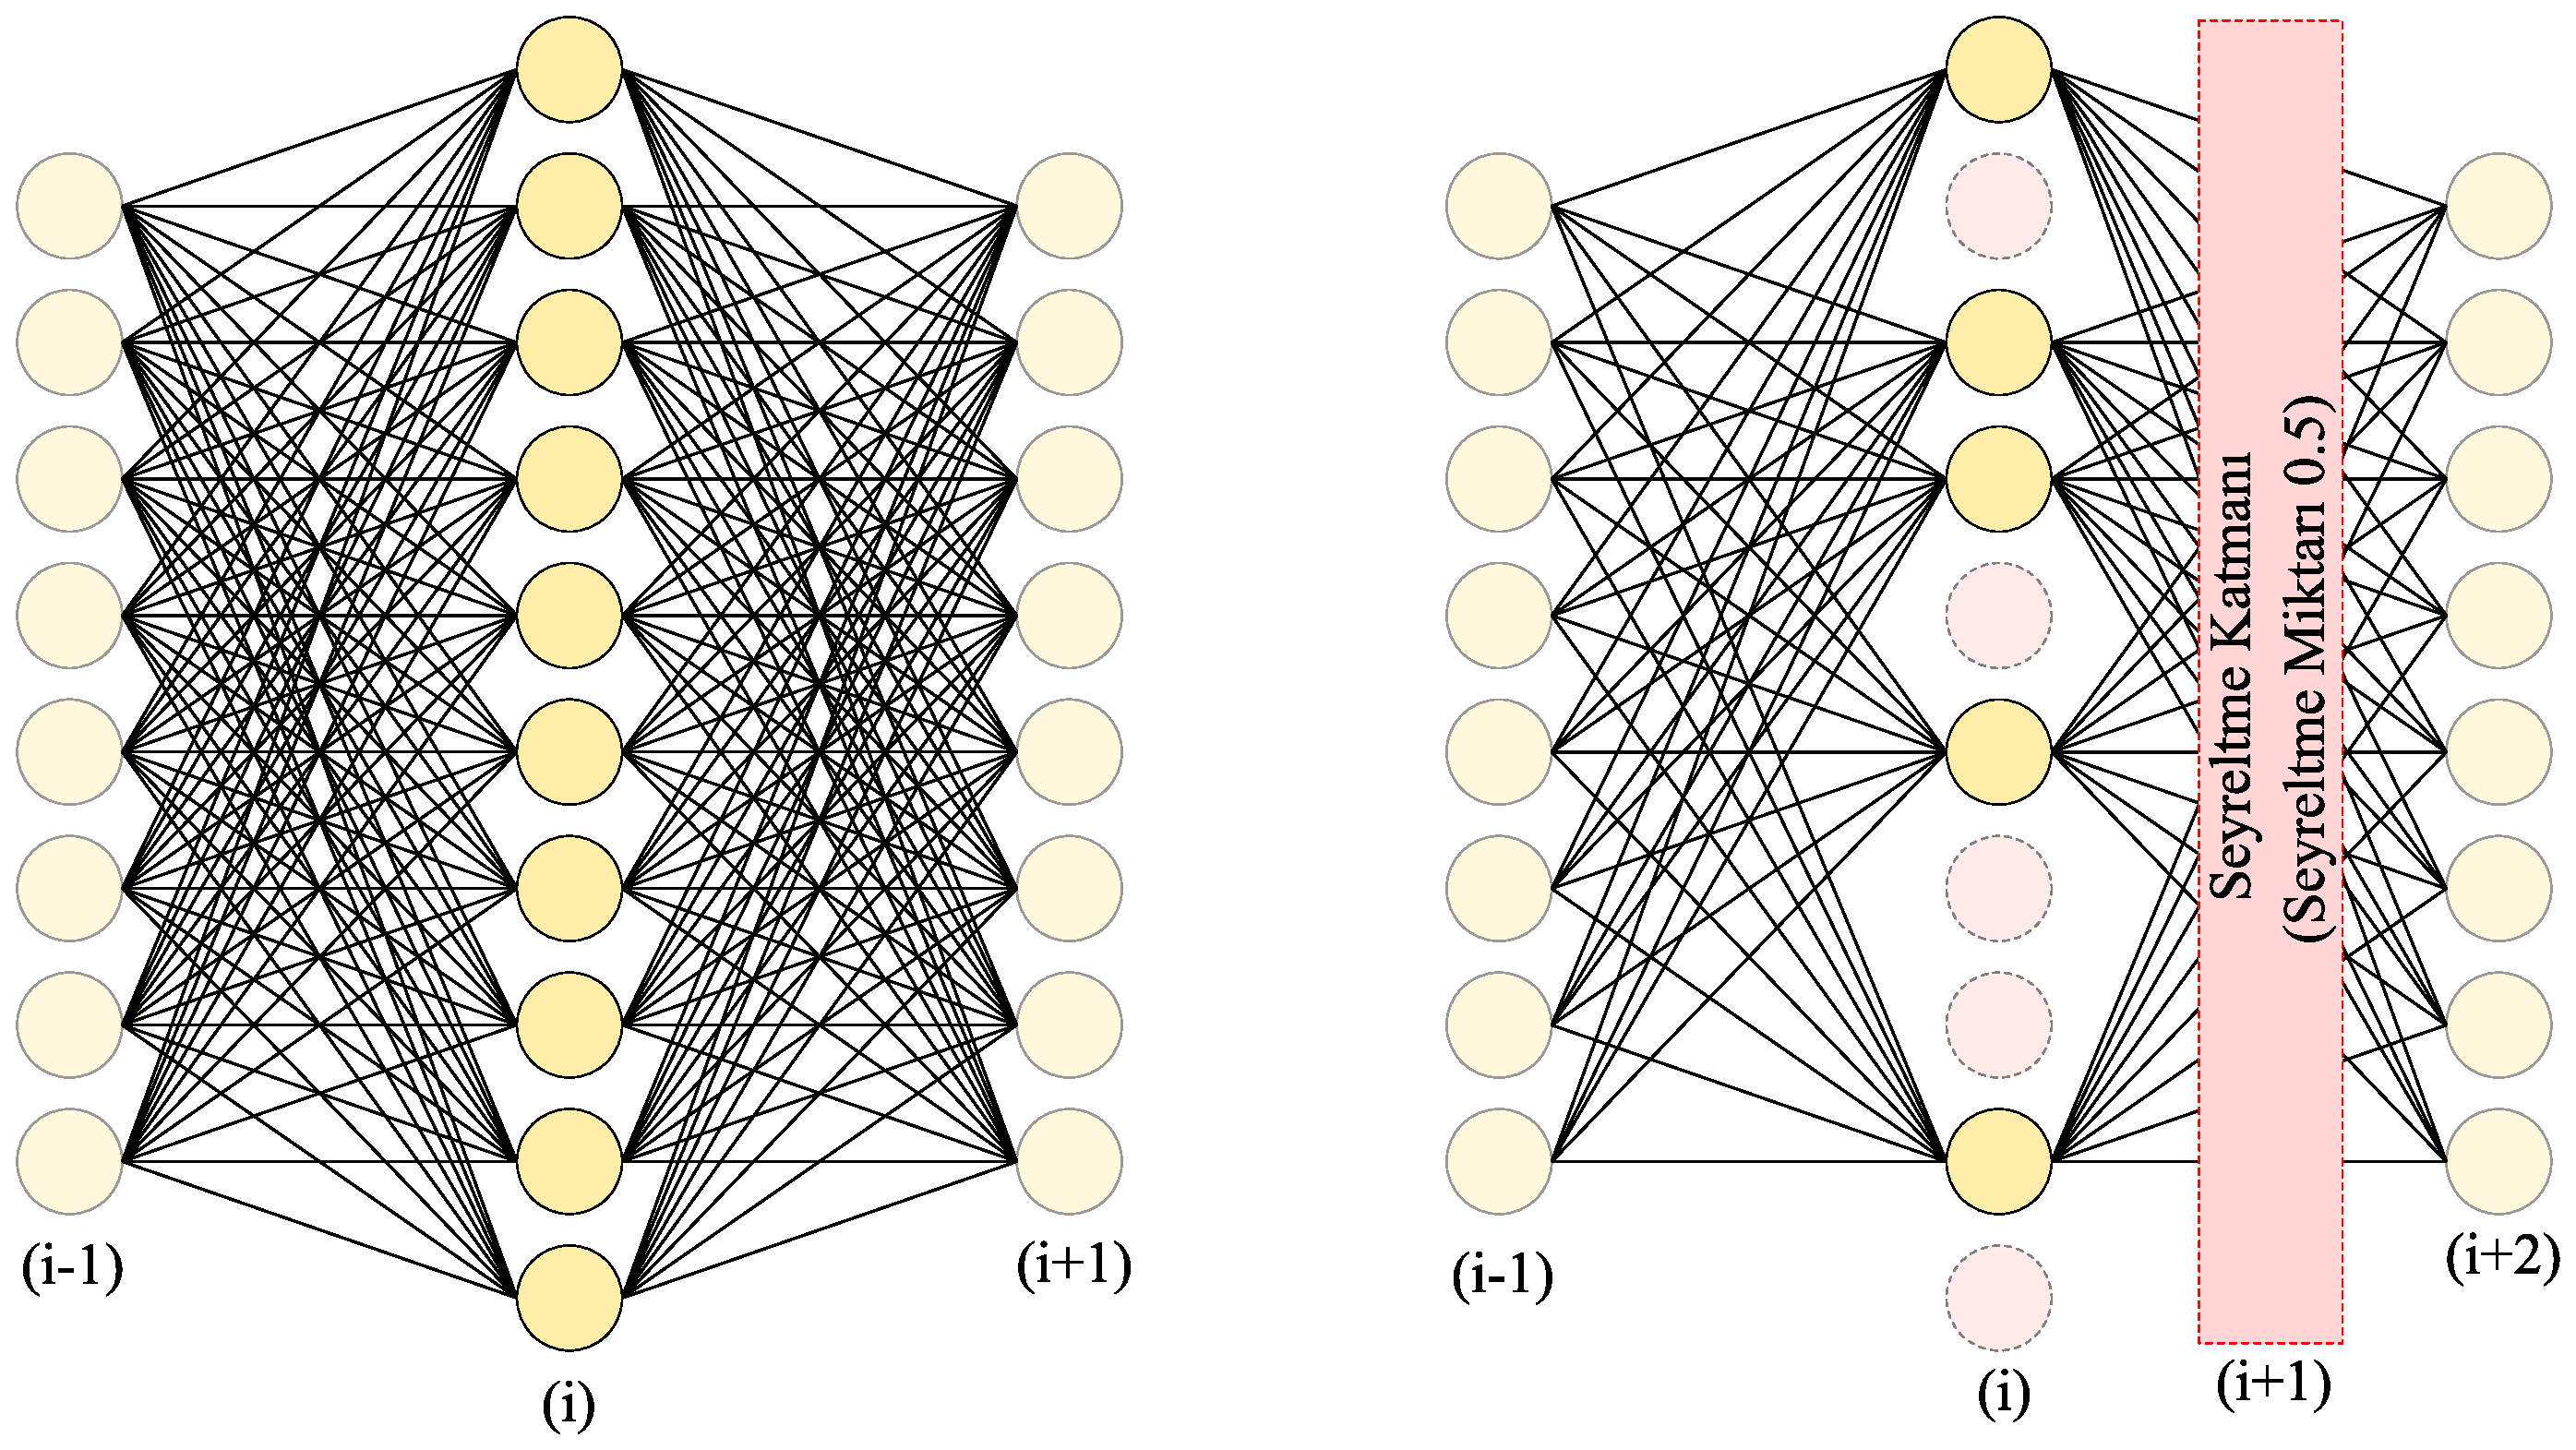
\includegraphics[scale=0.32]{Yapilan-Calismalar/Figures/dropout.pdf}
		}
	\end{center}
\end{figure}

Seyreltme katmanlarında rastgeleliği artırmak için genellikle Bernoulli dağılımı tercih edilmektedir. Bernoulli dağılımı, $p$ olasılığı ile $1$ değerinin ve $q$ olasılığı ile $0$ değerinin elde edilebildiği ikili (ayrık) bir olasılık dağılımıdır. Rasgele seçilmiş $r_{i}$ değerlerinden $r_{i}=1$ için Eşitlik \ref{eq:bernouli1}, $r_{i}=0$ için Eşitlik \ref{eq:bernouli0}'teki gibi bir olasılık söz konusu olmaktadır. Şekil \ref{fig:dropout}'te tam bağlantılı katmana 0.5 oranında seyreltme gerçekleştiren seyreltme katmanı gösterilmektedir.
\begin{equation}
	\label{eq:bernouli1}
	P(r_{i}=1) = p
\end{equation}
\vspace{-1cm}
\begin{equation}
	\label{eq:bernouli0}
	P(r_{i}=0) = q = 1 - p = 1 - P(r_{i}=1)
\end{equation}

Eşitlik \ref{eq:bernouli1} ve \ref{eq:bernouli0}'in anlamı, seyreltme değerinin $1$ olma olasılığının $p$ olduğu, $0$ olma olasılığı $q = 1 - p$ olduğudur. Böylece Eşitlik \ref{eq:bernouli2} elde edilmektedir.
\begin{equation}
	\label{eq:bernouli2}
	r_{i} \sim \textit{Bernoulli}(p)
\end{equation}

Eşitlik \ref{eq:bernouli2}'nın anlamı $r_{i}$ değerinin Bernoulli dağılımı $1$ olan bir $p$ olasılık değerinin eşdeğeri olduğudur. Bu olasılık dağılımları ile değeri $1$ olan $p$ dağılımına sahip sinir hücrelerinin çıkışları $1$ ile çarpılarak çalışmaya devam etmesi, değeri 0 olan sinir hücrelerinin çıkışları 0 ile çarpılarak seyreltilmesi sağlanmaktadır. $r_{i}$ inci sinir hücresinin çıkışını $z_{i}$ ve seyreltme katmanını $Sr$ olarak kabul edersek seyreltme işlemi Eşitlik \ref{eq:seyreltme}'deki gibi hesaplanmaktadır.
\begin{equation}
	\label{eq:seyreltme}
	Sr_{i} =  \left\{ 
	\begin{array}{ c l }
		\frac{z_{i}}{1-q} & \quad r_{i} = 1 \\
		0                 & \quad r_{i} = 0 
	\end{array}
	\right.
\end{equation}

Eğitim aşamasında her katmanda olduğu gibi seyreltme katmanının ters yönde hesaplaması gerçekleştirilirken zincir kuralına göre türevlenmesi gerekmektedir. Bu sebeple $r_{i}$ inci sinir hücresinin $z_{i}$ çıkışının $Sr$ seyreltme katmanına göre kısmi türevi Eşitlik \ref{eq:seyreltmederiv}'de verildiği gibi hesaplanmaktadır.
\begin{equation}
	\label{eq:seyreltmederiv}
	\frac{\partial}{\partial z_{i}}Sr_{i} =  \left\{ 
	\begin{array}{ c l }
		\frac{1}{1-q} & \quad r_{i} = 1 \\
		0                 & \quad r_{i} = 0 
	\end{array}
	\right. = \frac{r_{i}}{1-q}
\end{equation} 

\subsubsection{Paket Normalizasyon Katmanları \label{lyr:batchnormalization}}
Paket normalizasyon (Batch Normalization) katmanı aslında bir düzenleştirme katmanıdır. Bu katman derin ağların dahili ortak değişken kaymasını (Internal Covariate Shift) azaltarak eğitim hızlarını artırmayı hedeflemektedir \cite{ioffe2015batch}. Paket normalizasyon katmanları önüne eklendiği katman çıktılarını ortalamasını $0$'a ve varyansını $1$'e ölçeklendirmektedirler. Normalizasyon ya da özellik ölçeklendirmenin eğitim aşamasını hızlandırdığı prensibi paket normalizasyon katmanlarının ortaya çıkmasını sağlamıştır. Paket normalizasyon katmanları girişlerinden uygulanan $x$ verilerinin normalize $y$ verilerine dönüştürülmesini sağlayan fonksiyonun öğrenildiği katmanlardır.

Paket normalizasyon katmanında girişten uygulanan $m$ adet $x$ giriş verisinin ortalaması $\mu_{B}$ Eşitlik \ref{eq:bnmean}'da verildiği gibi hesaplanmaktadır. 
\begin{equation}
	\label{eq:bnmean}
	\mu_{B}=\frac{1}{m} \sum_{i=1}^{m} x_{i}
\end{equation}

Aynı $m$ adet $x$ giriş verisinin $\sigma^{2}_{B}$ varyansı Eşitlik \ref{eq:bnvariance}'daki gibi elde edilmektedir.
\begin{equation}
	\label{eq:bnvariance}
	\sigma_{B}^{2}=\frac{1}{m} \sum_{i=1}^{1}\left(x_{i}-\mu_{B}\right)^{2}
\end{equation}
Hesaplanan bu ortalama $\mu_{B}$ ve varyans $\sigma^{2}_{B}$ değerleri ile $x$ giriş setinin normalizasyonu Eşitlik \ref{eq:bnnormalize1}'deki gibi hesaplanmaktadır. Eşitlik \ref{eq:bnnormalize1}'de $\epsilon$ değeri varyans $\sigma^{2}_{B}$ değerinin $0$ olması durumunda $0$'a bölme hatası almamak için eklenen sıfıra çok yakın sabit değerdir.
\begin{equation}
	\label{eq:bnnormalize1}
	\hat{x}_{i}=\frac{x_{i}-\mu_{B}}{\sqrt{\sigma_{B}^{2}+\epsilon}}
\end{equation}
Normalizasyonu gerçekleştirilmiş $x$ giriş verisin bir eğitilebilir $\gamma$ standart sapma parametresi ile çarpılıp yine eğitilebilir bir $\beta$ ortalama parametresi eklenerek paket normalizasyon işlemi sonucu olan $y$ çıkışı Eşitlik \ref{eq:bnnormalize2} kullanılarak elde edilmektedir.
\begin{equation}
	\label{eq:bnnormalize2}
	y_{i}=\gamma \hat{x}_{i}+\beta
\end{equation}

Paket normalizasyon katmanları aktivasyon katmanlarından önce ya da sonra eklenebilmektedir. Fakat aktivasyon katmanlarından önce eklenmesi eğitime daha olumlu etki etmektedir.

\subsection{Kayıp Fonksiyonu ile Derin Ağın Hata Hesabı}
Kayıp fonksiyonu, oluşturulan bir öğrenme modelinin ürettiği çıkış $f(x)=\hat{ y }$ değeri ve eğitim setinde işaretli beklenen çıkış $y$ değeri arasındaki ilişkiyi temsil eden bir fonksiyondur. Öğrenme sürecinde eğitimde kullanılan temel bilgi kaynağı kayıp fonksiyonunun değeridir. Kayıp fonksiyonun değeri $[0,1]$ aralığında değişmektedir. Kayıp fonksiyonunun değeri $0$ değerine yaklaştıkça ağın ürettiği çıkış $\hat{ y }$ ve ağın beklenen çıkışı $y$ arasındaki fark azalmaktadır. Bu sebeple kayıp fonksiyonunun $0$ değerine yaklaşması hedeflenmektedir. 

Kayıp fonksiyonları regresyon işleminde kullanılan ve sınıflandırma işleminde kullanılan olmak üzere temelde ikiye ayrılmaktadırlar. Regresyon işlemi için tercih edilen kayıp fonksiyonlarına Ortalama Karesel Hata (Mean Square Error - MSE), Ortalama Mutlak Hata (Mean Absolute Error - MAE) ve Ortalama Önyargı Hatası (Mean Bias Error - MBE) örnek olarak verilebilmektedir. Sınıflandırmada tercih edilen kayıp fonksiyonları ise Menteşe Kayıp (Hinge Loss - HL), İkili Çapraz Entropi Kayıp (Binary Cross Entropy Loss - BCE) ve Kategorik Çapraz Entropi Kaybı (Categorical Cross Entropy Loss - CCE) olarak karşımıza çıkmaktadır. Ayrıca sınıf örnek sayılarının bir ya da daha fazla sınıfın lehine olacak şekilde dengesiz dağılımının söz konusu olduğu durumlarda Odak Kaybı  (Focal Loss - FL) kullanılabilmektedir \cite{lin2017focal}.  

Bu tez çalışmasında segmentasyon işlemi gerçekleştirilmektedir. Fakat aslında piksel düzeyinde düşünüldüğünde bir pikselin hangi sınıfa ait olduğu tespit edilmeye çalışılmaktadır. Dolayısıyla kayıp fonksiyonu olarak sınıflandırmada kullanılan kayıp fonksiyonlarından birinin kullanılması daha uygun olmaktadır. Bu çalışmada iki sınıflı segmentasyon için İkili Çapraz Entropi Kaybı ve çok sınıflı segmentasyon için ise Odak Kaybı fonksiyonları kullanmaktadır.  

\begin{itemize}
	\item Regresyonda Kullanılan Kayıp Fonksiyonları:
        \begin{itemize}
        	\item MSE Kayıp Fonksiyonu: 
        	
        	MSE kayıp fonksiyonunda $n$ adet çıkış algılayıcı sayısına sahip bir modelin $i$ inci algılayıcısının beklenen $y_{i}$ çıkışı için elde edilen $\hat{y}_{i}$ çıkışına göre hatası Eşitlik \ref{eq:mseloss}'te görüldüğü gibi hesaplanmaktadır.
        	{\setlength{\mathindent}{-1cm}
        	\begin{equation}
        		\label{eq:mseloss}
        		L_{MSE}=\frac{\sum_{i=1}^{n}\left(y_{i}-\hat{y}_{i}\right)^{2}}{n}
        	\end{equation}}
        	\item MAE Kayıp Fonksiyonu: 
        	
        	MAE kayıp fonksiyonunda $n$ adet çıkış algılayıcı sayısına sahip bir modelin $i$ inci algılayıcısının beklenen $y_{i}$ çıkışı için elde edilen $\hat{y}_{i}$ çıkışına göre hatası Eşitlik \ref{eq:maeloss}'te verildiği gibi hesaplanmaktadır.
        	{\setlength{\mathindent}{-1cm}
        	\begin{equation}
        		\label{eq:maeloss}
        		L_{MAE}=\frac{\sum_{i=1}^{n}\left|y_{i}-\hat{y}_{i}\right|}{n}
        	\end{equation}}
        	\item MBE Kayıp Fonksiyonu: 
        	
        	MBE kayıp fonksiyonunda $n$ adet çıkış algılayıcı sayısına sahip bir modelin $i$ inci algılayıcısının beklenen $y_{i}$ çıkışı için elde edilen $\hat{y}_{i}$ çıkışına göre hatası Eşitlik \ref{eq:mbeloss}'teki gibi hesaplanmaktadır.
        	{\setlength{\mathindent}{-1cm}
        	\begin{equation}
        		\label{eq:mbeloss}
        		L_{MBE}=\frac{\sum_{i=1}^{n}\left(y_{i}-\hat{y}_{i}\right)}{n}
        	\end{equation}}
        \end{itemize}

    \item  Sınıflandırmada Kullanılan Kayıp Fonksiyonları
    \begin{itemize}
    	\item HL Kayıp Fonksiyonu: 
    	
    	HL kayıp fonksiyonunda $n$ adet çıkış algılayıcı sayısına sahip bir modelin $i$ inci algılayıcısının beklenen $y_{i}$ çıkışı için elde edilen $\hat{y}_{i}$ çıkışına göre hatası Eşitlik \ref{eq:hlloss}'da verildiği gibi hesaplanmaktadır.
    	{\setlength{\mathindent}{-1cm}
    	\begin{equation}
    		\label{eq:hlloss}
    		L_{H}=\sum_{j \neq y_{i}} \max \left(0, s_{j}-s_{y_{i}}+1\right)
    	\end{equation}}
    	\item BCE Kayıp Fonksiyonu: 
    	
    	BCE kayıp fonksiyonu İki sınıflı sınıflandırmalarda tercih edilen ve çapraz entropi yöntemini kullanan bir kayıp fonksiyonudur. BCE kayıp fonksiyonunda $n$ adet çıkış algılayıcı sayısına sahip bir modelin $i$ inci algılayıcısının beklenen $y_{i}$ çıkışı için elde edilen $\hat{y}_{i}$ çıkışına göre hatası Eşitlik \ref{eq:bceloss}'de verildiği gibi hesaplanmaktadır.
    	{\setlength{\mathindent}{-1cm}
    	\begin{equation}
    		\label{eq:bceloss}
    		L_{BCE}=-\left(y_{i} \log \left(\hat{y}_{i}\right)+\left(1-y_{i}\right) \log \left(1-\hat{y}_{i}\right)\right)
    	\end{equation}}
    	\item CCE Kayıp Fonksiyonu: 
    	
    	CCE kayıp fonksiyonu çok sınıflı sınıflandırmada tercih edilen ve çapraz entropi yöntemini kullanan bir kayıp fonksiyonudur. CCE kayıp fonksiyonunda $n$ adet çıkış algılayıcı sayısına sahip bir modelin $i$ inci algılayıcısının beklenen $y_{i}$ çıkışı için elde edilen $\hat{y}_{i}$ çıkışına göre hatası Eşitlik \ref{eq:cceloss}'de gösterildiği gibi hesaplanmaktadır.
    	{\setlength{\mathindent}{-1cm}
    	\begin{equation}
    		\label{eq:cceloss}
    		L_{CCE_{i}}=-\sum_{j} y_{i, j} \log \left(\hat{y}_{i, j}\right)
    	\end{equation}}
    	\item FL Kayıp Fonksiyonu: 
    	
    	FL kayıp fonksiyonu çok sınıflı sınıflandırmada tercih edilen ve çapraz entropi yöntemini kullanan bir kayıp fonksiyonudur. Sınıfların örnek sayılarının herhangi bir sınıfın lehine olacak şekilde dengesiz dağıldığı durumlarda tercih edilmektedir. Sınıflar arası örnek sayılarının dengesiz olduğu durumlarda $\alpha$ ve $\gamma$ hiper parametreleri ile eğitimin dengelenmesi hedeflenmektedir.	
    	{\setlength{\mathindent}{-1cm}
    	\begin{equation}
    		\label{eq:flloss}
    		L_{FL(i)}=\left\{\begin{array}{cc}
                        -\alpha(1-\hat{y}_{i})^{\gamma} \log (\hat{y}_{i}), & y_{i}=1 \\
                        -(1-\alpha) \hat{y}_{i}^{\gamma} \log (1-\hat{y}_{i}), & \text { otherwise }
                        \end{array}\right.
    	\end{equation}}
    	$\alpha$ parametresinin $0$, $gamma$ parametresinin $1$ kabul edilmesi durumunda Çapraz Entropi kayıp fonksiyonu gibi davranmaktadır.
    \end{itemize}
\end{itemize}

\subsection{Geri Yayılım Algoritması}
Çok katmanlı mimarilerde eğitim, ileri yönlü hesaplama sonrasında elde edilen kayıp değeri kullanılarak gerçekleştirilmektedir. Dolayısıyla amaç kayıp fonksiyonu tarafından üretilen kayıp ($L$) değerini minimize etmektir. Kayıp fonksiyonunu minimize etmek için eğitilebilir katmanlardaki parametre değerlerinin değiştirilmesi gerekmektedir. Tam bağlantılı katmanlarda eğitilebilir parametreler ağırlık ve yanlılık ($w$ ve $b$) değerleri iken konvolüsyon ve ters konvolüsyon katmanlarında bu parametreler görüntü üzerinde gezdirilen filtre ($F$) değerleri olmaktadır.  

Geri yayılım algoritması her bir katmandaki eğitilebilir parametreleri güncelleyebilmek için kayıp fonksiyonunun ürettiği kayıp ($L$) değerinde gerçekleşen değişim bilgisini kullanmaktadır. Bu sebeple kayıp fonksiyonunun gradyanı hesaplanarak zincir kuralıyla çıkış katmanından giriş katmanına doğru $i$ inci katman $K_{i}$ olarak adlandırılmak üzere gradyan bilgisinin geri yayılımı Şekil \ref{fig:backpropagation}'teki gibi sağlanmaktadır. Geri yayılım algoritmasında her bir katmanın türevlerinin hesaplanması gerektiği için kayıp fonksiyonu, aktivasyon fonksiyonu gibi tüm işlemlerin türevleri kolay hesaplanabilir olması algoritmanın hesaplama yükünü oldukça azaltmaktadır.


\captionsetup[figure]{margin={0.5cm,-1cm}}
\begin{figure}[h!]
	\begin{center}
		\vspace{0.4cm}
		\captionbox{Geri Yayılım algoritmasında kayıp fonksiyonu ile hatanın geri yayılımı.\label{fig:backpropagation}}
		{
			\vspace{0.4cm}
			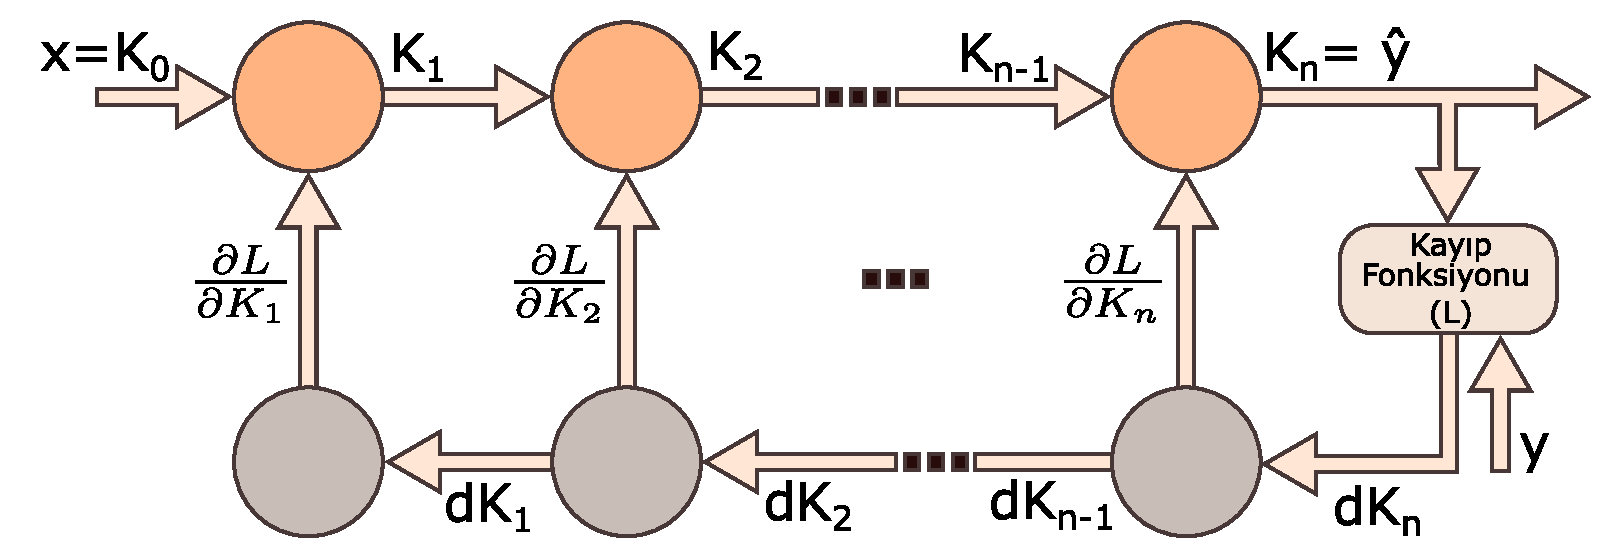
\includegraphics[scale=0.55]{Yapilan-Calismalar/Figures/backpropagation.pdf}
		}
	\end{center}
\end{figure}

Şekil \ref{fig:backpropagation}'te geri yayılım algoritmasında kısmi türevlerin hesaplanarak her katmandaki eğitilebilir parametrelerin güncellenebilmesi için zincir kuralı ile çıkış katmanından giriş katmanına doğru kısmı türev hesabının gerçekleştirilmesi gerektiği görülmektedir. Herhangi bir $m$ inci katmandaki eğitilebilir parametrelerin güncellenmesi için kullanılan kayıp fonksiyonundan elde edilen hataya göre kısmi türev hesabı Eşitlik \ref{eq:chain_rule}'de veridiği gibi hesaplanmaktadır.
\begin{equation}
	\label{eq:chain_rule}
	\frac{\partial L}{\partial  K_{m}} = \frac{\partial L}{\partial  K_{n}}\cdot\frac{\partial K_{n}}{\partial  K_{n-1}}\cdot...\cdot \frac{\partial K_{m+1}}{\partial  K_{m}}
\end{equation}

Her bir katmanda eğitilebilir katman parametrelerinin eğitimini gerçekleştirmek için hataya göre kısmi türevler hesaplanmakta ve hatanın minimize edilmesi için bu kısmi türev bilgisi kullanılmaktadır. Literatürde hatayı minimize edebilmek için kısmi türeve dayalı birçok optimizasyon tekniği mevcuttur. Bu optimizasyon tekniklerine bir sonraki bölümde değinilecektir.

\subsection{Geri Yayılım Algoritması Optimizasyon Teknikleri}
Geri yayılım algoritması kayıp fonksiyonu tarafından üretilen hatanın minimize edilmesini amaçlayan bir algoritmadır. Geri yayılım algoritmasında hatayı minimize etmek için eğitilebilir parametrelerin hataya göre kısmi türevini kullanan akıllı optimizasyon teknikleri derin ağın eğitim sürecini hızlandırabilmektedirler. 

Eğitilebilir tam bağlantılı katmanlardaki $W$, $b$ parametreleri ile konvolüsyon katmanlarındaki $F$ parametrelerinin herbiri için $\theta$ genel ifadesi kullanılmaktadır. Eğitilebilir $\theta$ parametresinin ağın toplam hatasına göre kısmi türevi Eşitlik \ref{eq:thetaderivative}'deki gibi ifade edilmektedir. İlgili $\theta$ parametresinde gerçekleştirilmesi gereken değişim kısmi hataya göre kısmi türev hesaplanılarak gerçekleştirilmektedir.
\begin{equation}
	\label{eq:thetaderivative}
	\frac{\partial}{\partial  \theta}L(\theta) = \nabla_{\theta}L
\end{equation} 

Kısmi türevin hatanın optimize edilmesindeki etkisi Şekil \ref{fig:gradyan}'da gösterilmektedir. Kısmi türev değerinin yönü hatanın minimize edilmesi için $\theta$ parametresinde gerçekleştirilmesi gereken negatif ya da pozitif yöndeki değişimin öngörülebilmesini sağlamaktadır.

\captionsetup[figure]{margin={0.5cm,-1cm}}
\begin{figure}[h!]
	\begin{center}
		\vspace{0.4cm}
		\captionbox{Gradyan bilgisinin hatanın minimize edilmesindeki etkisi.\label{fig:gradyan}}
		{
			\vspace{0.4cm}
			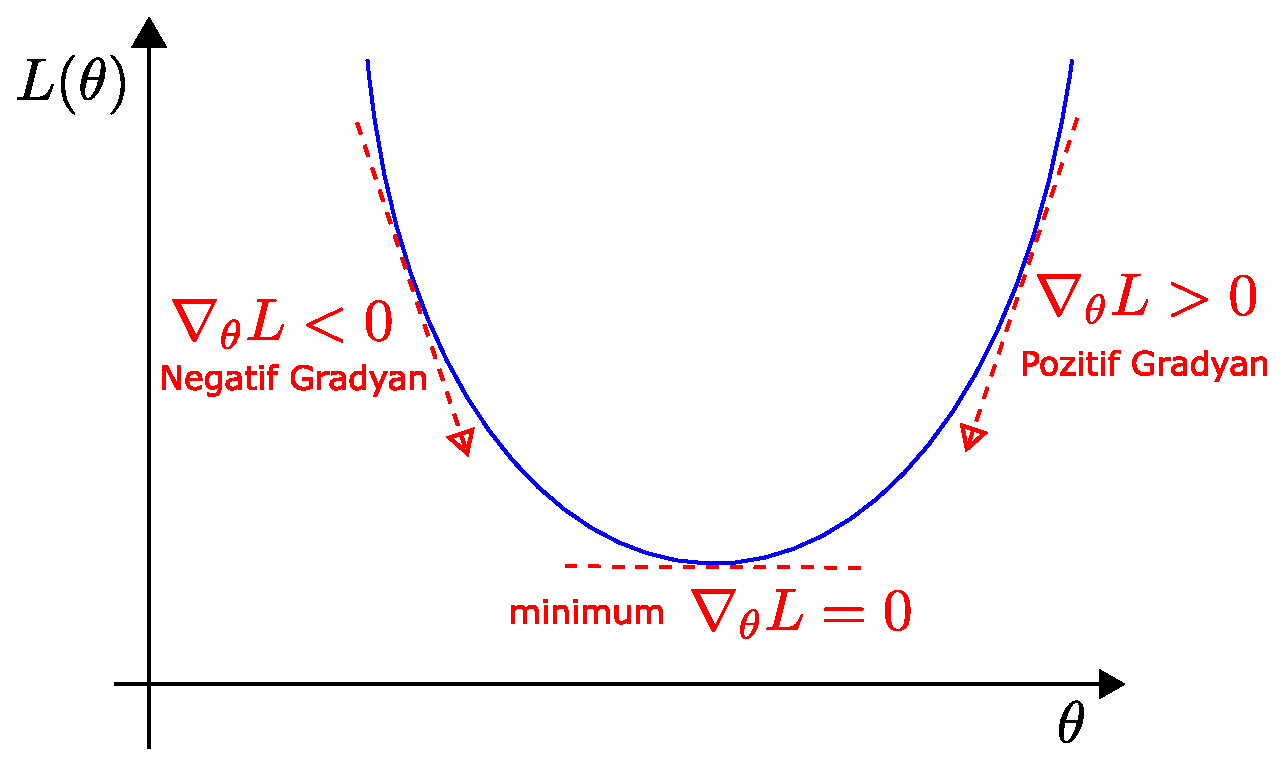
\includegraphics[scale=0.5]{Yapilan-Calismalar/Figures/gradyan.pdf}
		}
	\end{center}
\end{figure}

Çok katmanlı mimarilerde ağın eğitilmesi için genellikle bu gradyan bilgisinden faydalanan yöntemler tercih edilmektedir.

\subsubsection{Paket Gradyan Azalma}
Paket Gradyan Azalma (Batch Gradient Descent - BGD) yöntemi eğitimi tüm eğitim seti ile gerçekleştirmeyi öneren bir yaklaşımdır. BGD yöntemi hatayı minimize etmek için hesaplanan $\nabla_{\theta}L$ kısmi türevini bir $\alpha$ öğrenme katsayısı (learning rate) parametresi ile çarparak Eşitlik \ref{eq:batchgradiantdescent}'de görüldüğü gibi $\theta$ parametresine eklenilmesini önermektedir.
\begin{equation}
	\label{eq:batchgradiantdescent}
	\theta = \theta - \alpha \nabla_{\theta}L(\theta)
\end{equation} 

Öğrenme katsayısı bu yaklaşımda eğitimin başında bir kez atanmakta ve tüm eğitim boyunca aynı öğrenme katsayısıyla eğitim gerçekleştirilmektedir. Büyük veri kümelerinin eğitiminde tüm verinin eğitime tabi tutulmak zorunda olmasından dolayı hesaplama maliyeti oldukça yüksek bir yaklaşımdır.

\subsubsection{Mini-Paket Gradyan Azalma}
Mini-Paket Gradyan Azalma (Mini-Batch Gradient Descent) yöntemi Paket Gradyan Azalma yönteminin aksine tüm verinin değil paket boyutu (batch size) parametresine bağlı olarak verinin alt paketlere bölünerek eğitilmesini önermektedir. Bu sebeple bu yöntem eğitim her alt veri paketi için gerçekleştirilerek eğitim hesaplama maliyetinin düşürülmesi sağlanmaktadır. Tüm veri içinden $n$ adet alt veriyi seçerek Eşitlik \ref{eq:mbatchgradiantdescent}'te gösterildiği gibi hatanın optimize edilmesini hedeflemektedir.
\begin{equation}
	\label{eq:mbatchgradiantdescent}
	\theta = \theta - \alpha \nabla_{\theta}L(\theta;x^{(i:i+n)};y^{(i:i+n)})
\end{equation} 

Eğitimde tüm verinin kullanılmamasının sağladığı hız avantajının yanında eğitilebilir parametrelerin her küçük alt paket sonunda gerçekleştirdiği için eğitimin daha tutarlı olmasını sağlamaktadır.

\subsubsection{Stokastik Gradyan Azalma}
Stokastik Gradyan Azalma (Stochastic Gradient Descent - SGD) yöntemi tüm veri setiyle eğitimi gerçekleştirmek yerine her bir veri ile derin ağı tek tek eğitime tabi tutarak eğitilebilir parametrelerin güncellenmesini sağlamaktadır. Bu sebeple eğitim her örnek için ayrı ayrı gerçekleştirilmektedir. SGD yöntemi ile eğitilebilir parametrelerin eğitimi Eşitlik \ref{eq:sgradiantdescent}'te verildiği gibi gerçekleştirilmektedir.
\begin{equation}
	\label{eq:sgradiantdescent}
	\theta = \theta - \alpha \nabla_{\theta}L(\theta;x^{i};y^{i})
\end{equation} 
Her bir veri ile eğitim tek tek gerçekleştirildiği için hesaplama maliyeti oldukça yüksek bir yöntemdir.

\subsubsection{Momentumlu Stokastik Gradyan Azalma}
Momentumlu Stokastik Gradyan Azalma yöntemi temelinde hatanın gradyanının değişimindeki momentuma göre eğitim gerçekleştirmektedir. Optimizasyonun temel fizik kuramından destek alınarak gerçekleştirildiği bu yaklaşımda hatanın eğimi çok yüksek olduğunda fazla ivme kazandırılarak eğitimin lokal minimumlara takılmasının önüne geçilmektedir. Eğimdeki değişim azaldıkça ivme azaltılarak hatanın optimizasyonu sağlanmaktadır.

Momentumlu Stokastik Gradyan Azalma yöntemi standart SGD optimizasyon yöntemi modifiye edilerek geliştirilmiştir. Eğitilebilir $\theta$ parametrelerinin güncellenmesi Eşitlik \ref{eq:msgradiantdescent}'te görüldüğü gibi gerçekleştirilmektedir. Bu teknikte ivmenin kontrolü $\upsilon$ hız parametresi ile, hızın kontrolü ise $\mu$ sürtünme parametresi (momentum) ile gerçekleştirilerek global minimumu yakalamak hedeflenmektedir.
\begin{equation}
	\label{eq:msgradiantdescent}
	\begin{array}{ r l }
		\upsilon = &  \mu\upsilon - \alpha \nabla_{\theta}L(\theta) \\
		\theta = & \theta + \upsilon
	\end{array}
\end{equation}

Momentumlu Stokastik Gradyan Azalma yönteminde SGD yöntemine göre çok küçük bir değişiklik olmasına rağmen öğrenme hızında SGD yönteminden çok büyük bir artış söz konusudur.

\subsubsection{Adaptif Gradyan Algoritması}
Adaptif Gradyan Algoritması (Adaptive Gradient - AdaGrad) SGD algoritmasının her eğitilebilir parametreye özgü öğrenme katsayısı kullanma mantığı ile geliştirilmiş bir optimizasyon yöntemidir \cite{duchi2011adaptive}. Az karşılaşılan parametrelerin daha önemli bilgiler barındırabileceği mantığını savunan AdaGrad yönteminde öğrenme katsayısı $\alpha$ daha nadir rastlanan parametrelerde artırılırken daha sık rastlanan parametrelerde düşürülmektedir. 

AdaGrad algoritmasında eğitim sürecinde öğrenme katsayısı $\alpha$ kullanılmakta ve $\tau$ inci iterasyondaki hatanın kısmi türevi $g_{\tau}=\nabla L(\theta)$ olmak üzere, $\alpha$ öğrenme katsayısı değeri $G=\sum_{\tau=1}^{t} g_{\tau} g_{\tau}^{\mathrm{T}}$ dış çarpım matrisinin diyagonali olan $\left\{G_{j, j}\right\}$ vektörü ile çarpılmaktadır. $G_{j, j}=\sum_{\tau=1}^{t} g_{\tau, j}^{2}$ vektörü her iterasyonda güncellenmekte ve $\theta$ eğitilebilir parametrelerinin güncellenmesi Eşitlik \ref{eq:adagrad}'da verildiği gibi gerçekleştirilmektedir. Böylece her eğitilebilir $\theta_{i}$ parametresi için bir ölçekleme faktörü belirlenmiş olmaktadır. \begin{equation}
	\label{eq:adagrad}
	\theta_{j} = \theta_{j}-\frac{\alpha}{\sqrt{G_{j, j}}} g_{j}
\end{equation}

\subsubsection{Ortalama Karekök Yayılım Algoritması}
Ortalama Karekök Yayılım algoritması (Root Mean Square Propagation - RMSProp), sinir ağlarının eğitiminde kullanılan gradyan tabanlı optimizasyon tekniklerinden birisidir \cite{tieleman2012lecture}. RMSprop tekniği mini-paket öğrenme için geliştirilmiş bir stokastik tekniktir. RMSprop tekniği gradyanı normalleştirmek için kare gradyanların hareketli ortalamasını kullanarak kaybolan gradyan problemini ortadan kaldırmayı amaçlamaktadır. RMSprop tekniğindeki ana fikir, eğitilebilir bir parametre için öğrenme oranını, o ağırlık için son gradyanların büyüklüklerinin değişen bir ortalamasına bölmektir. Bu nedenle, unutma faktörü $\beta$ olarak temsil edilmek üzere öncelikle gradyanların ortalaması ortalama karekök cinsinden Eşitlik \ref{eq:rmsprop1}'deki gibi hesaplanmaktadır.
\begin{equation}
	\label{eq:rmsprop1}
	v(\theta, t)=\beta v(\theta, t-1)+(1-\beta)\left(\nabla L_{i}(\theta)\right)^{2}
\end{equation}
Daha sonra eğitilebilir parametreler bu değer ile Eşitlik \ref{eq:rmsprop2}'de görüldüğü gibi güncellenmektedir.
\begin{equation}
	\label{eq:rmsprop2}
	\theta=\theta-\frac{\alpha}{\sqrt{v(\theta, t)}} \nabla L_{i}(\theta)
\end{equation}

\subsubsection{Adaptif Moment Tahmini Algoritması}
RMSprop yönteminin geliştirilmiş bir versiyonu olan Adaptif Moment Tahmini algoritması (Adaptive Moment Estimation - Adam) düşük mertebeden momentlerin uyarlanabilir tahminlerine dayanmaktadır. Bu algoritma stokastik amaç fonksiyonlarının birinci mertebeden gradyan tabanlı bir optimizasyon tekniğidir \cite{kingma2014adam}. Adam, günümüzde en çok tercih edilen ve en son teknoloji optimizasyon algoritmalarından biridir. Bu tez çalışmasında da Adam optimizasyon yöntemi tercih edilmiştir. 

Bu optimizasyon algoritmasında hem gradyanların hem de gradyanların ikinci momentlerinin ortalamaları kullanılmaktadır. İkinci moment tarafından normalleştirilen ilk moment güncellemenin yönünü vermektedir. Eğitimde $t$ mevcut eğitim iterasyonu indeksi, $\theta^{(t)}$ eğitilebilir parametreler ve $L^{(t)}$ kayıp fonksiyonu olmak üzere, Adam algoritmasının eğitilebilir parametre güncellemesi Eşitlik \ref{eq:adam5}'te verildiği gibi hesaplanmaktadır.
\begin{equation}
	\label{eq:adam1}
	m_{\theta}^{(t+1)} \leftarrow \beta_{1} m_{\theta}^{(t)}+\left(1-\beta_{1}\right) \nabla_{\theta} L^{(t)}
\end{equation}
\vspace{-1cm}
\begin{equation}
	\label{eq:adam2}
	v_{\theta}^{(t+1)} \leftarrow \beta_{2} v_{\theta}^{(t)}+\left(1-\beta_{2}\right) (\nabla_{\theta} L^{(t)})^{2}
\end{equation}
\vspace{-1cm}
\begin{equation}
	\label{eq:adam3}
	\hat{m}_{\theta}=\frac{m_{\theta}^{(t+1)}}{1-\beta_{1}^{t}}
\end{equation}
\vspace{-1cm}
\begin{equation}
	\label{eq:adam4}
	\hat{v}_{\theta}=\frac{v_{\theta}^{(t+1)}}{1-\beta_{2}^{t}}
\end{equation}
\vspace{-1cm}
\begin{equation}
	\label{eq:adam5}
	\theta^{(t+1)} = \theta^{(t)}-\alpha \frac{\hat{m}_{\theta}}{\sqrt{\hat{v}_{\theta}}+\epsilon}
\end{equation}

Adam optimizasyon tekniği formülizasyonunda $\alpha$ öğrenme katsayısı, $\beta_{1}$, $\beta_{2}$ unutma faktörü parametreleridir. $\epsilon$ ifadesi sıfıra bölünme hatasına yakalanmamak için sıfıra çok yakın küçük bir değer seçilmelidir.

\subsection{Derin Ağlarda Düzenleştirme}
Derin ağlarda modelin eğitiminin yeterli yapılmadığı ya da giriş verilerinin eğitimi gerçekleştirmek istediğimiz veri setini tam ifade edemediği, eksik eğitim verilerinin kullanıldığı gibi durumlarda eksik uyum (underfitting) durumu ortaya çıkmaktadır. Aynı zamanda eğitimin gereğinden fazla sürdürüldüğü durumlarda da model eğitim setindeki her bir örneği eksiksiz öğrenmeye çalışmakta ve problemi eğitim seti için mükemmel öğrenmiş gibi görünse de test setinde büyük hatalar yapılmasına sebebiyet veren aşırı öğrenme (overfitting) durumu ile karşılaşılmaktadır. Eğitimde amaç eğitim seti eğitiminin genelleştirilerek doğru öğrenmenin sağlanmasıdır. Eksik uyum, doğru uyum ve aşırı uyum durumları Şekil \ref{fig:regularization}'de gösterilmektedir.
\captionsetup[figure]{margin={0.5cm,-1cm}}
\begin{figure}[h!]
	\begin{center}
		\vspace{0.4cm}
		\captionbox{Modelin eksik öğrenmesi, doğru öğrenmesi ve aşırı öğrenmesi durumları.\label{fig:regularization}}
		{
			\vspace{0.4cm}
			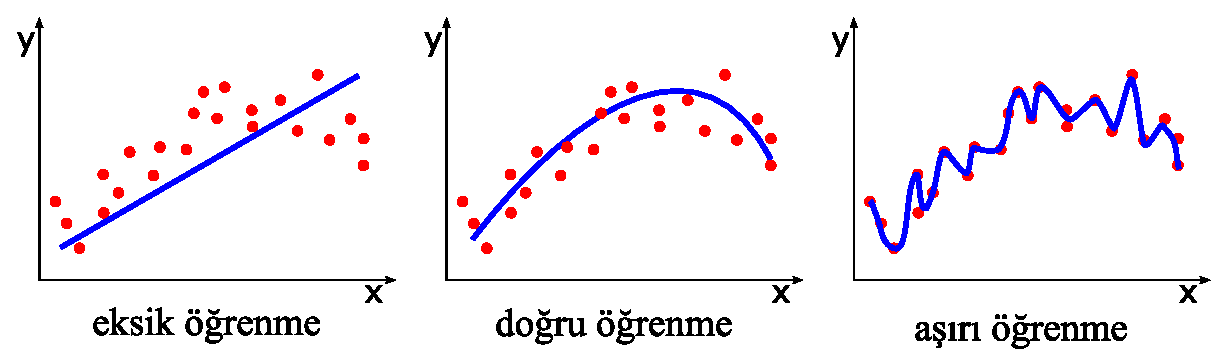
\includegraphics[scale=0.65]{Yapilan-Calismalar/Figures/regularization.pdf}
		}
	\end{center}
\end{figure}

Derin öğrenmede uyum problemlerini ortadan kaldırmak için literatürde birçok yöntem önerilmiştir \cite{girosi1995regularization}. Düzenleştirme işlemini gerçekleştiren katmanlardan olan Seyreltme katmanları ve Paket Normalizasyon katmanları sırasıyla Bölüm \ref{lyr:dropout} ve \ref{lyr:batchnormalization}'da incelenmiştir. Bu yöntemler haricinde literatürde Veri Artırma \cite{shorten2019survey}, L1 ve L2 Düzenleştirme \cite{ng2004feature} işlemleri de kullanılmaktadır.

\subsubsection{Veri Artırma} 
Derin ağlarda giriş verisi üzerinde gerçekleştirilen düzenleme yöntemlerinden birisidir. Derin öğrenmede eğitim verisi üzerinden iyi bir genelleştirme yapabilmek için çok sayıda görüntüye ihtiyaç duyulmaktadır. Veri artırma az sayıdaki giriş veri setini bazı transformasyon işlerine tabi tutarak artırmayı öneren bir yaklaşımdır. Veri artırmada öteleme, yansıtma, döndürme, ölçekleme, gürültü ekleme, kırpma gibi oldukça zengin transformasyon işlemleri kullanılabilmektedir. Şekil \ref{fig:augmentation}'de veri artırma tekniği ile farklı transformasyonlarda eğitim verisinin çoğaltılması gösterilmektedir. Derin ağlarda özellik çıkarma işlemi otomatikleştirildiği için çok sayıda görüntü ile genelleştirme yapmak çok daha güçlü özellik haritaları elde etmemizi sağlamaktadır. 

Veri artırmayı uygularken verinin transformasyon sonrası farklı bir sınıfa benzememesine dikkat etmek gerekmektedir. Örneğin el yazısı rakam sınıflandırmada veri artırma gerçekleştirirken döndürme transformasyonu 6 ve 9 rakamların birbiri ile karışmasına sebep olmaktadır. Ayrıca BT verisi gibi 2B dilimlerden oluşan 3B veri setlerinde kullanılan transformasyon tüm alt dilimler için aynı şekilde uygulanmalıdır. Segmentasyon problemlerinde de yine transformasyon hem giriş verisine hemde eğitim maske verilerine aynı şekilde uygulanmalıdır.

\captionsetup[figure]{margin={0.3cm,-0.5cm}}
\begin{figure}[h!]
	\begin{center}
		\vspace{0.4cm}
		\captionbox{Veri artırma tekniği ile farklı transformasyonlarda eğitim verisinin çoğaltılması.\label{fig:augmentation}}
		{
			\vspace{0.4cm}
			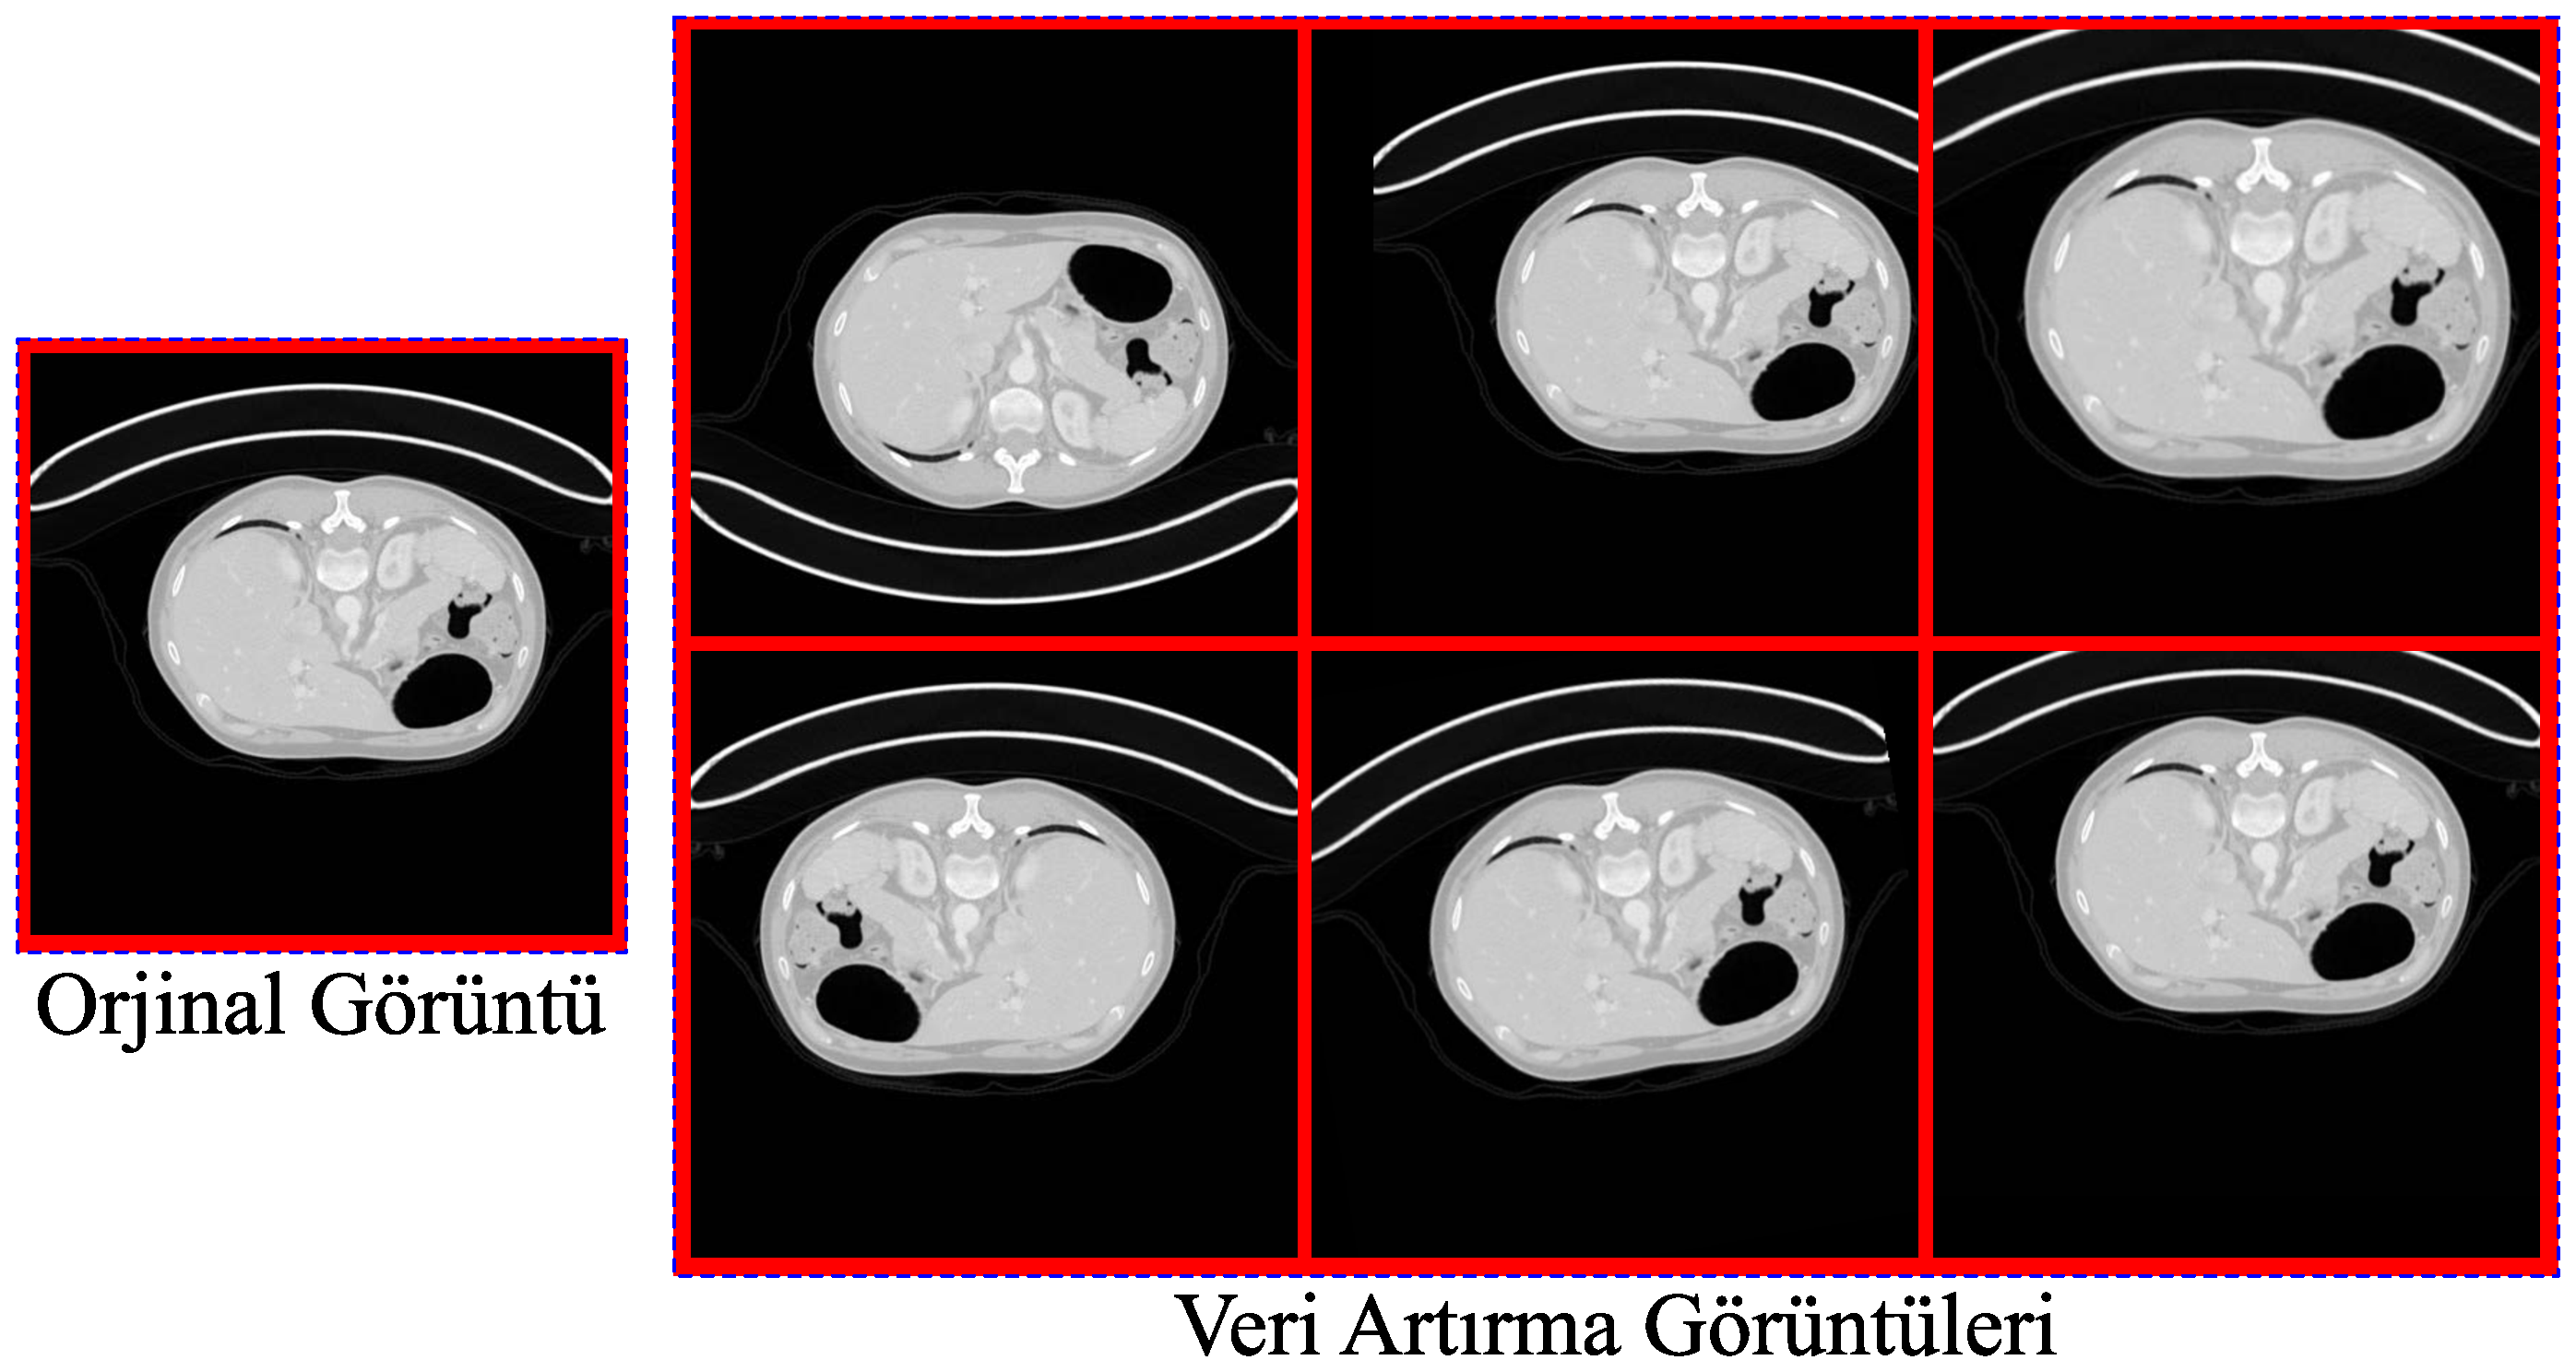
\includegraphics[scale=0.3]{Yapilan-Calismalar/Figures/augmentation.pdf}
		}
	\end{center}
\end{figure}

\subsubsection{L1 ve L2 Düzenleştirme} 
L1 ve L2 düzenleştirmeler aşırı öğrenmenin önüne geçebilmek için tam bağlantılı katmanlardaki eğitilebilir ağırlık $w$ ve yanlılık $b$ parametrelerini $\theta$ genel adıyla tanımlamak üzere sırasıyla Eşitlik \ref{eq:l1reg} ve \ref{eq:l2reg}'te verildiği gibi hesaplanmaktadır.
\begin{equation}
	\label{eq:l1reg}
	L_{1 \theta}=\lambda \sum_{m}\left|\theta_{m}\right|
\end{equation}
\vspace{-1cm}
\begin{equation}
	\label{eq:l2reg}
	L_{2 \theta}=\lambda \sum_{m}\theta_{m}^{2}
\end{equation}
Tam bağlantılı katmandaki eğitilebilir parametreler için tanımlanan cezalandırma katsayısı $\lambda$ ağırlık $w$ ve yanlılık $b$ değerleri için ayrı ayrı tanımlanarak $L_{1w}$, $L_{2w}$, $L_{1b}$ ve $L_{2b}$ değerleri hesaplanabilmektedir. Hesaplanan bu L1 ve L2 cezalar ağın genel hatasına Eşitlik \ref{eq:l1l2reg}'daki gibi eklenerek eğitim gerçekleştirilmektedir. Böylece ağın genel hata değeri ($L$) L1 ve L2 düzenleştirme değerleri ile cezalandırılmaktadır. 
\begin{equation}
	\label{eq:l1l2reg}
	L = L + L_{1w} + L_{2w} + L_{1b} + L_{2b}
\end{equation}

%%%%%%%%%%%%%%%Önerilen Yöntem%%%%%%%%%%%%%%%%%%%%%%
\section{Pankreas İlgi Bölgesinin Belirlenmesi ve İlgi Bölgesinde Pankreas Segmentasyonu \label{sec:pancreas}}

Bu tez çalışmasında BT görüntülerinde bulunan, abdominal bölgede oldukça küçük bir alan kaplayan pankreas organının daha başarılı segmentasyonu hedeflenmektedir. Bu hedef için tez çalışmasında kabadan inceye yöntemi ile pankreas ilgi bölgesinin belirlenmesi ve bu ilgi bölgesinde pankreas segmentasyonunun gerçekleştirilmesine yönelik bir yaklaşım önerilmektedir. Bu yaklaşım Pankreas İlgi Bölgesinin   Belirlenmesi ve İlgi Bölgesinde Pankreas Segmentasyonu olmak üzere Şekil \ref{fig:proposed_aproach}'da gösterildiği gibi iki fazdan oluşmaktadır.

\captionsetup[figure]{margin={0.3cm,-0.3cm}}
\begin{figure}[h!]
	\begin{center}
		\vspace{0.4cm}
		\captionbox{ Pankreas Segmentasyonu için önerilen 2 fazlı (Pankreas İlgi Bölgesinin Belirlenmesi, Belirlenen İlgi Bölgesinde Pankreas Segmentasyonu) yöntemin blok diyagramı.\label{fig:proposed_aproach}}
		{
			\vspace{0.4cm}
			\includegraphics[scale=0.695]{Yapilan-Calismalar/Figures/proposed_aproach.pdf}
		}
	\end{center}
\end{figure}

Yaklaşımın birinci fazında kaba pankreas bölgesinin tespiti için 2B segmentasyon yöntemlerinden olmasına karşın oldukça başarılı segmentasyon sonuçları üretebilen Mask R-CNN yöntemi tercih edilmektedir. Hasta bireylerin abdominal bölgelerinden çekilen ham 3B volümetrik BT verilerinin her bir 2B alt dilimi daha önce eğitim veri seti ile eğitilmiş Mask R-CNN modeline ayrı ayrı verilerek 2B segmentasyon gerçekleştirilmektedir. Segmentasyonu gerçekleştirilen her bir BT diliminin birleştirilmesi ile elde edilen 3B volümetrik veriden pankreas organının ilgi bölgesi kaba hatları ile belirlenmektedir. Kaba pankreas bölgesinde 2B bir yöntem tercih edilerek hesaplama yükünün düşürülmesi sağlanmaktadır.

Yaklaşımın ikinci fazında belirlenen ilgi bölgesi üzerinde 3B U-Net yöntemi ile tekrar segmentasyon gerçekleştirilerek pankreas organının daha hassas segmentasyonu gerçekleştirilmektedir. Hassas segmentasyon aşamasında bölgenin küçülmesinden kaynaklı hesaplama yükünün azalması ile 3B yöntemlerin kullanılabilir olması sağlanmaktadır. Böylece dilimler arasındaki süreklilik bilgisi dikkate alınarak daha hassas segmentasyon işlemi gerçekleştirilebilmektedir.

\subsection{Pankreas İlgi Bölgesinin Belirlenmesi}
Önerilen otomatik pankreas segmentasyon yaklaşımının ilk fazı olan Pankreas İlgi Bölgesinin Belirlenmesi, ($512 \times 512 \times N$) boyutundaki 2B BT dilimlerini giriş olarak almaktadır. Burada $N$, BT taramasındaki dilim sayısını temsil etmektedir. 2B alt BT dilimlerini ($256 \times 256 \times 2N / 3$) çıkış olarak üretmektedir. Pankreas İlgi Bölgesinin Belirlenmesi fazı, pankreas segmentasyonu için işlenen BT dilimlerinin boyutunu azaltmayı amaçlamaktadır. Bu faz Mask R-CNN ile Pankreas İlgi Bölgesinin Belirlenmesi ve Mask R-CNN'den elde edilen bilgi ile Kaba Pankreas Bölgesinin Belirlenmesi olmak üzere iki ana aşamadan oluşmaktadır.
 
\subsubsection{Mask R-CNN Modeli ile İlgi Bölgesinin Belirlenmesi}
Pankreas İlgi Bölgesinin Belirlenmesi aşamasında 2B BT dilimlerindeki ($512 \times 512 \times N$) kaba pankreas bölgelerinin tespit edilmesine odaklanılmıştır. Bu aşamada, Mask R-CNN yöntemi kullanılarak, 2B BT dilimlerinden hem sınırlayıcı kutuları elde edilmekte hem de kaba pankreas bölgelerinin bölümlere ayrılmış alt görüntüleri segmente edilmektedir.

\captionsetup[figure]{margin={0.4cm,-0.5cm}}
\begin{figure}[h!]
	\begin{center}
		\vspace{0.4cm}
		\captionbox{Pankreas İlgi Bölgesinin Belirlenmesi fazının Mask R-CNN modeli kullanan ilk aşamasındaki beş ana adımın şematik gösterimi.\label{fig:maskrcnn}}
		{
			\vspace{0.4cm}
			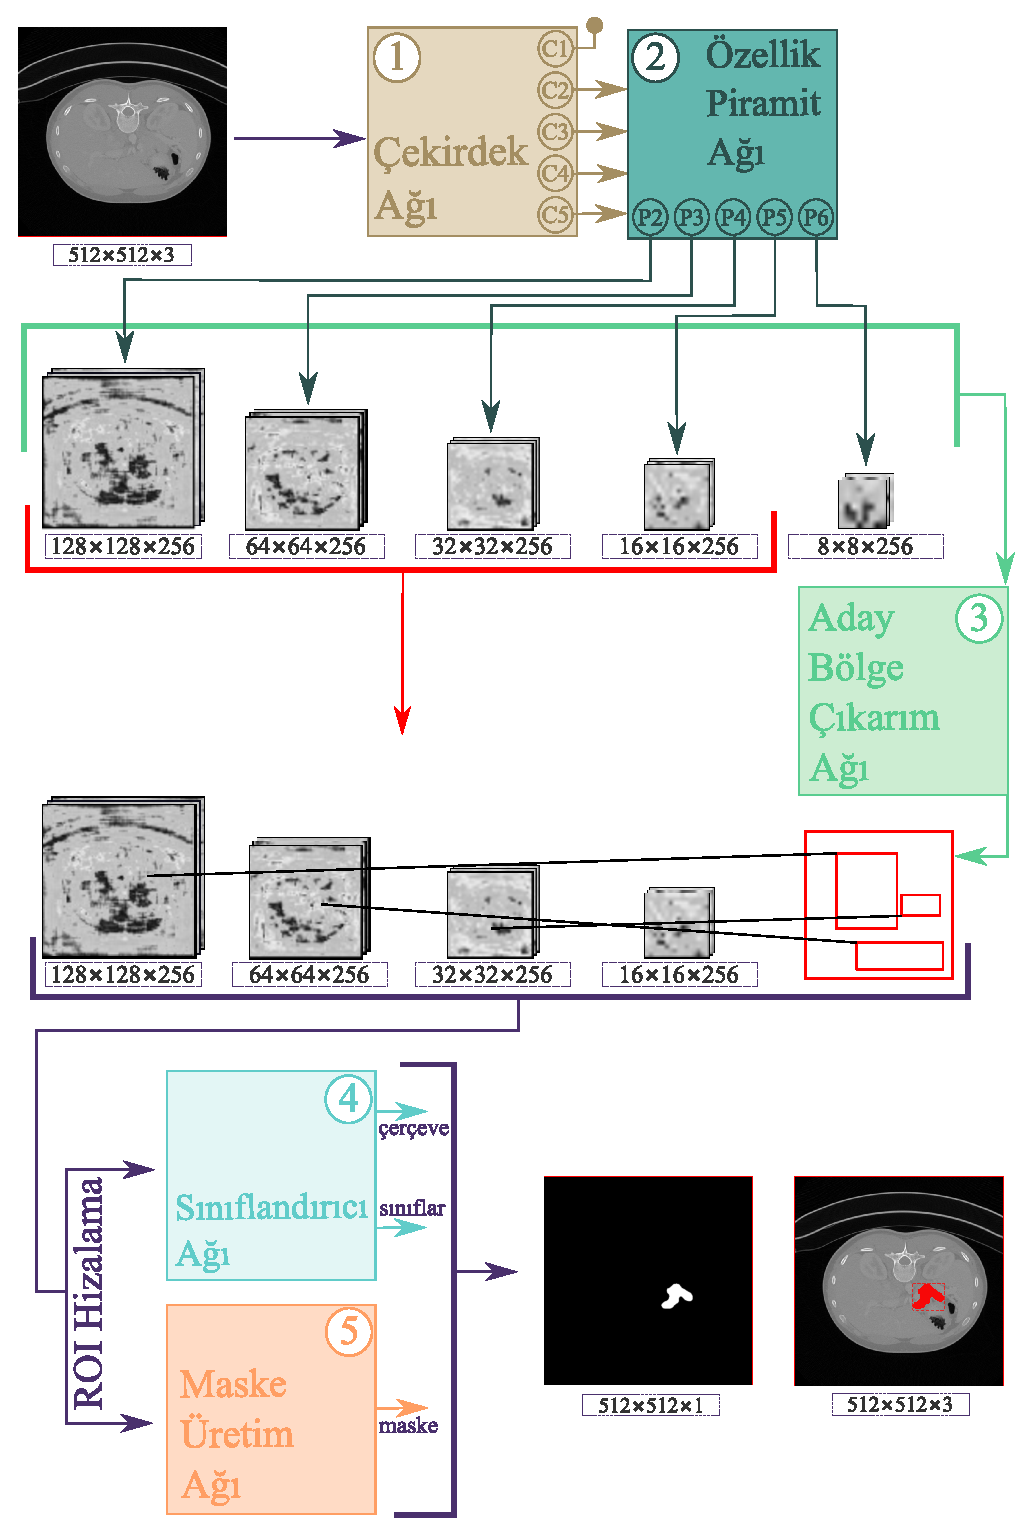
\includegraphics[scale=0.8]{Yapilan-Calismalar/Figures/maskrcnn.pdf}
		}
	\end{center}
\end{figure}

He tarafından 2018 yılında geliştirilen Mask R-CNN modeli \cite{he2017mask}, 2B nesne segmentasyonu için en güçlü yöntemlerden biridir. Bu model çok sınıflı nesne algılama için oldukça yüksek doğruluklu ve gerçek zamanlı performans sağlamaktadır. Bu model Hızlandırılmış Bölge Esaslı Konvolüsyonel Sinir Ağları \cite{ren2015faster} (Faster Region Proposal Convolutional Neural Network - Faster R-CNN) modelinin geliştirilmiş versiyonudur. Mask R-CNN modeli, Faster R-CNN modeline ek olarak maske üretimi ve sınıflandırıcı ağlardan oluşmaktadır. Mask R-CNN modelini diğer segmentasyon yöntemlerinden ayıran en önemli özelliği, görüntüdeki her nesnenin hem sınırlayıcı kutularını hem de segmentasyon sonuçlarını üretebilmesidir. 

Şekil \ref{fig:maskrcnn}’da Pankreas İlgi Bölgesinin Belirlenmesi fazının Mask R-CNN modeli kullanan ilk aşamasındaki beş ana adımın şematik gösterimi verilmektedir. Şekilde görüldüğü gibi Mask R-CNN modeli, Çekirdek Ağı (Head Network), Özellik Piramit Ağı (Feature Pyramid Network), Aday Bölge Çıkarım Ağı (Region Proposal Network), Sınıflandırıcı Ağı (Classifier Network) ve Maske Üretim Ağı (Mask Generation Network) olmak üzere beş ana adımdan oluşmaktadır. Pankreas İlgi Bölgesinin Belirlenmesi fazının Mask R-CNN modelini kullanan ilk aşamasında uygulanan ana adımlar şu şekilde açıklanabilmektedir.

\paragraph{Mask R-CNN Derin Ağ Modelinin Alt Ağlarından Çekirdek Ağı'nın Yapısı}

Kenar, doku ve renk kümesi bilgileri gibi 2B BT dilimlerinin spesifik özelliklerini tanımlamak için bu adımda Çekirdek Ağı (Head Network) oluşturulmaktadır. Bu tez çalışmasında Mask R-CNN Çekirdek Ağı olarak ResNet-101 CNN özellik çıkarıcı modelli ImageNet ağırlıkları ile transfer öğrenme tekniği kullanılarak denenmektedir. Tez çalışmasında kullanılan ResNet-101 modelli için Çekirdek Ağı'nın genel yapısı Şekil \ref{fig:head_network}’de verilmektedir. Bu ağ BT görüntüsünün tümünü $(512 \times 512 \times 3)$ giriş olarak almaktadır. Şekil \ref{fig:head_network}’de görüldüğü gibi giriş görüntüsünden C1, C2, C3, C4 ve C5 olarak adlandırılan beş farklı özellik haritası oluşturmaktadır. Bu özellik haritaları C1 için 128 x 128 x 64, C2 için 128 x 128 x 256, C3 için 64 x 64 x 512, C4 için 32 x 32 x 1024 ve C5 için 16 x 16 x 2048 olmak üzere farklı boyutlara sahiptirler. 

\captionsetup[figure]{margin={0.3cm,-2.5cm}}
\begin{figure}[h!]
	\begin{center}
		\vspace{0.4cm}
		\captionbox{ResNet-101 modeli kullanan Çekirdek Ağı'nın genel yapısı. \label{fig:head_network}}
		{
			\vspace{0.4cm}
			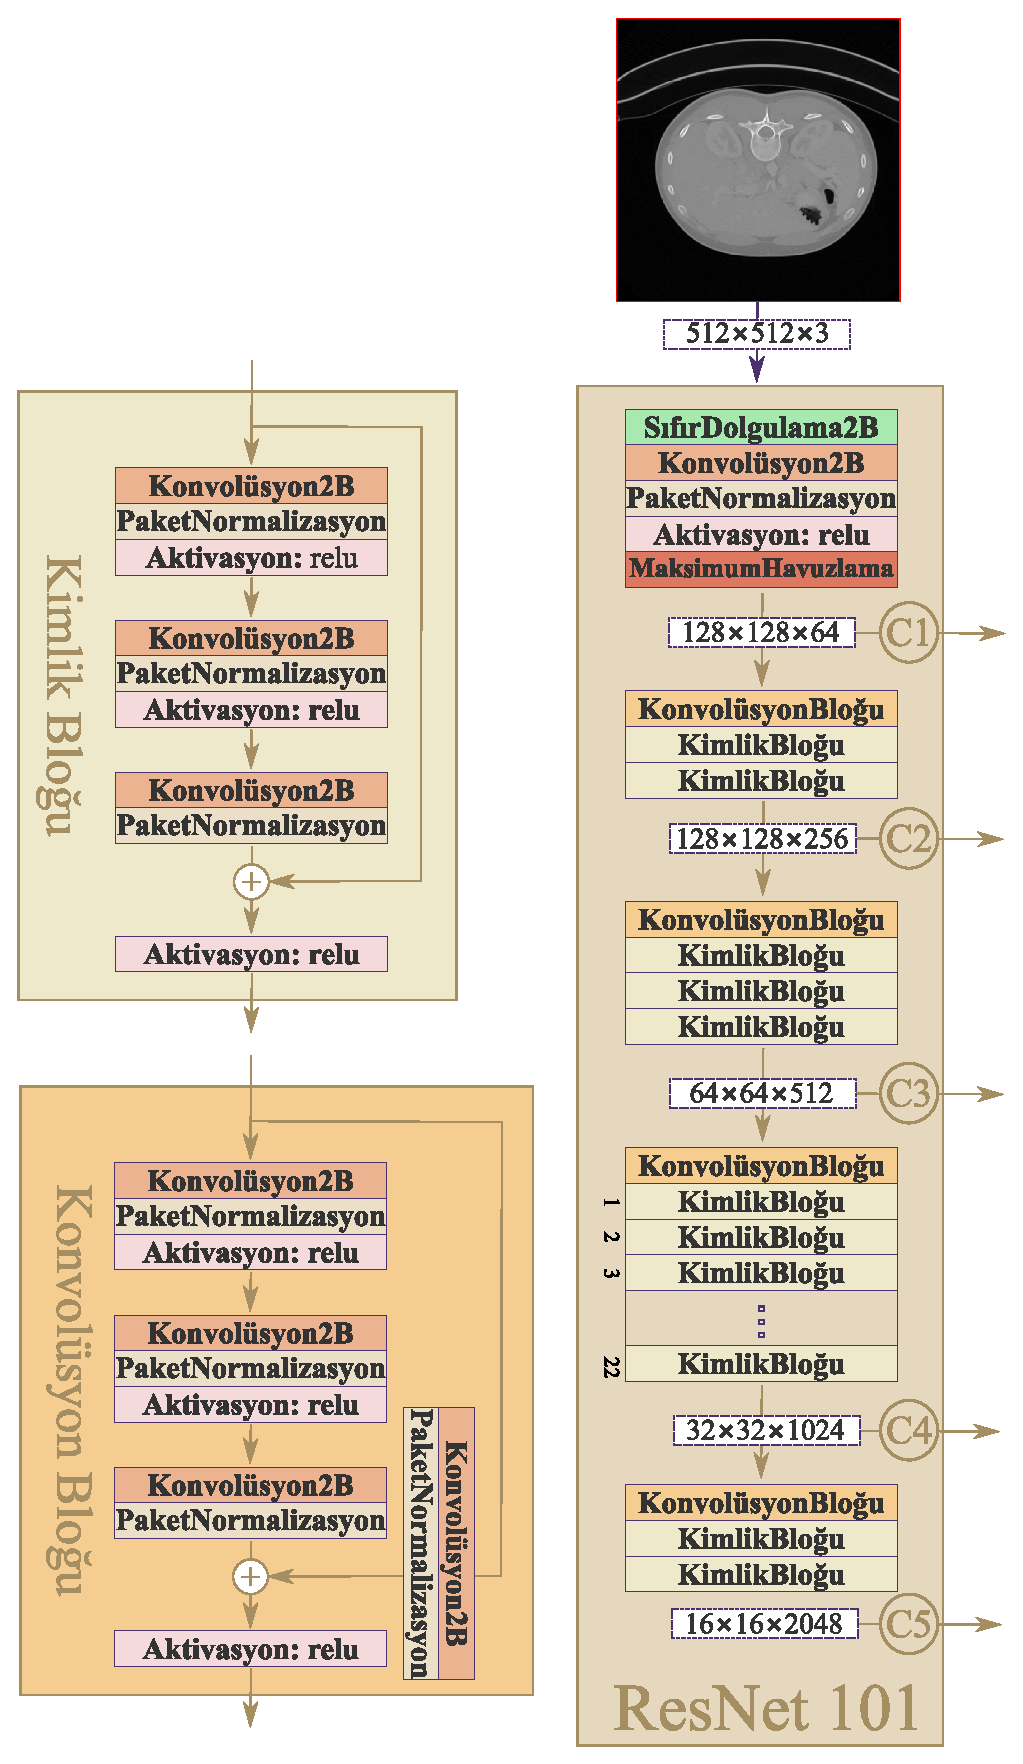
\includegraphics[scale=0.7]{Yapilan-Calismalar/Figures/head_network.pdf}
		}
	\end{center}
\end{figure}

ResNet mimarisi literatürde katman sayısını artırabilmek için artık (residual) bağlantıları kullanma fikri ile ortaya çıkarılmıştır \cite{he2016deep}. Böylece önceki katmanlardan gelen bilgi konvolüsyon işlemi sonrası katmanlarla birleştirilerek konvolüsyon işleminden kaynaklı bilgi kaybının önüne geçilebilmektedir. Eğitim hızını artırmak için Çekirdek Ağı'nda kullanılan ResNet-101 mimarisine transfer öğrenme tekniği kullanılarak ImageNet ağırlıkları ile ön yükleme işlemi gerçekleştirilmektedir. 

Çekirdek Ağı olarak kullanılan ResNet-101 mimarisi Şekil \ref{fig:head_network}’de görüldüğü gibi sıfır dolgulama (zero padding), 2B konvolüsyon (Convolutional), paket normalizasyon (Batch Normalization), doğrultulmuş doğrusal birim (RELU) ve maksimum havuzlama (Max Pooling) olmak üzere beş temel derin öğrenme katmanından oluşmaktadır. Ek olarak, Çekirdek Ağı'nda konvolüsyon (Convolutional) ve kimlik (identity) olmak üzere iki blok bulunmaktadır. Konvolüsyon ve kimlik blokları 2B konvolüsyon, paket normalizasyon ve RELU katmanlarını içermektedirler. Bu bloklar paket normalizasyonu katmanının çıkışına giriş ekleyerek kaybolan gradyan problemini ortadan kaldırmaktadırlar \cite{he2016deep}.

\paragraph{Mask R-CNN Derin Ağ Modelinin Alt Ağlarından Özellik Piramit Ağı'nın Yapısı}

Farklı ölçeklerde nesneleri algılamak nesne ölçeği azaldıkça zorlaşmaktadır. Bu amaçla görüntünün farklı ölçeklerdeki piramiti oluşturularak nesne tespiti farklı ölçeklerde gerçekleştirilebilmektedir. Farklı ölçeklerdeki görüntü piramitlerini işlemek oldukça fazla işlemci zamanı ve bilgisayar belleği tüketilmesine sebep olmaktadır. Bunun yerine görüntünün farklı ölçeklerdeki özellik haritalarında bu işlemi gerçekleştirmek çok daha efektif olmaktadır. Özellik Piramit Ağı (Feature Pyramid Network - FPN) bu amaç için geliştirilmiş derin özellik çıkarım modelidir \cite{lin2017feature}.  

\captionsetup[figure]{margin={0.5cm,-3cm}}
\begin{figure}[h!]
	\begin{center}
		\vspace{0.4cm}
		\captionbox{Özellik Piramit Ağı'nın genel  yapısı.\label{fig:feature_pyramid_network}}
		{
			\vspace{0.4cm}
			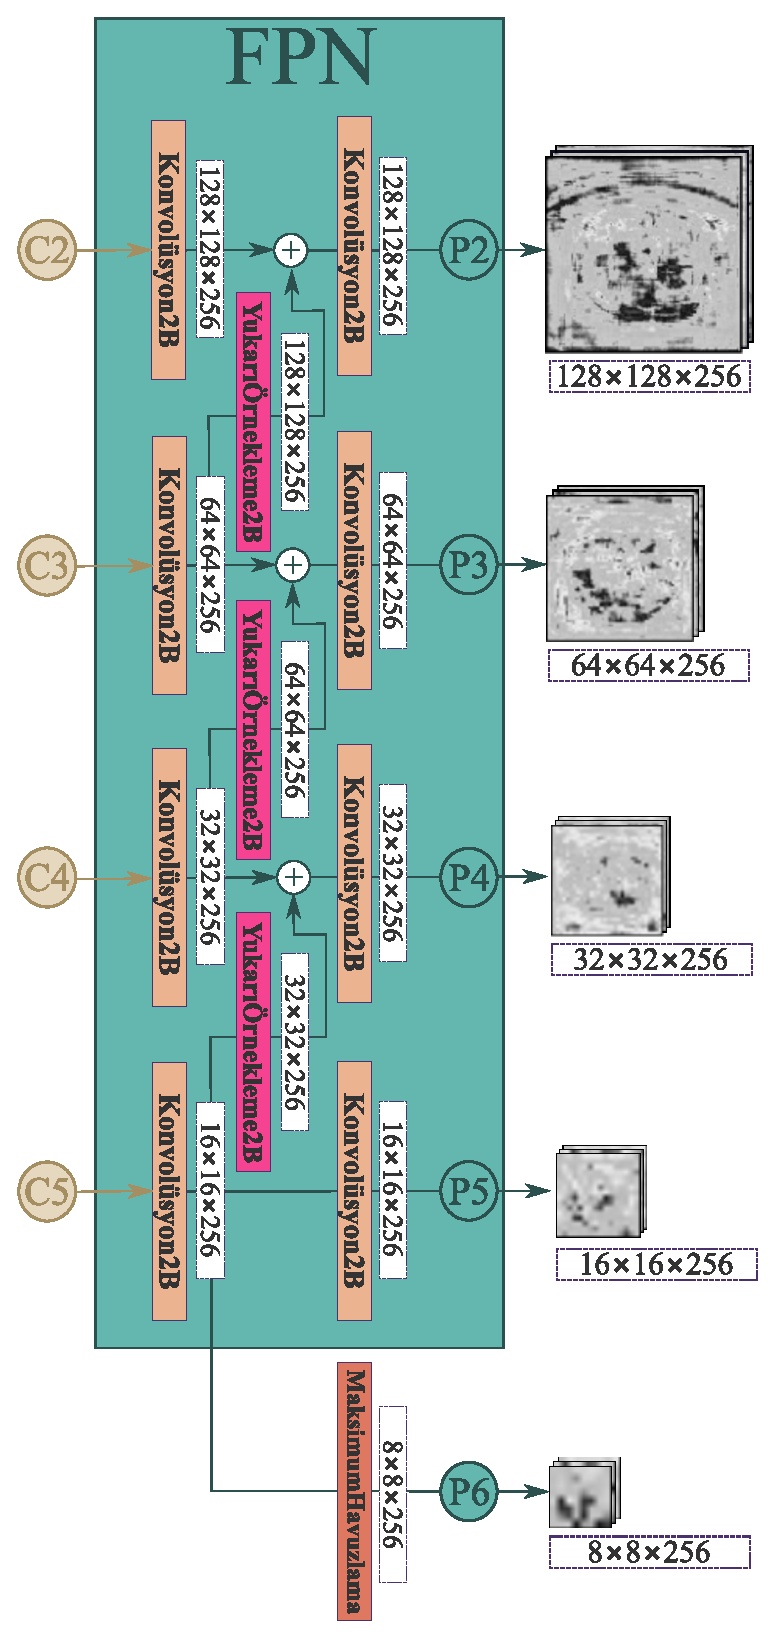
\includegraphics[scale=0.72]{Yapilan-Calismalar/Figures/feature_pyramid_network.pdf}
		}
	\end{center}
\end{figure}

2B BT dilimlerinin daha belirgin özelliklerini çıkarmak için, bu adımda Özellik Piramit Ağı oluşturulmaktadır. Özellik Piramit Ağı'nın genel yapısı Şekil \ref{fig:feature_pyramid_network}’de verilmektedir. Şekil \ref{fig:feature_pyramid_network}’de görüldüğü gibi Özellik Piramit Ağı, Çekirdek Ağı tarafından üretilen ($C2$ - $128 \times 128 \times 256$, $C3$ - $64 \times 64 \times 512$, $C4$ - $32 \times 32 \times 1024$ ve $C5 - 16 \times 16 \times 2048)$ dört farklı özellik haritasını giriş olarak almaktadır. Bu ağ yukarıdan aşağı yol (top-down pathway) adı verilen bir yaklaşım kullanarak beş farklı piramit özellik haritasını ($P2$ - $128 \times 128 \times 256$, $P3$ - $64 \times 64 \times 256$, $P4$ - $32 \times 32 \times 256$, $P5 - 16 \times 16 \times 256$ ve $P6$ - $8 \times 8 \times 256$) çıktı olarak üretmektedir. Yukarıdan aşağı yol yaklaşımında, yukarı ölçekli operasyonlar en küçük ölçekli özellik haritasından ($C5$) başlayarak en büyük ölçekli özellik haritasına doğru uygulanmaktadır. Yukarıdan aşağı yol yaklaşımı Çekirdek Ağı'nın farklı ölçeklerdeki konvolüsyon özellik haritalarını temsil etmektedir. Serideki özellik haritası sayısını $256$’ya düşürmek için Şekil \ref{fig:feature_pyramid_network}’de verildiği gibi ilk olarak Çekirdek Ağı’nda üretilen özellik haritaları ($C2$, $C3$, $C4$ ve $C5$) $1 \times 1$ ölçekli bir filtre ile konvolüsyona tabi tutulmaktadır. Daha sonra, serideki yukarı örneklenmiş özellik haritaları önceki özellik haritalarına eklenmektedir. Nihai özellik haritalarını ($P2$ - $128 \times 128 \times 256$, $P3$ - $64 \times 64 \times 256$, $P4$ - $32 \times 32 \times 256$ ve $P5$ - $16 \times 16 \times 256$) elde etmek için $3 x 3$ boyutundaki konvolüsyon filtresi bir önceki işlemin tüm sonuçlarına  uygulanmaktadır. $P6$ ($8 \times 8 \times 256$) özellik haritası ise maksimum havuzlama işlemi ile $C5$ girişinden üretilmektedir.

\paragraph{Mask R-CNN Derin Ağ Modelinin Alt Ağlarından Aday Bölge Çıkarım Ağı'nın Yapısı}

Aday Bölge Çıkarım Ağı (Region Proposal Network - RPN), nesneler için bölge teklifleri oluşturmaktadır. Aday Bölge Çıkarım Ağı kendi içinde özel ve benzersiz bir mimariye sahiptir. Piramit özellik haritalarından dikdörtgensel nesne önerileri üretmek için Aday Bölge Çıkarım Ağı tasarlanmaktadır. Aday Bölge Çıkarım Ağı'nın genel yapısı Şekil \ref{fig:region_proposal_network}’te verilmektedir. 

\captionsetup[figure]{margin={0.5cm,-3cm}}
\begin{figure}[h!]
	\begin{center}
		\vspace{0.4cm}
		\captionbox{Aday Bölge Çıkarım Ağı'nın genel yapısı.\label{fig:region_proposal_network}}
		{
			\vspace{0.4cm}
			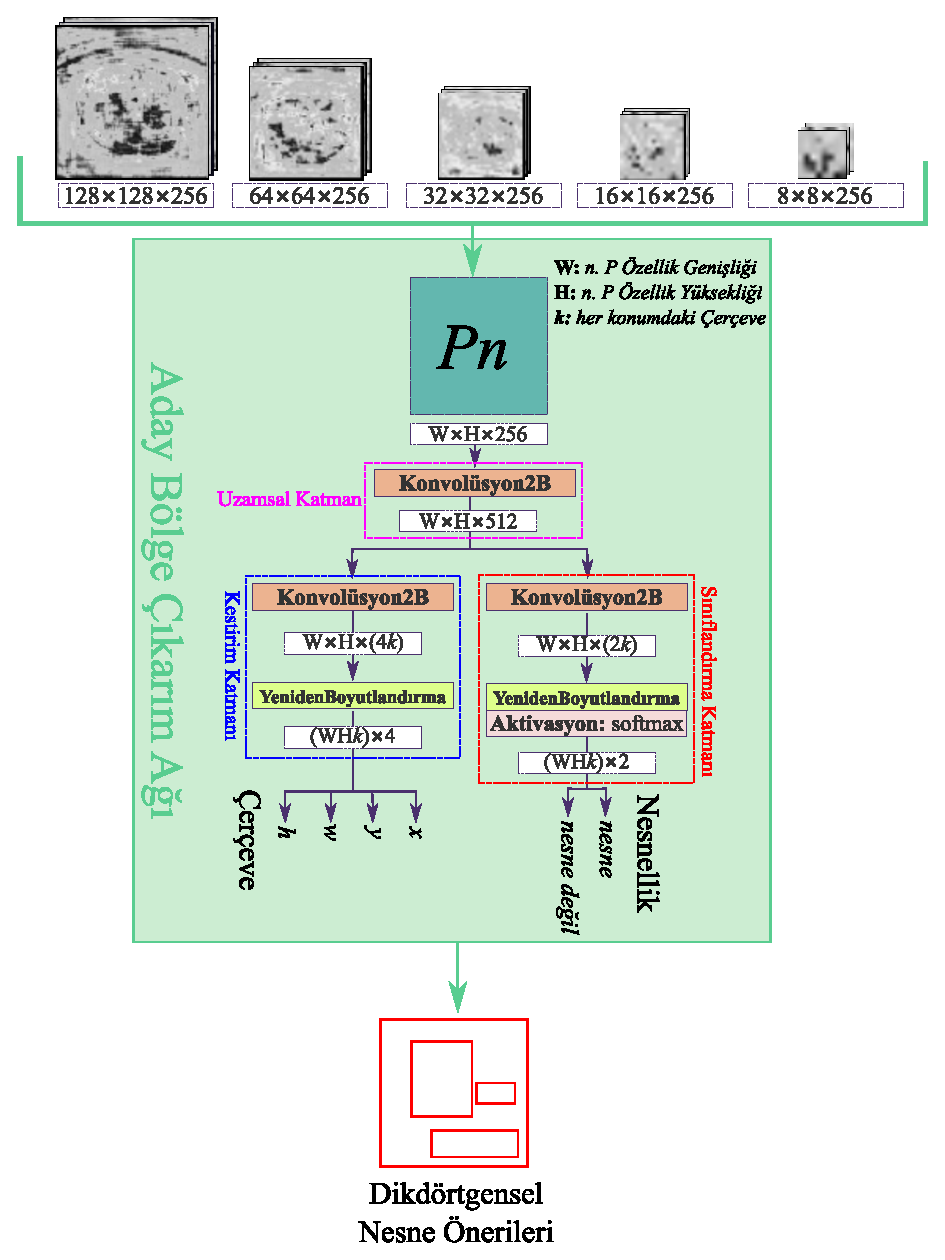
\includegraphics[scale=0.75]{Yapilan-Calismalar/Figures/region_proposal_network.pdf}
		}
	\end{center}
\end{figure}

Aday Bölge Çıkarım Ağı giriş olarak Özellik Piramit Ağı tarafından üretilen beş farklı özellik haritasını ($P2$ - $128 \times 128 \times 256$, $P3$ - $64 \times 64 \times 256$, $P4$ - $32 \times 32 \times 256$ ve $P5$ - $16 \times 16 \times 256$) almaktadır. Aday Bölge Çıkarım Ağı temelde üç farklı ana katmandan oluşmaktadır. Tasarlanan ağın ilk katmanında (Uzamsal katman - Spatial layer) piramit özellik haritaları boyutu $3 \times 3$ olan bir uzamsal filtre ile konvolüsyona tabi tutulmaktadır. Her bir piramit özellik haritası konumunda aynı anda birden çok nesne tahmini öngörülmektedir. Şekil \ref{fig:region_proposal_network}’te görülen k, piramit özellik haritasındaki her bir konum için mümkün olan maksimum öneri sayısını (anchor olarak adlandırılır) belirtmektedir. Uzamsal katmandan sonra, ilk katmanın çıkışlarına $1 \times 1$ filtre boyutuna sahip iki konvolüsyon katmanı uygulanmaktadır. Bu iki konvolüsyon katmanı regresyon ve sınıflandırıcıdır. Regresyon katmanı, k tane çerçevenin (anchor) koordinatlarını temsil eden $(WHk) \times 4$ çıkış değerine sahiptir. Bu değerler bulunan dikdörtgensel bölgenin koordinatlarını temsil etmektedir. Sınıflandırıcı katman bir softmax’ın ardından $(WHk) \times 2$ tane dikdörtgensel bölgenin nesne olup olmadığını göstermektedir.  $W \times H$ boyutuna sahip bir piramit özellik haritası için, Aday Bölge Çıkarım Ağı tarafından üretilen dikdörtgensel bölgelerin sayısı $W \times H \times k$’dır.

\paragraph{Mask R-CNN Derin Ağ Modelinin Alt Ağlarından Sınıflandırıcı Ağı'nın Yapısı}
2B BT dilimindeki pankreas bölgesinin kaba konumunu tespit etmek için bu adımda Sınıflandırıcı Ağı (Classifier Network) tasarlanmaktadır. Sınıflandırıcı Ağı'nın genel yapısı Şekil \ref{fig:classifier_network}’te verilmektedir. Sınıflandırıcı Ağı giriş olarak Aday Bölge Çıkarım Ağı tarafından üretilen dikdörtgensel nesne önerilerini ($P2$, $P3$, $P4$ ve $P5$) almaktadır. İlk olarak Piramit İlgi Bölgesi Hizalama (Pyramid ROI Align) Özellik Piramit Ağı tarafından üretilen piramit özellik haritalarını ($P2$ - $128 \times 128 \times 256$, $P3$ - $64 \times 64 \times 256$, $P4$ - $32 \times 32 \times 256$ ve $P5$ - $16 \times 16 \times 256$) Aday Bölge Çıkarım Ağı tarafından çıkarılan dikdörtgensel bölgeleri sınıflandırmaya tabi tutulabilmek için ($7 \times 7 \times 256$) çözünürlüğüne dönüştürmektedir. Daha sonra, $7 \times 7 \times 256$ çözünürlüklü her bir dikdörtgen nesne aday bölgesine $1$ konvolüsyon, $1$ paket normalizasyonu (batch normalizasyonu - BN) ve $1$ ReLU katmanları içeren blok iki kez uygulanmaktadır.  Her bir dikdörtgen nesne aday bölgesi için sabit boyutlu ($1 \times 1 \times 1024$) özellik vektörleri elde edilmektedir. Sondaki yoğun (dense) katmanlar sıkıştırılmış özellik vektörlerini girdi olarak almaktadırlar. Bu katmanlar her kaba pankreas bölgesi için sınıflandırma sonucu (pankreas ve pankreas olmayan) ve son nesne dikdörtgensel bölgesi koordinatlarını ($x,y,w,h$) gösteren çıktılar üretmektedir.

\captionsetup[figure]{margin={0.5cm,-3cm}}
\begin{figure}[h!]
	\begin{center}
		\vspace{0.4cm}
		\captionbox{Sınıflandırıcı Ağ'ın genel yapısı.\label{fig:classifier_network}}
		{
			\vspace{0.4cm}
			\includegraphics[scale=0.88]{Yapilan-Calismalar/Figures/classifier_network.pdf}
		}
	\end{center}
\end{figure}

\paragraph{Mask R-CNN Derin Ağ Modelinin Alt Ağlarından Maske Üretim Ağı'nın Yapısı}

\captionsetup[figure]{margin={0.5cm,-3cm}}
\begin{figure}[h!]
	\begin{center}
		\vspace{0.4cm}
		\captionbox{Maske Üretim Ağı'nın genel yapısı.\label{fig:mask_generation_network}}
		{
			\vspace{0.4cm}
			\includegraphics[scale=0.88]{Yapilan-Calismalar/Figures/mask_generation_network.pdf}
		}
	\end{center}
\end{figure}

2B BT diliminde algılanan pankreas bölgesinin sınırlayıcı çerçevesi içinde pankreas bölgesinin (maske) segmentasyonu için Maske Üretim Ağı (Mask Generation Network - MGN) tasarlanmaktadır. Sınıflandırıcı Ağı'ndan gelen pankreas çerçeve bölgeleri üzerinde Özellik Piramit Ağı tarafından üretilen P2, P3, P4, P5 özellik haritaları kullanılarak pankreas bölgesinin kaba sınırları tespiti hedeflenmektedir. Maske Üretim Ağı'nın genel yapısı Şekil \ref{fig:mask_generation_network}’te gösterilmektedir. Maske Üretim Ağı, Özellik Piramit Ağı tarafından üretilen özellik haritalarını ($P2$, $P3$, $P4$ ve $P5$) ve Sınıflandırıcı Ağı tarafından tahmin edilen pankreas dikdörtgensel bölgelerini girdi olarak almaktadır. İlk olarak, Piramit İlgi Bölgesi Hizalama ile girişler aynı çözünürlüğe ($14 \times 14 \times 256$) dönüştürülmektedir. Daha sonra $14 \times 14 \times 256$ çözünürlüklü her özellik haritasına $1$ konvolüsyon, $1$ paket normalizasyonu ve $1$ ReLU katmanlarını içeren blok üç kez uygulanmaktadır. Son konvolüsyon katmanı, transpoze edilen özellik haritalarını girdi olarak almaktadır. Bu katman her pankreas bölgesinin sınırlayıcı kutusunu (maskesini) gösteren bir çıktı oluşturmaktadır.

\subsubsection{Kaba Pankreas Bölgesinin Mask R-CNN'den Elde Edilen Merkez Bilgisi ile Belirlenmesi}

\captionsetup[figure]{margin={0.3cm,-3cm}}
\begin{figure}[h!]
	\begin{center}
		\vspace{0.4cm}
		\captionbox{Kaba Pankreas Bölgesi Çıkarılması aşamasının şematik temsili.\label{fig:center_of_mass}}
		{
			\vspace{0.4cm}
			\includegraphics[scale=0.61]{Yapilan-Calismalar/Figures/center_of_mass.pdf}
		}
	\end{center}
\end{figure} 

Pankreas İlgi Bölgesinin Belirlenmesi fazının ikinci aşaması olan Kaba Pankreas Bölgesinin Çıkarılması, Belirlenen İlgi Bölgesinde Pankreas Segmentasyonu fazı için işlenen BT dilimlerinin boyutunu azaltmayı amaçlamaktadır. Kaba Pankreas Bölgesinin Çıkarılması aşaması, ilk aşamada Mask R-CNN modeli ile üretilen kaba pankreas bölgelerini giriş olarak almaktadır. Şekil \ref{fig:center_of_mass}’da Kaba Pankreas Bölgesinin Çıkarılması aşamasının şematik temsili verilmektedir. Şekil \ref{fig:center_of_mass}’da gösterildiği gibi, ilk olarak maskelenmiş 2B BT dilimleri ($512 \times 512 \times N$) üzerindeki pankreas bölgesinin merkezi Eşitlik \ref{eq:centerofmass} ile hesaplanmaktadır.
\begin{equation}
	\label{eq:centerofmass}
	\left(x_{c}, y_{c}, z_{c}\right)=\frac{1}{N} \sum_{i=1}^{N}\left(x_{i}, y_{i}, z_{i}\right)
\end{equation}

Eşitlik \ref{eq:centerofmass}’de $\left(x_{c}, y_{c}, z_{c}\right)$ kaba pankreas bölgesinin merkezini, $\left(x_{i}, y_{i}, z_{i}\right)$ kaba pankreas bölgesindeki noktaların koordinatlarını ve N kaba pankreas bölgesindeki noktaların sayısını temsil etmektedir. Kaba pankreas bölge merkezinin hesaplanmasından sonra, her bir BT dilimindeki ($512 \times 512$) 3B kümeden elde edilen kaba merkezin etrafındaki bölge kırpılarak 2B alt BT dilimleri ($256 \times 256 \times 2N / 3$) çıkarılmaktadır. Bu bölge, x ve y eksenlerinin sol ve sağ yönlerinde 128 piksel ve z ekseninin alt ve üst yönlerinde 2N/6 dilimlerinin hareket ettirilmesiyle oluşturulmaktadır; burada x, y, z, kaba pankreas bölgesinin 3B merkez koordinatlarını, $N$ BT dilimlerinin sayısını göstermektedir.

\subsection{Belirlenen İlgi Bölgesinde Pankreas Segmentasyonu}
Mask R-CNN modeli, nesne kaba hatlarını bulmak için oldukça uygun bir algoritmadır. Fakat hatlarının çok değişken olduğu nesnelerin sınır tespiti için yeterince başarılı olamamaktadır. Bunun en temel sebebi nihai maskeleme aşamasında hesaplama yükünü azaltmak için tüm aday bölgelerin $14 \times 14$ çözünürlüğüne düşürülmesidir. Bu nedenle Mask R-CNN modeli nesnenin kaba hatlarını çıkarmada oldukça başarılı olsa da nesne sınırlarının daha doğru belirlenebilmesi için daha detaylı bir yaklaşım gerekmektedir.

Önerilen çalışmada giriş olarak verilen 2B BT dilimlerinin ($512 \times 512 \times N$) tümünü işlemek yerine, ikinci faz (Belirlenen İlgi Bölgesinde Pankreas Segmentasyonu) aday pankreas bölgesini kapsayan 2B alt BT dilimlerini ($256 \times 256 \times 2N/3$) kullanmaktadır. Bu sayede, daha tatmin edici sonuçlar elde edilmekte, otomatik pankreas segmentasyonu için hesaplama karmaşıklığı ve maliyeti azaltılmaktadır. Bu faz, 3B U-Net modelini kullanarak aday pankreas bölgesini içeren 2B alt BT dilimleri tekrar düzenlemeyi amaçlamaktadır. Tasarlanan modelde, önceki fazda (Pankreas İlgi Bölgesinin Belirlenmesi) üretilen 2B alt BT dilimleri ($256 \times 256 \times 2N/3$) giriş olarak alınmaktadır. Pankreas bölgesinin segmente edilmiş 2B alt BT dilimleri ($256 \times 256 \times 2N/3$) çıkış olarak üretilmektedir. Pankreas Segmentasyon fazı ön işlem (pre - processing), 3B U-Net, son işlem (post-processing) ve geri montajlama (decropping) olmak üzere dört adımdan oluşmaktadır. Şekil \ref{fig:3dunet1} Pankreas Segmentasyon fazında kullanılan 3B U-Net modelinin şematik temsilini göstermektedir. Bu model, kodlayıcı (Şekil \ref{fig:3dunet1}'de aşağı yönlü sol taraf) ve kod çözücü (Şekil \ref{fig:3dunet1}'de yukarı yönlü sağ taraf) olmak üzere iki temel aşamadan oluşmaktadır. Pankreas Segmentasyonu fazında uygulanan bu adımların detayları bundan sonraki alt başlıklarda daha ayrıntılı verilecektir. 

\captionsetup[figure]{margin={0.4cm,-2cm}}
\begin{figure}[h!]
	\begin{center}
		\vspace{0.4cm}
		\captionbox{Pankreas Segmentasyon fazında kullanılan 3B U-Net modelinin şematik temsili. \label{fig:3dunet1}}
		{
			\vspace{0.4cm}
			\includegraphics[scale=0.6]{Yapilan-Calismalar/Figures/3dunet.pdf}
		}
	\end{center}
\end{figure} 

\subsubsection{Pankreas Segmentasyonu İçin Ön İşlem}
Belirlenen İlgi Bölgesinde Pankreas Segmentasyonu fazında 3B U-Net modelini uygularken GPU bellek tüketimini azaltmak için önceki fazda (Pankreas İlgi Bölgesinin Belirlenmesi) oluşturulan 2B alt BT dilimlerinin boyutu ($256 \times 256 \times 2N/3$) yerine ($64 \times 64 \times 2N/3$) olarak yeniden boyutlandırılmaktadır.

\subsubsection{Pankreas Segmentasyonunun 3B U-Net Modeli ile Gerçekleştirilmesi}
3B U-Net modeli, kodlayıcı ve kod çözücü olmak üzere iki temel aşamadan oluşmaktadır. Bu iki temel aşama şu şekilde açıklanabilmektedir:

\paragraph{3B U-Net Modeli Kodlayıcı Aşaması}
Kodlayıcı aşamasının temel amacı, aday pankreas bölgesinden küresel karakteristikleri çıkarmaktır. Bu aşama, bir önceki fazda üretilen pankreasın kaba olarak segmente edilmiş 2B alt BT dilimlerinin ($256 \times 256 \times 2N / 3$) işlem yükünü azaltmak için yeniden boyutlandırılmış versiyonu olan 2B alt BT dilimlerini ($64 \times 64 \times 2N / 3$) giriş veri seti olarak almaktadır. Tasarlanan modelde, 1 konvolüsyon, 1 paket normalizasyon, 1 ReLU aktivasyon ve 1 maksimum havuzlama katmanlarını içeren üç bölüm bulunmaktadır. Bu üç bölümden önce, ($64 \times 64 \times 2N / 3$) boyutundaki giriş katmanına ($1, 4, 4$) çekirdek boyutlu 1 konvolüsyon, 1 paket normalizasyonu ve 1 ReLU aktivasyon işlemleri uygulanmaktadır. Literatür çalışmalarında küçük boyutlu konvolüsyon filtrelerinin daha iyi performans sağladığı gösterilmektedir. Bu nedenle, bu modelin tüm bölümlerindeki konvolüsyon katmanlarının 3B filtre büyüklükleri $3 \times 3 \times 3$ olarak alınmaktadır. Konvolüsyon katmanından sonra çıkış değerleri paket normalizasyonu katmanıyla normalleştirilmektedir. Eğitimi hızlandırmak ve eğrilik geri yayılımını sağlamak için katmanlarda ReLU aktivasyonu uygulanmaktadır. Tüm bölümlerin sonunda, maksimum havuzlama katmanı tasarlanan modelin hesaplama ve karmaşıklık maliyetlerini azaltmak için önceki katmanlarda üretilen çıktıları alt örneklemektedir. İlk bloktaki maksimum havuzlama katmanının filtre boyutu ($2 \times 2 \times 2$), diğer bloklardaki maksimum havuzlama katmanlarının filtre boyutundan ($1 \times 2 \times 2$) farklıdır. Buradaki amaç 3B maksimum havuzlama filtresinin ilk elemanının 3B BT görüntüsündeki dilim sayısına etki etmesidir. Bu değerin ilk blokta $2$ olması BT görüntülerinin dilim sayısı ve hesaplama maliyetini düşürmektedir. Fakat diğer bloklarda bu sayı $1$ değerine sabitlenerek 3B uzayda dilim sayısı azaltılmakta ve maskeleme sonucunun bozulmasının önüne geçilmektedir.

\paragraph{3B U-Net Modeli Kod Çözücü Aşaması}
3B U-Net modeli Kod Çözücü aşaması, Kodlayıcı aşamasında öğrenilen özellikleri kullanarak ($64 \times 64 \times 2N / 3$) boyutuna sahip pankreas segmentasyon sonuçlarını oluşturmaktadır. Tasarlanan modelde $1$ paket normalizasyonu, 1 ReLU, 1 ters konvolüsyon ve 1 birleştirme katmanlarını içeren üç bölüm bulunmaktadır. Konvolüsyon katmanının aksine, ters konvolüsyon katmanları küresel karakteristiklerin boyutunu arttırmaktadır. Tüm bölümlerdeki ters konvolüsyon katmanlarının filtre boyutları $3 \times 3 \times 3$ olarak atanmaktadır. Ters konvolüsyon katmanından sonra, atlama bağlantıları ile birleştirme işlemi kodlayıcı aşamasından yüksek çözünürlüklü global özellikler sağlamaktadır. Tüm bölümlerin sonundaki konvolüsyon, kırpma ve sıfır dolgulama katmanları segmente edilmiş pankreas bölgelerini üretmektedirler. Şekil \ref{fig:3dunet1}'de gösterildiği gibi, son konvolüsyon katmanının aktivasyon fonksiyonu olarak Sigmoid aktivasyon fonksiyonu kullanılmaktadır. Sigmoid aktivasyon fonksiyonu 0 ile 1 arasında çıktılar üretmektedir. Ek olarak, ikili çapraz entropi (binary cross-entropy) kayıp fonksiyonu olarak kullanılmaktadır. Bu sayede önerilen model piksel değerleri $0$ ile $1$ arasında değişen $2N/3$ adet $64 \times 64$ görüntü üretmektedir.

\subsubsection{Pankreas Segmentasyonu İçin Son-işlem (Post - processing)}
Önceki adımda 3B U-Net modeli ile oluşturulan $2N/3$ adet $64 \times 64$ boyutuna sahip görüntü, piksel değerleri $0$ ile $1$ arasında olan olasılık haritalarını temsil etmektedir. Bu adımda, olasılık haritalarında pankreas veya pankreas dışı bölgenin belirlenmesi için öncelikle Sert Eşikleme (Hard Thresholding) işlemi uygulanmaktadır. Bu işlem için eşik değeri $0,5$ olarak kabul edilmektedir. Bu nedenle $0,5$'ten büyük piksel değerleri pankreas bölgesini ($1$) belirtirken, diğer değerler pankreas dışı bölgeler ($0$) olarak kabul edilmektedir. Daha sonra pankreas veya pankreas dışı bölgeyi ($64 \times 64 \times 2N/3$) gösteren bu ikili sonuçlar ($256 \times 256 \times 2N/3$) olarak yeniden boyutlandırılmaktadır.

\subsubsection{Belirlenen Kaba İlgi Bölgesinde Gerçekleştirilen Hassas Segmentasyon Sonucunun Geri Montajlanması}
Son işleme adımında oluşturulan 2B alt BT dilimleri ($256 \times 256 \times 2N/3$), ikinci aşamada oluşturulan temel konum bilgisi kullanılarak sıfır doldurulmuş 2B alt BT dilimlerine ($512 \times 512 \times N$) geri montajlanmaktadır.


%********************** Pankreas ve Pankreas Tümörü
\section{Pankreas ve Pankreas Tümörü Segmentasyonu İçin Önerilen İki Fazlı Yöntemin Farklı Derin Öğrenme Teknikleri ile İncelenmesi}

Bu tez çalışmasının ilk kısmında bölüm \ref{sec:pancreas}'de  bahsedilen pankreas segmentasyonu için iki fazlı yöntem önerilmektedir. Önerilen bu yöntemin fazları Pankreas İlgi Bölgesinin Belirlenmesi ve Belirlenen İlgi Bölgesinde Pankreas Segmentasyonu'dur. Bu bölümde önerilen iki fazlı yöntem kullanılarak pankreas, pankreas tümörü ve diğer dokular olmak üzere 3 sınıflı segmentasyon gerçekleştirmektedir. Bu kapsamda öncelikle pankreas kaba bölgesinin belirlenmesi için gerçekleştirilen iyileştirmeler ele alınmakta ve farklı derin öğrenme modelleri ile pankreas kaba bölgesinin belirlenmesine yönelik sonuçlar alınmaktadır. Belirlenen kaba pankreas alt BT bölgesinde pankreasın hassas segmentasyonu için bölüm \ref{sec:pancreas}'de 3B UNet yöntemi kullanılmaktadır. Tez çalışmasının bu kısmında kaba pankreas bölgesinde gerçekleştirilecek iyileştirmeleri irdelemek amacı ile öncelikle standart 3B FCN Oto Kodlayıcı yöntemi kullanılarak hassas segmentasyon gerçekleştirilmekte ve sonuçlar alınmaktadır. Daha sonra 3B UNet modeli 3 sınıflı segmentasyona uygun hale getirilmekte ve ara katmanlarda gerçekleştirilen bazı iyileştirmeler ile sonuçlar incelenmektedir. Son olarak hassas pankreas segmentasyonu aşaması için 3B UNet++ yöntemi  kullanılarak segmentasyon gerçekleştirilmektedir. 

\subsection{İlgi Bölgesinin Belirlenmesi Aşamasında Kullanılan İyileştirme Yöntemleri}

İlgi Bölgesinin Belirlenmesi aşaması 3B verilerin bilgisayar belleğinde fazla yer kaplamasından ve bu verilerden bilgi çıkarımı yapılmak istendiğinde kullanılan yöntemlerin hesaplama maliyetlerinin yüksek olmasından dolayı önemli bir aşama olarak karşımıza çıkmaktadır. Bu çalışmanın ilk kısmında kaba olarak pankreas bölgesini belirlemek için Mask R-CNN yöntemi kullanılmaktadır. Benzer şekilde tez çalışmasının ikinci aşamasında pankreas ve pankreas tümörü dokularının hassas segmentasyonu amacı ile de öncelikle pankreas ilgi bölgesinin tespit edilmesi gerçekleştirilmektedir. İlgi Bölgesinin Belirlenmesi aşamasında Mask R-CNN modeli için farklı özellik çıkarıcılar kullanılmakta ve performans karşılaştırılması yapılmaktadır. 

\captionsetup[figure]{margin={0.4cm,0cm}}
\begin{figure}[h!]
	\begin{center}
		\vspace{0.4cm}
		\captionbox{ResNet 50 ve ResNet 101 özellik çıkarıcıları kullanan Mask R-CNN modelinin şematik temsili. \label{fig:head_network2}}
		{
			\vspace{0.4cm}
			\includegraphics[scale=0.6]{Yapilan-Calismalar/Figures/head_network2.pdf}
		}
	\end{center}
\end{figure} 

Mask R-CNN modeli Şekil \ref{fig:maskrcnn}'da gösterildiği gibi Çekirdek Ağı, Özellik Piramit Ağı, Aday Bölge Çıkarım Ağı, Sınıflandırıcı Ağı ve Maske Üretim Ağı olmak üzere beş ana adımdan oluşmaktadır. Bu alt ağlardan biri olan Çekirdek Ağı kısmında pankreas organı için belirleyici özellik haritalarının üretilmesi gerçekleştirilmektedir. Diğer tüm alt ağlar ise bu özellik haritalarından elde edilen ön bilgi ile çalışmaktadır. Bu sebeple Mask R-CNN modelinin başarısını en fazla etkileyen alt adım olarak Çekirdek Ağı karşımıza çıkmaktadır. Literatürde CNN tabanlı farklı özellik çıkarıcılar kullanılarak Mask R-CNN modelinin performansındaki değişiklikleri incelemek mümkündür.


ResNet 50 ve ResNet 101 özellik çıkarıcıları kullanan Mask R-CNN modelinin şematik temsili Şekil \ref{fig:head_network2}'de verilmektedir. Şekil \ref{fig:head_network2}'de Çekirdek Ağı olarak ResNet-50 ve ResNet-101 CNN özellik çıkarıcıları kullanılması durumunda üretilen C1, C2, C3, C4 ve C5 çıkışları görülmektedir. Bir sonraki Özellik Piramit Ağı adımı üretilen C2, C3, C4 ve C5 çıkışları ile $1 \times 1$ konvolüsyon filtreleri kullanarak derinlikli konvolüsyonlama (depthwise convolution) işlemi gerçekleştirdiği için Çekirdek Ağı adımında üretilen çıkışların C2 ($128 \times 128 \times n$), C3 ($64 \times 64 \times n$), C4 ($32 \times 32 \times n$) ve C5 ($16 \times 16 \times n$) özellik haritalarının sayısını belirten $n$ değeri önemsizleşmektedir. C2, C3, C4 ve C5 çıkışlarından gelen özellik haritaları Özellik Piramit Ağı adımında kullanılarak P2 ($128 \times 128 \times 256$), P3 ($64 \times 64 \times 256$), P4 ($32 \times 32 \times 256$), P5 ($16 \times 16 \times 256$) ve P5 ($8\times 8 \times 256$) çıkışları üretilmektedir. Çekirdek Ağı'nın özellik çıkarıcı CNN modeli olarak $n$ ilgili katmandaki özellik haritası sayısını belirtmek üzere C2 ($128 \times 128 \times n$), C3 ($64 \times 64 \times n$), C4 ($32 \times 32 \times n$) ve C5 ($16 \times 16 \times n$) özellik haritalarını üretebilecek herhangi bir modelin kullanılması Mask R-CNN çalışmasını etkilememektedir. Bu sayede farklı çekirdek ağlar ile Mask R-CNN yönteminin kullanıldığı pankreas kaba bölgesinin tespiti gerçekleştirilebilmektedir.

Bu tez çalışmasında pankreas ve pankreas tümör segmentasyonu için 3 farklı model (3B Standart FCN Oto Kodlayıcı, 3B UNet ve 3B UNet++) performansları ayrı ayrı kullanılmaktadır.
Pankreas ve pankreas tümör segmentasyonu tek başına 2 sınıflı (diğer dokular, pankreas) pankreas segmentasyonundan farklı olarak 3 sınıflı (diğer dokular, pankreas, pankreas tümörü) bir segmentasyon problemidir.

3 sınıflı segmentasyon gerçekleştirilecek verilerde Pankreas İlgi Bölgesinin Belirlenmesi aşaması ile bölgenin küçültülmüş olmasına karşın hala sınıflar arasında dengeli bir voksel dağılımı mevcut değildir. Tümör dokuları bazı hastalarda pankreas ve diğer dokulara nazaran oldukça büyük yer tutmaktadır. Dengelenmemiş veriseti (imbalanced dataset) olarak adlandırılan bu probleme çözüm üretecek şekilde önerilen yöntemin ikinci aşaması olan hassas segmentasyon aşamasının güncellenmesi gerekmektedir. Dengelenmemiş veriseti probleminin önüne geçebilmek için CCE kayıp fonksiyonunun $\alpha$ ve $\gamma$ hiper parametreleri eklenerek özelleştirilmiş bir versiyonu olan FL kayıp fonksiyonu tercih edilmektedir. Ayrıca 3 modelde de (3B Standart FCN Oto Kodlayıcı, 3B UNet ve 3B UNet++) son katmanın aktivasyon fonksiyonu olarak softmax aktivasyon fonksiyonu kullanılmaktadır. CCE kayıp fonksiyonu türevi olan tüm kayıp fonksiyonlarında CCE kayıp fonksiyonunda olduğu gibi son katman aktivasyon fonksiyonu olarak softmax aktivasyon fonksiyonu tercih edilmektedir. Böylece girişten uygulanan herbir hastaya ait volümetrik BT verisinden 3 farklı (diğer dokular, pankreas, pankreas tümörü) sınıfı temsilen volümetrik maske verileri üretilmektedir.

\subsection{Belirlenen İlgi Bölgesinde Pankreas ve Pankreas Tümör Segmentasyonu Gerçekleştirmek Amacıyla Denenen Farklı Derin Ağ Modelleri}

BU tez çalışmasında volumetrik BT görüntülerinde pankreas ve pankreas tümör segmentasyonu gerçekleştirmek için 3 farklı derin ağ segmentasyon modeli kullanılmıştır. BU modeller sırasıyla 3B FCN Oto Kodlayıcı modeli, 3B UNet modeli ve 3B UNet++ modelidir. 

\subsubsection{3B FCN Oto Kodlayıcı Modeli ile Pankreas ve Pankreas Tümör Segmentasyonu}
Oto kodlayıcılar çeşitli amaçlar için kullanılabilmekle birlikte segmentasyon problemlerinde de sıklıkla tercih edilmektedir. Bu tez çalışmasında kullanılan 3B oto kodlayıcı modeli standart oto kodlayıcılara uygun şekilde ele alınmakta ve 3 sınıflı (diğer dokular, pankreas, pankreas tümörü) probleme uygun şekilde yeniden dizayn edilmektedir. Pankreas ve Pankreas Tümörü Segmentasyonunda kullanılan 3B FCN Oto Kodlayıcı'nın şematik temsili Şekil \ref{fig:3dotokod}'da verilmektedir. Standart bir oto kodlayıcı temelde kodlama ve kod çözme aşamasından oluşmaktadır. Girişten uygulanan veri ardışık konvolüsyon katmanları ile kodlanmakta yani manuel olarak işaretlenmiş volümetrik maske verileri kullanılarak volümetrik BT verilerinin özellik haritaları çıkarılmaktadır. Pankreas İlgi Bölgesinin Belirlenmesi aşaması ile $192 \times 256 \times 256$ ölçeklerine indirgenen volümetrik giriş verisi ardışık konvolüsyon işlemine tabi tutularak kodlama aşamasında $3 \times 4 \times 4$ ölçeklerine kadar indirgenerek kodlama işlemi gerçekleştirilmektedir. Daha sonra çıkarılan bu özellik haritalarına ardışık ters konvolüsyon katmanları ile kod çözme işlemi gerçekleştirilmekte yani öğrenilen özellik haritalarından tahmin maskesi volümetrik verileri inşa edilmektedir. Bu aşamada $3 \times 4 \times 4$ ölçeklerine indirgenmiş özellik haritaları ardışık ters konvolüsyon işlemlerinin ardından $96 \times 128 \times 128$ ölçeklerine çıkarılmaktadır. Daha sonra tekrar bir ters konvolüsyon işlemi softmax aktivasyon fonksiyonu ile kullanılarak 3 adet $192 \times 256 \times 256$ ölçeklerinde tahmin maskeleri üretilmektedir.  

\captionsetup[figure]{margin={0.4cm,-1.5cm}}
\begin{figure}[h!]
	\begin{center}
		\vspace{0.4cm}
		\captionbox{Pankreas ve Pankreas Tümörü Segmentasyonunda kullanılan 3B FCN Oto Kodlayıcı'nın şematik temsili.\label{fig:3dotokod}}
		{
			\vspace{0.4cm}
			\includegraphics[scale=0.6]{Yapilan-Calismalar/Figures/3dfcn.pdf}
		}
	\end{center}
\end{figure} 

Üretilen tahmin maskeleri sırası ile diğer dokular, pankreas ve pankreas tümörünü temsil eden volümetrik verilerdir. Aslında üretilen bu 3 farklı volümetrik maske verisinde her bir voksel için softmax aktivasyon fonksiyonu ile 3 sınıfı temsilen 3 farklı çıkış üretilmektedir. Yani voksel ölçeğinde bir sınıflandırma işlemi gerçekleştirilerek segmentasyon yapılmaktadır.

Bu tez çalışmasında öncelikle 3B Standart FCN Oto Kodlayıcı modelini tercih etmekteki amaç 3B U-Net yaklaşımındaki atlama bağlantılarının (skip conections) segmentasyona etkilerinin incelenmesidir. Standart FCN Oto Kodlayıcı modellerinin atlama bağlantıları eklenerek özelleştirilmiş versiyonu olan U-Net yaklaşımı ardışık konvolüsyon katmanlarında derinlik arttıkca kaybedilen özelliklerin geri kazanımını hedeflemektedir.

\subsubsection{3B U-Net Modeli ile Pankreas ve Pankreas Tümör Segmentasyonu}
Oto kodlayıcıların atlama bağlantıları (skip connections) eklenerek güçlendirilmiş versiyonu olan U-Net yaklaşımı ardışık konvolüsyon katmanlarında yaşanan bilgi kaybının önüne geçmeyi amaçlamaktadır. Pankreas ve Pankreas Tümörü Segmentasyonunda kullanılan 3B U-Net modelinin şematik temsili Şekil \ref{fig:3dunet2}'da verilmektedir. Oto kodlayıcılarda olduğu gibi 3B U-Net modeli de girişinden girdi olarak aldığı volümetrik verilerde ardışık konvolüsyon işlemi gerçekleştirerek kodlama işlemi gerçekleştirmekte ve daha sonra giriş verisinden elde edilen özellik haritaları üzerinde ters konvolüsyon katmanları ile ters yönde kod çözme işlemi gerçekleştirmektedir.

\captionsetup[figure]{margin={0.4cm,-1.5cm}}
\begin{figure}[h!]
	\begin{center}
		\vspace{0.4cm}
		\captionbox{Pankreas ve Pankreas Tümörü Segmentasyonunda kullanılan 3B U-Net modelinin şematik temsili.\label{fig:3dunet2}}
		{
			\vspace{0.4cm}
			\includegraphics[scale=0.6]{Yapilan-Calismalar/Figures/3dunet2.pdf}
		}
	\end{center}
\end{figure} 

Bu tez çalışmasında pankreas segmentasyonu için önerilen yöntemin segmentasyon aşamasında kullanılan 3B U-Net modelinden farklı olarak pankreas ve pankreas kanser dokularının segmentasyonu için geliştirilen 3B U-Net modelinde üç sınıflı(diğer dokular, pankreas, pankreas tümörü) segmentasyon gerçekleştirebilen bir model üretilmektedir. Böylece standart oto kodlayıcılardan farklı olarak eklenen atlama bağlantılarının segmentasyona etkileri incelenmektedir. Şekil \ref{fig:3dunet2}'da detayları gösterilen 3D U-Net modelinde girişinden Pankreas İlgi Bölgesinin Belirlenmesi aşaması ile küçültülmüş $192 \times 256 \times 256$ ölçeklerinde volümetrik BT alt görüntüleri uygulanmaktadır. Bu veriler ardışık konvolüsyon katmanları ile küçültülerek (kodlama) sırasıyla $96 \times 128 \times 128$, $48 \times 64 \times 64$, $24 \times 32 \times 32$, $12 \times 16 \times 16$, $6 \times 8 \times 8$ ve $3 \times 4 \times 4$ ölçeklerine indirgenmektedir. Bu özellik haritaları ters konvolüsyon işlemleri ile ters yönde ölçek artımına tabi tutulmaktadır. Ters konvolüsyon sonucu ölçeği büyütülen özellik haritaları kodlama aşamasından gelen eşit ölçekli özellik haritaları ile birleştirilmektedir. Ters yönde (kod çözme) $96 \times 128 \times 128$ ölçeğine gelindiğinde son bir ters konvolüsyon işlemi softmax aktivasyon fonksiyonu ile kullanılarak 3 adet $192 \times 256 \times 256$ ölçeklerinde tahmin maskeleri üretilmektedir. Bu tahmin maskeleri sırası ile diğer dokular, pankreas ve pankreas tümörünü temsil eden volümetrik verilerdir. Aslında üretilen bu 3 farklı volümetrik maske verisinde herbir voksel için softmax aktivasyon fonksiyonu ile 3 sınıfı temsilen 3 farklı çıkış üretilmektedir. Yani voksel ölçeğinde bir sınıflandırma işlemi gerçekleştirilerek segmentasyon yapılmaktadır.  


\subsubsection{3B U-Net++ Modeli ile Pankreas ve Pankreas Tümör Segmentasyonu}
3B U-Net modelinde atlama bağlantılarının önemi irdelenirken 3B U-Net++ modelinde daha karmaşık atlama bağlantıları ile bir anlamda iç içe U-Net modellerinin performansa etkileri irdelenmektedir. U-Net++ yaklaşımı atlama bağlantılarının çok daha kompleks kullanıldığı bir model olarak karşımıza çıkmaktadır. Pankreas ve Pankreas Tümörü Segmentasyonunda kullanılan 3B U-Net++  modelinin şematik temsili Şekil \ref{fig:3dunet++}'de verilmektedir. 

\captionsetup[figure]{margin={0.4cm, 0.2cm}}
\begin{figure}[h!]
	\begin{center}
		\vspace{0.4cm}
		\captionbox{Pankreas ve Pankreas Tümörü Segmentasyonunda kullanılan 3B UNet++ modelinin şematik temsili.\label{fig:3dunet++}}
		{
			\vspace{0.4cm}
			\includegraphics[scale=0.45]{Yapilan-Calismalar/Figures/3dunet++.pdf}
		}
	\end{center}
\end{figure} 

3B U-Net++ yönteminde atlama bağlantılarının çokluğundan kaynaklı hesaplama maliyetini düşürmek adına kodlama aşamasında ölçek azaltma işleminde konvolüsyon katmanları yerine maksimum havuzlama katmanları ile gerçekleştirilmektedir. Konvolüsyon katmanlarında özellik haritalarının ölçekleri dolgulama ile korunmaktadır.

3B U-Net++ modeli temelde iç içe U-Net modellerinden oluşmaktadır. U-Net++ modelinin girişinden Pankreas İlgi Bölgesinin Belirlenmesi aşaması ile küçültülmüş $192 \times 256 \times 256$ ölçeklerinde volümetrik BT alt görüntüleri uygulanmaktadır. Sırası ile $X^{0,0}$,$X^{1,0}$ ve $X^{0,1}$ blokları en küçük U-Net alt ağını temsil etmektedir. İkinci seviyeden U-Net modeli sırasıyla $X^{0,0}$, $X^{1,0}$, $X^{2,0}$, $X^{1,1}$ ve $X^{2,0}$ blokları ile temsil edilmektedir. Üçüncü seviyeden U-Net modeli sırasıyla $X^{0,0}$, $X^{1,0}$, $X^{2,0}$, $X^{3,0}$, $X^{2,1}$, $X^{1,2}$ ve $X^{0,3}$ blokları ile temsil edilmektedir. Son olarak dördüncü U-Net modeli sırasıyla $X^{0,0}$, $X^{1,0}$, $X^{2,0}$, $X^{3,0}$, $X^{4,0}$, $X^{3,1}$, $X^{2,2}$, $X^{1,3}$ ve $X^{0,4}$ blokları ile temsil edilmektedir. Görüldüğü gibi U-Net++ yöntemi iç içe U-Net modellerinden oluşmaktadır. Modelin $X^{4,0}$ blok çıkışı $96 \times 128 \times 128$ ölçeğinde veri üretmekte ve bu veri son bir ters konvolüsyon işlemine tabi tutulmaktadır. Konvolüsyon işleminin çıkışı softmax aktivasyon fonksiyonuna tabi tutularak 3 adet $192 \times 256 \times 256$ ölçeklerinde tahmin maskeleri üretilmektedir. Bu tahmin maskeleri sırası ile diğer dokular, pankreas ve pankreas tümörünü temsil eden volümetrik verilerdir. Aslında üretilen bu 3 farklı volümetrik maske verisinde her bir voksel için softmax aktivasyon fonksiyonu ile 3 sınıfı temsilen 3 farklı çıkış üretilmektedir. Yani voksel ölçeğinde bir sınıflandırma işlemi gerçekleştirilerek segmentasyon yapılmaktadır.
\chapter{BULGULAR VE İRDELEME \label{sec:YapilanCalismalar}}

Tez çalışmasında önerilen yaklaşımlar, pankreas hastalıkları bulunan kişilerin sağkalım oranını artırmak, tanı, tedavi ve cerrahide tıp doktorlarına yardımcı olmak için pankreas ve pankreas tümörü segmentasyonu gerçekleştirmektedirler. Tez çalışmasının bu bölümünde ilk olarak önerilen yaklaşımların gerçekleştirildiği cihaz konfigürasyonu hakkında bilgiler verilecektir. Daha sonra çalışma kapsamında önerilen yaklaşımların abdominal kontrastlı pankreas BT dilimleri üzerinde gerçekleştirilen deneyleri, elde edilen görsel ve sayısal sonuçları irdelenecektir. Gerçekleştirilen tez çalışması pankreas ve pankreas tümörü segmentasyonu olmak üzere iki kısımdan oluşmaktadır. Bu iki kısım için elde edilen bulgular ve önerilen yaklaşımların literatürdeki çalışmalarla kıyaslanmaları ilgili ana başlıklar altında ayrı ayrı verilecektir.
 
Tez çalışmasında birinci kısım olan Pankreas Segmentasyonu için NIH veri seti, ikinci kısım olan Pankreas ve Pankreas Tümörü Segmentasyonu için MSD veri seti kullanılmaktadır. Çalışmada önerilen yaklaşımların analizi için kullanılan veri setlerinin ayrıntılı açıklamaları Bölüm \ref{sec:genel}’de ilgili alt başlıklar altında verilmektedir. Dolayısıyla bu bölümde tekrar veri seti analizi yapılmayacaktır. 

\section{Cihaz Konfigürasyonu}
Pankreas segmentasyonunun gerçekleştirildiği tez çalışmasının ilk kısmını Pankreas İlgi Bölgesinin Belirlenmesi ve Belirlenen İlgi Bölgesinde Pankreas Segmentasyonu fazları oluşturmaktadır. Pankreas ve pankreas tümörü segmentasyonunun gerçekleştirildiği ikinci kısım ise Pankreas İlgi Bölgesinin Belirlenmesi, Belirlenen İlgi Bölgesinde Pankreas ve Pankreas Tümörü Segmentasyonu fazlarından oluşmaktadır. 

Tez çalışmasının ilk kısmı Intel Core i7-9750 2.60 GHz işlemci, 32 GB RAM ve NVIDIA GeForce RTX 2060 GPU 6GB VRAM 1920 CUDA çekirdeği bulunan bir bilgisayarda çalışan Pyton 3.6 yazılımı ile arka planda Tensorflow kütüphanesini kullanan Keras kütüphanesi temelli bir cihaz yapılandırması kurularak gerçekleştirilmiştir. Bu kısımda kaynak tüketimi az yüksek doğruluklu pakreas segmentasyonu gerçekleştiren bir yöntem önerilmiştir.

Tez çalışmasının ikinci kısmı AMD Ryzen 7 3800x 3.90 GHz işlemci, 32 GB RAM ve NVIDIA GeForce RTX 3060 GPU 12GBVRAM 3584 CUDA çekirdeği bulunan bir bilgisayarda çalışan Pyton 3.6 yazılımı ile arka planda Tensorflow kütüphanesini kullanan Keras kütüphanesi temelli bir cihaz yapılandırması kurularak gerçekleştirilmiştir. Bu kısımda ilk kısımda önerilen yöntem pankreas ve pankreas tümör segmentasyonu gerçekleştirebilmek amacı ile tekrar ele alınmış ve farklı derin öğrenme teknikleri ile zenginleştirilmiştir.

\section{Pankreas İlgi Bölgesinin Belirlenmesi ve İlgi Bölgesinde Pankreas Segmentasyonu ile Elde Edilen Deneysel Sonuçlar}

\subsection{Önerilen Ağ Mimarilerinin Özellikleri}
Pankreas Segmentasyonu için önerilen iki aşamalı yöntemin ilk fazı olan Pankreas İlgi Bölgesinin Belirlenmesi'nde Waleed Abdulla tarafından geliştirilen Keras ve Tensorflow tabanlı Mask R-CNN modeli \cite{he2017mask} ResNet-101 çekirdek ağı ile kullanılmaktadır. Bu model orijinal olarak renkli görüntülerin segmentasyonu için kullanılmaktadır. Ancak yapılan çalışmada giriş katmanı gri seviyedeki biyomedikal görüntüleri alacak şekilde yapılandırılmaktadır. Bu modelde eğitim sürecindeki dinamik öğrenme katsayısı, doğrulama kaybı değerine göre güncellenmektedir.

Pankreas Segmentasyonu için önerilen iki aşamalı yöntemin ikinci fazı olan Pankreas Segmentasyonu’nda, önceki fazda (Pankreas İlgi Bölgesinin Belirlenmesi) elde edilen alt BT dilimlerinde pankreas bölgelerini belirlemek için 3B U-Net modeli kullanılmaktadır. Bu modelin geliştirilmesi için orijinal 2B U-Net'ten ilham alınmaktadır \cite{ronneberger2015u}. Bu modelin giriş katmanları, 3B alt BT dilimlerinden bütün veri alacak şekilde yapılandırılmaktadır. Ek olarak, bu modeldeki tüm katmanlar (3B Konvolüsyon, 3B Maksimum Havuzlama, vb.), 3B hacimsel girişi işlemek için yeniden tasarlanmaktadır.

Pankreas Segmentasyonu için önerilen iki aşamalı yöntemdeki Pankreas İlgi Bölgesinin Belirlenmesi ve Pankreas Segmentasyonu fazlarının eğitim ve test süreçleri için standart çapraz doğrulama stratejisi kullanılmaktadır. NIH veri setinin (82 hasta) rastgele bölünmesinde dört kat (fold) çapraz doğrulama gerçekleştirilmektedir. Tasarlanan Mask R-CNN ve 3B U-Net modellerinde eğitim iterasyonları her kat için 100.000'de durdurulmaktadır. Otomatik pankreas segmentasyonu için tasarlanan Pankreas İlgi Bölgesinin Belirlenmesi (Mask R-CNN) ve Pankreas Segmentasyonu (3B U-Net) fazlarının eğitim süreleri sırasıyla yaklaşık 7 ve 1 gün sürmektedir. Pankreas İlgi Bölgesinin Belirlenmesi (Mask R-CNN) ve Pankreas Segmentasyonu (3B U-Net) fazlarının test süreçlerinde ise bir BT dilimi için ortalama çalışma süresi yaklaşık 20 saniye olarak hesaplanmaktadır.

\subsection{Pankreas İlgi Bölgesinin Belirlenmesi ve İlgi Bölgesinde Pankreas Segmentasyonu ile Elde Edilen Sayısal Sonuçlar}

Bu tez çalışmasında radyolog tarafından manuel olarak işaretlenmiş pankreas bölgeleri ile önerilen CNN tabanlı yöntemler kullanılarak segmente edilmiş pankreas bölgeleri arasındaki benzerliğini göstermek için ROC eğrisi kullanılmaktadır. Şekil \ref{fig:roc-curve-auc}’de NIH veri setinde önerilen yaklaşım ile elde edilen 1, 2, 3 ve 4 katlarının ROC eğrilerini sunulmaktadır. Her kat için elde edilen değerler sırasıyla \%99.29, \%99.21, \%99.08 ve \%99.17’dir. NIH veri setinde önerilen yaklaşım ile elde edilen ortalama ROC eğrisi değeri \%99.19 iken standart sapma değeri 0.08 olarak hesaplanmaktadır. Şekil \ref{fig:roc-curve-auc}’de gösterilen ROC eğrisi sonuçlarına göre radyolog tarafından manuel olarak işaretlenmiş pankreas bölgeleri ile önerilen CNN tabanlı yaklaşımlar ile segmente edilmiş pankreas bölgeleri arasındaki benzerlik oldukça yüksektir.

\captionsetup[figure]{margin={0.4cm,-2.7cm}}
\begin{figure}[h!]
	\begin{center}
		\vspace{0.4cm}
		\captionbox{NIH veri setinde önerilen yaklaşım ile elde edilen 1, 2, 3 ve 4 katlarının ROC eğrileri. \label{fig:roc-curve-auc}}
		{
			\vspace{0.4cm}
			\includegraphics[scale=0.45]{Bulgular-Irdeleme/Figures/roc-curve-auc.pdf}
		}
	\end{center}
\end{figure}

\begin{sidewaystable}[htpb]
	\centering
	\caption{Pankreas Segmentasyonu için sadece birinci fazın (Pankreas İlgi Bölgesinin Belirlenmesi - Mask R-CNN) kullanılması durumunda performans değerlendirme metriklerinin sonuçları (Ortalama$\pm$STD[MIN,MAK])}
	\label{tab:mrcnn_result}
	\begin{adjustbox}{width=\textwidth}		
		\begin{tabular}{cccccccc}
			\toprule
			Kat   &  DSC \%       &  JI  \%   &  PRE  \%   &  REC  \%  & ACC  \%  &  SPE  \% &  AUC  \% \\ 
			\midrule 
			1       & 80.94$\pm$4.02[69.81,84.41] & 68.16$\pm$5.42[53.62,73.03] & 81.33$\pm$5.39[70.14,91.99] & 80.84$\pm$5.26[69.49,87.90] & 99.94$\pm$0.02[99.90,99.96]  & 99.97$\pm$0.01[99.95,99.99]  &  - \\
			2       & 81.48$\pm$4.14[69.31,85.66] & 68.94$\pm$5.59[53.03,74.92] & 82.37$\pm$4.77[68.53,89.87] & 80.80$\pm$5.19[70.11,87.04] & 99.95$\pm$0.02[99.90,99.96]  & 99.97$\pm$0.01[99.95,99.98]  &  - \\
			3       & 80.92$\pm$4.69[68.90,84.84] & 68.20$\pm$6.38[52.56,73.67] & 81.24$\pm$4.78[69.57,87.08] & 80.71$\pm$5.42[68.25,87.06] & 99.95$\pm$0.02[99.90,99.97]  & 99.97$\pm$0.01[99.95,99.99]  &  - \\
			4       & 80.64$\pm$3.98[69.95,84.44] & 67.73$\pm$5.39[53.79,73.06] & 80.42$\pm$4.36[70.64,88.34] & 81.00$\pm$5.04[69.27,88.68] & 99.95$\pm$0.01[99.91,99.96]  & 99.97$\pm$0.01[99.96,99.98]  &  - \\
			\toprule
			Ortalama & 81.00$\pm$0.35[68.90,85.66] & 68.26$\pm$0.50[52.56,74.92] & 81.34$\pm$0.80[68.53,91.99] & 80.84$\pm$0.12[68.25,88.68] & 99.95$\pm$0.001[99.90,99.97] & 99.97$\pm$0.001[99.95,99.99] &  \\		
			\bottomrule			
		\end{tabular}
	\end{adjustbox}
	\vspace{2\baselineskip}
	\caption{Pankreas Segmentasyonu için sadece ikinci fazın (Pankreas Segmentasyonu - 3B UNet) kullanılması durumunda performans değerlendirme metriklerinin sonuçları (Ortalama$\pm$STD[MIN,MAK])}
	\label{tab:unet_result}
	\begin{adjustbox}{width=\textwidth}		
		\begin{tabular}{cccccccc}
			\toprule
			Kat   &  DSC \%       &  JI  \%   &  PRE  \%   &  REC  \%  & ACC  \%  &  SPE  \% &  AUC  \% \\ 
			\midrule 
			1       & 78.84$\pm$7.11[65.02,88.08] & 65.59$\pm$9.26[48.17,78.70] & 79.29$\pm$7.27[63.58,91.99] & 78.68$\pm$8.48[61.70,88.85] & 99.94$\pm$0.01[99.90,99.96] & 99.97$\pm$0.01[99.95,99.99] & 98.39      \\
			2       & 79.27$\pm$5.72[67.08,89.94] & 66.00$\pm$7.66[50.46,81.72] & 80.67$\pm$5.64[67.20,90.86] & 78.13$\pm$7.05[62.97,89.04] & 99.94$\pm$0.02[99.91,99.96] & 99.97$\pm$0.01[99.95,99.98] & 98.48      \\
			3       & 79.22$\pm$6.05[66.37,90.00] & 65.98$\pm$8.13[49.66,81.81] & 79.81$\pm$5.43[68.82,89.58] & 78.71$\pm$6.91[64.08,90.42] & 99.95$\pm$0.02[99.91,99.97] & 99.97$\pm$0.01[99.95,99.99] & 98.43      \\
			4       & 78.13$\pm$5.67[66.05,86.20] & 64.44$\pm$7.52[49.31,75.75] & 78.55$\pm$5.80[67.17,88.34] & 77.87$\pm$6.60[64.96,87.33] & 99.94$\pm$0.01[99.90,99.96] & 99.97$\pm$0.01[99.95,99.98] & 98.21      \\
			\toprule
			Ortalama & 78.86$\pm$0.53[65.02,90.00] & 65.50$\pm$0.73[48.17,81.81] & 79.58$\pm$0.89[63.58,91.99] & 78.35$\pm$0.41[61.70,90.42] & 99.94$\pm$0.001[99.90,99.97] & 99.97$\pm$0.001[99.95,99.99] & 98.40$\pm$0.10 \\
			\bottomrule
		\end{tabular}
	\end{adjustbox}
	\vspace{2\baselineskip}
	\caption{Pankreas Segmentasyonu için önerilen iki aşamalı yöntemin (Mask R-CNN + 3B UNet) kullanılması durumunda performans değerlendirme metriklerinin sonuçları (Ortalama$\pm$STD[MIN,MAK])}
	\label{tab:twop_result}
	\begin{adjustbox}{width=\textwidth}		
		\begin{tabular}{cccccccc}
			\toprule
			Kat   &  DSC \%       &  JI  \%   &  PRE  \%   &  REC  \%  & ACC  \%  &  SPE  \% &  AUC  \% \\ 
			\midrule 
			1      &  86.25$\pm$4.23[71.29,91.50] & 76.05$\pm$6.14[55.38,84.33] &  86.22$\pm$4.81[71.60,94.73]  & 86.48$\pm$5.45[70.97,92.84] &  99.95$\pm$0.02[99.90,99.97]  & 99.98$\pm$0.09[99.95,99.99]  & 99.29\\ 
			2      &  86.24$\pm$4.02[73.28,92.13] &  76,02$\pm$5.97[57.83,85.41] &              86.42$\pm$4.48[73.16,93.98]  & 86.30$\pm$5.64[73.41,93.79] & 99.95$\pm$0.02[99.90,99.97]  & 99.97$\pm$0.07[99.95,99.99]  & 99.21 \\
			3      &  86.10$\pm$5.11[71.05,90.99] &  75.91$\pm$7.35[55.09,83.48] &     86.35$\pm$5.22[72.28,95.16]  & 86.03$\pm$6.38[69.88,92.15] & 99.95$\pm$0.02[99.90,99.97]  & 99.98$\pm$0.08[99.95,99.99]  & 99.08 \\
			4      &  86.02$\pm$4.69[70.49,91.14] &  75.74$\pm$6.72[54.44,83.72] &  85.95$\pm$5.18[71.25,93.66]  & 86.28$\pm$5.81[69.71,92.04] & 99.95$\pm$0.02[99.89,99.97]  & 99.97$\pm$0.08[99.95,99.98]  & 99.17 \\ 
			\toprule
			Ortalama&  86.15$\pm$4.45[70.49,92.13] &  75.93$\pm$6.46[54.44,83.48] &  86.23$\pm$4.85[71.25,95.16]  & 86.27$\pm$5.73[69.71,92.15] &  99.95$\pm$0.02[99.89,99.97]  & 99.97$\pm$0.02[99.95,99.99]  & 99.19 $\pm$0.08  \\
			\bottomrule
		\end{tabular}
	\end{adjustbox}
\end{sidewaystable}

Birinci fazın (Pankreas İlgi Bölgesinin Belirlenmesi) gerekli olduğunu, pankreas segmentasyon başarısını etkilediğini göstermek ve elde edilen sonuçları daha objektif değerlendirmek için sadece birinci fazın (Pankreas İlgi Bölgesinin Belirlenmesi - Mask R - CNN), sadece ikinci fazın (Pankreas Segmentasyonu – 3B U-Net) ve iki fazın (Pankreas İlgi Bölgesinin Belirlenmesi - Mask R-CNN ve Pankreas Segmentasyon Fazları - 3B U-Net) sonuçları tez çalışmasında ayrı ayrı verilmektedir. Tablo \ref{tab:mrcnn_result}, \ref{tab:unet_result} ve \ref{tab:twop_result} sırasıyla sadece birinci fazın (Pankreas İlgi Bölgesinin Belirlenmesi - Mask R - CNN), sadece ikinci fazın (Pankreas Segmentasyonu – 3B U-Net) ve iki fazın (Pankreas İlgi Bölgesinin Belirlenmesi - Mask R-CNN ve Segmentasyon Fazları - 3B U-Net) kullanılması durumunda performans değerlendirme metriklerinin sonuçlarını göstermektedir.

Performans değerlendirme metriklerinin (DSC, JI, PRE, REC, ACC, SPE ve AUC) değerleri, test katlarındaki tüm BT dilimlerinden elde edilen maksimum, minimum ve standart sapma değerlerinin ortalaması alınarak hesaplanmaktadır. Sadece birinci fazın (Pankreas İlgi Bölgesinin Belirlenmesi - Mask R – CNN) ortalama  performans değerlendirme metriklerinin (DSC, JI, PRE, REC, ACC ve SPE) değerleri sırasıyla \%81.00, \%68.26, \%81.34, \%80.84, \%99.95 ve \%99.97 olarak ölçülmektedir. Mask R-CNN modeli 0 ve 1'den oluşan değerler ürettiği için ilk fazın (Pankreas İlgi Bçlgesinin Belirlenmesi - Maske R - CNN) AUC değerleri hesaplanamamaktadır. Pankreas Segmentasyon fazı için bu performans değerlendirme metriklerine ek olarak AUC değerleri de kullanılmaktadır. Sadece ikinci fazın (Pankreas Segmentasyon – 3B U-Net) ortalama performans değerlendirme metriklerinin (DSC, JI, PRE, REC, ACC, SPE ve AUC) değerleri sırasıyla \%78.86, \%65.50, \%79.58, \%78.35, \%99.94, \%99.97 ve \%98.40 olarak hesaplanmaktadır. Tüm bu değerlerin yanı sıra önerilen iki fazlı yaklaşımımızın (Pankreas İlgi Bölgesinin Belirlenmesi - Mask R-CNN + Pankreas Segmentasyonu - 3B U-Net) ortalama performans değerlendirme metriklerinin (DSC, JI, PRE, REC, ACC, SPE ve AUC) değerleri \%86.15, \%75.93, \%86.23, \%86.27, \%99.95, \%99.97 ve \%99.19 olarak elde edilmektedir. Hesaplanan performans değerlendirme metriklerinin sonuçlarına göre önerilen yaklaşımın pankreas bölgesinin segmentasyonunda başarıyı diğerler çalışmalara göre artırdığı görülmektedir.

\subsection{Pankreas Segmentasyonu İçin Önerilen İki Aşamalı Yöntemin Literatürdeki Çalışmalarla Karşılaştırılması}

\begin{sidewaystable}[htpb!]
	\centering
	\caption{Tez çalışmasının Pankreas Segmentasyonu kısmında karşılaştırılan tüm yaklaşımlar için elde edilen performans değerlendirme metriklerinin nicel sonuçları (Ortalama$\pm$STD[MIN,MAK])}
	\label{tab:comp_panc}
	\begin{adjustbox}{width=\textwidth}
		\begin{tabular}{ccccccc}
			\toprule
			Çalışma   &    Ağ Tipi  & DSC \%  & JI \% &  PRE \% & REC \% & ACC \% \\ 
			\midrule 
			Roth 2015 - 1 \cite{roth2015deeporgan}  &  Hierarchical Coarse-to-Fine  & 68$\pm$10[43,80]  &   -   &   -    & -  & - \\ 
			Roth 2015 - 2 \cite{roth2015deep}  &  ConvNets  & 71.8$\pm$10.7[25,86.9] &   -  &   -   & - & - \\ 
			Roth 2016   \cite{roth2016spatial}  &  Holistically Nested Network  & 78.01$\pm$8.2[34.11,88.65] &  -   &  -  &  - & - \\ 
			Roth 2018     \cite{roth2018spatial} &  Holistically Nested Network   & 81.27$\pm$6.27[50.69,88.96] &  68.87$\pm$9.27 &  - & -  & - \\ 
			Zhou 2016  \cite{zhou2016pancreas} &  Coarse-to-Fine   & 82.37$\pm$5.68[62.43,90.85] & 70.6$\pm$9.0  &   -  & - & - \\ 
			Cai 2017  \cite{cai2017improving}  & Recurrent Neural Contextual Learning & 82.4$\pm$6.7[60.0,90.1]  & -  &  -  & - & - \\ 
			Yu  2017      \cite{yu2018recurrent} &  Saliency Transformation Network  & 84.5$\pm$4.97[62.81,91.02] &  - &   -  & - & - \\ 
			Ma 2018 \cite{ma2018novel}  &    Bayesian Model  & 85.32$\pm$4.19[71.04,91.47] &  74.61$\pm$6.19 & -  & - & - \\ 
			Zhu 2018 \cite{zhu20183d} &  3D Coarse-to-Fine  & 84.59$\pm$4.86[69.62,91.45] &  -   &  -  &  - & - \\ 
			Zhao 2019  \cite{zhao2019fully} &  3D U-Net & 85.99$\pm$4.51[57.20,91.20] &  - &   -  & - & - \\ 
			Chen 2019  \cite{chen2019harnessing}  &  3D Coarse-to-Fine  & 85.22$\pm$4.07[71.40,91.36] &  -  &   -  &  - & - \\ 
			Khosravan 2019 \cite{khosravan2019pan} & Projective Adversial Network & 85.53$\pm$1.23[83.20,88.71] &  - & - & - & - \\ 
			Li2019   \cite{li2020model}  &  Model Driven Stack - based FCN & 85.7$\pm$4.1[73.2,91.6]   &   75.3$\pm$6.1  &  \textbf{87.4$\pm$5.2}  &  84.8$\pm$7.56 & - \\ 
			Xue 2019   \cite{xue2019cascaded} &  Cascaded 3D FCN & 85.9$\pm$5.1[69.9,92.1]  &  - &  - &  - & - \\	
			Liu 2019  \cite{liu2019automatic}  &  Ensemble-based FCN  & 84.10$\pm$4.91  &  72.8$\pm$6.89  &  83.6$\pm$5.85 &  85.33$\pm$8.24 & -  \\		 
			Zheng 2020  \cite{zheng2020deep}  &  2D U-Net & 84.37 & -  &  83.10 & 86.26 & 99.95\\
			Önerilen Yöntem (Sadece İlk Faz)  &  Mask R-CNN  & 81.00$\pm$0.35[68.90,85.66] & 68.26$\pm$0.50[52.56,74.92] & 81.34$\pm$0.80[68.53,91.99] & 80.84$\pm$0.12[68.25,88.68] & 99.95$\pm$0.001[99.90,99.97] \\	
			Önerilen Yöntem (Sadece İkinci Faz)  &  3D U-Net  & 78.86$\pm$0.53[65.02,90.00] & 65.50$\pm$0.73[48.17,81.81] & 79.58$\pm$0.89[63.58,91.99] & 78.35$\pm$0.41[61.70,90.42] & 99.94$\pm$0.001[99.90,99.97] \\	
			\textbf{Önerilen İki Aşamalı Yöntem} &  \textbf{Mask R-CNN + 3D U-Net}  & \textbf{86.15$\pm$4.45[70.49,92.13]} &  \textbf{75.93$\pm$6.46[54.44,83.48]} &  86.23$\pm$4.85[71.25,95.16]  & \textbf{86.27$\pm$5.73[69.71,92.15]} & \textbf{99.95$\pm$0.02[99.89,99.97]} \\ 
			\bottomrule
		\end{tabular}
	\end{adjustbox}
\end{sidewaystable}

Tez çalışmasında NIH pankreas veri seri kullanarak otomatik pankreas segmentasyonu gerçekleştiren yaklaşımımız literatürde önerilen toplam 16 yaklaşım ile karşılaştırılmaktadır. Tez çalışmasında karşılaştırılan tüm yaklaşımlar için elde edilen performans değerlendirme metriklerinin nicel sonuçları Tablo \ref{tab:comp_panc}'te sunulmaktadır. Optimum yaklaşım ile segment edilmiş pankreas bölgelerinin daha yüksek DSC, JI, PRE, REC ve ACC değerleri vermesi beklenmektedir. Tablo \ref{tab:comp_panc}'te görüldüğü gibi, otomatik pankreas segmentasyonu için birçok çalışma bulunmaktadır. Performans değerlendirme metriklerinin sonuçları açısından, önerilen yaklaşımın etkinliğinin, otomatik pankreas segmentasyonu için literatürdeki çalışmalardan daha üstün olduğu açıkça görülmektedir. Önerilen iki fazlı yaklaşımımız (Pankreas İlgi Bölgesinin Belirlenmesi - Mask R-CNN + Pankreas Segmentasyonu -3B U-Net), DSC, JI ve REC performans değerlendirme metriklerinin ortalama değerlerini \%86.15, \%75.93 ve \%86.27 olarak üretmektedir. Elde edilen bu değerlerin, yakın zamanda yayınlanan yaklaşımların ürettiği \%85.99, \%75.30 ve \%86.26 değerlerden daha yüksek olduğu görülmektedir.

\begin{table}[h!]
	\centering
	\caption{Pankreas segmentasyonu için literatürde geliştirilen yöntemlerde kullanılan parelel hesaplama yeteneğine sahip GPU ve özellikleri}
	\label{tab:gpus}
	\begin{adjustbox}{width=\textwidth}
        \begin{tabular}{lm{8cm}m{2cm}m{2cm}}
        \toprule
        Çalışma & Kullanılan GPU & GPU VRAM Kapasitesi& CUDA Çekirdek Sayısı \\
        \midrule
        \pbox{10cm}{Roth 2015 -1 \cite{roth2015deep} 
        \\ Roth 2015 - 2 \cite{roth2015deeporgan} 
        \\ Roth 2016 \cite{roth2016spatial}} 
        & NVIDIA GeForce GTX TITAN Z & 12GB & 5760       \\
        \midrule
        \pbox{10cm}{Roth 2018 \cite{roth2018spatial} 
        \\ Yu 2017 \cite{yu2018recurrent} 
        \\ Zhu 2018 \cite{zhu20183d}
        \\ Xue 2019 \cite{xue2019cascaded}
        \\ Liu 2019 \cite{liu2019automatic}
        \\ Zhu 2018 \cite{zhu20183d}}
        & NVIDIA GeForce GTX TITAN X & 12GB & 3072       \\
        \midrule
        Li 2020 \cite{li2020model} & NVIDIA GeForce GTX 1080 Ti & 11GB & 3584       \\
        \midrule
        \rowcolor{Gray}
        Dogan 2021 \cite{dogan2021two} & NVIDIA GeForce RTX 2060    & 6GB  & 1920      \\
        \midrule
        \pbox{10cm}{Zhou 2016 \cite{zhou2016pancreas} 
        \\ Cai 2017 \cite{cai2017improving} 
        \\ Ma 2018 \cite{ma2018novel}
        \\ Zhao 2019 \cite{zhao2019fully}
        \\ Chen 2019 \cite{chen2019harnessing}
        \\ Khosravan 2019 \cite{khosravan2019pan}
        \\ Zheng 2020 \cite{zheng2020deep}
        \\ Zhou 2017 \cite{zhou2017deep}}
        & GPU Belirtilmemiş    & -  & -      \\
        \bottomrule
        \end{tabular}
    \end{adjustbox}
\end{table}

Pankreas segmentasyonu için literatürde geliştirilen yöntemlerde kullanılan parelel hesaplama yeteneğine sahip GPU ve özellikleri Tablo \ref{tab:gpus}'te sunulmaktadır. Tablo \ref{tab:gpus}'te görüldüğü gibi, diğer çalışmalarda daha yüksek kapasiteli GPU'lar kullanılmaktadır. Tablo \ref{tab:comp_panc}’te görülen performans değerlendirme metriklerinin sonuçlarından anlaşılacağı gibi, daha güçlü GPU'lara sahip diğer yaklaşımlara göre daha düşük GPU kapasiteli sistemimiz daha yüksek başarıya sahiptir.  

Birinci fazın (Pankreas İlgi Bölgesinin Belirlenmesi – Mask R-CNN) gerekli olduğunu, segmentasyon başarısını etkilediğini göstermek ve önerilen yaklaşım ile elde edilen sonuçları daha objektif olarak değerlendirmek için sadece ilk fazın (Pankreas İlgi Bölgesinin Belirlenmesi – Mask R-CNN) ve sadece ikinci fazın (Pankreas Segmentasyonu – 3B U-Net) sonuçları Tablo \ref{tab:comp_panc}'te verilmektedir. Tablo \ref{tab:comp_panc}’te görülen performans değerlendirme metriklerinin sonuçlarından da anlaşılacağı gibi, birinci faz (Pankreas İlgi Bölgesinin Belirlenmesi) daha güçlü GPU'lara sahip diğer yaklaşımlara göre daha düşük GPU kapasiteli sistemimizin başarısını olumlu yönde etkilemektedir.

Literatürde araştırmacılar, çeşitli U-Net modellerini kendi çalışmalarına adapte ederek tıbbi görüntü segmentasyonu için daha doğru sonuçlar sağlamaktadırlar. Benzer şekilde, bu modeller kullanılarak otomatik pankreas segmentasyonu içinde daha yüksek başarılı sonuçlar elde edilmektedir \cite{zhao2019fully,zheng2020deep}. Otomatik pankreas segmentasyonu için U-Net ve NIH pankreas veri setini kullanan literatür çalışmaları Tablo \ref{tab:comp_panc}'te listelenmektedir. Bunlardan biri Zhao ve arkadaşları tarafından gerçekleştirilmiştir \cite{zhao2019fully}. Bu çalışmada pankreas segmentasyonu için tam otomatik iki aşamalı bir yapı önerilmiştir. Bu çalışmanın birinci ve ikinci aşamasında, 3B pankreas segmentasyonu için farklı U-Net modelleri eğitilmiştir. Bu çalışmada önerilen yaklaşımın ortalama DSC değeri \%85.99 olarak hesaplanmıştır. U-Net modeli kullanan diğer bir çalışma ise Zheng ve arkadaşları tarafından geliştirilmiştir \cite{zheng2020deep}. Bu çalışmada yinelemeli segmentasyon sürecini içeren 2B U-Net tabanlı bir yaklaşım önermişlerdir. Bu çalışmada önerilen yaklaşımın ortalama DSC değeri \%84.37 olarak hesaplanmıştır. Bu iki çalışmada belirtiği gibi, önerilen yaklaşımlar güçlü GPU’lar kullanarak tüm görüntü üzerinde segmentasyon işlemi gerçekleştirmiştir. Tablo \ref{tab:comp_panc}'te sadece ikinci fazı (Pankreas Segmentasyonu – 3B U-Net) içeren önerilen yaklaşımımızın  performans değerlendirme metriklerinin sonuçlarının diğer çalışmalara göre daha düşük olduğu görülmektedir. Bunun nedeni sahip olduğumuz GPU belleğinin diğerlerinden daha düşük olmasıdır. Ancak, Tablo \ref{tab:comp_panc}’teki performans değerlendirme metriklerinin değerlerinden daha düşük GPU kapasiteli önerilen çalışmamızın iki fazlı yaklaşım (Pankreas İlgi Bölgesinin Belirlenmesi - Mask R-CNN + Pankreas Segmentasyonu  - 3B U-Net) kullanarak ve işlem belleğini azaltarak daha başarılı sonuçlar elde edebildiği açıkça anlaşılmaktadır. Ek olarak, önerilen yaklaşım ile yüksek kapasiteli bir GPU'ya ihtiyaç duymadan yüksek performansın elde edilebileceği kanıtlanmaktadır.

\subsection{Pankreas Segmentasyonu İçin Önerilen İki Aşamalı Yöntem için Elde Edilen Görsel Sonuçlar}
Şekil \ref{fig:f1results2D} ve \ref{fig:f1results3D} önerilen yaklaşımla sırasıyla farklı 2B görüntü ve 3B BT dilimlerinde elde edilen görsel pankreas segmentasyon sonuçlarını göstermektedir. 2B görüntülerde mavi, kırmızı ve yeşil bölgeler DP (doğru segmentlere ayrılmış pankreas bölgesi), YP (geçersiz segmentlere ayrılmış pankreas bölgesi) ve YN'yi (eksik segmentlere ayrılmış pankreas bölgesi) temsil etmektedir. 
Sadece birinci faz (Pankreas İlgi Bölgesinin Belirlenmesi - Mask R-CNN), sadece ikinci faz (Pankreas Segmentasyonu  - 3B U-Net) ve iki fazlı yaklaşımın (Pankreas İlgi Bölgesinin Belirlenmesi - Mask R-CNN + Pankreas Segmentasyonu  - 3B U-Net) karşılaştırılması için farklı 3B BT dilimlerinde sadece birinci faz (Pankreas İlgi Bölgesinin Belirlenmesi - Mask R-CNN) ile elde edilen kaba pankreas bölgeleri, sadece ikinci faz (Pankreas Segmentasyonu  - 3B U-Net) ve önerilen iki fazlı yaklaşımla (Pankreas İlgi Bölgesinin Belirlenmesi - Mask R-CNN + Pankreas Segmentasyonu  - 3B U-Net) ile elde pankreas segmentasyon sonuçları Şekil \ref{fig:f1results3D}'te gösterilmektedir. 3B BT dilimlerinde yeşil, kırmızı, mavi ve mor bölgeler sırasıyla radyolog tarafından manuel olarak işaretlenen, iki fazlı önerilen yaklaşımla (Pankreas İlgi Bölgesinin Belirlenmesi - Mask R-CNN + Pankreas Segmentasyonu  - 3B U-Net), sadece birinci fazla (Pankreas İlgi Bölgesinin Belirlenmesi - Mask R-CNN) ve sadece ikinci fazla (Pankreas Segmentasyonu  - 3B U-Net) ile segmentlere ayrılmış pankreas bölgelerini temsil etmektedir. 

\captionsetup[figure]{margin={0.4cm, 0.2cm}}
\begin{figure}[h!]
	\begin{center}
		\vspace{0.4cm}
		\captionbox{6 farklı hastaya ait 2D BT diliminde pankreas segmentasyon sonuçları \label{fig:f1results2D}}
		{
			\begin{tabular}{ccc}
				\includegraphics[width=0.425\textwidth]{Bulgular-Irdeleme/Figures/p65_slice94.pdf} & \includegraphics[width=0.425\textwidth]{Bulgular-Irdeleme/Figures/p68_slice88.pdf} \\
				(a) & (b) \\
				\includegraphics[width=0.425\textwidth]{Bulgular-Irdeleme/Figures/p70_slice100.pdf} & \includegraphics[width=0.425\textwidth]{Bulgular-Irdeleme/Figures/p74_slice100.pdf} \\
				(c) & (d) \\
				\includegraphics[width=0.425\textwidth]{Bulgular-Irdeleme/Figures/p76_slice92.pdf} & \includegraphics[width=0.425\textwidth]{Bulgular-Irdeleme/Figures/p78_slice134.pdf} \\
				(e) & (f) 
			\end{tabular}
		}
	\end{center}
\end{figure}

\captionsetup[figure]{margin={0.5cm, 0cm}}
\begin{figure}[h!]
	\begin{center}
		\vspace{0.4cm}
		\captionbox{Radyolog tarafından işaretlenen gerçek referans bölgeleri (a, b, c), önerilen iki fazlı yaklaşım (Pankreas İlgi Bölgesinin Belirlenmesi - Mask R-CNN + Pankreas Segmentasyonu  - 3B U-Net) (d, e, f), sadece birinci faz (Pankreas İlgi Bölgesinin Belirlenmesi - Mask R-CNN) (g, h, i) ve sadece ikinci faz (Pankreas Segmentasyonu - 3B U-Net) (j, k, l) kullanılarak elde edilen pankreas segmentasyon sonuçları
	    \label{fig:f1results3D}}
		{
			\begin{tabular}{ccc}
				\includegraphics[width=0.3\textwidth]{Bulgular-Irdeleme/Figures/68gt3D.png} & \includegraphics[width=0.3\textwidth]{Bulgular-Irdeleme/Figures/70gt3D.png} & \includegraphics[width=0.3\textwidth]{Bulgular-Irdeleme/Figures/74gt3D.png} \\
				(a) & (b) & (c) \\
				\includegraphics[width=0.3\textwidth]{Bulgular-Irdeleme/Figures/68res3D.png} & \includegraphics[width=0.3\textwidth]{Bulgular-Irdeleme/Figures/70res3D.png} & \includegraphics[width=0.3\textwidth]{Bulgular-Irdeleme/Figures/74res3D.png} \\
				(d) & (e) & (f) \\
				\includegraphics[width=0.3\textwidth]{Bulgular-Irdeleme/Figures/68mrcnn3D.png} & \includegraphics[width=0.3\textwidth]{Bulgular-Irdeleme/Figures/70mrcnn3D.png} & \includegraphics[width=0.3\textwidth]{Bulgular-Irdeleme/Figures/74mrcnn3D.png} \\
				(g) & (h) & (i) \\
				\includegraphics[width=0.3\textwidth]{Bulgular-Irdeleme/Figures/68unet3D.png} & \includegraphics[width=0.3\textwidth]{Bulgular-Irdeleme/Figures/70unet3D.png} & \includegraphics[width=0.3\textwidth]{Bulgular-Irdeleme/Figures/74unet3D.png} \\
				(j) & (k) & (l)
			\end{tabular}
		}
	\end{center}
\end{figure}

\section{Pankreas Segmentasyonu İçin Önerilen İki Aşamalı Yöntem için Genel Bulgular}
Bu çalışmada pankreas hastalığı bulunan kişilerin sağkalım oranını artırmak, tanı, tedavi ve cerrahide tıp doktorlarına yardımcı olmak için pankreas segmentasyonunun gerçekleştirilmesi amaçlanmaktadır. Çalışmada CNN tabanlı segmentasyon yaklaşımları önerilmektedir. Bu tez çalışmasının ilk kısmında BT görüntülemede yüksek doğrulukta otomatik pankreas segmentasyonu sağlamak için iki fazlı yeni bir yaklaşım (Pankreas İlgi Bölgesinin Belirlenmesi + Pankreas Segmentasyonu) önerilmektedir. İlk faz Pankreas İlgi Bölgesinin Belirlenmesi’dir. Bu fazda Mask R-CNN modeli uyarlanarak 2B BT dilimlerinde kaba pankreas pozisyonu tespit edilmektedir. İkinci faz ise Belirlenen İlgi Bölgesinde Pankreas Segmentasyonu’dur. Bu fazda, birinci fazda oluşturulan 2B alt BT dilimlerindeki aday pankreas bölgeleri giriş olarak alınmaktadır. 3B U-Net modeli uyarlanarak segment edilmiş pankreas bölgesi üretilmektedir. Pankreas segmentasyonu için önerilen yaklaşımın değerlendirilmesi abdominal kontrastlı pankreas BT dilimlerinden oluşan NIH veri seti kullanılarak gerçekleştirilmektedir. Performans değerlendirme metrikleri olarak Dice Benzerlik Katsayısı (Dice Similarity Coefficient - DSC), Jaccard İndeksi (Jaccard Index - JI), Kesinlik (Precision - PRE), Duyarlılık (Recall - REC), Doğruluk (Accuracy - ACC), Özgüllük (Specificity - SPE), ROC (Receiver Operating Characteristics) Eğrisi ve ROC Eğrisinin Alt Alanı (Area under the ROC Curve – AUC) tercih edilmektedir. Optimum pankreas segmentasyonu yaklaşım ile elde edilen performans değerlendirme metrikleri değerlerinin diğer yaklaşımlardan elde edilen değerlerden yüksek olması beklenmektedir. 

Sadece birinci fazın (Pankreas İlgi Bölgesinin Belirlenmesi - Mask R - CNN), sadece ikinci fazın (Pankreas Segmentasyonu – 3B U-Net) ve iki fazın (Pankreas İlgi Bölgesinin Belirlenmesi - Mask R-CNN + Pankreas Segmentasyonu – 3B U-Net) performans değerlendirme metriklerinin sonuçları sırasıyla Tablo \ref{tab:mrcnn_result}, \ref{tab:unet_result} ve \ref{tab:twop_result}'te gösterilmektedir. Tablo \ref{tab:mrcnn_result}, \ref{tab:unet_result} ve \ref{tab:twop_result}'ten elde edilen performans değerlendirme metriklerinin sonuçlarına göre önerilen iki fazlı yaklaşımın her kat için daha yüksek performans sağladığı görülmektedir. Otomatik pankreas segmentasyonu için önerilen iki fazlı yaklaşımın (Pankreas İlgi Bölgesinin Belirlenmesi - Mask R-CNN + Pankreas Segmentasyonu – 3B U-Net), DSC, JI, PRE, REC, ACC, SPE ve AUC ortalama değerleri sırasıyla \%86.15, \%75.93, \%86.23, \%86.27, \%99.95, \%99.97 ve \%99.19 olarak ölçülmektedir. Önerilen iki fazlı yaklaşım (Pankreas İlgi Bölgesinin Belirlenmesi - Mask R-CNN + Pankreas Segmentasyonu – 3B U-Net) pankreas segmentasyonunun başarısını sadece birinci faza (Pankreas Pankreas İlgi Bölgesinin Belirlenmesi - Mask R-CNN) ve sadece ikinci faza (Pankreas Segmentasyonu – 3B U-Net) göre arttırmaktadır. Performans değerlendirme metriklerinin standart sapma değerleri, önerilen yaklaşımın pankreasın farklı anatomik yapıları için kararlı segmentasyon sonuçları verdiğini göstermektedir. Önerilen yaklaşımın performans değerlendirme metriklerinin minimum değerleri \%70.49, \%54.44, \%71.25, \%69.71, \%69.71, \%99.89 ve \%99.95 olarak hesaplanmaktadır. Otomatik pankreas segmentasyonu için gerçekleştirilen literatür çalışmalarına göre yapılan tez çalışmasında kabul edilebilir segmentasyon sonuçları elde edilmektedir. Tablo \ref{tab:mrcnn_result}, \ref{tab:unet_result} ve \ref{tab:twop_result}'teki performans değerlendirme metriklerinin sayısal sonuçlarından, farklı anatomik yapılara sahip pankreasın kaba pozisyonunun belirlenmesinin (Pankreas İlgi Bölgesinin Belirlenmesi fazı), daha tatmin edici performans ile otomatik pankreas segmentasyonu için kritik bir aşama olduğu anlaşılmaktadır. Ayrıca, önerilen yaklaşımın etkinliğinin, otomatik pankreas segmentasyonu için geliştirilen literatür çalışmalarından daha üstün olduğu Tablo \ref{tab:comp_panc}'teki sonuçlardan açıkça anlaşılmaktadır.

Farklı yaklaşımlar için performans değerlendirme metriklerinden elde edilen nicel sonuçlar Tablo \ref{tab:comp_panc}'te sunulmaktadır. Literatürdeki yaklaşımlar, tez çalışmasında kullandığımız GPU'ya kıyasla daha güçlü GPU'lar ile verilerini işlemektedirler. Bu nedenle bu çalışmalar genellikle tek fazlı olup pankreas segmentasyon işlemini görüntünün tamamı üzerinde gerçekleştirmektedirler. Bizim çalışmamızda olduğu gibi daha düşük güçlü GPU'larda daha fazla performans gösterebilmek için işlenecek bölge alanını küçültmek gerekmektedir. Bu nedenle literatür çalışmalarından farklı olarak tez çalışması Pankreas İlgi Bölgesinin Belirlenmesi ve Pankreas Segmentasyonu olmak üzere iki aşamalı bir yaklaşımdan oluşmaktadır. Tablo \ref{tab:comp_panc}’teki performans değerlendirme metrikleri sonuçlarından da anlaşılacağı gibi, birinci faz (Pankreas İlgi Bölgesinin Belirlenmesi), daha güçlü GPU'lara sahip diğer yaklaşımlara göre daha düşük GPU kapasiteli tez çalışmasının başarısını olumlu yönde etkilemektedir. Performans değerlendirme metrikleri açısından, önerilen yaklaşımın etkinliğinin, otomatik pankreas segmentasyonu için gerçekleştirilen literatür çalışmalarından daha üstün olduğu açıkça görülmektedir. Önerilen yaklaşım ile DSC, JI ve REC'nin ortalama değerleri \%86.15, \%75.93 ve \%86.27 olarak üretilmektedir. Bu değerler yakın zamanda yayınlanan, \%85.99, \%75.30 ve \%86.26 değerlerine sahip yaklaşımlardan daha yüksektir. Ayrıca Tablo \ref{tab:comp_panc}'te sadece ikinci fazı (Pankreas Segmentasyonu) içeren önerilen yaklaşımımızın performans değerlendirme metrikleri sonuçlarının diğer çalışmalara göre daha düşük olduğu görülmektedir. Bunun sebebinin sahip olduğumuz GPU belleğinin diğerlerinden daha az olmasından kaynaklandığı düşünülmektedir. Ancak, daha düşük GPU kapasiteli önerilen çalışmamızın iki fazlı yaklaşım kullanarak ve işlem belleğini azaltarak daha başarılı sonuçlar elde edebileceği açıkça anlaşılmaktadır. Yüksek kapasiteli bir GPU'ya ihtiyaç duymadan yüksek performans elde edilebileceği bu tez çalışmasında kanıtlanmaktadır.

Şekil \ref{fig:f1results2D} ve \ref{fig:f1results3D}’te önerilen yaklaşımla farklı 2B görüntü ve 3B BT dilimlerinden elde edilen görsel pankreas segmentasyon sonuçları gösterilmektedir. Bu sonuçlara göre birinci faz (Pankreas İlgi Bölgesinin Belirlenmesi - Mask R-CNN) ile elde edilen kaba pankreas bölgelerinin iki aşamalı yaklaşım ile elde edilen pankreas bölgelerinin radyoloğun işaretlediği pankreas bölgelerine daha benzer olmalarını sağladığı gözükmektedir. Birinci faz (Pankreas İlgi Bölgesinin Belirlenmesi - Mask R-CNN) ile elde edilen kaba pankreas bölgeleri, iki fazlı yaklaşım ile elde edilen pankreas bölgelerine göre daha dağınıktır. Ek olarak, bu kaba pankreas bölgeleri radyoloğun işaretlediği pankreas bölgelerine daha az benzerdir. Yapılan tez çalışmasında ilk fazla (Pankreas İlgi Bölgesinin Belirlenmesi - Mask R-CNN) kaba pankreas bölgesinin bulunması, pankreas segmentasyonu için ikinci aşamada tüm görüntüyü işleyen diğer literatür çalışmalarına göre daha az güç ve zaman karmaşıklığı sağlamaktadır. Tüm görüntüyü işleyen 3B U-Net yaklaşımıyla karşılaştırıldığında, iki fazlı yaklaşım daha belirgin kavisli bölgeler çıkarmaktadır. Bu bölgeler radyolog tarafından işaretlenen pankreas bölgelerine daha çok benzemektedir. İlk faz (Pankreas İlgi Bölgesinin Belirlenmesi -  Mask R-CNN) pankreas bölgelerinde 3B U-Net'ten daha fazla artifaktlı segmentlere ayırmaktadır. Fakat ilk faz (Pankreas İlgi Bölgesinin Belirlenmesi - Mask R-CNN) tarafından segmentlere ayrılan pankreas bölgeleri radyolog tarafından işaretlenen pankreas bölgelerine daha çok benzemektedir.

\section{Pankreas ve Pankreas Tümörü Segmentasyonu İçin Önerilen İki Aşamalı Yöntemin Farklı Derin Öğrenme Teknikleri ile İncelenmesine Yönelik Deneysel Sonuçlar}

Bu tez çalışmasında pankreas segmentasyonu için önerilen iki aşamalı segmentasyon yöntemi pankreas ve pankreas tümörlerinin işaretlendiği MSD pankreas veri seti üzerinde yeniden ele alınmaktadır. Bu bağlamda bu bölümde farklı derin ağ modellerinin performansının önerilen iki aşamalı yönteme etkileri üzerinde durulmaktadır.

\subsection{Önerilen Ağ Mimarilerinin Özellikleri}
Pankreas ve pankreas tümörü segmentasyonu kısmının ilk fazı olan Pankreas İlgi Bölgesinin Belirlenmesi’nde, pankreas segmentasyonu kısmında olduğu gibi Waleed Abdulla tarafından geliştirilen Keras ve Tensorflow tabanlı Mask R-CNN modeli \cite{he2017mask} kullanılmaktadır. Pankreas ve pankreas tümörü segmentasyonu kısmında Mask R-CNN yönteminde Çekirdek Ağı olarak ResNet-50 ve ResNet-101 modelleri ayrı ayrı kullanılmaktadır. Pankreas İlgi Bölgesinin Belirlenmesi fazının farklı çekirdek ağları ile performansı irdelenmektedir. 

Pankreas ve pankreas tümörü segmentasyonu kısmının ikinci fazı olan Pankreas ve Pankreas Tümörü Segmentasyonu’nda, önceki fazda (Pankreas İlgi Bölgesinin Belirlenmesi) elde edilen alt BT görüntülerinde pankreas ve pankreas tümörü segmentasyonu gerçekleştirilmektedir. Bu amaçla Pankreas ve Pankreas Tümörü Segmentasyonu fazında 3B Standart FCN Oto Kodlayıcı, 3B UNet, 3B UNet++ olmak üzere üç farklı segmentasyon modeli ayrı ayrı kullanılmaktadır. Pankreas ve Pankreas Tümörü Segmentasyonu fazı için farklı segmentasyon modellerinin performansı incelenmektedir.

Pankreas ve pankreas tümörü segmentasyonu kısmındaki Pankreas İlgi Bölgesinin Belirlenmesi ve Pankreas Tümörü Segmentasyonu fazlarının eğitim ve test süreçleri için standart çapraz doğrulama stratejisi kullanılmaktadır. MSD veri setinin (282 hasta) rastgele bölünmesinde dört kat (fold) çapraz doğrulama gerçekleştirilmektedir. Tasarlanan modellerin eğitim iterasyonları her kat için 100.000'de durdurulmaktadır. Otomatik pankreas ve pankreas tümörü segmentasyonu için tasarlanan Pankreas İlgi Bölgesinin Belirlenmesi ve Pankreas Tümörü Segmentasyonu fazlarının eğitim süreleri sırasıyla yaklaşık 10 ve 1,5 gün sürmektedir. Pankreas İlgi Bölgesinin Belirlenmesi ve Pankreas Tümörü Segmentasyonu fazlarının test süreçlerinde ise bir BT dilimi için ortalama çalışma süresi yaklaşık 20 saniye olarak hesaplanmaktadır.

\subsection{Pankreas İlgi Bölgesinin Belirlenmesi Fazında Farklı Çekirdek Ağlarının Etkisi}

\captionsetup[figure]{margin={0.3cm,0cm}}
\begin{figure}[h!]
	\begin{center}
		\vspace{0.4cm}
		\captionbox{ResNet-50 ve ResNet-101 mimarileri için çekirdek ağı performans karşılaştırması.\label{fig:center_distance}}
		{
			\vspace{0.4cm}
			\includegraphics[scale=0.38]{Bulgular-Irdeleme/Figures/center_distance.pdf}
		}
	\end{center}
\end{figure}

Pankreas İlgi Bölgesinin Belirlenmesi fazının performansında çekirdek ağının etkilerini irdelenmek amacıyla ResNet-50 ve ResNet-101 modelleri ayrı ayrı denenmektedir. ResNet-50 ve ResNet-101 modelleri ayrı ayrı çekirdek ağı olarak ImageNet ağırlıkları kullanılarak eğitilmektedir. 3B kesin referans volümetrik pankreas maskesi verisinin ağırlık merkezleri ($A$), ResNet-50 ve ResNet-101 modellerinin ürettiği 3B volümetrik maskelerin ağırlık merkezlerinin uzaklıkları ($B$) ve her bir ağırlık merkezi 3B uzayda ($x,y,z$) şeklinde bir noktayı (voksel) temsil etmek üzere $|AB|$ uzaklığı Eşitlik \ref{eq:center_distance}'deki gibi hesaplanmaktadır.
\begin{equation}
	\label{eq:center_distance}
	|AB|=\sqrt{\left(x_{2}-x_{1}\right)^{2}+\left(y_{2}-y_{1}\right)^{2}+\left(z_{2}-z_{1}\right)^{2}}
\end{equation}

Şekil \ref{fig:center_distance}’te ResNet-50 ve ResNet-101 mimarileri için çekirdek ağı performans karşılaştırması gösterilmektedir. ResNet-101 modelinin ortalama uzaklık değeri 8.75 iken ResNet-50 modelinin ortalama uzaklık değeri 11.66 olarak ölçülmektedir. Elde edilen sonuçlara göre ResNet-101 modeli çekirdek ağı olarak kullanıldığında her bir hasta için Pankreas İlgi Bölgesinin Belirlenmesi fazının çok daha başarılı pankreas konum bilgisi ürettiği görülmektedir.

\subsection{Pankreas ve Pankreas Tümörü Segmentasyonu İçin Önerilen İki Aşamalı Yöntemin Farklı Derin Öğrenme Teknikleri ile İncelenmesine Dair Elde Edilen Sayısal Sonuçlar}

Çalışmamızın ikinci kısmında yüksek doğruluklu, daha detaylı pankreas ve pankreas tümörü segmentasyonu gerçekleştirmek amaçlanmaktadır. Bu kapsamda tez çalışmasının ikinci kısmının ikinci fazı olan Pankreas ve Pankreas Tümörü Segmentasyonunda 3B FCN Oto Kodlayıcı, 3B U-Net ve 3B U-Net++ modelleri ayrı ayrı denenmektedir. İkinci fazda (Pankreas ve Pankreas Tümörü Segmentasyonu) kullanılan modellerin karşılaştırılması ve elde edilen sonuçları daha objektif değerlendirmek için 3B FCN Oto Kodlayıcı, 3B U-Net ve 3B U-Net++ modellerinin segmentasyon sonuçları ayrı ayrı verilmektedir. Pankreas ve Pankreas Tümörü Segmentasyonu için Standart 3B FCN Oto Kodlayıcı, 3B U-Net ve 3B U-Net++ modellerinin kullanılması durumunda performans değerlendirme metriklerinin sonuçları sırasıyla Tablo \ref{tab:p2autoencoderp}, \ref{tab:p2autoencodert}, \ref{tab:p2unetp}, \ref{tab:p2unett}, \ref{tab:p2unet++p} ve \ref{tab:p2unet++t}'de gösterilmektedir.

\begin{sidewaystable}[htpb]
	\centering
	\caption{Pankreas Segmentasyonu için 3B FCN Oto Kodlayıcı modelinin kullanılması durumunda performans değerlendirme metriklerinin sonuçları (Ortalama$\pm$STD[MIN,MAK])}
	\label{tab:p2autoencoderp}
	\begin{adjustbox}{width=\textwidth}		
		\begin{tabular}{ccccccc}
			\toprule
			Kat   &  DSC \%       &  JI  \%   &  PRE  \%   &  REC  \%  & ACC  \%  &  SPE  \% \\ 
			\midrule 
			1 & 77.10$\pm$7.32[58.45,86.49] & 63.25$\pm$9.16[41.29,76.19] & 77.04$\pm$7.07[60.95,85.70] & 77.43$\pm$8.63[52.33,87.66] & 99.94$\pm$0.01[99.92,99.96] & 99.97$\pm$0.01[99.96,99.98] \\
            2 & 76.29$\pm$7.68[57.41,84.96] & 62.24$\pm$9.68[40.26,73.86] & 77.65$\pm$6.78[62.55,85.13] & 75.34$\pm$9.52[48.38,88.55] & 99.94$\pm$0.02[99.91,99.96] & 99.97$\pm$0.01[99.95,99.98] \\
            3 & 77.77$\pm$6.04[60.11,85.75] & 63.99$\pm$7.60[42.97,75.05] & 78.22$\pm$6.47[58.89,85.05] & 77.39$\pm$5.97[61.39,86.72] & 99.95$\pm$0.02[99.91,99.97] & 99.98$\pm$0.01[99.95,99.99] \\
            4 & 77.80$\pm$6.32[58.57,85.91] & 64.06$\pm$8.06[41.41,75.30] & 78.38$\pm$5.75[59.79,84.56] & 77.39$\pm$7.72[57.40,88.02] & 99.94$\pm$0.01[99.90,99.96] & 99.97$\pm$0.01[99.95,99.98] \\
			\toprule
			Ortalama  & 77.24$\pm$6.84[57.41,86.49] & 63.39$\pm$8.63[40.26,76.19] & 77.82$\pm$6.52[58.89,85.70] & 76.89$\pm$7.96[48.38,88.55] & 99.95$\pm$0.02[99.90,99.97] & 99.97$\pm$0.01[99.95,99.99] \\
            \bottomrule			
		\end{tabular}
	\end{adjustbox}
	\vspace{2\baselineskip}
	\caption{Pankreas Tümörü Segmentasyonu için 3B FCN Oto Kodlayıcı modelinin kullanılması durumunda performans değerlendirme metriklerinin sonuçları (Ortalama$\pm$STD[MIN,MAK])}
	\label{tab:p2autoencodert}
	\begin{adjustbox}{width=\textwidth}		
		\begin{tabular}{ccccccc}
			\toprule
			Kat   &  DSC \%       &  JI  \%   &  PRE  \%   &  REC  \%  & ACC  \%  &  SPE  \% \\ 
			\midrule 
			1 & 48.43$\pm$7.02[32.32,69.47] & 32.24$\pm$6.41[19.28,53.22] & 51.94$\pm$8.42[33.71,74.27] & 45.76$\pm$7.26[31.04,65.25] & 99.93$\pm$0.02[99.89,99.96] & 99.97$\pm$0.01[99.95,99.98] \\
            2 & 47.62$\pm$6.24[30.70,64.20] & 31.46$\pm$5.45[18.13,47.27] & 51.14$\pm$6.58[42.87,69.47] & 44.96$\pm$6.79[23.28,59.67] & 99.93$\pm$0.01[99.89,99.96] & 99.97$\pm$0.01[99.95,99.98] \\
            3 & 49.01$\pm$6.09[32.61,66.81] & 32.67$\pm$5.49[19.48,50.16] & 52.54$\pm$7.76[38.15,71.86] & 46.31$\pm$6.35[28.48,62.42] & 99.93$\pm$0.02[99.89,99.96] & 99.97$\pm$0.01[99.95,99.98] \\
            4 & 49.02$\pm$6.46[31.01,68.51] & 32.70$\pm$5.86[18.35,52.10] & 52.56$\pm$7.67[33.22,73.41] & 46.27$\pm$6.73[29.08,64.23] & 99.93$\pm$0.01[99.89,99.96] & 99.97$\pm$0.01[99.95,99.98] \\
			\toprule
			Ortalama & 48.52$\pm$6.45[30.70,69.47] & 32.27$\pm$5.80[18.13,53.22] & 52.05$\pm$7.61[33.22,74.27] & 45.82$\pm$6.78[23.28,65.25] & 99.93$\pm$0.02[99.89,99.96] & 99.97$\pm$0.01[99.95,99.98] \\		
			\bottomrule			
		\end{tabular}
	\end{adjustbox}	
\end{sidewaystable}

\begin{sidewaystable}[htpb]
	\centering
	\caption{Pankreas Segmentasyonu için Standart 3B U-Net modelinin kullanılması durumunda performans değerlendirme metriklerinin sonuçları (Ortalama$\pm$STD[MIN,MAK])}
	\label{tab:p2unetp}
	\begin{adjustbox}{width=\textwidth}		
		\begin{tabular}{ccccccc}
			\toprule
			Kat   &  DSC \%       &  JI  \%   &  PRE  \%   &  REC  \%  & ACC  \%  &  SPE  \% \\ 
			\midrule 
			1 & 80.37$\pm$5.09[64.80,87.51] & 67.46$\pm$6.73[47.93,77.79] & 80.77$\pm$5.16[66.74,91.70] & 80.16$\pm$6.37[62.98,89.02] & 99.95$\pm$0.01[99.92,99.97] & 99.97$\pm$0.01[99.96,99.99] \\
            2 & 80.08$\pm$5.27[64.63,88.37] & 67.08$\pm$7.07[47.74,79.17] & 81.38$\pm$5.11[68.79,89.20] & 79.00$\pm$6.43[60.94,87.66] & 99.95$\pm$0.02[99.91,99.96] & 99.98$\pm$0.01[99.95,99.98] \\
            3 & 79.61$\pm$5.01[65.54,86.76] & 66.39$\pm$6.62[48.74,76.62] & 80.11$\pm$4.84[68.61,86.97] & 79.21$\pm$5.81[60.31,87.02] & 99.95$\pm$0.01[99.92,99.97] & 99.97$\pm$0.01[99.95,99.99] \\
            4 & 80.05$\pm$5.52[63.44,86.86] & 67.06$\pm$7.26[46.46,76.77] & 80.16$\pm$5.98[59.47,87.06] & 80.02$\pm$5.48[67.99,87.47] & 99.95$\pm$0.01[99.90,99.96] & 99.97$\pm$0.01[99.95,99.98] \\
			\toprule
			Ortalama &	80.03$\pm$5.22[63.44,88.37] & 67.00$\pm$6.92[46.46,79.17] & 80.60$\pm$5.27[59.47,91.70] & 79.60$\pm$6.02[60.31,89.02] & 99.95$\pm$0.01[99.90,99.97] & 99.97$\pm$0.01[99.95,99.99] \\	
			\bottomrule			
		\end{tabular}
	\end{adjustbox}
	\vspace{2\baselineskip}
	\caption{Pankreas Tümörü Segmentasyonu için Standart 3B U-Net modelinin kullanılması durumunda performans değerlendirme metriklerinin sonuçları (Ortalama$\pm$STD[MIN,MAK])}
	\label{tab:p2unett}
	\begin{adjustbox}{width=\textwidth}		
		\begin{tabular}{ccccccc}
			\toprule
			Kat   &  DSC \%       &  JI  \%   &  PRE  \%   &  REC  \%  & ACC  \%  &  SPE  \% \\ 
			\midrule 
			1 & 55.85$\pm$6.60[37.09,77.49] & 39.04$\pm$6.69[22.77,63.25] & 59.00$\pm$6.80[42.90,76.52] & 53.39$\pm$7.93[32.67,78.48] & 99.94$\pm$0.02[99.89,99.96] & 99.97$\pm$0.01[99.95,99.98] \\
            2 & 55.50$\pm$6.77[35.14,76.85] & 38.71$\pm$6.72[21.32,62.40] & 58.94$\pm$7.26[40.84,78.39] & 52.77$\pm$7.61[30.84,75.37] & 99.93$\pm$0.01[99.89,99.96] & 99.97$\pm$0.01[99.95,99.98] \\
            3 & 55.79$\pm$7.27[32.42,77.77] & 39.03$\pm$7.14[19.35,63.63] & 59.26$\pm$7.70[37.94,77.31] & 53.07$\pm$8.28[28.30,78.24] & 99.93$\pm$0.02[99.89,99.96] & 99.97$\pm$0.01[99.95,99.98] \\
            4 & 55.58$\pm$6.49[35.67,75.29] & 38.76$\pm$6.36[21.70,60.37] & 58.41$\pm$7.58[35.05,75.15] & 53.34$\pm$6.97[36.31,75.42] & 99.94$\pm$0.02[99.89,99.96] & 99.97$\pm$0.01[99.95,99.98] \\
			\toprule
			Ortalama & 55.68$\pm$6.78[32.42,77.77] & 38.88$\pm$6.73[19.35,63.63] & 58.90$\pm$7.33[35.05,78.39] & 53.15$\pm$7.70[28.30,78.48] & 99.93$\pm$0.02[99.89,99.96] & 99.97$\pm$0.01[99.95,99.98] \\		
			\bottomrule			
		\end{tabular}
	\end{adjustbox}	
\end{sidewaystable}

\begin{sidewaystable}[htpb]
	\centering
	\caption{Pankreas Segmentasyonu için Standart 3B U-Net++ modelinin kullanılması durumunda performans değerlendirme metriklerinin sonuçları (Ortalama$\pm$STD[MIN,MAK])}
	\label{tab:p2unet++p}
	\begin{adjustbox}{width=\textwidth}		
		\begin{tabular}{ccccccc}
			\toprule
			Kat   &  DSC \%       &  JI  \%   &  PRE  \%   &  REC  \%  & ACC  \%  &  SPE  \% \\ 
			\midrule 
			1 & 85.85$\pm$2.43[81.71,90.83] & 75.28$\pm$3.80[69.07,83.20] & 86.41$\pm$4.04[79.40,95.02] & 85.43$\pm$2.79[80.79,89.99] & 99.95$\pm$0.01[99.93,99.97] & 99.98$\pm$0.01[99.96,99.99] \\
			2 & 85.45$\pm$2.46[82.20,91.20] & 74.67$\pm$3.85[69.77,83.82] & 86.01$\pm$4.04[78.60,95.46] & 85.02$\pm$2.80[79.78,90.40] & 99.95$\pm$0.01[99.93,99.97] & 99.98$\pm$0.01[99.96,99.99] \\
			3 & 85.76$\pm$2.45[80.92,90.74] & 75.15$\pm$3.80[67.96,83.06] & 86.29$\pm$3.89[79.47,93.31] & 85.37$\pm$2.82[79.97,89.84] & 99.95$\pm$0.01[99.93,99.97] & 99.98$\pm$0.01[99.96,99.99] \\
			4 & 85.71$\pm$2.52[80.06,90.60] & 75.08$\pm$3.89[66.75,82.82] & 86.24$\pm$4.01[79.03,94.00] & 85.32$\pm$2.89[79.08,89.83] & 99.95$\pm$0.01[99.93,99.97] & 99.98$\pm$0.01[99.96,99.99] \\
			\toprule
			Ortalama & 85.69$\pm$2.47[80.06,91.20] & 75.05$\pm$3.84[66.75,83.82] & 86.24$\pm$4.00[78.60,95.46] & 85.28$\pm$2.83[79.08,90.40] & 99.95$\pm$0.01[99.93,99.97] & 99.98$\pm$0.01[99.96,99.99] \\						
			\bottomrule			
		\end{tabular}
	\end{adjustbox}
	\vspace{2\baselineskip}
	\caption{Pankreas Tümörü Segmentasyonu için Standart 3B U-Net++ modelinin kullanılması durumunda performans değerlendirme metriklerinin sonuçları (Ortalama$\pm$STD[MIN,MAK])}
	\label{tab:p2unet++t}
	\begin{adjustbox}{width=\textwidth}		
		\begin{tabular}{ccccccc}
			\toprule
			Kat   &  DSC \%       &  JI  \%   &  PRE  \%   &  REC  \%  & ACC  \%  &  SPE  \% \\ 
			\midrule 
			1 & 60.62$\pm$8.25[41.63,88.69] & 44.02$\pm$9.51[26.29,79.67] & 61.52$\pm$9.01[43.43,89.51] & 60.05$\pm$8.73[39.98,87.87] & 99.93$\pm$0.02[99.88,99.97] & 99.97$\pm$0.01[99.94,99.98] \\
            2 & 59.71$\pm$7.88[40.27,86.02] & 43.03$\pm$8.76[25.21,75.48] & 60.53$\pm$8.26[38.59,84.90] & 59.35$\pm$8.98[42.10,87.18] & 99.93$\pm$0.01[99.90,99.96] & 99.97$\pm$0.01[99.95,99.98] \\
            3 & 59.50$\pm$7.57[39.09,80.36] & 42.75$\pm$7.82[24.29,67.17] & 60.65$\pm$7.91[39.86,82.38] & 58.71$\pm$8.35[38.35,78.43] & 99.93$\pm$0.02[99.88,99.96] & 99.97$\pm$0.01[99.94,99.98] \\
            4 & 59.70$\pm$7.19[40.22,82.58] & 42.92$\pm$7.74[25.17,70.32] & 60.48$\pm$7.63[45.16,84.01] & 59.29$\pm$7.92[36.25,81.19] & 99.93$\pm$0.02[99.88,99.95] & 99.97$\pm$0.01[99.94,99.98] \\
			\toprule
			Ortalama & 59.88$\pm$7.72[39.09,88.69] & 43.18$\pm$8.46[24.29,79.67] & 60.80$\pm$8.20[38.59,89.51] & 59.35$\pm$8.49[36.25,87.87] & 99.93$\pm$0.02[99.88,99.97] & 99.97$\pm$0.01[99.94,99.98] \\					
			\bottomrule			
		\end{tabular}
	\end{adjustbox}	
\end{sidewaystable}

Performans değerlendirme metriklerinin (DSC, JI, PRE, REC, ACC, ve SPE) değerleri, test katlarındaki tüm BT dilimlerinden elde edilen maksimum, minimum ve standart sapma değerlerinin ortalaması alınarak hesaplanmaktadır. Tablo \ref{tab:p2autoencoderp}, \ref{tab:p2unetp} ve \ref{tab:p2unet++p}'daki performans değerlendirme metrikleri sonuçlarına göre pankreas segmentasyonu için en performanslı modelin 3B U-Net++ olduğu görülmektedir. Pankreas segmentasyonu için Standart 3B U-Net++ modelinin kullanılması durumunda performans değerlendirme metriklerinin (DSC, JI, PRE, REC, ACC ve SPE) ortalama değerleri sırasıyla \%85.69, \%75.05, \%86.24, \%85.28, \%99.95 ve \%99.98 olarak ölçülmektedir. Benzer şekilde, Tablo \ref{tab:p2autoencodert}, \ref{tab:p2unett} ve \ref{tab:p2unet++t}'deki performans değerlendirme metrikleri sonuçlarına göre pankreas tümör segmentasyonu için en performanslı modelin 3B U-Net++ olduğu görülmektedir. Pankreas tümör segmentasyonu için Standart 3B U-Net++ modelinin kullanılması durumunda performans değerlendirme metriklerinin (DSC, JI, PRE, REC, ACC ve SPE) ortalama değerleri sırasıyla \%59.88, \%43.18, \%60.80, \%59.35, \%99.93 ve \%99.97 olarak ölçülmektedir.

\subsection{Pankreas ve Pankreas Tümörü Segmentasyonu İçin Önerilen İki Aşamalı Yöntemin Farklı Derin Öğrenme Teknikleri ile Elde Edilmiş Sonuçlarının Literatürdeki Çalışmalarla Karşılaştırılması}

\begin{sidewaystable}[htpb!]
	\centering
	\caption{Pankreas ve Pankreas Tümörü Segmentasyonu kısmında karşılaştırılan tüm yaklaşımlar için elde edilen performans değerlendirme metriklerinin nicel sonuçları (Ortalama$\pm$STD[MIN,MAK])}
	\label{tab:comp_panc2}
	\begin{adjustbox}{width=\textwidth}
		\begin{tabular}{cm{8cm}cccc}
			\toprule
			Çalışma   &    Ağ Tipi  & DSC \%  & JI \% &  PRE \% & REC \% \\ 
			\midrule 
			Isense 2018 \cite{isensee2018nnu}  Pankreas  &  nnUnet  & 79.53  &   -   &   -    & -   \\
			Isense 2018 \cite{isensee2018nnu}  Tümör  &  nnUnet  & 52.27  &   -   &   -    & -   \\ 	
			\toprule
			Cai 2019 \cite{cai2019end}  Pankreas  &  Adversarial Shape Learning  & 74.3$\pm$12.2  &   -   &   -    & -   \\
			Cai 2019 \cite{cai2019end}  Tümör  &  Adversarial Shape Learning  & -  &   -   &   -    & -   \\ 	
			\toprule
			Xia 2020 \cite{xia2020uncertainty}  Pankreas  &  Uncertainty-awere Multi-view Co-training  & 74.93  &   -   &   -    & -   \\
			Xia 2020 \cite{xia2020uncertainty}  Tümör  & Uncertainty-awere Multi-view Co-training  & -  &   -   &   -    & -   \\ 	
			\toprule
			Yu 2020 \cite{yu2020c2fnas}  Pankreas  &  Corse-to-Fine Neural Architecture Search (C2FNAS)  & 80.76  &   -   &   -    & -   \\
			Yu 2020 \cite{yu2020c2fnas}  Tümör  &  Corse-to-Fine Neural Architecture Search (C2FNAS)  & 54.41  &   -   &   -    & -   \\ 	
			\toprule
			Yu 2021 \cite{yu2020cakes}  Pankreas  &  Channel-wise Automatic Kernel Shirinking (CAKES)  & 80.12  &   -   &   -    & -   \\
			Yu 2021 \cite{yu2020cakes}  Tümör  &  Channel-wise Automatic Kernel Shirinking (CAKES)  & 48.72  &   -   &   -    & -   \\ 	
			\toprule
			Zhu 2019 \cite{zhu2019v}  Pankreas  &  V-NAS  & 79.94$\pm$8.85  &   -   &   -    & -   \\
			Zhu 2019 \cite{zhu2019v}  Tümör  &  V-NAS  & 37.78$\pm$32.12  &   -   &   -    & -   \\ 	
			\toprule
			Tureckova 2020 \cite{tureckova2020improving}  Pankreas  &  Deep Supervision and Attentional Gates  & 81.81$\pm$0.98  &   -   &   81.21 $\pm$ 0.62    &  84.51 $\pm$ 1.87   \\
			Tureckova 2020 \cite{tureckova2020improving}  Tümör  &  Deep Supervision and Atentional Gates  & 52.68$\pm$1.89  &   -   &   62.98 $\pm$ 3.74    &  55.84 $\pm$ 1.42   \\ 	
			\toprule
			Xia 2020 \cite{xia20203d}  Pankreas  &  3D Semi Supervised Learning  & 78.42  &   -   &   -    & -   \\
			Xia 2020 \cite{xia20203d}  Tümör  &  3D Semi Supervised Learning  & 38.48  &   -   &   -    & -   \\ 	
			\toprule
			Önerilen Yöntem Pankreas & Mask R-CNN + FCN Oto Kodlayıcı  & 77.24$\pm$6.84[57.41,86.49] & 63.39$\pm$8.63[40.26,76.19] & 77.82$\pm$6.52[58.89,85.70] & 76.89$\pm$7.96[48.38,88.55] \\
			Önerilen Yöntem Tümör & Mask R-CNN + FCN Oto Kodlayıcı & 48.52$\pm$6.45[30.70,69.47] & 32.27$\pm$5.80[18.13,53.22] & 52.05$\pm$7.61[33.22,74.27] & 45.82$\pm$6.78[23.28,65.25] \\
			\toprule			
			Önerilen Yöntem Pankreas & Mask R-CNN + 3D UNet &	80.03$\pm$5.22[63.44,88.37] & 67.00$\pm$6.92[46.46,79.17] & 80.60$\pm$5.27[59.47,91.70] & 79.60$\pm$6.02[60.31,89.02] \\
			Önerilen Yöntem Tümör & Mask R-CNN + 3D UNet & 55.68$\pm$6.78[32.42,77.77] & 38.88$\pm$6.73[19.35,63.63] & 58.90$\pm$7.33[35.05,78.39] & 53.15$\pm$7.70[28.30,78.48] \\
			\toprule
			Önerilen Yöntem Pankreas & Mask R-CNN + 3D UNet++  & 85.69$\pm$2.47[80.06,91.20] & 75.05$\pm$3.84[66.75,83.82] & 86.24$\pm$4.00[78.60,95.46] & 85.28$\pm$2.83[79.08,90.40] \\
			Önerilen Yöntem Tümör & Mask R-CNN + 3D UNet++  & 59.88$\pm$7.72[39.09,88.69] & 43.18$\pm$8.46[24.29,79.67] & 60.80$\pm$8.20[38.59,89.51] & 59.35$\pm$8.49[36.25,87.87] \\

			 
			\bottomrule
		\end{tabular}
	\end{adjustbox}
\end{sidewaystable}

Tez çalışmasında MSD pankreas veri seri kullanarak otomatik pankreas ve pankreas tümörü segmentasyonu gerçekleştiren yaklaşımımız literatürde önerilen toplam 8 yaklaşım ile karşılaştırılmaktadır. Tez çalışmasında karşılaştırılan tüm yaklaşımlar için elde edilen performans değerlendirme metriklerinin nicel sonuçları Tablo \ref{tab:comp_panc2}'de sunulmaktadır. Optimum yaklaşım ile segment edilmiş pankreas ve pankreas tümörü bölgelerinin daha yüksek DSC, JI, PRE ve REC değerleri vermesi beklenmektedir. Tablo \ref{tab:comp_panc2}'de görüldüğü gibi, otomatik pankreas ve pankreas tümörü segmentasyonu için sınırlı sayıda çalışma bulunmaktadır. Bunun en büyük nedeni bu alanda pankreas ve pankreas tümörü için ayrı ayrı manuel segmente edilmiş veri seti üretiminin oldukça zahmetli olmasıdır. Bu alanda açık erişime sunulmuş MSD veri seti ile 2018 yılından itibaren BT verilerinde kanserli organ segmentasyonu için araştırmacıların özgürce kullanarak çalışma gerçekleştirilebileceği bir veri seti literatüre kazandırılmıştır. 

Performans değerlendirme metriklerinin sonuçları açısından, önerilen yaklaşımın etkinliğinin, otomatik pankreas ve pankreas tümörü segmentasyonu için literatürde önerilen çalışmalardan daha üstün olduğu açıkça görülmektedir. Önerilen iki fazlı yaklaşımımız (Pankreas İlgi Bölgesinin Belirlenmesi - Mask R-CNN + Pankreas ve Pankreas Tümörü Segmentasyonu - 3B U-Net++) hesaplama maliyetini düşürürken DSC, JI, PRE ve REC performans değerlendirme metriklerinin ortalama değerlerini pankreas için \%85.69, \%75.05, \%86.24 ve \%85.28 ve pankreas tümörü için \%59.88, \%43.18, \%60.80, \%59.35 olarak üretmektedir. Elde edilen bu değerlerin, yakın zamanda yayınlanan yaklaşımların ürettiği değerlerden daha yüksek olduğu görülmektedir.

\subsection{Pankreas ve Pankreas Tümörü Segmentasyonu İçin Önerilen İki Aşamalı Yöntemin Farklı Derin Öğrenme Teknikleri ile Elde Edilen Görsel Sonuçları}

Tez çalışmasının bu bölümünde önerilen yaklaşımla sırasıyla 2B BT dilimlerinde ve 3B  volümetrik BT verisi ile elde edilen görsel pankreas ve pankreas tümörü segmentasyon sonuçları verilmektedir. 2B BT dilimlerinde pankreas ve pankreas tümörü segmentasyon sonuçları Şekil \ref{fig:results2D}'te gösterilmektedir. 

\captionsetup[figure]{margin={0.4cm, 0.2cm}}
\begin{figure}[h!]
	\begin{center}
		\vspace{0.4cm}
		\captionbox{3 farklı hastaya ait 2B BT dilimlerinde pankreas ve pankreas tümörü segmentasyon sonuçları \label{fig:results2D}}
		{
			\begin{tabular}{ccc}
				\includegraphics[width=0.3\textwidth]{Bulgular-Irdeleme/Figures/unpp2d1.pdf} & \includegraphics[width=0.3\textwidth]{Bulgular-Irdeleme/Figures/unpp2d2.pdf} & \includegraphics[width=0.3\textwidth]{Bulgular-Irdeleme/Figures/unpp2d3.pdf} \\
				(a) & (b) & (c)\\
				\includegraphics[width=0.3\textwidth]{Bulgular-Irdeleme/Figures/un2d1.pdf} & \includegraphics[width=0.3\textwidth]{Bulgular-Irdeleme/Figures/un2d2.pdf} & \includegraphics[width=0.3\textwidth]{Bulgular-Irdeleme/Figures/un2d3.pdf} \\
				(d) & (e)  & (f)\\
				\includegraphics[width=0.3\textwidth]{Bulgular-Irdeleme/Figures/fcn2d1.pdf} & \includegraphics[width=0.3\textwidth]{Bulgular-Irdeleme/Figures/fcn2d2.pdf} & \includegraphics[width=0.3\textwidth]{Bulgular-Irdeleme/Figures/fcn2d3.pdf} \\
				(g) & (h)  & (i)
			\end{tabular}
		}
	\end{center}
\end{figure}

\captionsetup[figure]{margin={1.5cm, 0cm}}
\begin{figure}[h!]
	\begin{center}
		\vspace{0.4cm}
		\captionbox{Radyolog tarafından işaretlenen gerçek referans bölgeleri (a, b, c), Mask R-CNN \& 3B U-Net++ (d, e, f), Mask R-CNN \& 3B U-Net (g, h, i) ve Mask R-CNN \& 3B FCN Oto Kodlayıcı (j, k, l) modelleri kullanılarak elde edilen pankreas ve pankreas tümörü segmentasyon sonuçları
	    \label{fig:results3D}}
		{
			\begin{tabular}{ccc}
				\includegraphics[width=0.3\textwidth]{Bulgular-Irdeleme/Figures/gt3dmix.png} & \includegraphics[width=0.3\textwidth]{Bulgular-Irdeleme/Figures/gt3dpan.png} & \includegraphics[width=0.3\textwidth]{Bulgular-Irdeleme/Figures/gt3dtum.png} \\
				(a) & (b) & (c) \\
				\includegraphics[width=0.3\textwidth]{Bulgular-Irdeleme/Figures/unpp3dmix.png} & \includegraphics[width=0.3\textwidth]{Bulgular-Irdeleme/Figures/unpp3dpan.png} & \includegraphics[width=0.3\textwidth]{Bulgular-Irdeleme/Figures/unpp3dtum.png} \\
				(d) & (e) & (f) \\
				\includegraphics[width=0.3\textwidth]{Bulgular-Irdeleme/Figures/un3dmix.png} & \includegraphics[width=0.3\textwidth]{Bulgular-Irdeleme/Figures/un3dpan.png} & \includegraphics[width=0.3\textwidth]{Bulgular-Irdeleme/Figures/un3dtum.png} \\
				(g) & (h) & (i) \\
				\includegraphics[width=0.3\textwidth]{Bulgular-Irdeleme/Figures/fcn3dmix.png} & \includegraphics[width=0.3\textwidth]{Bulgular-Irdeleme/Figures/fcn3dpan.png} & \includegraphics[width=0.3\textwidth]{Bulgular-Irdeleme/Figures/fcn3dtum.png} \\
				(j) & (k) & (l)
			\end{tabular}
		}
	\end{center}
\end{figure}


2B görüntülerde mavi, kırmızı ve yeşil bölgeler sırasıyla DP (doğru segmentlere ayrılmış pankreas bölgesi), YP (geçersiz segmentlere ayrılmış pankreas bölgesi) ve YN'yi (eksik segmentlere ayrılmış pankreas bölgesi) temsil etmektedir. Şekil \ref{fig:results2D}'te her bir satır sırasıyla Mask R-CNN \& 3B U-Net++ (a, b, c), Mask R-CNN \& 3B U-Net (d, e, f) ve Mask R-CNN \& 3B FCN Oto Kodlayıcı (g, h, i) modelleri kullanılarak elde edilen pankreas ve pankreas tümörü segmentasyon sonuçlarını temsil etmektedir. Görsel sonuçlarda, (a,d,g) ile temsil edilen görsellerde farklı segmentasyon algoritmaları için pankreas tümörü ve pankreas segmentasyonu sonuçlarının her ikisi birlikte gösterilmektedir. Görsel sonuçlarda, (b,e,h) ile temsil edilen görsellerde farklı segmentasyon algoritmaları için sadece pankreas segmentasyon sonuçları gösterilmektedir. Son olarak görsel sonuçlarda, (c,f,i) ile temsil edilen görsellerde farklı segmentasyon algoritmaları için sadece pankreas tümör segmentasyonu sonuçları gösterilmektedir.

Şekil \ref{fig:results3D}'da ise radyolog tarafından işaretlenen gerçek referans bölgeleri (a, b, c), Mask R-CNN \& 3B U-Net++ (d, e, f), Mask R-CNN \& 3B U-Net (g, h, i) ve Mask R-CNN \& 3B FCN Oto Kodlayıcı (j, k, l) kullanılarak elde edilen pankreas ve pankreas tümörü segmentasyon sonuçları gösterilmektedir. 3B BT dilimlerinde yeşil, kırmızı, mor ve mavi bölgeler sırasıyla radyolog tarafından manuel olarak işaretlenen, Mask R-CNN \& 3B U-Net++, Mask R-CNN \& 3B U-Net ve Mask R-CNN \& 3B FCN Oto Kodlayıcı ile segmentlere ayrılmış pankreas ve pankreas tümörü bölgelerini temsil etmektedir. Görsel sonuçlarda (a,d,g,j) ile temsil edilen görsellerde 3B pankreas ve pankreas tümörü her ikisi birlikte gösterilmektedir. Görsel sonuçlarda (b,e,h,k) ile temsil edilen görsellerde 3B pankreas segmentasyon sonucu gösterilmektedir. Son olarak, görsel sonuçlarda (c,f,i,l) ile temsil edilen görsellerde 3B pankreas segmentasyon sonucu gösterilmektedir.  Şekil \ref{fig:results2D} ve \ref{fig:results3D}'daki 2B ve 3B görsel sonuçlardan radyolog tarafından manuel olarak işaretlenen bölgelere en benzer sonuçların Mask R-CNN \& 3B U-Net++ ile elde edildiği çıkarılmaktadır. 


\chapter{SONUÇLAR \label{sec:Sonuclar2}}

Bu tez çalışmasında pankreas hastalıkları bulunan kişilerin sağkalım oranını artırmak, tanı, tedavi ve cerrahide tıp doktorlarına yardımcı olmak için pankreas ve pankreas tümörü segmentasyonu gerçekleştirmek amaçlanmaktadır. Bu kapsamda derin öğrenme tabanlı yaklaşımlar önerilmektedir. Tez çalışmamız iki farklı kısımdan oluşmaktadır. Önerilen yaklaşımların abdominal kontrastlı pankreas BT dilimleri üzerinde gerçekleştirilen deneyleri, elde edilen görsel ve sayısal sonuçları irdelenmektedir. Bu bölümde, elde edilen sonuçlar tezin her iki kısmı için ayrı ayrı sunulacaktır. 

Tez çalışmasının ilk kısmında kabadan inceye yöntemi ile pankreas ilgi bölgesinin belirlenmesi ve bu ilgi bölgesinde pankreas segmentasyonunun gerçekleştirilmesine yönelik bir yaklaşım önerilmektedir. Bu yaklaşım Pankreas İlgi Bölgesinin Belirlenmesi ve İlgi Bölgesinde Pankreas Segmentasyonu olmak üzere iki fazdan oluşmaktadır. Tez çalışmasında birinci kısım olan Pankreas Segmentasyonu için NIH veri seti kullanılmaktadır. Performans değerlendirme metrikleri olarak Dice Benzerlik Katsayısı (Dice Similarity Coefficient - DSC), Jaccard İndeksi (Jaccard Index - JI), Kesinlik (Precision - PRE), Duyarlılık (Recall - REC), Doğruluk (Accuracy - ACC), Özgüllük (Specificity - SPE), ROC (Receiver Operating Characteristics) Eğrisi ve ROC Eğrisinin Alt Alanı (Area under the ROC Curve – AUC) tercih edilmektedir. Bu kısımda elde edilen sonuçlar şu şekilde sıralanabilmektedir:

\begin{enumerate}
	\item Literatür çalışmaları farklı anatomik yapılara (boyut, şekil ve pozisyon) sahip pankreas gibi organların otomatik segmentasyonunun hala zorlu bir alan olduğunu göstermektedir. Önerilen yaklaşım bu görevi literatürdeki çalışmaların aksine, Pankreas İlgi Bölgesinin Belirlenmesi ve Pankreas Segmentasyonu olmak üzere iki ana aşamada formüle ederek bu zorluğu ortadan kaldırmaktadır.
	
	\item Önerilen iki fazlı yaklaşım (Pankreas İlgi Bölgesinin Belirlenmesi - Mask R-CNN + Pankreas Segmentasyonu – 3B U-Net) pankreas segmentasyonunun başarısını sadece birinci faza (Pankreas Pankreas İlgi Bölgesinin Belirlenmesi - Mask R-CNN) ve sadece ikinci faza (Pankreas Segmentasyonu – 3B U-Net) göre arttırmaktadır. 
	
    \item İlk aşamada (Pankreas İlgi Bölgesinin Belirlenmesi) obje tanıma tabanlı, gerçek zamanlı segmentasyon ve konumlandırma yapabilen Mask R-CNN modeli kullanılarak daha doğru segmentasyon sonuçları üretilmekte, hesaplama karmaşıklığı ve maliyeti azaltılmaktadır.
    
    \item Önerilen yaklaşımın ikinci aşaması (Pankreas Segmentasyonu), önceki aşamada üretilen 2B alt BT dilimleri girdi olarak alarak pankreas segmentasyonu için işlenen bölgelerin boyutu küçültülmektedir.
    
    \item Yüksek kapasiteli bir GPU'ya ihtiyaç duymadan yüksek performans elde edilebileceği bu tez çalışmasında kanıtlanmaktadır.

    \item Literatür çalışmalarına göre önerilen yaklaşım ile segmente edilen bölgeler radyolog tarafından işaretlenen pankreas bölgelerine daha çok benzemektedir.

    \item Elde edilen performans değerlendirme metriklerinin sonuçlarına göre önerilen iki fazlı yaklaşımın her kat için daha yüksek performans sağladığı görülmektedir. 

    \item Performans değerlendirme metriklerinin sonuçları, önerilen yaklaşımın pankreasın farklı anatomik yapıları için kararlı segmentasyon sonuçları verdiğini göstermektedir

\end{enumerate}

İkinci kısımda ise pankreas ve pankreas tümör dokularını segmente etmek için ilk kısımda önerilen iki fazlı yöntem tekrar dizayn edilmekte ve her fazın performanslarında gerçekleştirilebilecek iyileştirmeler incelenmektedir. Tez çalışmasının bu kısmı Pankreas İlgi Bölgesinin Belirlenmesi ve İlgi Bölgesinde Pankreas ve Pankreas Tümörü Segmentasyonu olmak üzere iki fazdan oluşmaktadır. Tez çalışmasında ikinci kısım olan Pankreas ve Pankreas Tümörü Segmentasyonu için MSD veri seti kullanılmaktadır. Performans değerlendirme metrikleri olarak Dice Benzerlik Katsayısı (Dice Similarity Coefficient - DSC), Jaccard İndeksi (Jaccard Index - JI), Kesinlik (Precision - PRE), Duyarlılık (Recall - REC), Doğruluk (Accuracy - ACC) ve Özgüllük (Specificity – SPE) tercih edilmektedir. Bu kısımda elde edilen sonuçlar şu şekilde sıralanabilmektedir:

\begin{enumerate}

    \item Otomatik pankreas tümör segmentasyonu literatürde hala zor bir alan olmasına rağmen, bu çalışmada iki aşamalı yöntem uygulanarak daha yüksek doğrulukta sonuçlar elde edilmektedir.
    
    \item Performans değerlendirme metriklerinin sonuçları açısından, önerilen yaklaşımın etkinliğinin, otomatik pankreas ve pankreas tümörü segmentasyonu için literatürdeki çalışmalardan daha üstün olduğu açıkça görülmektedir.
    
    \item Performans değerlendirme metrikleri sonuçlarına göre pankreas tümör segmentasyonu için en performanslı modelin 3B U-Net++ olduğu görülmektedir.
    
    \item Önerilen tez çalışması öncelikle Pankreas İlgi Bölgesinin Tespiti aşamasında kaba pankreas bölgesini çıkarmaktadır. Daha sonra ikinci aşamada (Pankreas ve Pankreas Tümör Segmentasyonu) ilk aşamada kaba olarak bulunan pankreas bölgesinden pankreas tümör bölgesi segmente edilmektedir. Gerçekleştirilen literatür araştırmasına göre otomatik pankreas ve pankreas tümörü segmentasyonu için işlenen bölgeyi azaltarak başarıyı artıran ilk çalışmalardan biridir. 
    
    \item Bu çalışma otomatik pankreas tümörü segmentasyonu için ilk aşamada üretilen 2B alt BT görüntülerinin boyutunu azaltmaktadır. Bu nedenle, bu çalışma daha yüksek doğruluklu pankreas tümörü segmentasyon sonuçları üretmekte, hesaplama maliyetini ve karmaşıklığını düşürmektedir.
    
    \item Tez çalışmasında otomatik pankreas tümörü segmentasyonu sürecinde daha düşük boyutlu 2B alt BT görüntülerinin işlenmesi nedeniyle, GPU kapasitesi daha düşük olan çalışmamız, daha güçlü GPU kapasiteli diğer literatür çalışmalarına göre daha yüksek doğrulukta sonuçlar üretebilmektedir. 

\end{enumerate}
\chapter{ÖNERİLER VE TARTIŞMA \label{sec:Oneriler}}

Yapılan tez çalışmasında kabadan inceye yöntemi ile pankreas ilgi bölgesinin belirlenmesi ve bu ilgi bölgesinde pankreas ve pankreas tümörü segmentasyonunun gerçekleştirilmesine yönelik yaklaşımlar önerilmektedir. Önerilen yaklaşımların performans değerlendirmeleri için abdominal kontrastlı pankreas BT dilimleri kullanılmaktadır.  İki aşamalı yaklaşım otomatik  pankreas  ve pankreas tümör segmentasyonu  için  tasarlanmış olsa  da, pankreas organında görüldüğü gibi farklı yapılara sahip diğer organları segmente etmek için kolayca uyarlanabilmektedir. Önerilen yaklaşımların farklı organların segmentasyonu için uygulanması çalışmanın özgünlüğünü daha da artıracaktır. 

Önerilen yaklaşımımızın ilk aşaması (Pankreas İlgi Bölgesinin Belirlenmesi), Mask R-CNN Modeli ile İlgi Bölgesinin Belirlenmesi ve Kaba Pankreas Bölgesinin Çıkarılması olmak üzere iki ana adımdan oluşmaktadır. Yapılan literatür araştırmasına göre orijinal Mask R-CNN modelinin Çekirdek Ağı olarak ResNet 50 ve ResNet 101 kullandığı fark edilmektedir. Çekirdek Ağı’nda hangisinin uygun olduğunu belirlemek için tez çalışmasında hem ResNet 50 hem de ResNet 101 özellik çıkarıcıları test edilmektedir. Elde edilen sonuçlara göre ResNet 101, otomatik pankreas ve pankreas tümörü segmentasyonu için daha iyi performans vermektedir. Tez çalışmasının özgünlüğü artırmak ve daha etkin sonuçlar elde etmek için ilk aşamada (Pankreas İlgi Bölgesinin Belirlenmesi) EfficientNet veya Densenet gibi diğer gelişmiş modeller kullanılabilmektedir.

Önerilen yaklaşımımızın ikinci aşamasında (Pankreas ve Pankreas Tümörü Segmentasyonu), kaba pankreas bölgesi üzerinde 3B FCN Oto Kodlayıcı, 3B U-Net ve 3B U-Net++ modelleri kullanılarak segmentasyon işlemleri gerçekleştirilmektedir. 2B CNN tabanlı modellerin BT'nin üçüncü boyut bilgilerini yakalamada kısıtlamalara sahip olduğu literatür çalışmalarında bildirilmektedir. Bu nedenle bu çalışmada 3B U-Net modelleri geliştirilerek daha doğru pankreas segmentasyon sonuçları elde edilmektedir. Çalışmamızın ikinci aşamasında (Pankreas ve Pankreas Tümörü Segmentasyonu) daha başarılı sonuçların elde edilmesi yerine bu modeller yerine farklı modeller de geliştirilebilmektedir. 

Tez çalışmasında otomatik pankreas ve pankreas tümörü segmentasyonu sürecinde daha düşük boyutlu 2B alt BT görüntülerinin işlenmesi nedeniyle, GPU kapasitesi daha düşük olan çalışmamız, daha güçlü GPU kapasiteli diğer literatür çalışmalarına göre daha yüksek doğrulukta sonuçlar üretebilmektedir. Çalışmada kullanılan GPU kapasitesi daha da artırılarak elde edilen sonuçlar daha geliştirilebilmektedir. 

Tez çalışmasında birinci kısım olan Pankreas Segmentasyonu için NIH veri seti, ikinci kısım olan Pankreas ve Pankreas Tümörü Segmentasyonu için MSD veri seti kullanılmaktadır. Bu veri setlerindeki kısıtlamalardan dolayı düşük başarılı segmentasyon gerçekleştirilmektedir. Gelecek çalışmalarda kendi veri setimizi oluşturarak segmentasyon başarısı daha da artırılabilmektedir. 



%kaynakça....
\makeatletter 
\renewcommand\@biblabel[1]{#1.} 
\makeatother

\let\oldthebibliography\thebibliography
\let\endoldthebibliography\endthebibliography
\renewenvironment{thebibliography}[1]{
	\begin{oldthebibliography}{#1}
		\setlength{\itemsep}{1.5mm}
		\setlength{\parskip}{1mm}
		%\setlength{\itemindent}{0.5cm}
		\setlength{\labelsep}{0.5cm}
		\setstretch{1}
	}
	{
	\end{oldthebibliography}
}


\addtocounter{chapter}{1}
\titleformat{\chapter}{\normalfont\fontsize{12}{12}\bfseries}{\thechapter}{0em}{}

\renewcommand\bibname{\thechapter. KAYNAKLAR}

\cleardoublepage
\phantomsection
\addcontentsline{toc}{chapter}{\protect\numberline{\thechapter}  KAYNAKLAR }

\bibliographystyle{ktu}
\bibliography{kaynakca}
\label{KaynakcaBitis}



%ekler dahil ediliyor

%\titleformat{\chapter}{\normalfont\fontsize{12}{12}\bfseries}{\thechapter}{0em}{. \hspace{0ex}}
%%!!!!!!!!!!!
%! Bu kisma dokunmayin ekler section icin bazi ayarlamalar yapilmaktadir
%!!!!!!!!!!!
%\setcounter{chapter}{\the\numexpr\thechapter+1\relax}
\chapter{EKLER 
	\label{chap:ekler}}

\addtocontents{toc}{\protect\setcounter{tocdepth}{0}}

\renewcommand{\thefigure}{\arabic{figure}}
\renewcommand{\figurename}{Ek \c{S}ekil\,}
\addtocontents{lof}{\protect\renewcommand{\protect\cftfigpresnum}{Ek \c{S}ekil\,}}

\renewcommand{\thetable}{\arabic{table}}
\renewcommand{\tablename}{Ek Tablo\,}
\addtocontents{lot}{\protect\renewcommand{\protect\cfttabpresnum}{Ek Tablo\,}}

\newcounter{defcounter}
\setcounter{defcounter}{0}

\newenvironment{aequation}{%
	\addtocounter{equation}{-1}
	\refstepcounter{defcounter}
	\renewcommand\theequation{E.\thedefcounter}
	\begin{equation}}
{\end{equation}
}
%!!!!!!!!!!!
%! Burdan sonra duzenlemeleriniz yapabilirsiniz
%!!!!!!!!!!!

	\textbf{Ek 1. Bulanıklık Metriği Değerinin Hesaplanması}
	
	$F$, bir görüntünün parlaklık bileşeni veya m$\times$n piksel boyutlu bir video karesi olsun. $F$'nin bulanıklık değerini ölçmek amacıyla gerçekleştirilen ilk adım, $F$ görüntüsünün bulanıklaştırılarak $B$ bulanık görüntüsünün elde edilmesidir. Bulanıklık efektini modellemek için dikey ve yatay yönde güçlü bir alçak-geçiren filtre ($h$) uygulanarak $B_{Ver}$ ve $B_{Hor}$ bileşenleri aşağıdaki gibi elde edilmektedir.
	\begin{equation}
	 h_{v}=\frac{1}{9}\left [ 1\: 1\: 1\: 1\: 1\: 1\: 1\: 1\: 1 \right ]  \;\;\;\;\;\;\;\;\;\;\;\; h_{h}=transpoz(h_{v})=h_{v}^{'}
	\end{equation}
	\begin{equation}
	    B_{Ver}=h_{v}*F \;\;\;\;\;\;\;\; B_{Hor}=h_{h}*F
	\end{equation}
	
	Ardından, komşu piksellerin varyasyonlarını incelemek amacıyla, $D\textunderscore F_{Ver}$, $D\textunderscore F_{Hor}$, $D\textunderscore B_{Ver}$ ve $D\textunderscore B_{Hor}$ mutlak fark görüntüleri aşağıdaki gibi hesaplanmaktadır.
	\begin{equation}
	    D\textunderscore F_{Ver}(i,j)=Abs(F(i,j)-F(i-1,j))\;\;\;\;\;\;for\;\;\;\;i=1\;\;\;\;to\;\;\;\;m-1,\;\;\;\;j=0\;\;\;\;to\;\;\;\;n-1
	\end{equation}
	\begin{equation}
	    D\textunderscore F_{Hor}(i,j)=Abs(F(i,j)-F(i,j-1)) \;\;\;\;\;\;for\;\;\;\;j=1\;\;\;\;to\;\;\;\;n-1,\;\;\;\;i=0\;\;\;\;to\;\;\;\; m-1
	\end{equation}
	\begin{equation}
	    D\textunderscore B_{Ver}(i,j)=Abs(B_{Ver}(i,j)-B_{Ver}(i-1,j)) \;\;\;\;\;\;for\;\;\;\;i=1\;\;\;\;to\;\;\;\;m-1,\;\;\;\;j=0\;\;\;\;to\;\;\;\; n-1
	\end{equation}
	\begin{equation}
	    D\textunderscore B_{Hor}(i,j)=Abs(B_{Hor}(i,j)-B_{Hor}(i,j-1)) \;\;\;\;\;\;for\;\;\;\;j=1\;\;\;\;to\;\;\;\;n-1,\;\;\;\;i=0\;\;\;\;to\;\;\;\; m-1
	\end{equation}
	
	Elde edilen varyasyon değerinin büyük olması, ilk görüntü veya karenin keskin olduğunu, varyasyon değerinin küçük olması ise ilk görüntü veya karenin zaten bulanık olduğunu göstermektedir. Bu varyasyon sadece aşağıdaki gibi azaltılan mutlak farklar üzerinde değerlendirilmektedir.
	\begin{equation}
	    V_{Ver}= Max(0,D\textunderscore F_{Ver}(i,j)-D\textunderscore B_{Ver}(i,j)) \;\;\;\;for\;\;\;\;i=1\;\;\;\;to\;\;\;\;m-1,\;\;\;\;j=1\;\;\;\;to\;\;\;\;n-1
	\end{equation}
	\begin{equation}
	    V_{Hor}= Max(0,D\textunderscore F_{Hor}(i,j)-D\textunderscore B_{Hor}(i,j))\;\;\;\;for\;\;\;\;i=1\;\;\;\;to\;\;\;\;m-1, \;\;\;\;j=1\;\;\;\;to\;\;\;\;n-1
	\end{equation}
	
	Daha sonra, ilk resimdeki varyasyonları karşılaştırmak için, $D\textunderscore F_{Ver}$, $D\textunderscore F_{Hor}$, $D\textunderscore V_{Ver}$, $D\textunderscore V{Hor}$ katsayılarının toplamı aşağıdaki gibi hesaplanmaktadır.
	\begin{equation}
	    s\textunderscore F_{Ver}=\sum_{i,j=1}^{m-1,n-1} D\textunderscore F_{Ver}(i,j) \;\;\;\;\;\;\;\;\;\;\;\; s\textunderscore V_{Ver}=\sum_{i,j=1}^{m-1,n-1} D\textunderscore V_{Ver}(i,j)
	\end{equation}
		\begin{equation}
	    s\textunderscore F_{Hor}=\sum_{i,j=1}^{m-1,n-1} D\textunderscore F_{Hor}(i,j) \;\;\;\;\;\;\;\;\;\;\;\; s\textunderscore V_{Hor}=\sum_{i,j=1}^{m-1,n-1} D\textunderscore V_{Hor}(i,j)
	\end{equation}
	
	
	Son olarak, elde edilen sonuçlar [0,1] aralığında normalize edilmektedir.	
	\begin{equation}
	    b\textunderscore F_{Ver}=\frac{s\textunderscore F_{Ver}-s\textunderscore V_{Ver}}{s\textunderscore F_{Ver}}
	\end{equation}
	\begin{equation}
	    b\textunderscore F_{Hor}=\frac{s\textunderscore F_{Hor}-s\textunderscore V_{Hor}}{s\textunderscore F_{Hor}}
	\end{equation}
	
	Elde edilen $b\textunderscore F_{Ver}$ ve  $b\textunderscore F_{Hor}$ değerlerinden maksimum olanı aşağıdaki gibi $F$ görüntüsünün bulanıklık değeri olarak belirlenmektedir.
	\begin{equation}
	    Bulan\textit{\i}kl\textit{\i}k_{F} = Max(b\textunderscore F_{Ver}, b\textunderscore F_{Hor})
	\end{equation}
	
	\textbf{Ek 2. Klasik Makine Öğrenmesine Dayalı Sınıflandırma Yöntemleri}

	\textbf{A. $k$-en yakın komşuluk ($k$-NN)}

	k-en yakın komşuluk (k-NN) örüntü tanıma ve veri madenciliği gibi birçok alanda yaygın olarak kullanılan en önemki sınıflandırma algoritmalarından biridir. k-NN algoritması, özellik uzayındaki en yakın eğitim örneklerine dayanmaktadır. Bilinmeyen bir örneğin eğitim setindeki k en yakın komşularının çoğunluğu belirli bir sınıfa aitse, bu bilinmeyen örnek bu sınıfa dahil edilmektedir. k parametresi, k-NN algoritmasının performansını etkilemektedir. k-NN algoritmasında en yakın komşuyu belirlemek amacıyla Öklid, Manhattan ve Minkowski gibi uzaklık hesaplama ölçütleri kullanılmaktadır.
	
	\begin{equation}
		d_{\textit{\"o}klid}(x,y)=\sqrt{\sum_{i=1}^{k}(x_{i}-y_{i})^2}
	\end{equation}
	\begin{equation}
		d_{manhattan}(x,y)=\sum_{i=1}^{k}\left | x_{i}-y_{i} \right |
	\end{equation}
	\begin{equation}
	    d_{minkowski}(x,y)=(\sum_{i=1}^{k}(x_{i}-y_{i})^{q})^{1/q},\;q=1,2,...
	\end{equation}
	
	\textbf{B. Destek Vektör Makinesi (SVM)}
	
	Destek Vektör Makinesi (SVM), sınıflandırma ve regresyon problemlerinde yaygın olarak kullanılan danışmanlı bir istatistiksel öğrenme algoritmasıdır. SVM algoritmasının amacı, N-boyutlu uzayda verileri, hiperdüzlemin maksimum marjinine yani her iki sınıfın veri örnekleri arasındaki mesafenin maksimum olmasını sağlayacak şekilde sınıflandıracak en iyi hiperdüzlemi bulmaktır. SVM, çekirdek fonksiyonlarını kullanarak model vektörlerinin yüksek boyutlu özellik uzayıyla eşlenmesini ve bu uzayda verilerin doğrusal olarak ayrılmasını sağlamaktadır. H hiperdüzlemi $w^{T}x+b=0$ ile tanımlanmaktadır ve H ile H+ ve H- düzlemleri arasındaki uzaklık $1/\left \| w \right \|$ değerine eşit olmaktadır.
	
	En iyi hiperdüzlemin elde edilebilmesi için Lagrangian fonksiyonunu kısıtlamalarla en üst seviyeye çıkaran ayarlanabilir katsayıların ($a_{i}$) $0\leq a_{i},i=1,...,n$ sağlayacak şekilde bulunması gerekmektedir:
	\begin{equation}
		L=\sum_{i=1}^{l}\frac{1}{2}\left \| w^{2} \right \|-\frac{1}{2}\sum_{i=1}^{l}\alpha _{i}(y_{i}(w^{T}x_{i}+b)-1)
	\end{equation}
	$a_{i}>0$ olmak üzere hiperdüzleme yakın olarak konumlanan bu noktalara destek vektörleri (SV) denilmektedir. İlişkili Lagrange çarpanlarına sahip destek vektörleri ayırıcı hiperdüzlemin konumunu etkileyen tek noktalardır. L2deki doğrusal olmayan dönüşüm $\varphi(x_{i})^{^T}\varphi(x_{j})$ skaler çarpımı şeklinde yazılabilmektedir. Daha yüksek boyutlu uzaya haritalama ise $K(x_{i},x_{j})=\varphi(x_{i})^{^T}\varphi(x_{j})$ çekirdek fonksiyonları ile sağlanmaktadır. 
	
	Çekirdek fonksiyonunu kullanan ayırıcı karar fonksiyonu aşağıdaki gibi tanımlanmaktadır. 
	\begin{equation}
		f(x)=sign(\sum_{i=1}^{l}y_{i}\alpha_{i}K(x_{i},x)+b)
	\end{equation}
	Burada $x$ giriş vektörünü, $y$ hedef değeri ve $K(x_{i},x)$ çekirdek fonksiyonu göstermektedir.
	
	\textbf{C. Rastgele Ormanlar (RF)}
	
	Rastgele Ormanlar (RF) algoritması, veri örneklerini birçok sınıflandırma ağacına göre sınıflandırmaktadır. Her bir ağaç ayrı sınıflandırma sonucu vermektedir. RF ilgili karar ağacı çıkışlarını aşağıdaki gibi birleştirmektedir.
	\begin{equation}
		h(x,\theta _{k}), k=1,...,K
	\end{equation}
	
	Burada $\theta _{k}$ bağımsız ve aynı şekilde dağıtılmış rastgele özellik örneklerini, $K$ ise ağaç sayısını göstermektedir. Ağaç sayısı $K$ kullanıcı tarafından tanımlanmaktadır. Her bir ağaç $x$'in çoğunluğa ulaştığı örneklerin sınıfı hakkında oy birliği sağlamaktadır. 
	
	RF algoritması büyük miktarda veri ile başa çıkmak için etkili ve hızlı bir yöntemdir. RF varyansı azaltmanın yanısıra karşılaştırılabilir sınıflandırma doğruluğu elde etme avantajlarını sunmaktadır.
	
	
	%\chapter{Algoritma}
%\label{EklerBitis}

%\cleardoublepage
%\phantomsection
%\addcontentsline{toc}{chapter}{\hspace{-0.75cm}5. \hspace{1.1cm} ÖNERİLER}% Kaynaklar dizini
%\addcontentsline{toc}{chapter}{\hspace{-0.75cm}6. \hspace{1.1cm} KAYNAKLAR}% Kaynaklar dizini İçindekiler listesine ekler
%\addcontentsline{toc}{chapter}{\hspace{-0.75cm}5. \hspace{1.1cm} REFERENCES}% Kaynaklar dizini İçindekiler listesine ekler
%\addcontentsline{toc}{chapter}{\hspace{-0.75cm}6. \hspace{1.1cm} EKLER}% Kaynaklar dizini İçindekiler listesine ekler

\clearpage
\thispagestyle{empty}
\newpage
\pagestyle{plain}
\addtocontents{toc}{\protect\contentsline{}{\protect\numberline{}\vspace{-0.4cm}\hspace{-0.35cm}ÖZGEÇMİŞ}{}{}}
\begin{center}
{\bf ÖZGEÇMİŞ}
\end{center}
29.04.1987 tarihinde Trabzon’da doğdu. İlkokul, ortaokul ve lise öğrenimini Trabzon’da tamamladı. 2006 yılında Karadeniz Teknik Üniversitesi Mühendislik Fakültesi Bilgisayar Mühendisliği Bölümü’nde lisans programına başladı. 2011 yılında Bilgisayar Mühendisliği Bölümü’nden Bilgisayar Mühendisi unvanı ile mezun oldu. 2011-2012 bahar döneminde Bilgisayar Mühendisliği Anabilim Dalı’nda yüksek lisans eğitimine başladı ve aynı yıl  Temmuz ayında Gümüşhane Üniversitesi, Gümüşhane Meslek Yüksekokulu Bilgisayar Teknolojileri bölümüne Öğretim Görevlisi ünvanı ile göreve başladı. 2015 yılında yüksek lisans eğitimini tamamlayarak, 2016 yılında Karadeniz Teknik Üniversitesi Fen Bilimleri Enstitüsü Bilgisayar Mühendisliği Anabilim Dalı’nda doktora eğitimine başladı. 2019-2020 yılları arasında Amerika Birleşik Devletleri, OHIO eyaleti, Youngstown State Üniversitesinde davetli araştırmacı olarak çalıştı. 2021 yılı itibari ile Gümüşhane Üniversitesi, Mühendislik ve Doğa Bilimleri Fakültesi, Yazılım Mühendisliği Bölümüne görevlendirildi ve halen bu bölümde çalışmaya devam etmektedir. 

3’ü SCI/expanded indeksli dergilerde, 1’ i diğer dergilerde, 6’si ulusal ve uluslararası konferanslarda olmak üzere toplam 10 yayını mevcuttur. Yabancı dil olarak İngilizce bilmektedir. Yayınları aşağıda verilmiştir.
\setstretch{1.43}

\singlespacing 
\singlespacing

\indent \textbf{Uluslararası hakemli dergilerde yayınlanan makaleler (SCI/SCI-E)}

\begin{enumerate}
\item[1.] Dogan, R. O., Dogan, H., Bayrak, C., \& Kayikcioglu, T. (2021). A Two-Phase Approach using Mask R-CNN and 3D U-Net for High-Accuracy Automatic Segmentation of Pancreas in CT Imaging. Computer Methods and Programs in Biomedicine, 207, 106141.
\item[2.] Otkun, O., Dogan, R. O., \& Akpinar, A. (2015). Doğrusal hareketli sürekli miknatisli senkron motorun yapay sinir ağ tabanli skaler hiz denetimi. Gazi Üniversitesi Mühendislik Mimarlık Fakültesi Dergisi, 30(3).
\item[3.] Otkun, O., Dogan, R. O., \& Akpinar, A. (2014). Performance Analysis of Linear Permanent Magnets Synchronous Motor by Scalar Control Method (v/f). In Applied Mechanics and Materials (Vol. 666, pp. 199-202). Trans Tech Publications Ltd.
\end{enumerate}


\indent \textbf{Diğer dergilerde yayınlanan makaleler}

\begin{enumerate}
\item[1.] Dogan, R. O., Kayikcioglu, T., Yagci, Y., \& Yildirim, O. Elektronik Sağlık Kayıtlarının WCF Web Servisleri Kullanılarak Aktarılması ve Depolanması. Süleyman Demirel Üniversitesi Fen Bilimleri Enstitüsü Dergisi, 22(1), 232-236.
\end{enumerate}


\indent \textbf{Hakemli konferans/sempozyumların bildiri kitaplarında yer alan yayınlar}

\begin{enumerate}
\item[1.] Dogan, R. O., \& Kayikcioglu, T, (2018, May). R-peaks detection with convolutional neural network in electrocardiogram signal. In 2018 26th Signal Processing and Communications Applications Conference (SIU) (pp. 1-4). IEEE.
\item[2.] Dogan, R. O., Kayikcioglu, T., \& Yagci, Y., (2017, May). Real time sending and monitoring electronic health records. In 2017 25th Signal Processing and Communications Applications Conference (SIU) (pp. 1-4). IEEE.
\item[3.] Yildirim, O., Dogan, R. O., Kaya, I., \& Kayikcioglu, T., (2016, October). Health-monitoring system based tele-tip for elders. In 2016 Medical Technologies National Congress (TIPTEKNO) (pp. 1-4). IEEE.
\item[4.] Dogan, R. O., \& Kayikcioglu, T. (2016, May). Remote patient monitoring and Electronic Health Record system based on web services. In 2016 24th Signal Processing and Communication Application Conference (SIU) (pp. 1785-1788). IEEE.
\item[5.] Dogan, R. O., Dogan, H., \& Kose, C., (2015, May). Virtual mouse control with hand gesture information extraction and tracking. In 2015 23nd Signal Processing and Communications Applications Conference (SIU) (pp. 1893-1896). IEEE.
\item[6.] Dogan, R. O., \& Kose, C. (2014, April). Computer monitoring and control with hand movements. In 2014 22nd Signal Processing and Communications Applications Conference (SIU) (pp. 2110-2113). IEEE.
\end{enumerate}
\thispagestyle{empty}



  







%\input{ekler}%Eğer tez sonuna ek yapmak isterseniz bu satırn başindaki % işaretini kaldırıp ekler.tex dosyası içine eklemek istediğiniz yazı, resim vs. ekleyebilirsiniz.
%\addcontentsline{toc}{chapter}{\appendixpagename}

%\clearpage
%\thispagestyle{empty}
%\input{ozgecmis}

\end{document}
